% warwickthesis.tex modified by M Hadley from utthesis.doc  Sept 96
% Significant changes were made in 2009, first to work seemlessly with pdflatex
% and secondly to use the setspace package to control linespacing -
% removing some incompatibilities that existed before.
% any comments or problems - contact me  <m.j.hadley@warwick.ac.uk>
%%%%%%%%%%%%%%%%%%%%%%%%%%%%%%%%%%%%%%%%%%%%%%%%%%%%%%%%%%%%%%%%%%%%%%%%%%%%%
%%%
%%% File: utthesis.doc, version 2.0, January 1995
%%% =============================================
%%% Copyright (c) 1995 by Dinesh Das.  All rights reserved.
%%% This file is free and can be modified or distributed as long as
%%% you meet the following conditions:
%%%
%%% (1) This copyright notice is kept intact on all modified copies.
%%% (2) If you modify this file, you MUST NOT use the original file name.
%%%
%%% This file contains a template that can be used with the package
%%% utthesis.sty and LaTeX2e to produce a thesis that meets the requirements
%%% of the Graduate School of The University of Texas at Austin.
%%%
%%% All of the commands defined by utthesis.sty have default values (see
%%% the file
%           warwickthesis.sty
%%%                        for these values).  Thus, theoretically, you
%%% don't need to define values for any of them; you can run this file
%%% through LaTeX2e and produce an acceptable thesis, without any text.
%%% However, you probably want to set at least some of the macros (like
%%% \thesisauthor).  In that case, replace "..." with appropriate values,
%%% and uncomment the line (by removing the leading %'s).
%%%
%%%%%%%%%%%%%%%%%%%%%%%%%%%%%%%%%%%%%%%%%%%%%%%%%%%%%%%%%%%%%%%%%%%%%%%%%%%%%
% all comments starting with %! have been added by M Hadley as
% part of the conversion for the university of warwick
%
%
%\documentclass[11pt,a4paper,twoside]{report}      %% LaTeX2e document.
%%* Removed twoside option which is no longer accepted - you might want to use it for drafts.
\documentclass[11pt,a4paper]{report}      %% LaTeX2e document.
\usepackage{warwickthesis,setspace,graphicx}  %! setspace is used to control linepacing

%%CHANGED BY FEDE
%%I've changed this so that the references are numbered in square brackets, and if you have more than two together it puts an hyphen [1-5] rather than [1,2,3,4,5]
\usepackage[square,numbers,compress]{natbib}                    
%%CHANGED BY FEDE
%%this is for url formatting          
%\usepackage[hyphenbreaks]{breakurl}
\usepackage[hyphens]{url}

\usepackage{multirow} %for splitting table entries over multiple rows

\usepackage{enumerate}  

%%CHANGED BY FEDE
%%This is the bit (in particular the Glenn option) which puts the boxes around chapter titles.
\usepackage[Glenn]{fncychap}
\usepackage{fancyhdr}
\usepackage{rotating}

\usepackage{todonotes}
\usepackage[labelfont=bf]{caption, subcaption}
%\usepackage{subfig}
\usepackage{amsfonts}
\usepackage{amsmath}
\usepackage[noabbrev]{cleveref}
\usepackage{textcomp}

\usepackage{pdfpages}

\usepackage{booktabs}
%\usepackage{floatrow}

%For appendices 
\usepackage[titletoc]{appendix}
\usepackage{placeins}

\usepackage{lscape} %for \begin{landscape} command

%Use this to add code to a document. Specifically, R code. 
\usepackage{listings}
\lstset{language=R, frame=single}

%\usepackage{mathtools}

%%CHANGED BY FEDE
%%this is used to put the chapter title, section title, page number at the top of pages; the letters in square brackets refer to the position: L is left, E is even page, R is right, O is odd pages; \leftmark is the current chapter name (which in my case I put on the left of even pages), \thepage is the page number, \rightmark is the current section name. I used shorter chapter/section titles for this because the real ones are too long (\section[short title]{long title})
%\pagestyle{fancy}
\fancyhf{}
\fancyhead[R]{\rightmark} 
\fancyhead[L]{\leftmark}
\fancyfoot[C]{\thepage} 

%\fancyhead[LE]{\leftmark}
%\fancyhead[RE,LO]{\thepage}
%\fancyhead[RO]{\rightmark}


%
% \mastersthesis           %% Uncomment one of these; if you don't
% \phdthesis               %% use either, the default is \phdthesis.

%\thesisdraft              %% Uncomment this if you want a draft
                           %% version; this will print a timestamp
                           %% on each page of your thesis.

\leftchapter               %% Uncomment one of these if you want
% \centerchapter           %% left-justified, centered or
% \rightchapter            %% right-justified chapter headings.
                           %% The default is \centerchapter.


\onehalfspacing            %! This is the default 
% \singlespacing           %! Uncomment if you want single-spacing,
%\doublespacing            %! uncomment if you want real double-spacing 

%\setlength{\textheight}{9.0in}      %! Uncomment this for a slightly
                           %! longer page. The default is now 8.5in (from Feb 2010)
                           %! regulations require page numbers to be at least 1.5cm into the page.
                           %! You can even try a longer page to save paper.

%! Double sided printing is no longer allowed (March 2008), it caused too many problems at binding,
%\setlength{\evensidemargin}{0.15in}  %! Uncomment this line for double sided printing

\setlength{\parindent}{0em} %No paragraph indent
\setlength{\parskip}{1em} %Free line between paragraphs
%
\renewcommand{\thesisdepartmentname}{Mathematics of Real-World Systems CDT}    %! The name of the department

\renewcommand{\thesissubmission}{Submitted to the University of Warwick\\ for the degree of}
%!
%! In the title page this wording will be preceeded by: thesis\\
%! and ended by: Doctor of Philosophy (or the selected alternative names
%! use \\ where you want a new line

\renewcommand{\thesisauthor} {Emma Louise Davis}    %% Your official name.
\renewcommand{\thesisauthorno}{1017207} %! your university number
\renewcommand{\thesismonth}{December}     %% Your month of graduation.
\renewcommand{\thesisyear}{2019}        %% Your year of graduation.
\renewcommand{\thesistitle}{Modelling nuanced interventions for neglected tropical diseases.}     %% The title of your thesis; use mixed-case.

%! \renewcommand{\thesistitletypesize}{\LARGE}   %! Put this in if you
                                  %!   want a Large title the default is \large

\renewcommand{\thesisauthorpreviousdegrees}{....}
                                     %% Your previous degrees, abbreviated;
                                     %% separate multiple degrees by commas.

\renewcommand{\thesissupervisor}{....}
                                     %% Your thesis supervisor; use mixed-case
                                     %% and don't use any titles or degrees.

\renewcommand{\thesisauthoraddress}{....}
                                     %% Your permanent address; use "\\" for
                                     %% linebreaks.
%%%%%%%%%%%%%%%%%%%%%%%%%%%%%%%%%%%
%! For the library declaration page only
%! \renewcommand{\thesiscopyrightagree}{agree}
                        %! agreement to allow single photocopies this is the default
%! \renewcommand{\thesiscopyrightagree}{do not agree}
                        %! refusal to allow single photocopies

%! \renewcommand{\thesiscopyrightagreewhen}{immediately.}
                        %! that is the default to be used in all but the most exceptional circumstances
%! \renewcommand{\thesiscopyrightagreewhen}{after an embargo period of ……….................... months/years as agreed by the Chair of the Board of Graduate Studies.}
                         %! An alternative, if you have permission. Replace the .... month/years with approved period or change the wording to insert a date.

%! \renewcommand{\thesisinternetagree}{thesis can be made publicly available online.}
                         %! default online declaration for WRAP
%! \renewcommand{\thesisinternetagree}{thesis cannot be made publicly available online.}
                          %! use if necessary
%! \renewcommand{\thesisinternetagree}{thesis can be made publicly available only after…..}
                          %! conditional agreement, please put the date in place of the dots, ending with a fullstop.
%! \renewcommand{\thesisinternetagree}{full thesis cannot be made publicly available online, but I am submitting a separately identified additional abridged version that can be made available online.}




%%%%%%%%%%%%%%%%%%%%%%%%%%%%%%%%%%%%%%%%%%%%%%%%%%%%%%%%%%%%%%%%%%%%%%%%%%%%%
%%%
%%% The following commands are all optional, but useful if your requirements
%%% are different from the default values in utthesis.sty.  To use them,
%%% simply uncomment (remove the leading %) the line(s).

% \renewcommand{\thesisdegree}{...}  %% Uncomment this only if your thesis degree is NOT "DOCTOR OF PHILOSOPHY" for \phdthesis or "MASTER OF ARTS" for \mastersthesis.  Provide the correct FULL OFFICIAL name of the degree.

% \renewcommand{\thesisdegreeabbreviation}{...}
                                     %% Use this if you also use the above command; provide the OFFICIAL abbreviation of your thesis degree.

%\renewcommand{\thesistype}{Thesis}  %% Use this ONLY if your thesis type is NOT "Thesis" Provide the OFFICIAL type of the thesis; use mixed-case.

% \renewcommand{\thesistypist}{...}  %% Use this to specify the name of the thesis typist if it is anything other than "the author".

%%%%%%%%%%%%%%%%%%%%%%%%%%%%%%%%%%%%%%%%%%%%%%%%%%%%%%%%%%%%%%%%%%%%%%%%%%%%%


%\input header.tex          %! Input declarations, new
                              %theorems etc.
                              
                              
%My macros
\newcommand{\EE}{\mathbb{E}}
\newcommand{\half}{\frac{1}{2}}
\newcommand{\third}{\frac{1}{3}}
\newcommand{\quarter}{\frac{1}{4}}
\newcommand{\thrTwo}{\frac{3}{2}}
\newcommand{\Dt}{\Delta t}

\newcommand{\var}{\text{var}} 
\newcommand{\mean}{\text{mean}}
\newcommand{\cov}{\text{cov}}

\newcommand{\be}{\begin{equation}}
\newcommand{\ee}{\end{equation}}
\newcommand{\bestar}{\begin{equation*}}
\newcommand{\eestar}{\end{equation*}}
\newcommand{\ba}{\begin{equation} \begin{aligned}}
\newcommand{\ea}{\end{aligned} \end{equation}}
\newcommand{\bastar}{\begin{equation*} \begin{aligned}}
\newcommand{\eastar}{\end{aligned} \end{equation*}}

\newcommand{\ddt}[1]{\frac{\mathrm{d}#1}{\mathrm{d}t}}
\newcommand{\dint}[1]{\, \mathrm{d}#1}
\newcommand{\myvec}[1]{ \mathbf{#1} }
\newcommand{\mymat}[1]{ \boldsymbol{#1} }
\newcommand{\mygmat}[1]{ \boldsymbol{#1} }
\newcommand{\mygvec}[1]{ \boldsymbol{#1} }
\newcommand{\TR}[1]{#1^{\!\top}}
\newcommand{\INV}[1]{#1^{-1}}

\begin{document}
%%TC:ignore
\thesiscopyrightpage                 %! Generate the copyright page for the library.

%%* Uncomment a title page.
%\thesistitlepage                     %% Generate the title page.
\thesistitlecolourpage           %! Generates a COLOUR title page.

\pagenumbering{roman} %! Begins roman numerals start from page i.

\newpage

\topskip0pt
\vspace*{\fill}

\raggedright\Large{
\hspace{3cm} The deeper understanding Faust sought\\
\hspace{3cm} Could not from the Devil be bought.\\
\hspace{3cm} But now we are told,\\
\hspace{3cm} By theorists bold,\\
\hspace{3cm} All we need to know is $R_0$.\\}
\vspace{0.8cm}
\raggedleft\normalsize\MakeUppercase{Dahlem Workshop, Berlin 1982} \cite{Anderson1982_workshop}.

\vspace*{\fill}
\raggedright

\tableofcontents    %% Generate table of contents.
%\listoftables      %% Uncomment this to generate list of tables.
%\listoffigures     %% Uncomment this to generate list of figures.


%\begin{thesisacknowledgments}
%\input{ack.tex}                   
%\todo[inline]{To do}
%\end{thesisacknowledgments}

\begin{thesisdeclaration}
This thesis is submitted to the University of Warwick in support of my application for the degree of Doctor of Philosophy in Interdisciplinary Mathematics and Complexity Science. It has been composed by myself and has not been submitted in any previous application for any degree.

Parts of this thesis have been published or are currently under review: 
%\hspace{-1cm}
\begin{enumerate}
\item The main methodology and results from Chapter \ref{chap:STH} have been published as: 

\textbf{Davis EL, Danon L, Prada JM, Gunawardena SA, Truscott JE, Vlaminck J, Anderson RM, Levecke B, Morgan ER, Hollingsworth TD} \textit{Seasonally timed treatment programs for Ascaris lumbricoides to increase impact—An investigation using mathematical models.} PLoS neglected tropical diseases. 2018 Jan 18;12(1):e0006195 (see Supplementary 2).

\item The main methodology and results from Chapter \ref{chap:ELIM} have been published as: 

\textbf{Davis EL, Reimer L, Pellis L, Hollingsworth TD} \textit{Evaluating the evidence for lymphatic filariasis elimination.} Trends in Parasitology. 2019 Nov; 35(11):860-869 (see Supplementary 3).
\end{enumerate}
\end{thesisdeclaration}
%%TC:endignore

\begin{thesisabstract}
\begin{onehalfspace}       
\noindent The majority of the World Health Organization (WHO) guidelines for control or elimination of neglected tropical diseases (NTDs) involve broad recommendations. There is some variation in these guidelines according to factors such as the co-endemicity of other diseases or failure to hit targets, but largely the same methods are used across a diverse range of cultures and climates. As the majority of NTDs have life-cycles that involve free-living stages or intermediary hosts, environmental conditions and external factors have the potential to either benefit or undermine the efforts of interventions. Through models we can explore the effect the varying biological parameters and simulate the outcomes of different types of interventions. This thesis aims to investigate a few of the current knowledge gaps by developing novel models of these processes for two specific diseases: \textit{Ascaris lumbricoides}, a soil-transmitted helminth infection, and lymphatic filariasis (LF), a long-lived worm transmitted by mosquitoes. Extending established models from the literature, the work presented attempts to better describe some of the biological processes influencing transmission and the impact this could have on control and elimination strategies. A seasonal model of Ascaris infection is used to quantify the impact of fluctuations in external larval stage development on mass drug administration success, finding that the impact of seasonal variance is highly dependent on local weather profiles. Models of LF, considering both stochastic elimination and the vector dynamics, demonstrate the importance of solid experimental evidence for parameterising models and highlight why adult-acting vector control measures are potentially more effective than larval-based methods. Additionally, the vector model for LF is then used to recommend a novel method for deriving human prevalence estimates through vector sampling, including confidence interval and sample size calculations. This work has demonstrated new methods for modelling helminth infections in humans and drawn some important conclusions that could impact future studies and public health strategies for NTDs. By challenging modelling assumptions and realising what we don't know, this thesis has lead to a deeper understanding of the processes involved and highlighted where further research is required.


\end{onehalfspace}
\end{thesisabstract}

%\begin{thesisabbreviations}       %! Use this to give a list of
                                   %! abbreviations
                                   %! It can be anything
%\end{thesisabbreviations}         %! allowed in LaTeX2e par-mode.
                                   %!The following may be useful':
                     %!\begin{itemize}
                     %!     \item[symbol]descriptive text..
                     %!\end{itemize}

%\end{thesisabbreviations}

\pagenumbering{arabic} %! Begins Arabic numerals start from page 1.


\chapter{Introduction}
%The term `Neglected Tropical Diseases' (\acrshort{ntds}) first came into common use during World Health Organization (\acrshort{who}) meetings in Berlin in 2003 and 2004 \cite{WHO_NTD}. The subsequent creation of a WHO Department for Control of Neglected Tropical Diseases led to a series of events, concluding in the publication of a WHO Road Map in 2012 describing global targets for the period 2012-2020 \cite{Roadmap} and a meeting in London in the same year entitled `Uniting to combat NTDs: ending the neglect and reaching the 2020 goals'. This meeting was attended by Bill Gates, the WHO Director-General, the CEOs of major pharmaceutical companies, senior government officials from endemic and donor countries, and representatives of academic institutions and civil society. The outcome was the London Declaration: an agreement from twelve of the world’s biggest pharmaceutical companies to ensure sustained drug donations to help meet the control and elimination goals set by WHO \cite{Allen2012}. 

There were originally seventeen diseases under the NTD umbrella, representing a diverse range of infections which are common in low-income populations in developing countries across the Americas, Africa and Asia \cite{Roadmap}. These populations also often had very poor, or no, access to local health care. In 2017 three additional diseases were added, bringing the total to twenty \cite{WHO_NTD}. The additional funding and global support that has been mobilised due to the collective rebranding of these diseases has led to huge progress in a number of instances \cite{rebollo2015,Njenga2011,Minetti2019}. Progress in some diseases, such as \acrlong{lf} and trachoma, has been so substantial that the focus has shifted from control to elimination, with the new 2030 goals reflecting this \cite{WHO2017_GPELF,NTDMC2019}.

Mathematical models have long played a role in public health planning for major diseases such as malaria, with Ross' initial model of mosquito-borne disease dating back to 1908 \cite{Ross1908}, and Daniel Bernoulli describing the first mathematical model of small pox in 1766 \cite{Dietz2000bernoulli}. However, not all NTDs share this long history of modelling involvement. For example, the first specific models describing \gls{lf} transmission were developed in the 1990s \cite{Rochet1990,Plaisier1998}. There have be substantial leaps in theory in recent years and the formation of groups such as the NTD Modelling Consortium and the DeWorm3 project, both funded by the Bill and Melinda Gates Foundation, has resulted in increased engagement between mathematicians, the WHO and public health professionals \cite{NTDMC2019}. 

This context means it is increasingly important to ensure models are biologically sensible and well parameterised \cite{Davis2019}. In particular, when modelling interventions such as mass drug administration (\acrshort{mda} -- regular population-wide use of chemotherapy) there are a number of global and local factors that must be considered. In this thesis I challenge some of the assumptions made by current model frameworks and investigate the impact of a range of factors on modelling outcomes.

I have not included a separate literature review chapter, due to individual literature review content being included in each chapter as follows:

\begin{itemize}
    \item In \textbf{Chapter 1}, I cover the global context of NTDs and a review of mathematically modelling methods for diseases, macro-parasites and mosquito dynamics.
    \item In \textbf{Chapter 2}, I describe the global burden of soil-transmitted helminths (\acrshort{sth}) and review the evidence in the literature for seasonal influencers of transmission. 
    \item In \textbf{Chapter 3}, I introduce the biology of \acrlong{lf} (\acrshort{lf}), discuss currently used models of transmission and review the empirical evidence behind key parasite life-cycle parameters. 
    \item In \textbf{Chapter 4}, I review the modelling literature on mosquito-borne diseases, focusing on LF and drawing comparisons with malaria. I also discuss present evidence for the use of vector control as an intervention tool for both diseases.
    \item In \textbf{Chapter 5}, I review the literature surrounding xenomonitoring as a tool for LF surveillance.
\end{itemize}

\section{Background}

\subsection{Global context of neglected tropical diseases (NTDs)}

NTDs affect more than one billion people across 149 countries \cite{WHO_NTD} and cost billions of dollars every year. A subset of these are caused by helminth, or macro-parasitic worm, infections, including STH, LF, onchocerciasis, Guinea worm and schistosomiasis. There are two main subdivisions of helminths: nematodes, including intestinal and filarial worms, and flatworms, including schistosomes \cite{Hotez2008}. Helminths are particularly persistent due to their ability to modulate their host's immune response \cite{Maizels2018} and in 2006 were estimated to affect around a quarter of the world's population \cite{Bethony2006}.

Helminth infections are characterised by the intensity of disease, rather than simply presence or absence. A higher parasite load will generally result in more severe symptoms and a higher risk of serious complications. For example, a high intensity \textit{Ascaris} infection, one of the STH parasites, could cause intestinal blockage or impair growth of children \cite{WHO}. Some infections are also associated with potential long-term complications, such as individuals with LF developing elephantiasis, which is associated with painful and irreversible swelling to the limbs, breasts or genitals \cite{WHO2019_FactSheet}. 

\subsection{Soil-transmitted helminths (STH)}

STH, or intestinal worms, are transmitted through excretion of eggs in the faeces of infected individuals. In areas that lack adequate sanitation and hygiene, particularly where there is poor access to secure latrine facilities, onward transmission is then caused by the resulting contamination of the soil \cite{Bethony2006}. Eggs can then be ingested through a number of routes, including in soil attached to unwashed vegetables, contaminated water sources and through children playing in or eating the soil \cite{WHO}. In addition, hookworm eggs hatch in the external environment and the resulting worm can pierce the skin, meaning infection can occur by walking barefoot through contaminated soil \cite{Bethony2006,Truscott2017}.

STH infections lead to nutritional impairment by reducing levels of iron and protein and increasing mal-absorption of nutrients \cite{WHO}. In 1909 the Rockefeller Foundation launched a successful campaign against hookworm in the U.S. South, reaching more than 400,000 people, and by 1914 hookworm was no longer a severe problem in the United States \cite{Rockefeller1914}. They also collected a vast amount of data that has been useful in the expansion of these efforts to other countries, in particular data relating to STH parasite biology, leading to early evidence that \textit{Ascaris} eggs develop best in moist and warm conditions but are prone to deteriorate in direct heat \cite{Caldwell1928}.

School-aged children (\acrshort{sac}) and pre-school-aged children (\acrshort{presac}) have generally been found to harbour the greatest burden of intestinal worms \cite{Hotez2008}, particularly for \textit{Ascaris} and \textit{Trichuris} \cite{Anderson2015}. Due to the labour intensive and unreliable nature of most diagnostic tools, the WHO recommended approach to controlling STH involves regular mass distribution of drugs in endemic and at-risk regions, otherwise known as MDA, with a focus on treating SAC  \cite{WHO2017STH}. However, recent evidence has suggested that community-wide MDA would be more appropriate in some settings \cite{Anderson2015,Farrell2018}.

\subsection{Lymphatic filariasis (LF)}

LF is transmitted through a complex life-cycle with an intermediary host. Developmental stages called \acrlong{mf} (mf) circulate in the blood of infective individuals and can be ingested by mosquitoes in the process of taking a blood meal. These mf then develop into a third-stage larvae (\gls{L3}) in the mosquito, before migrating to the mosquito head and proboscis (\textit{viz.} mouth). When the mosquito takes future blood meals the larvae can then enter the skin of the host, eventually migrating into the lymphatic system and developing to maturity \cite{WHOLF}. As with many intestinal worm infections, sexual reproduction is required to produce mf, which will then circulate in the infected host's blood \cite{WHO2019_FactSheet,Anderson1992}. The most common parasite is \textit{Wucheria bancrofti}, accounting for 90\% of all cases worldwide and the most common vectors are \textit{Anopheles spp.} and \textit{Culex spp.}, which are also known to commonly transmit malaria \cite{WHO2019_FactSheet}.

An individual infected with LF may not necessarily be mf positive, particularly if they have a single worm infection as this makes sexual reproductive impossible, and this can impact the utility of diagnostic methods. The most most commonly used test for diagnosing infection is a \gls{nightblood} test, where blood is drawn at night and inspected under a microscope for presence of mf, which can only detect infectious individuals. If blood is drawn during the day then the mf, which only circulate at night, are not usually detectable \cite{WHO2019_FactSheet}. However, antigen tests such as the immunochromatographic test (\acrshort{ict}) and the filariasis test strip (\acrshort{fts}) are increasingly being used in surveillance programs \cite{weil1997,Chesnais2016}. 

The most common intervention used to combat LF is MDA, as with STH, but vector control methods such as bednets and indoor residual spraying also have the potential to reduce transmission \cite{WHO2017_GPELF,rebollo2015}. In 1993 LF was earmarked as eradicable with current tools in a report by the International Task Force for Disease Eradication and in the years since the global focus has moved towards elimination rather than control \cite{WHO2017_GPELF}. Annual MDA is recommended by the WHO until a standardised survey indicates sufficiently low transmission to halt interventions. Following MDA cessation, three rounds of \gls{TAS} survey (\acrshort{tas}) have to be passed, indicating a microfilaria prevalence of $<$1\% or an antigen prevalence of $<$2\% \cite{WHO2017_Validation}. When a country has achieved these steps, they can prepare and submit a dossier to the WHO with the aim of being validated as having achieved \gls{EPHP} (\acrshort{ephp}).

\subsection{Mathematical modelling of disease}

In the early 20th century Ronald Ross was one of the first academics to characterise disease transmission using mathematical models \cite{Ross1911}, ultimately playing a key role in the development of the commonly-used compartmental SIR model. Variations on the SIR model have been used across mathematics and epidemiology to describe the dynamics of a huge range of different diseases \cite{Weiss2013}. This type of model is described by compartmentalising the population of interest into different categories representing their infection status; the SIR model considers individuals to belong to either a susceptible (S), infectious (I) or recovered/removed (R) class.

The dynamics of compartmentalised SIR-type models are described using rates of transmission, birth, death, recovery and other such processes and usually consist of a series of coupled differential equations. Other examples include the SIS model (susceptible, infectious, susceptible), which is often used to model diseases with minimal immunity consideration such as the common cold \cite{Banasiak2013}. There is also the SEIR model (susceptible, exposed, infectious, recovered), used when there is a delay between contracting the disease and infectivity, otherwise known as an incubation period \cite{Bolker1993}. Additional complex can be added in a number of ways, including adding further compartments, incorporating age-structure, or considering spatial dynamics.

A key epidemiological measure, which can be either directly calculated or simulated depending on model structure, is the basic reproductive number (otherwise know as the basic reproductive ratio), $R_0$, which represents the expected number of secondary infections that would be caused by one average infectious individual in an otherwise susceptible population \cite{Anderson1992}. By definition, if $R_0>1$ then you would expect an introduction of disease to lead to an epidemic, whereas if $R_0<1$ then you would expect disease to die out.

These compartmental models focus on the number, or proportion, of individuals who are susceptible, infected, and so on. However, with helminth infections it is much more common for biological measures of disease to be in terms of intensity rather than prevalence, and we would expect different dynamics to arise from two populations with the same prevalence level but different intensities of infection. As such, models of helminth transmission often consider the rate of change of mean worm burden (the average number of adult worms per individual in the population) \cite{Anderson1992}. Models therefore focus on the worm population dynamics rather than tracking human prevalence, usually with a term considering the rate of change of larval stages either in the environment or some intermediary host. A negative binomial distribution of worms is then usually assumed to calculate human prevalence directly from the modelled mean worm burden \cite{Anderson1992}.

The reproductive ratio, $R_0$, for helminths is described as the average number of female worms produced by one mature female worm during its reproductive life span \cite{Anderson1992}. Similarly to the SIR model, $R_0$ must be greater than one for disease to establish itself and it must be less than one for disease to die out. Interventions, such as vaccines, MDA or vector control can also be added to the model and the effective reproductive number, $R_e$, can be calculated. If $R_e$ is less than one then the interventions are sufficient to make the disease die out.

Helminth models also have a property that isn't seen in most other models of disease: an infected individual in which there are no fertilised female worms is not infectious and will not contribute to onward transmission \cite{WHOLF}. Due to the requirement of sexual reproduction in the parasite life cycle, models suggest there is a `\gls{breakpoint}': a level of mean intensity below which transmission is unsustainable due to the effect this has on the probability of a male and female adult worm coexisting in the same host \cite{Hardwick2019}. Below this break-point population growth is severely restricted and the parasite population would be expected to decay to extinction \cite{Anderson1985}. 

\section{Aims}

The majority of the guidelines for control or elimination of NTDs involve broad recommendations for numbers of rounds and coverage of MDA, which demographic should be targeted and a description of the stopping criteria. There is some variation in these guidelines according to factors such as the co-endemicity of other diseases or failing to hit targets despite achieving recommended MDA coverage. For example, in areas endemic for loiasis it is not possible to use ivermectin, a key drug recommended in combination with other medicines to treat LF, due to the potential for severe adverse events \cite{WHO_lfguideline}. 

However, these very specific cases where different methods are recommended are insufficient to account for the wide variation we expect to see in intervention effectiveness \cite{Dean2016}. As the majority of NTDs have life-cycles that involve free-living stages or intermediary hosts, environmental conditions have the potential to either assist or undermine the efforts of interventions \cite{Gunawardena,Zhang2013,LiTeng2017}. There are also certain aspects of disease biology, such as the seasonal impact of weather conditions on onward transmission potential of developing \textit{Ascaris} eggs or the probability of one infectious mosquito infecting a human with LF, that we know surprisingly little about.

Models are an important tool that can help us investigate how important these unknowns are and work towards quantifying the impact they could have on intervention success. Through models we can explore the effect the varying biological parameters and simulate the outcomes of different types of interventions. However, it is also vital to ensure that the experimental evidence base used to parameterise our models is broad, accessible and reliable \cite{Davis2019}. Models can provide real-world recommendations, but are also vital to helping us identify key unknowns, ideally then prompting further experimental research and an improved understanding of the biological processes that drive transmission. We aim to investigate a few of the following knowledge gaps by developing novel models of these processes.

Firstly, it is widely accepted in the literature that STH infections have seasonal drivers that can cause transmission fluctuations \cite{Katakam2016,Mekonnen2019,Abubakari2018}. However, there are very few modelling studies that attempt to address this challenge. Studies that do exist are relatively recent and have considered seasonality through a maximum temperature for egg survival \cite{Truscott2016} or human migration \cite{Vegvari2019}. There have also been some recent studies on schistosomiasis, a helminth parasite with a prominent animal reservoir of infection, that have attempted to describe periodic forcing due to seasonal variation \cite{LiTeng2017,Huang2019,Gao2017}. Field studies have shown correlation between re-infection and seasonal factors, such as rainfall \cite{Gunawardena}, but modelling so far hasn't questioned the impact that seasonal fluctuations in these conditions may have on program success, particularly in combination with the timing of MDA. 

Considering the dynamics of parasitic stages outside the host is also a common area of weakness in LF models, which generally do not explicitly model the larval dynamics \cite{Chan1998,Plaisier1998}. Recent developments have included an equation for the larval dynamics \cite{irvine2015,Norman2000_epifil}, but the vector dynamics are not described in the model. A more detailed literature review reveals that there is also a general lack of experimental evidence for key biological parameters, such the the probability an infectious bite will lead to a new human infection \cite{Hairston1968,Jones2014} and the parasite aggregation \cite{Irvine2017_Mosquitobite}. In the context of elimination targets, uncertainty in these key parameters could be the difference between predicting success or failure. We aim to build a simple model of extinction to investigate how severe these effects might be.

Current models of LF also don't explicitly model vector dynamics, in particular the interaction with different vector control measures. Instead, presence of vector control is assumed to result in a proportion reduction in biting rates, reducing transmission \cite{irvine2015}. The general consensus across modelling groups is that vector control is unlikely to have a substantial additional benefit when used in combination with MDA \cite{Irvine2017_Tripledrug}. However, the simplifying assumptions made in these models may lead to incorrectly estimating the impact of vector control, particularly where there are field studies that demonstrate the power of measures such as long lasting insecticide-treated bednets (\acrshort{llins}) against LF transmission \cite{rebollo2015,Odermatt2008,Njenga2011,Blackburn2006}. Following conclusions made about the importance of annual biting rate whilst investigating elimination dynamics, I believe these processes are potentially highly important to quantifying transmission dynamics. Using vector population modelling methods adapted from the literature, we aim to derive a model that captures the effects of vector control on mosquito population and infection measures.

Finally, we aim to demonstrate how an explicit vector control model could be used to inform xeno-monitoring methods. Xeno-monitoring is a non-invasive method of assessing transmission and infection levels in a population by sampling vectors and either dissecting or testing for disease DNA and has been considered a potential option for systematic program-based surveillance by the WHO for almost two decades \cite{WHO2002xeno}. However, there is still very poor understanding of how xeno-monitoring measures relate back to factors of public health importance, such as human prevalence \cite{Schmaedick2014}. Programmatic usage has generally involved simple detection of presence or absence, where presence of infection results in follow-up testing of the human population \cite{Chadee2002,Rao2016}, or to identify potential hotspots of transmission \cite{Swaminathan2017}, rather than as a proxy for human prevalence. Progress in quantification of this relationship could potentially lead to more robust and cost-effective tools for post-validation surveillance.

In the following chapters I will detail the work done during my PhD to address these aims. 

\section{Approach}

I will mainly focus on formulating novel models of transmission, building on models from the literature and exploring the biological basis for the processes described. In particular, I will focus on the impact that adding the explicit modelling of commonly excluded aspects of these processes has on model outcomes. Due to a lack of relevant epidemiological data my explorations will be largely theoretical and speculative, but I will discuss the relevance of the results and how these could be made more directly applicable in future studies.

In \textbf{Chapter 1}, I build a seasonal transmission model for \textit{Ascaris lumbricoides}, a type of STH. The model is based on a widely used deterministic differential equation helminth model that describes both the mean adult worm burden and free-living stages \cite{Anderson1992}. Using experimental data, I fit relationships between environmental factors, namely temperature and rainfall, and the development, viability and host uptake of infective larval stages. These relationships are then used to fit seasonally varying parameters for these processes to mean climate data for specific settings, such as South Korea and Nigeria.

Using approximate Bayesian computation (ABC) to fit the model to epidemiological data taken from the literature, I compare how seasonal effects vary across settings. Most importantly, I consider the impact these seasonal fluctuations have on predicted mass drug administration outcomes and suggest how it may be possible to optimise MDA timing to maximise impact.

Still thinking about the importance of biological details that are often overlooked, I move on to investigate the biological unknowns surrounding LF transmission in \textbf{Chapter 2}. A number of these quantities, including vector to host transmission rates, have a shockingly poor and sparse evidence base in the literature. Using methods taken from branching process theory \cite{Watson1875}, I use these transmission cycle parameters to describe the expected number of secondary infectious cases caused by a single infectious individual in a population close to elimination targets. This can also be used to calculate the ultimate probability of extinction, where all chains of transmission die out.

I then use a univariate analysis to investigate the importance of these vector and parasite parameters to predictions and what effect the associated uncertainty could have on elimination programs. I demonstrate that factors such as the \acrlong{abr} (\acrshort{abr}) and the single hit probability of an infectious mosquito passing on a viable infection are highly influential to model outcomes. The effect of parameters that are expected to be of importance, such as the fecund life span of the adult worm in the host, is found to be mitigated by the relatively strong evidence base behind their quantification. I then go on to advise next steps for experimental studies in refining the estimates of some of these parameters.

However some parameters, such as the annual biting rate, are highly dependent on setting, which is largely the cause of the wide variations found in the literature. Variations in biting rate result in widely varying estimates of transmission intensity and potential, which could be an important factor when considering control methods.

In \textbf{Chapter 3}, I build an explicit model of vector dynamics and infection, including processes to reflect the utilisation of a range of vector control measures: LLINs, indoor residual spraying (\acrshort{irs}) and larvicides. I generalise a compartmental mosquito gonotrophic cycle model from the malaria literature \cite{Killeen2000} and parameterise the implementation of vector control using experimental field studies \cite{Ngufor2011,Kroeger1995}. I then expand this model to include SEI (susceptible, exposed, infectious) dynamics and, by considering an age-structured formulation, describe an equilibrium solution.

As mosquito life spans and dynamics are relatively fast compared to human infection length and life expectancy, I will assume that the fast dynamics in the mosquito population can be approximated by the quasi-equilibrium solution. I will then use this model, as well as analytical derivations of key epidemiological measures such as the effective reproductive number, to investigate the impact of different vector control combinations on the size, infection profile and transmission potential of the mosquito population. Although my main focus is LF, I will also discuss potential applications of the model to malaria.

I will also discuss how I integrated the vector model with a model of human LF infection and considered the impact of continuous LLIN usage across an extended period of time on human disease intensity, inspired by field studies that have shown bednets alone could potentially lead to \gls{EOT} (\acrshort{eot}) \cite{rebollo2015}.

In \textbf{Chapter 4}, I build on the model described in the previous chapter and derive a method for linking human prevalence and mosquito DNA prevalence for LF, as is attempted through molecular xenomonitoring (MX). I derive a probabilistic model for human prevalence based on vector sampling methods, utilising the inherent biases observed across different trap types to measure vector prevalence and the proportion of the population that are \gls{parous}. Using this model I estimate vector sample sizes required for specified levels of precision.

I will also discuss the common method of pooling mosquitoes, which involves testing multiple mosquitoes at once, with a positive outcome indicating that at least one of the mosquitoes in that pool were carrying LF DNA. This is a potentially cost saving method, particularly when considering the large sample sizes required, but complicates the interpretation of survey results when attempting to look beyond presence or absence of disease. I derive the relationship between vector prevalence and pool prevalence (the proportion of pools that test positive) depending on the pool size and conduct first investigations into the associated loss of power when pooling mosquitoes as opposed to individual testing.

I conclude, in \textbf{Chapter 5}, by briefly discussing the negative binomial assumption of parasite aggregation and using a few toy examples to demonstrate why it is important to be careful when using these assumptions in practice.

The term `Neglected Tropical Diseases' (\acrshort{ntds}) first came into common use during World Health Organization (\acrshort{who}) meetings in Berlin in 2003 and 2004 \cite{WHO_NTD}. The subsequent creation of a WHO Department for Control of Neglected Tropical Diseases led to a series of events, concluding in the publication of a WHO Road Map in 2012 describing global targets for the period 2012-2020 \cite{Roadmap} and a meeting in London in the same year entitled `Uniting to combat NTDs: ending the neglect and reaching the 2020 goals'. This meeting was attended by Bill Gates, the WHO Director-General, the CEOs of major pharmaceutical companies, senior government officials from endemic and donor countries, and representatives of academic institutions and civil society. The outcome was the London Declaration: an agreement from twelve of the world’s biggest pharmaceutical companies to ensure sustained drug donations to help meet the control and elimination goals set by WHO \cite{Allen2012}. 

There were originally seventeen diseases under the NTD umbrella, representing a diverse range of infections which are common in low-income populations in developing countries across the Americas, Africa and Asia \cite{Roadmap}. These populations also often had very poor, or no, access to local health care. In 2017 three additional diseases were added, bringing the total to twenty \cite{WHO_NTD}. The additional funding and global support that has been mobilised due to the collective rebranding of these diseases has led to huge progress in a number of instances \cite{rebollo2015,Njenga2011,Minetti2019}. Progress in some diseases, such as \acrlong{lf} and trachoma, has been so substantial that the focus has shifted from control to elimination, with the new 2030 goals reflecting this \cite{WHO2017_GPELF,NTDMC2019}.

Mathematical models have long played a role in public health planning for major diseases such as malaria, with Ross' initial model of mosquito-borne disease dating back to 1908 \cite{Ross1908}, and Daniel Bernoulli describing the first mathematical model of small pox in 1766 \cite{Dietz2000bernoulli}. However, not all NTDs share this long history of modelling involvement. For example, the first specific models describing \gls{lf} transmission were developed in the 1990s \cite{Rochet1990,Plaisier1998}. There have be substantial leaps in theory in recent years and the formation of groups such as the NTD Modelling Consortium and the DeWorm3 project, both funded by the Bill and Melinda Gates Foundation, has resulted in increased engagement between mathematicians, the WHO and public health professionals \cite{NTDMC2019}. 

This context means it is increasingly important to ensure models are biologically sensible and well parameterised \cite{Davis2019}. In particular, when modelling interventions such as mass drug administration (\acrshort{mda} -- regular population-wide use of chemotherapy) there are a number of global and local factors that must be considered. In this thesis I challenge some of the assumptions made by current model frameworks and investigate the impact of a range of factors on modelling outcomes.

I have not included a separate literature review chapter, due to individual literature review content being included in each chapter as follows:

\begin{itemize}
    \item In \textbf{Chapter 1}, I cover the global context of NTDs and a review of mathematically modelling methods for diseases, macro-parasites and mosquito dynamics.
    \item In \textbf{Chapter 2}, I describe the global burden of soil-transmitted helminths (\acrshort{sth}) and review the evidence in the literature for seasonal influencers of transmission. 
    \item In \textbf{Chapter 3}, I introduce the biology of \acrlong{lf} (\acrshort{lf}), discuss currently used models of transmission and review the empirical evidence behind key parasite life-cycle parameters. 
    \item In \textbf{Chapter 4}, I review the modelling literature on mosquito-borne diseases, focusing on LF and drawing comparisons with malaria. I also discuss present evidence for the use of vector control as an intervention tool for both diseases.
    \item In \textbf{Chapter 5}, I review the literature surrounding xenomonitoring as a tool for LF surveillance.
\end{itemize}

\section{Background}

\subsection{Global context of neglected tropical diseases (NTDs)}

NTDs affect more than one billion people across 149 countries \cite{WHO_NTD} and cost billions of dollars every year. A subset of these are caused by helminth, or macro-parasitic worm, infections, including STH, LF, onchocerciasis, Guinea worm and schistosomiasis. There are two main subdivisions of helminths: nematodes, including intestinal and filarial worms, and flatworms, including schistosomes \cite{Hotez2008}. Helminths are particularly persistent due to their ability to modulate their host's immune response \cite{Maizels2018} and in 2006 were estimated to affect around a quarter of the world's population \cite{Bethony2006}.

Helminth infections are characterised by the intensity of disease, rather than simply presence or absence. A higher parasite load will generally result in more severe symptoms and a higher risk of serious complications. For example, a high intensity \textit{Ascaris} infection, one of the STH parasites, could cause intestinal blockage or impair growth of children \cite{WHO}. Some infections are also associated with potential long-term complications, such as individuals with LF developing elephantiasis, which is associated with painful and irreversible swelling to the limbs, breasts or genitals \cite{WHO2019_FactSheet}. 

\subsection{Soil-transmitted helminths (STH)}

STH, or intestinal worms, are transmitted through excretion of eggs in the faeces of infected individuals. In areas that lack adequate sanitation and hygiene, particularly where there is poor access to secure latrine facilities, onward transmission is then caused by the resulting contamination of the soil \cite{Bethony2006}. Eggs can then be ingested through a number of routes, including in soil attached to unwashed vegetables, contaminated water sources and through children playing in or eating the soil \cite{WHO}. In addition, hookworm eggs hatch in the external environment and the resulting worm can pierce the skin, meaning infection can occur by walking barefoot through contaminated soil \cite{Bethony2006,Truscott2017}.

STH infections lead to nutritional impairment by reducing levels of iron and protein and increasing mal-absorption of nutrients \cite{WHO}. In 1909 the Rockefeller Foundation launched a successful campaign against hookworm in the U.S. South, reaching more than 400,000 people, and by 1914 hookworm was no longer a severe problem in the United States \cite{Rockefeller1914}. They also collected a vast amount of data that has been useful in the expansion of these efforts to other countries, in particular data relating to STH parasite biology, leading to early evidence that \textit{Ascaris} eggs develop best in moist and warm conditions but are prone to deteriorate in direct heat \cite{Caldwell1928}.

School-aged children (\acrshort{sac}) and pre-school-aged children (\acrshort{presac}) have generally been found to harbour the greatest burden of intestinal worms \cite{Hotez2008}, particularly for \textit{Ascaris} and \textit{Trichuris} \cite{Anderson2015}. Due to the labour intensive and unreliable nature of most diagnostic tools, the WHO recommended approach to controlling STH involves regular mass distribution of drugs in endemic and at-risk regions, otherwise known as MDA, with a focus on treating SAC  \cite{WHO2017STH}. However, recent evidence has suggested that community-wide MDA would be more appropriate in some settings \cite{Anderson2015,Farrell2018}.

\subsection{Lymphatic filariasis (LF)}

LF is transmitted through a complex life-cycle with an intermediary host. Developmental stages called \acrlong{mf} (mf) circulate in the blood of infective individuals and can be ingested by mosquitoes in the process of taking a blood meal. These mf then develop into a third-stage larvae (\gls{L3}) in the mosquito, before migrating to the mosquito head and proboscis (\textit{viz.} mouth). When the mosquito takes future blood meals the larvae can then enter the skin of the host, eventually migrating into the lymphatic system and developing to maturity \cite{WHOLF}. As with many intestinal worm infections, sexual reproduction is required to produce mf, which will then circulate in the infected host's blood \cite{WHO2019_FactSheet,Anderson1992}. The most common parasite is \textit{Wucheria bancrofti}, accounting for 90\% of all cases worldwide and the most common vectors are \textit{Anopheles spp.} and \textit{Culex spp.}, which are also known to commonly transmit malaria \cite{WHO2019_FactSheet}.

An individual infected with LF may not necessarily be mf positive, particularly if they have a single worm infection as this makes sexual reproductive impossible, and this can impact the utility of diagnostic methods. The most most commonly used test for diagnosing infection is a \gls{nightblood} test, where blood is drawn at night and inspected under a microscope for presence of mf, which can only detect infectious individuals. If blood is drawn during the day then the mf, which only circulate at night, are not usually detectable \cite{WHO2019_FactSheet}. However, antigen tests such as the immunochromatographic test (\acrshort{ict}) and the filariasis test strip (\acrshort{fts}) are increasingly being used in surveillance programs \cite{weil1997,Chesnais2016}. 

The most common intervention used to combat LF is MDA, as with STH, but vector control methods such as bednets and indoor residual spraying also have the potential to reduce transmission \cite{WHO2017_GPELF,rebollo2015}. In 1993 LF was earmarked as eradicable with current tools in a report by the International Task Force for Disease Eradication and in the years since the global focus has moved towards elimination rather than control \cite{WHO2017_GPELF}. Annual MDA is recommended by the WHO until a standardised survey indicates sufficiently low transmission to halt interventions. Following MDA cessation, three rounds of \gls{TAS} survey (\acrshort{tas}) have to be passed, indicating a microfilaria prevalence of $<$1\% or an antigen prevalence of $<$2\% \cite{WHO2017_Validation}. When a country has achieved these steps, they can prepare and submit a dossier to the WHO with the aim of being validated as having achieved \gls{EPHP} (\acrshort{ephp}).

\subsection{Mathematical modelling of disease}

In the early 20th century Ronald Ross was one of the first academics to characterise disease transmission using mathematical models \cite{Ross1911}, ultimately playing a key role in the development of the commonly-used compartmental SIR model. Variations on the SIR model have been used across mathematics and epidemiology to describe the dynamics of a huge range of different diseases \cite{Weiss2013}. This type of model is described by compartmentalising the population of interest into different categories representing their infection status; the SIR model considers individuals to belong to either a susceptible (S), infectious (I) or recovered/removed (R) class.

The dynamics of compartmentalised SIR-type models are described using rates of transmission, birth, death, recovery and other such processes and usually consist of a series of coupled differential equations. Other examples include the SIS model (susceptible, infectious, susceptible), which is often used to model diseases with minimal immunity consideration such as the common cold \cite{Banasiak2013}. There is also the SEIR model (susceptible, exposed, infectious, recovered), used when there is a delay between contracting the disease and infectivity, otherwise known as an incubation period \cite{Bolker1993}. Additional complex can be added in a number of ways, including adding further compartments, incorporating age-structure, or considering spatial dynamics.

A key epidemiological measure, which can be either directly calculated or simulated depending on model structure, is the basic reproductive number (otherwise know as the basic reproductive ratio), $R_0$, which represents the expected number of secondary infections that would be caused by one average infectious individual in an otherwise susceptible population \cite{Anderson1992}. By definition, if $R_0>1$ then you would expect an introduction of disease to lead to an epidemic, whereas if $R_0<1$ then you would expect disease to die out.

These compartmental models focus on the number, or proportion, of individuals who are susceptible, infected, and so on. However, with helminth infections it is much more common for biological measures of disease to be in terms of intensity rather than prevalence, and we would expect different dynamics to arise from two populations with the same prevalence level but different intensities of infection. As such, models of helminth transmission often consider the rate of change of mean worm burden (the average number of adult worms per individual in the population) \cite{Anderson1992}. Models therefore focus on the worm population dynamics rather than tracking human prevalence, usually with a term considering the rate of change of larval stages either in the environment or some intermediary host. A negative binomial distribution of worms is then usually assumed to calculate human prevalence directly from the modelled mean worm burden \cite{Anderson1992}.

The reproductive ratio, $R_0$, for helminths is described as the average number of female worms produced by one mature female worm during its reproductive life span \cite{Anderson1992}. Similarly to the SIR model, $R_0$ must be greater than one for disease to establish itself and it must be less than one for disease to die out. Interventions, such as vaccines, MDA or vector control can also be added to the model and the effective reproductive number, $R_e$, can be calculated. If $R_e$ is less than one then the interventions are sufficient to make the disease die out.

Helminth models also have a property that isn't seen in most other models of disease: an infected individual in which there are no fertilised female worms is not infectious and will not contribute to onward transmission \cite{WHOLF}. Due to the requirement of sexual reproduction in the parasite life cycle, models suggest there is a `\gls{breakpoint}': a level of mean intensity below which transmission is unsustainable due to the effect this has on the probability of a male and female adult worm coexisting in the same host \cite{Hardwick2019}. Below this break-point population growth is severely restricted and the parasite population would be expected to decay to extinction \cite{Anderson1985}. 

\section{Aims}

The majority of the guidelines for control or elimination of NTDs involve broad recommendations for numbers of rounds and coverage of MDA, which demographic should be targeted and a description of the stopping criteria. There is some variation in these guidelines according to factors such as the co-endemicity of other diseases or failing to hit targets despite achieving recommended MDA coverage. For example, in areas endemic for loiasis it is not possible to use ivermectin, a key drug recommended in combination with other medicines to treat LF, due to the potential for severe adverse events \cite{WHO_lfguideline}. 

However, these very specific cases where different methods are recommended are insufficient to account for the wide variation we expect to see in intervention effectiveness \cite{Dean2016}. As the majority of NTDs have life-cycles that involve free-living stages or intermediary hosts, environmental conditions have the potential to either assist or undermine the efforts of interventions \cite{Gunawardena,Zhang2013,LiTeng2017}. There are also certain aspects of disease biology, such as the seasonal impact of weather conditions on onward transmission potential of developing \textit{Ascaris} eggs or the probability of one infectious mosquito infecting a human with LF, that we know surprisingly little about.

Models are an important tool that can help us investigate how important these unknowns are and work towards quantifying the impact they could have on intervention success. Through models we can explore the effect the varying biological parameters and simulate the outcomes of different types of interventions. However, it is also vital to ensure that the experimental evidence base used to parameterise our models is broad, accessible and reliable \cite{Davis2019}. Models can provide real-world recommendations, but are also vital to helping us identify key unknowns, ideally then prompting further experimental research and an improved understanding of the biological processes that drive transmission. We aim to investigate a few of the following knowledge gaps by developing novel models of these processes.

Firstly, it is widely accepted in the literature that STH infections have seasonal drivers that can cause transmission fluctuations \cite{Katakam2016,Mekonnen2019,Abubakari2018}. However, there are very few modelling studies that attempt to address this challenge. Studies that do exist are relatively recent and have considered seasonality through a maximum temperature for egg survival \cite{Truscott2016} or human migration \cite{Vegvari2019}. There have also been some recent studies on schistosomiasis, a helminth parasite with a prominent animal reservoir of infection, that have attempted to describe periodic forcing due to seasonal variation \cite{LiTeng2017,Huang2019,Gao2017}. Field studies have shown correlation between re-infection and seasonal factors, such as rainfall \cite{Gunawardena}, but modelling so far hasn't questioned the impact that seasonal fluctuations in these conditions may have on program success, particularly in combination with the timing of MDA. 

Considering the dynamics of parasitic stages outside the host is also a common area of weakness in LF models, which generally do not explicitly model the larval dynamics \cite{Chan1998,Plaisier1998}. Recent developments have included an equation for the larval dynamics \cite{irvine2015,Norman2000_epifil}, but the vector dynamics are not described in the model. A more detailed literature review reveals that there is also a general lack of experimental evidence for key biological parameters, such the the probability an infectious bite will lead to a new human infection \cite{Hairston1968,Jones2014} and the parasite aggregation \cite{Irvine2017_Mosquitobite}. In the context of elimination targets, uncertainty in these key parameters could be the difference between predicting success or failure. We aim to build a simple model of extinction to investigate how severe these effects might be.

Current models of LF also don't explicitly model vector dynamics, in particular the interaction with different vector control measures. Instead, presence of vector control is assumed to result in a proportion reduction in biting rates, reducing transmission \cite{irvine2015}. The general consensus across modelling groups is that vector control is unlikely to have a substantial additional benefit when used in combination with MDA \cite{Irvine2017_Tripledrug}. However, the simplifying assumptions made in these models may lead to incorrectly estimating the impact of vector control, particularly where there are field studies that demonstrate the power of measures such as long lasting insecticide-treated bednets (\acrshort{llins}) against LF transmission \cite{rebollo2015,Odermatt2008,Njenga2011,Blackburn2006}. Following conclusions made about the importance of annual biting rate whilst investigating elimination dynamics, I believe these processes are potentially highly important to quantifying transmission dynamics. Using vector population modelling methods adapted from the literature, we aim to derive a model that captures the effects of vector control on mosquito population and infection measures.

Finally, we aim to demonstrate how an explicit vector control model could be used to inform xeno-monitoring methods. Xeno-monitoring is a non-invasive method of assessing transmission and infection levels in a population by sampling vectors and either dissecting or testing for disease DNA and has been considered a potential option for systematic program-based surveillance by the WHO for almost two decades \cite{WHO2002xeno}. However, there is still very poor understanding of how xeno-monitoring measures relate back to factors of public health importance, such as human prevalence \cite{Schmaedick2014}. Programmatic usage has generally involved simple detection of presence or absence, where presence of infection results in follow-up testing of the human population \cite{Chadee2002,Rao2016}, or to identify potential hotspots of transmission \cite{Swaminathan2017}, rather than as a proxy for human prevalence. Progress in quantification of this relationship could potentially lead to more robust and cost-effective tools for post-validation surveillance.

In the following chapters I will detail the work done during my PhD to address these aims. 

\section{Approach}

I will mainly focus on formulating novel models of transmission, building on models from the literature and exploring the biological basis for the processes described. In particular, I will focus on the impact that adding the explicit modelling of commonly excluded aspects of these processes has on model outcomes. Due to a lack of relevant epidemiological data my explorations will be largely theoretical and speculative, but I will discuss the relevance of the results and how these could be made more directly applicable in future studies.

In \textbf{Chapter 1}, I build a seasonal transmission model for \textit{Ascaris lumbricoides}, a type of STH. The model is based on a widely used deterministic differential equation helminth model that describes both the mean adult worm burden and free-living stages \cite{Anderson1992}. Using experimental data, I fit relationships between environmental factors, namely temperature and rainfall, and the development, viability and host uptake of infective larval stages. These relationships are then used to fit seasonally varying parameters for these processes to mean climate data for specific settings, such as South Korea and Nigeria.

Using approximate Bayesian computation (ABC) to fit the model to epidemiological data taken from the literature, I compare how seasonal effects vary across settings. Most importantly, I consider the impact these seasonal fluctuations have on predicted mass drug administration outcomes and suggest how it may be possible to optimise MDA timing to maximise impact.

Still thinking about the importance of biological details that are often overlooked, I move on to investigate the biological unknowns surrounding LF transmission in \textbf{Chapter 2}. A number of these quantities, including vector to host transmission rates, have a shockingly poor and sparse evidence base in the literature. Using methods taken from branching process theory \cite{Watson1875}, I use these transmission cycle parameters to describe the expected number of secondary infectious cases caused by a single infectious individual in a population close to elimination targets. This can also be used to calculate the ultimate probability of extinction, where all chains of transmission die out.

I then use a univariate analysis to investigate the importance of these vector and parasite parameters to predictions and what effect the associated uncertainty could have on elimination programs. I demonstrate that factors such as the \acrlong{abr} (\acrshort{abr}) and the single hit probability of an infectious mosquito passing on a viable infection are highly influential to model outcomes. The effect of parameters that are expected to be of importance, such as the fecund life span of the adult worm in the host, is found to be mitigated by the relatively strong evidence base behind their quantification. I then go on to advise next steps for experimental studies in refining the estimates of some of these parameters.

However some parameters, such as the annual biting rate, are highly dependent on setting, which is largely the cause of the wide variations found in the literature. Variations in biting rate result in widely varying estimates of transmission intensity and potential, which could be an important factor when considering control methods.

In \textbf{Chapter 3}, I build an explicit model of vector dynamics and infection, including processes to reflect the utilisation of a range of vector control measures: LLINs, indoor residual spraying (\acrshort{irs}) and larvicides. I generalise a compartmental mosquito gonotrophic cycle model from the malaria literature \cite{Killeen2000} and parameterise the implementation of vector control using experimental field studies \cite{Ngufor2011,Kroeger1995}. I then expand this model to include SEI (susceptible, exposed, infectious) dynamics and, by considering an age-structured formulation, describe an equilibrium solution.

As mosquito life spans and dynamics are relatively fast compared to human infection length and life expectancy, I will assume that the fast dynamics in the mosquito population can be approximated by the quasi-equilibrium solution. I will then use this model, as well as analytical derivations of key epidemiological measures such as the effective reproductive number, to investigate the impact of different vector control combinations on the size, infection profile and transmission potential of the mosquito population. Although my main focus is LF, I will also discuss potential applications of the model to malaria.

I will also discuss how I integrated the vector model with a model of human LF infection and considered the impact of continuous LLIN usage across an extended period of time on human disease intensity, inspired by field studies that have shown bednets alone could potentially lead to \gls{EOT} (\acrshort{eot}) \cite{rebollo2015}.

In \textbf{Chapter 4}, I build on the model described in the previous chapter and derive a method for linking human prevalence and mosquito DNA prevalence for LF, as is attempted through molecular xenomonitoring (MX). I derive a probabilistic model for human prevalence based on vector sampling methods, utilising the inherent biases observed across different trap types to measure vector prevalence and the proportion of the population that are \gls{parous}. Using this model I estimate vector sample sizes required for specified levels of precision.

I will also discuss the common method of pooling mosquitoes, which involves testing multiple mosquitoes at once, with a positive outcome indicating that at least one of the mosquitoes in that pool were carrying LF DNA. This is a potentially cost saving method, particularly when considering the large sample sizes required, but complicates the interpretation of survey results when attempting to look beyond presence or absence of disease. I derive the relationship between vector prevalence and pool prevalence (the proportion of pools that test positive) depending on the pool size and conduct first investigations into the associated loss of power when pooling mosquitoes as opposed to individual testing.

I conclude, in \textbf{Chapter 5}, by briefly discussing the negative binomial assumption of parasite aggregation and using a few toy examples to demonstrate why it is important to be careful when using these assumptions in practice.

\chapter{Soil-transmitted helminths (STH)}
\chaptermark{STH}
\label{chap:STH}


\section{Introduction}

\subsection{Chapter outline}

In this chapter I investigate the impact of seasonal variance in free-living stage dynamics on transmission and disease interventions for \textit{Ascaris lumbricoides}. I first lay out the experimental evidence that temperature and rainfall conditions influence egg development in the external environment and then build a seasonal model of the \textit{A. lumbricoides} life cycle. I use data from South Korea and Nigeria to fit and test the model, concluding that settings with extreme fluctuations in rainfall or temperature could exhibit strong seasonal transmission patterns that may be partially masked by the longevity of \textit{A. lumbricoides} infections in hosts. I then demonstrate how seasonally timed mass drug administration (MDA) could impact the outcomes of control strategies. For the South Korean setting the results predict a comparative decrease of 74.5\% in mean worm days (the number of days the average individual spend infected with worms across a 12 month period) between the best and worst MDA timings after four years of annual treatment. Finally, I discuss how seasonal variation in egg survival and maturation could be exploited to maximise the impact of MDA in certain settings and highlight the need for further investigation in this area.

\subsection{Disclaimer}

This chapter is adapted from my article: \textit{Seasonally timed treatment programs for Ascaris lumbricoides to increase impact —- An investigation using mathematical models}, published in PLoS NTDs December 2018 \cite{Davis2018}. I was the first author on this article and the work contained is my own, conducted with consultation from and collaboration with the other authors. There is some additional content and detail that was not included in the publication, including expansion and integration of the supplementary materials.

% Use "Eq" instead of "Equation" for equation citations.
\subsection{Background}

Soil-transmitted helminth (STH) infections affect approximately 1.5 billion people worldwide, with periodic mass deworming playing a key role in control and elimination efforts \cite{Pullan2014}. More efficient allocation of control effort resources therefore has the potential to improve the lives of many millions of people, with studies like the DeWorm3 initiative working to determine the feasibility of interrupting transmission \cite{Deworm3}. Ascariasis, infection of the small intestine by the parasite \textit{Ascaris lumbricoides}, is one of the most common of these infections\ cite{Pullan2014} and the life cycle of the parasite involves egg exposure to environmental conditions during larval stage development \cite{WHO}. Experimental studies on \textit{Ascaris suum} eggs, a closely-related species of ascarid, have shown that changes in temperature can affect maturation, viability and mortality \cite{Wagner,Arene,Kim}. It is likely that temperature also affects \textit{A. lumbricoides} eggs, and that data from this and related species can be used to predict climatic effects on ascariasis \cite{Boes,Johnson,Cruz}.

For a related ascarid in pigs, \textit{A. suum}, high temperatures are associated with a trade-off between faster maturation and higher mortality \cite{Arene}, such that an optimum temperature exists for maximum viability. This optimum temperature has been estimated for the ascarid of dogs, \textit{Toxocara canis}, as around 25\textdegree{C} \cite{Azam}, whereas at temperatures below 10\textdegree{C} little or no evidence of development was recorded for either \textit{A. suum} or \textit{T. canis}, even after multiple months of observation \cite{Kim,Azam}. Rainfall is also expected to impact the life-cycle and onward transmission, but there is greater uncertainty around the magnitude and mechanism of this effect. It appears that minimal rainfall is needed to maintain soil water content above a required threshold for development of \textit{A. suum} larvae \cite{Nilson}. Moisture requirements are better characterised for strongyloid nematodes of livestock, for which fecal matter often already contains sufficient moisture for rainfall to not be considered a limiting factor to development, at least in temperate climates \cite{OConnor2007,OConnor2008}. There is some evidence that excess water can lead to accelerated development of ascarid larvae \cite{Nilson} and that survival rates are higher in environments with higher moisture \cite{Roepstorff}, but it is possible that the greatest impact of rainfall on the infection cycle is through transmission. Rain is associated with greater sequestration of eggs through the soil and studies have shown that soil samples taken during rainy seasons often produce the highest yield of viable \textit{A. lumbricoides} ova \cite{Gelpi}. Climates which exhibit wet and dry seasons may also see changes in human behaviour that could impact transmission during these periods; for example, consumption of pickled vegetables during the late autumn to winter season has previously been suggested as a driver of reinfection in South Korea \cite{Seo}.

Historical field studies of ascariasis have found seasonal peaks in prevalence \cite{Pan, Gungoren} and reinfection rates \cite{Seo}. One study, treating at different times of year from 1977 to 1978 across six hamlets in Kyunggi Do province, Korea, found that the highest peak in transmission occurred in early spring; a difference of 23.5\% was observed between the highest and lowest reinfection rates \cite{Seo}. Strong seasonal variation in reinfection rates has also been recorded in Saudi Arabia\cite{Gelpi}, with the optimal period for larval survival and transmission coinciding with cooler temperatures and a brief rainy season. A more recent field study of 477 individuals in Sri Lanka \cite{Gunawardena} found positive correlations between wet-days per month and both infection and re-infection rates.

In contrast to parasite control programmes in humans, anthelmintic treatment of livestock populations routinely takes account of seasonal variation in infection pressure. Gastrointestinal nematode infection typically peaks in summer in temperate areas \cite{Sissay} and during the rainy season in arid and semi-arid regions \cite{Morgan}. Management factors such as winter housing and concentration of birthing in spring or rainy seasons, when grass availability is highest, modify these seasonal patterns \cite{Charlier}. Nevertheless, effects of climatic drivers, especially temperature and rainfall, on the development and survival of infective larvae are well documented \cite{OConnor2006} and explain seasonal variation in levels of infection \cite{Roberts}. Models in which climate drives infection pressure are able to predict observed seasonal patterns \cite{Kao,Bolajoko,Rose}. Treatment generally aims to protect animals during periods of heightened risk, or to eliminate egg output in advance of conditions suitable for larval development. Thus, suppression of egg output is widely used as a management tool, and is most effective when calibrated to local climatic conditions \cite{Charlier2014,Dever}. In seasonally arid regions, treatment during periods hostile for free-living parasite stages was once recommended in order to minimise reinfection; however, this favours the development of anthelmintic resistance \cite{Cornelius}. Improved ability to predict nematode infection risk for livestock in terms of climate has led to model-driven farmer decision support tools, which are sensitive to seasonal variation in infection pressure \cite{Learmount,Verschave}. For \textit{A. suum}, egg maturation driven by summer temperatures and prolonged survival in the winter forms the basis for recommended seasonal control strategies in pigs \cite{Larsen}. 

Despite the precedent set in the veterinary sector, the majority of public health programs have yet to adopt seasonal timing of mass drug administration (MDA) for \textit{A. lumbricoides} control due to a lack of empirical evidence on the expected impact of such a move. Drugs are distributed through existing infrastructures, such that adjusting procedure can incur significant financial and operational costs, which the benefit of seasonal treatment would have to outweigh. However, the gain in reduced public health burden from seasonally targeted treatments could be high for certain climates, with areas that see large variations in temperature and rainfall likely to display the most pronounced differences. The key aims of this theoretical study are to propose a novel model for \textit{A. lumbricoides} transmission that incorporates some of the seasonal elements of the system, and in doing so to demonstrate the potential impact seasonally-timed treatment could have in different climates and prevalence settings. 

\section{Methods}

\subsection{\textit{A. lumbricoides} life cycle model}

A model reflecting four key stages of the \textit{A. lumbricoides} life cycle, is used to describe the level of infection in the human population alongside the environmental egg dynamics (see Fig~\ref{Fig1} and Eq \ref{eqn:STHmodel1}--\ref{eqn:STHmodel2}). This is a new model framework inspired by the well-established two-stage delay differential equation model developed by Anderson and May that considers the interaction between the mean worm burden ($M$) and the number of infective larval stages present in the immediate environment ($L$) \cite{Anderson1992}. Using a similar approach to Fowler et al \cite{Fowler2016}, this new framework is easier to describe, implement and fit as it removes the need for delays. Here we additionally consider the mean number of juvenile worms per host ($J$) and the total count of immature eggs in the environment ($E$). This allows the removal of delays from the system such that maturation of both juvenile stages in the host and eggs in the environment can be represented as rates: $1/\tau_1$ and $1/\tau_2$ respectively, where $\tau_1$ and $\tau_2$ represent average maturation times.

\begin{eqnarray}
\label{eqn:STHmodel1}
\frac{dJ}{dt} &=& \beta L - \bigg(\frac{1}{\tau_1} + \mu_1\bigg)J\\
\frac{dM}{dt} &=& \frac{1}{\tau_1} J - \mu_2 M\\
\frac{dE}{dt} &=& sN\lambda M - \bigg(\frac{1}{\tau_2} + \gamma_1\bigg)E\\
\frac{dL}{dt} &=& 1/\tau_2 E - (\beta N+\gamma_2)L
\label{eqn:STHmodel2}
\end{eqnarray}

% Place figure captions after the first paragraph in which they are cited.
\begin{figure}[h!]
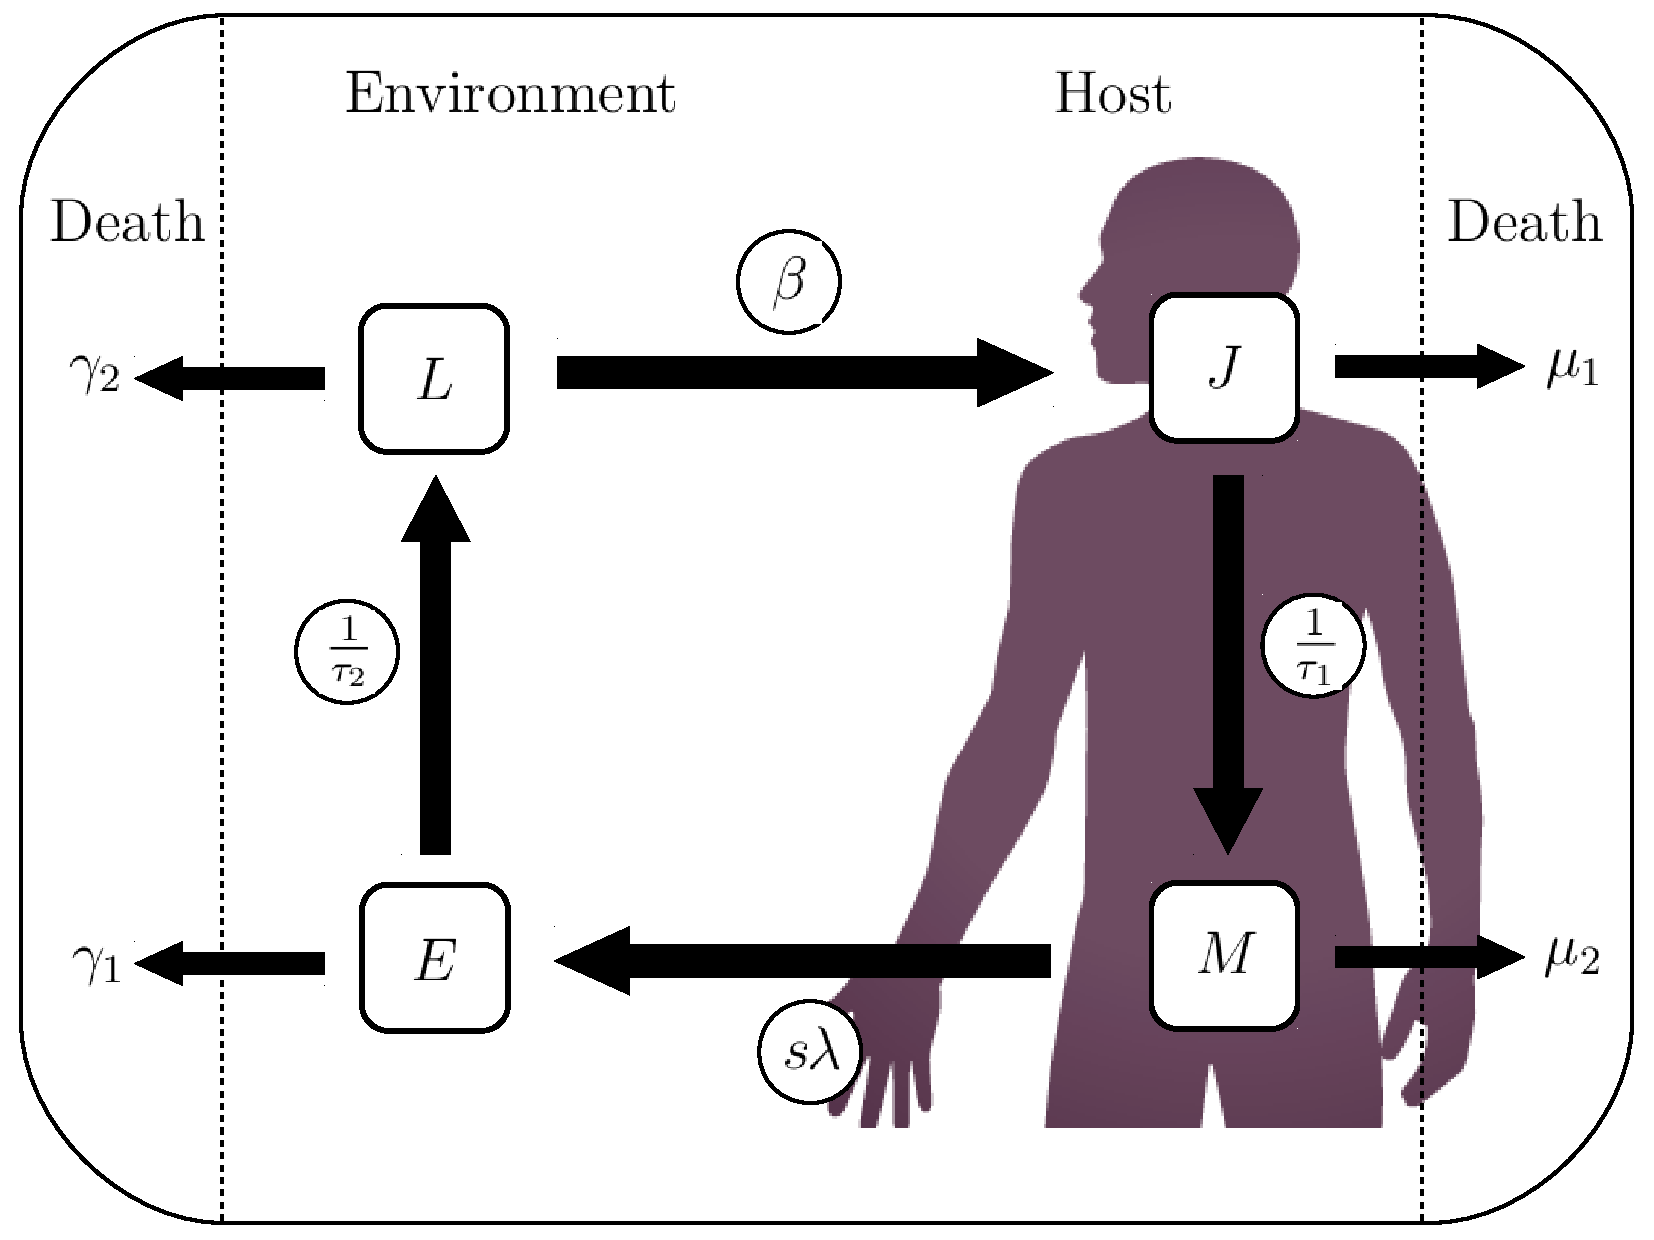
\includegraphics[height=10cm]{Project/Figures/STH/Fig1.pdf}
\caption{{\bf \textit{A. lumbricoides} life cycle.} Diagram depicting the model structure used to represent the \textit{A. lumbricoides} life cycle.}
\label{Fig1}
\end{figure}

Death rates $\mu_1$ and $\mu_2$ for the within-host stages, $J$ and $M$, incorporate both parasite and host mortality. For the environmental stages, $E$ and $L$, death is taken to occur at rates $\gamma_1$ and $\gamma_2$ respectively. The excretion rate of eggs into the environment, $sN\lambda M$, is calculated using the worm gender ratio, $s=0.5$, the worm fecundity, $\lambda$, the human population size, $N$, and the current level of mean worm burden, $M$. Ingestion occurs at rate $\beta L$ per host, removing eggs from the environment at rate $\beta NL$, where $\beta$ represents an ingestion uptake rate. 

All biological processes occurring during environmental stages are considered to be affected by seasonal factors; parameters for egg maturation time ($\tau_2$), egg mortality ($\gamma_1$) and infective stage mortality ($\gamma_2$) are linked to temperature through experimental data, whereas transmission ($\beta$) is taken to vary with rainfall. Values of model parameters are given in Table \ref{table:paramSTH}.

\begin{table}[!ht]
%\begin{adjustwidth}{-2.25in}{0in} % Comment out/remove adjustwidth environment if table fits in text column.
\centering
\caption{
{\bf Model parameter definitions and values.}}
\begin{tabular}{|l|l|l|l|}
\hline
\multicolumn{1}{|l|}{\bf} & \multicolumn{1}{|l|}{\bf Definition} &
\multicolumn{1}{|l|}{\bf Value} &
\multicolumn{1}{|l|}{\bf Source} \\ \hline
$\beta$ & Ingestion or uptake rate & $10^{-12}$--$3.3\times10^{-9}$ & \\ \hline
$\tau_1$ & Maturation rate from juvenile stage to adult worm & 65 (50--80) & \cite{Anderson1992} \\ \hline
$1/\tau_2$ & Mean maturation time from eggs to infective larvae & 15--120 & \cite{Wagner,Arene,Kim} \\ \hline
$d_1$ & Proportion of juvenile stages that survive maturation & 0.01 & \cite{Anderson1992} \\ \hline
$d_2$ & Proportion of eggs that survive to become infective & 0--0.8 & \cite{Arene} \\ \hline
$\mu$ & Death rate of hosts (lifespan = 50 years) & $5.48\times 10^{-5}$  &  \\ \hline
$\mu_1$ & Death rate of juvenile worms (including host death) & $(1-d_1^{1/\tau_1}) + \mu$ &  \\ \hline
$\mu_2$ & Death rate of adult worms (including host death) & 0.042 + $\mu$ & \cite{Anderson1992} \\ \hline
$\gamma_1$ & Death rate of immature eggs & $(\frac{1}{d_2}-1)/\tau_2$ &  \\ \hline
$1/\gamma_2$ & Life span of infective larval stages & 5--65 & \cite{Arene} \\ \hline
$s$ & Sex ratio in adult worms (proportion female) & 0.5 & \cite{Anderson1992} \\ \hline
$\lambda_0$ & Baseline fecundity per adult female worm & $7.03\times 10^5$ & \cite{Churcher} \\ \hline
$N$ & Host population size & setting & \\ \hline
\end{tabular}
\begin{flushleft} Unless specified all units are in days.
\end{flushleft}
\label{table:paramSTH}
%\end{adjustwidth}
\end{table}

% %
%  Want another table later (results?) for fitted relationships??

\subsection{Egg survival data}

To form an evidence-base for relationships between biological model parameters and temperature we have drawn on three different experimental studies considering \textit{A. suum} eggs. Two of these studies have been used to parameterise the average time taken for eggs to mature into infective larvae ($\tau_2$) across temperatures ranging from 5-35\textdegree{C} \cite{Wagner,Kim}. The third study was used for seasonal parameterisation of the immature egg and infective larval death rates ($\gamma_1$ and $\gamma_2$), with a temperature range of 15--35\textdegree{C} \cite{Arene}.

The first study \cite{Wagner} investigated the rate of development to infectivity of a suspension of \textit{A. suum} eggs in flasks placed inside a pig barn in Saskatchewan, western Canada. Recorded temperatures in the barn ranged from 16.8-25.5\textdegree{C} and increased rates of maturation were seen at higher temperatures; it took an between 21-28 days to observe development for temperatures above 23.5\textdegree{C}, whereas a development time of 77-84 days was recorded for a mean barn temperature of 16.8\textdegree{C}. This data was used as the main basis for the relationship between temperature and egg maturation time ($\tau_2$).

The second study \cite{Kim} recorded the developmental stages of eggs in a coarse sand medium in an environmental chamber with 50\% humidity under three temperature conditions: 5\textdegree{C}, 25\textdegree{C} and 30\textdegree{C}. As the humidity was maintained it can be assumed that this was not a limiting factor in development, giving temperature as the sole determinant. No development was observed at 5\textdegree{C} in the first month, with only marginal development being recorded across the three-month time-span of the study; no eggs reached infectivity. At 25\textdegree{C} and 35\textdegree{C} it took 19 and 17 days respectively for eggs to display successful embryonation. This data was used to extend the previous data set to consider a wider range of temperatures in fitting $\tau_2$.

For the two external stage death rates a third study was used \cite{Arene} that considered larval viability post-development and larval death rate across a temperature range of 16-34$\,^{\circ}{\rm C}\pm1$. Eggs were incubated in flasks containing a H$_2$SO$_4$ solution so moisture is also assumed to be sufficient for development and survival. Higher temperatures recorded lower viability and faster time to 90\% mortality; larvae were observed as living for up to 150 days at temperatures of around 20\textdegree{C}, but above 25\textdegree{C} this quickly drops to below 50 days and above 30\textdegree{C} larvae survived for fewer than 10 days. The study also considered development rate, but recorded the time until 90\% of the eggs had reached maturity rather than the average; this was used to provide a qualitative validation of the fitted relationship for $\tau_2$ but not considered for fitting purposes.

All seasonal egg relationships were fitted using fminsearch in Matlab R2015b to minimise the squared error between the model and the data. An exponential decay curve was fitted to the maturation time data as a function of temperature; limits of function parameters give $\tau_2$ bounded below by a non-zero limit and the exponential relationship reflects the assumption that development occurs either very slowly or not at all for low temperatures \cite{Kim}. The proportion of eggs successfully reaching maturity ($d_2$) was fitted to a quartic relationship for higher temperatures and capped at a fitted maximum for lower temperatures. Immature egg death rates ($\gamma_1$) were then calculated as values which would give the associated survival proportions; $\gamma_1 = (\frac{1}{d_2}-1)/\tau_2$. Larval death rates ($\gamma_2$) were derived by solving a simple differential relationship to get $\gamma_2 = -\ln{(0.1)}/m$ where $m$ is the time taken to achieve 90\% mortality, which was fitted to an inverse tangent relationship with temperature. 

Full temperature-dependent relationships are detailed in the Results in Table \ref{tab:seas}.

\subsection{Climate data}

Records of mean monthly temperature (\textdegree{C}) and rainfall (mm) relevant to the dates and settings we chose to investigate are taken from web archives \cite{Ktemp,Ntemp} and used to fit setting-specific functions. The main requirement of these functions is annual periodicity, hence a sinusoidal function provides a good approximation. 

\subsection{Epidemiological data}

The first data set used to fit and validate the model originates from a field study conducted between April 1977 and September 1978 in Gyeonggi Province, South Korea \cite{Seo}. The study was conducted across six hamlets (labeled A-F), each consisting of approximately 100 inhabitants, that were considered far enough apart to have independent transmission. Three rounds of biannual testing and chemotherapy were applied in each location to the entire village population, with intervention dates offset by a month for each hamlet to monitor different seasonal responses. The drug used was pyrantel pamoate and the test was a Kato-Katz smear test, involving visual characterisation of absence or presence of eggs in a stool sample.

The second data set, used to investigate an alternative setting, is taken from a double-blind placebo-controlled random trial study based across four semi-urban villages in Osun State, Nigeria, between 2006 and 2007 \cite{Kirwan}. Participation was encouraged but voluntary and the study followed 194 children, aged 12-60 months, across a period of 14 months. The treatment group received directly observed therapy (DOT) of albendazole every 4 months for a year, with a follow-up assessment at 14 months; the control group received no treatment but prevalence was measured at the same intervals as the treatment group. The test used in both cohorts was also a Kato-Katz smear test.

\subsection{Model implementation and fitting}

The model was coded and run using Matlab R2015b, with the function ode45 used to compute numerical solutions to the differential equations. For each simulation the model was run for a 30 year period to equilibriate the initial conditions before any intervention strategy was applied. Administration of anthelmintic drugs was implemented as a proportional reduction in mean worm burden; this proportion depended on efficacy, taken from the literature, and coverage, taken from the data. Treatment using albendazole was assumed to have an efficacy of $88$\% \cite{Keiser}; pyrantel pamoate is taken to have the same efficacy \cite{Keiser}, although this is likely to be a conservative estimate \cite{Albonico}.

In both settings transmission rate ($\beta$) was originally considered as an inverse tangent function of rainfall; three parameters are taken to describe the magnitude ($\beta_0$), slope gradient ($a_1$), and horizontal shift ($a_2$) of the function. The slope gradient and shift are permitted to take a range of values to allow for either a positive or negative relationship to reflect conflicting views in the literature and as it is possible that this will change between settings due to influence from human behavioural characteristics, such as the effects of rice planting during the rainy season. 

\begin{figure}[!h]
\begin{center}
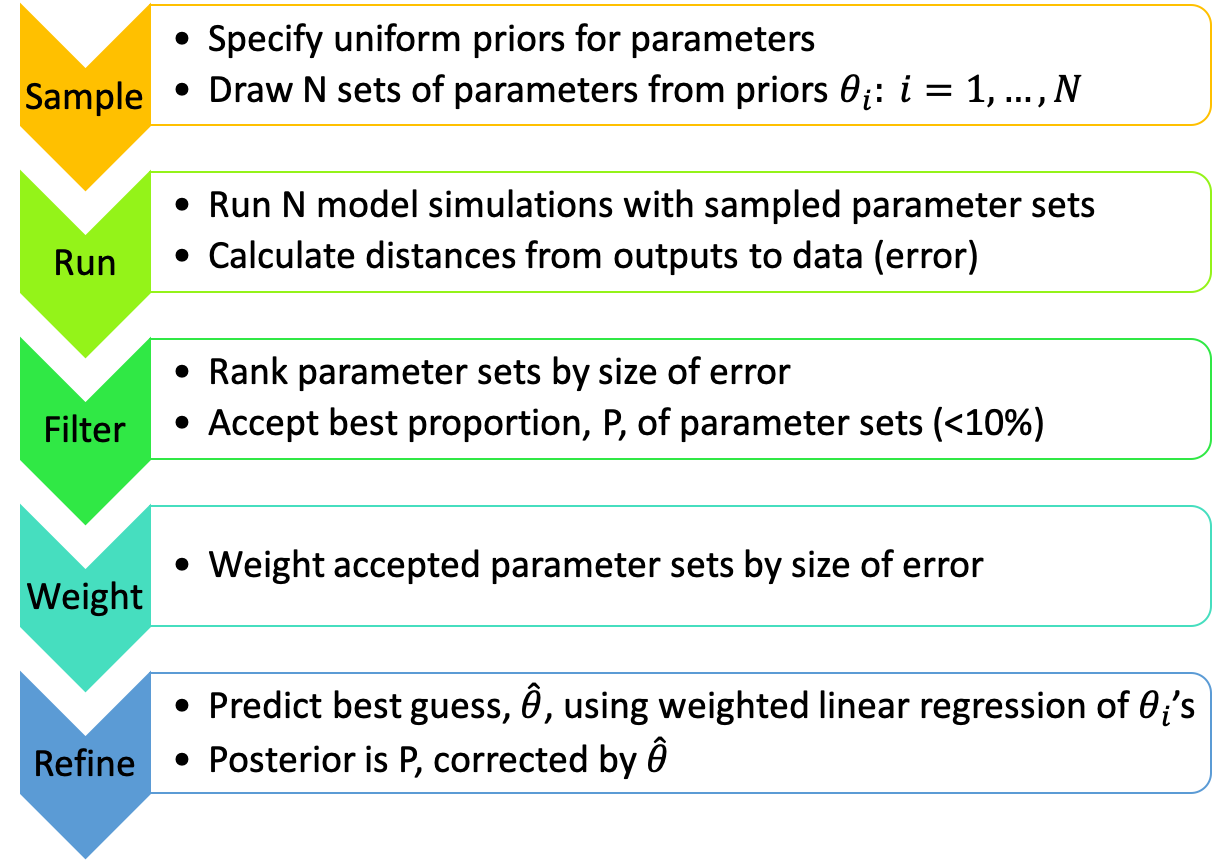
\includegraphics[height=10cm]{Project/Figures/STH/ABCdiag.png}
%\begin{adjustwidth}{-2.25in}{0in}$ % Comment out/remove adjustwidth environment if table fits in text column.
\caption{{\bf ABC-CDE.}
Schematic demonstrating the approximate Bayesian computation regression-based conditional density estimate method used to fit parameters.}
\label{fig:ABCdiag}
%\end{adjustwidth}
\end{center}
\end{figure} 

Parameters were fitted to the epidemiological data sets using approximate Bayesian computation (ABC), followed by a regression-based conditional density estimation method (ABC-CDE) \cite{Beaumont}, see Figure \ref{fig:ABCdiag}. Uniform priors for each of the fitted parameters were defined and simulations were run using values sampled from these distributions. Simulation outputs were compared to prevalence data, filtered, and then linear regression is used to correct model inputs, resulting in a posterior distribution. Simulation outputs were filtered (keeping 1000 of 75K realisations, or 1.3\%) to maximise the binomial log-likelihood: 

\begin{equation}
\sum_{i}[x_i\log(p_i)+(N-x_i)\log(1-p_i)]\,, 
\end{equation}

where $x_i$ were the positive cases from the data, $N$ was the total population size and $p_i$ were the model prevalences. Weights were then calculated using the squared errors between the model output and the data and the posteriors were corrected by the best estimate of the underlying parameters, calculated using weighted linear regression of all filtered parameter sets.

Model outcomes were obtained from 1000 model runs sampling parameters from the posterior distributions and credible intervals were calculated by taking the 2.5\% and 97.5\% quantiles of the outputs.

For the South Korean data set the 9 data points from villages A-C were used together for fitting and then model outputs for villages D-F were compared to the other half of the data for validation. Prevalence, $P$, in the host population was calculated from mean worm burden using a standard negative binomial relationship \cite{Anderson1992}, $P = 1-(1+M/k)^{-k}$, to capture the expected heterogeneity of infection intensity.

For the Nigerian data set the model was fitted to the first four data points for each group and then the model predictions were compared to the fifth data point in each case. Due to results displaying a very low overall impact of rainfall on transmission the model was also fitted assuming a constant transmission rate, $\beta$, and Akaike Information Criterion (AIC) and AICc (AIC with a correction for small sample sizes) values were used for model selection. A negative binomial relationship was also assumed between prevalence and mean worm burden, but in this case the aggregation parameter was also fitted to the data.

% Results and Discussion can be combined.
\section{Results and Discussion}

\subsection{Egg survival parameters}

The experimental data for all three environmental egg parameters showed strong dependence on temperature, as seen in Figure \ref{Fig2}. The biggest effects are seen in maturation for temperatures below 20\textdegree{C}, for infective stage mortality above 25\textdegree{C}. The proportion of eggs that develop into viable larvae is mostly constant unless temperatures reach above 30\textdegree{C}, which is only relevant in some climates.  All fitted seasonal relationships can be seen in Table \ref{tab:seas}.

Standard transmission models for human ascariasis would expect maturation time to be in the range of 10 to 30 days and a free living infective stage life expectancy of 28 to 84 days \cite{Anderson1992}. The fitted relationships fall in the 10-30 day range for temperatures above approximately 22.5\textdegree{C}, but exhibit a dramatic increase for lower temperatures. For mid-range temperatures the model predicts time to 90\% mortality for infective stages to be between 40 and 120 days, which equates to a life expectancy of 17-52 days and falls within the expected range.

\begin{sidewaysfigure}[p] % Comment out/remove adjustwidth environment if table fits in text column.
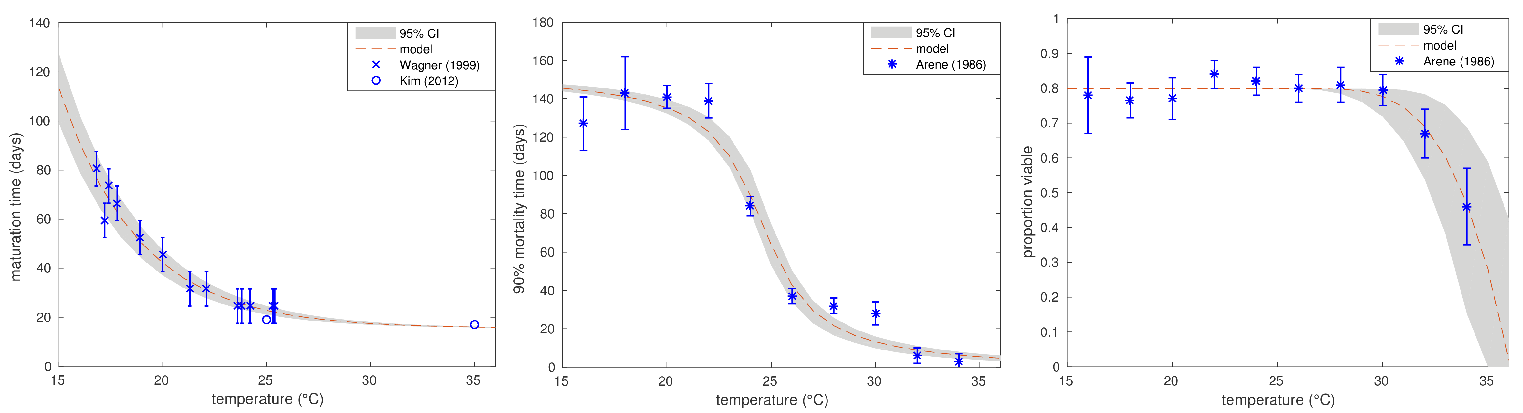
\includegraphics[height=6cm]{Project/Figures/STH/Fig2.pdf}
\caption{{\bf Environmental egg relationships.}
Fitted relationships for environmental egg parameters with temperature compared to the data. Left: Maturation time (days). Middle: Time to 90\% mortality (days). Right: Proportion of eggs that develop into viable larvae.}
\label{Fig2}
\end{sidewaysfigure} 

\FloatBarrier

\begin{sidewaystable}[p]
\centering
\caption{
{\bf Fitted equations and parameters for seasonal relationships with temperature (\textdegree{C}), $T$.}}
\begin{tabular}{|l|l|l|l|l|l|}
\hline
\multicolumn{1}{|l|}{\bf Name} & \multicolumn{1}{|l|}{\bf Process} &
\multicolumn{1}{|l|}{\bf Relationship} & \multicolumn{1}{|l|}{\bf $a_1$} &
\multicolumn{1}{|l|}{\bf $a_2$} & \multicolumn{1}{|l|}{\bf $a_3$}  \\ \hline
$\tau_2$ & Maturation ($E$) & $a_1 + a_2\exp(-a_3T)$ & $15.5 (13.0,17.3)$ & $4.49(3.33,5.35)\cdot10^3$ & $0.255(0.231,0.267)$\\ \hline
$m$ & 90\% mortality ($L$) & $a_1(\arctan(a_2-a_3T)+1.5)$ & $50.2(48.4,52.3)$ & $13.7(11.2,16.2)$ & $0.558(0.457,0.660)$\\ \hline
$d_2$ & Proportion viable & $\min(a_1, a_1-a_2(T-a_3)^4)$ & $0.798(0.796,0.801)$ & $1.08(0.62,1.78)\cdot10^{-5}$ & $26.3(25.4,26.9)$  \\ \hline
\label{tab:seas}
\end{tabular}
\begin{flushleft}
\end{flushleft}
\end{sidewaystable}

% Place figure captions after the first paragraph in which they are cited.
\subsection{Fitting and validation: Korea}

The fitted parameters for transmission rate in South Korea are: $\beta_0 = 3.30 (2.89,3.82)\times10^{-9}$; $a_1 = -3.46(-3.97,-3.12)$; $a_2 = -66.8(-85.3,56.0)$; such that the transmission rate $\beta= \frac{a_1}{\pi}(\arctan(a_2R+a_3)+\pi/2)$.  This reflects an inverse relationship between rainfall and transmission, perhaps due to high rainfall resulting in infective stages being washed away from areas where uptake is likely to occur.

Figure \ref{Fig7} shows the fitted rainfall-dependent relationship for South Korea. Transmission is at its lowest during the months that see the most rain, with a sharp increase as rainfall declines into the driest months. This could be due to heavy rain washing eggs away through drainage systems, hence reducing transmission, or human behavioural traits.

\begin{figure}[!h]
\begin{center}
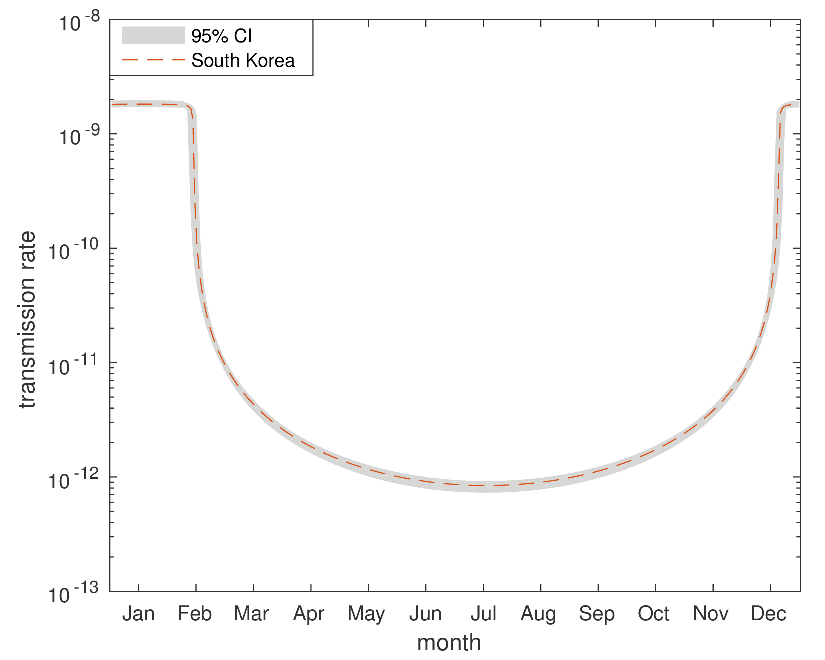
\includegraphics[height=8cm]{Project/Figures/STH/Fig7.pdf}
%\begin{adjustwidth}{-2.25in}{0in}$ % Comment out/remove adjustwidth environment if table fits in text column.
\caption{{\bf Seasonal transmission.}
Annual values for the transmission rate ($\beta$) in Osun, South Korea. Depicted as best fit model averages with 95\% credible intervals.}
\label{Fig7}
%\end{adjustwidth}
\end{center}
\end{figure} 

Figure \ref{Fig3} shows both the fitting and validating outcomes for the South Korean data set. There is excellent agreement between the model and the data used for fitting from villages A-C. Model outcomes for villages D and E are seen to provide a reasonable fit to the data when considering overlap between the respective 95\% confidence intervals, with some discrepancy between the model and the data for village F. Parasite density aggregation, $k$, is $0.45$ \cite{Chai,Guyatt}.

% Place figure captions after the first paragraph in which they are cited.
\begin{figure}[!h]
% Comment out/remove adjustwidth environment if table fits in text column.
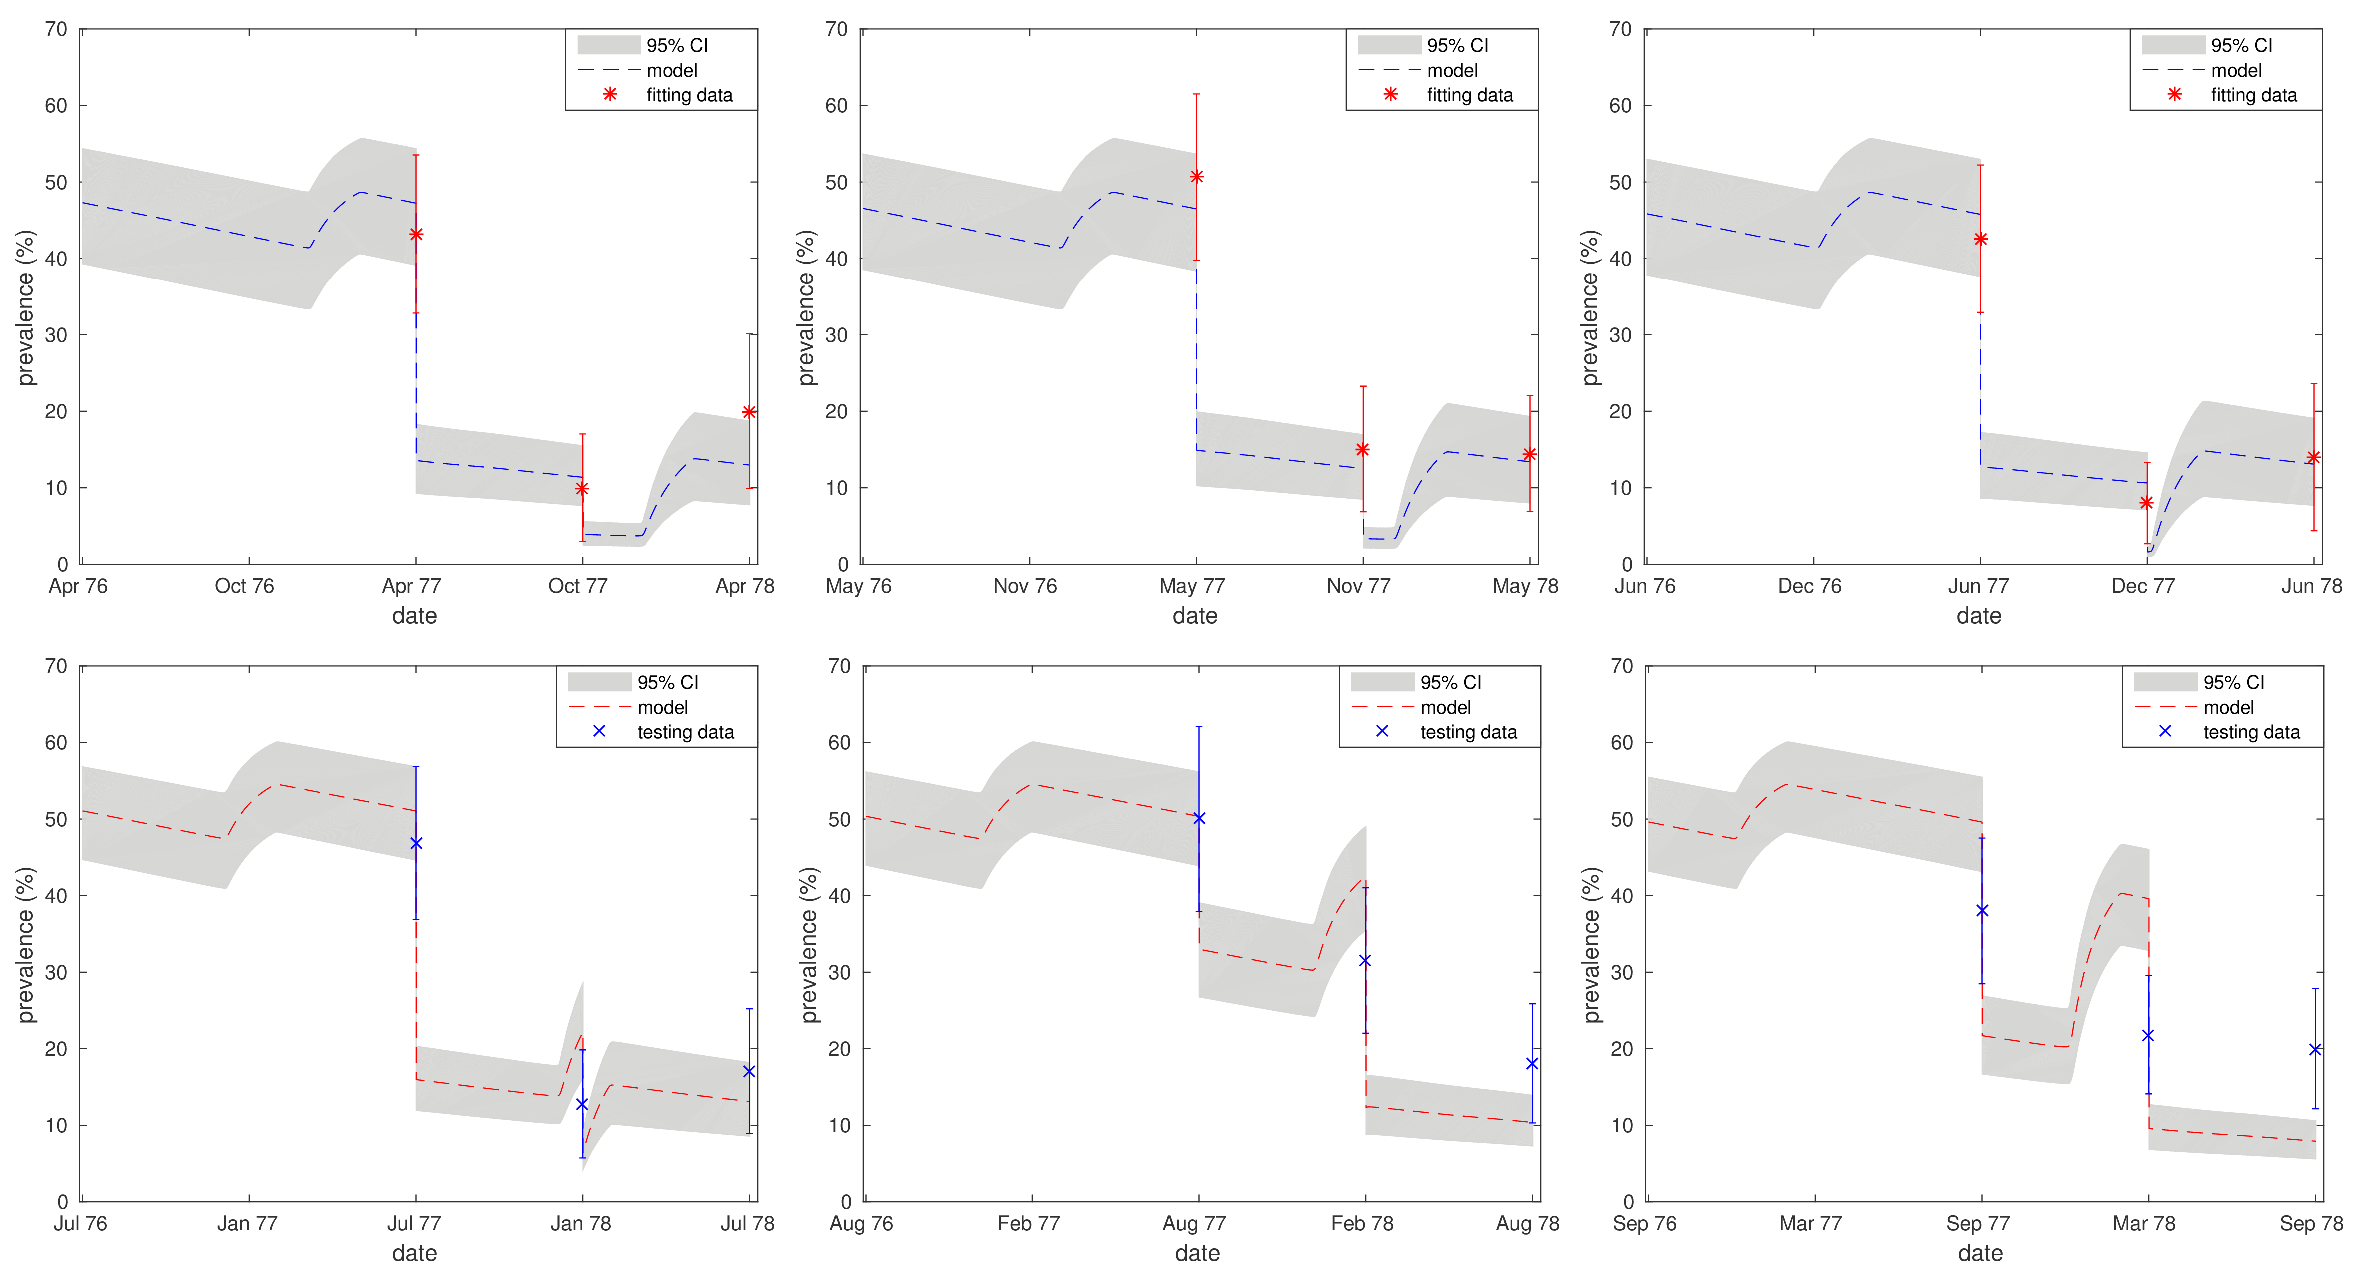
\includegraphics[height=7.5cm]{Project/Figures/STH/Fig3.pdf}
\caption{{\bf Model validation -- South Korea.}
Fitting and testing plots for Villages A-F \cite{Seo}. 95\% confidence is represented by error bars on the data and 95\% credible intervals by shaded regions on the model outcome. Top row (left to right): Villages A-C, fitting outcomes (- -) compared with data ($*$). Bottom row (left to right): Villages D-F, model outcomes (- -) compared with data ($\times$). Prevalence data was recorded pre-treatment in all cases.}
\label{Fig3}
\end{figure} 

\subsection{Fitting and validation: Nigeria}

% Results: Re-phrase “rejection” of the model for Nigeria, make it clear that rainfall is rejected but not temperature 

ABC results for fitting the model to the Nigerian data returned posteriors that allowed for a range of marginal positive and negative relationships between rainfall and transmission, indicating a lack of evidence to support this element of model structure, unlike the significant relationship found for the South Korean data. Comparing the sample size corrected Akaike Information Criterion (AICc) of this model $AICc_{R}$ to that of the reduced model ($AICc_{\beta}$), considering constant transmission, leads us to reject the combined model with rainfall in favour of one relying on temperature ($AICc_{R}=434.83$; $AICc_{\beta}=429.69$; $AICc_{\beta}<AICc_{R}$; the relative likelihood of the rainfall model is 0.082). Comparison of the less conservative AIC values would also reject the rainfall model in favour of the simpler one ($AIC_{R}=434.62$, $AIC_{\beta}=429.63$). This implies that we do not have enough evidence to suggest rainfall is a significant predictor of disease in Nigeria. A transmission rate of $\beta=7.93\times10^{-10}$ $(7.86--8.00\times10^{-10}$) and a parasite density aggregation of $k=0.16$ give the best fit to the data.

Fitting outcomes for the constant transmission model capture the overall magnitude and trend of the data in both cases (see Figure \ref{Fig4}), with reasonable agreement between the model and testing data points (August 2007). The model appears unable to capture the observed peak in cases seen across both groups during February 2007, which suggests that this increase was driven by additional factors; it is possible that sampling biases caused by behavioural change among the target population could influence such a peak.

% Place figure captions after the first paragraph in which they are cited.
\begin{figure}[!h]
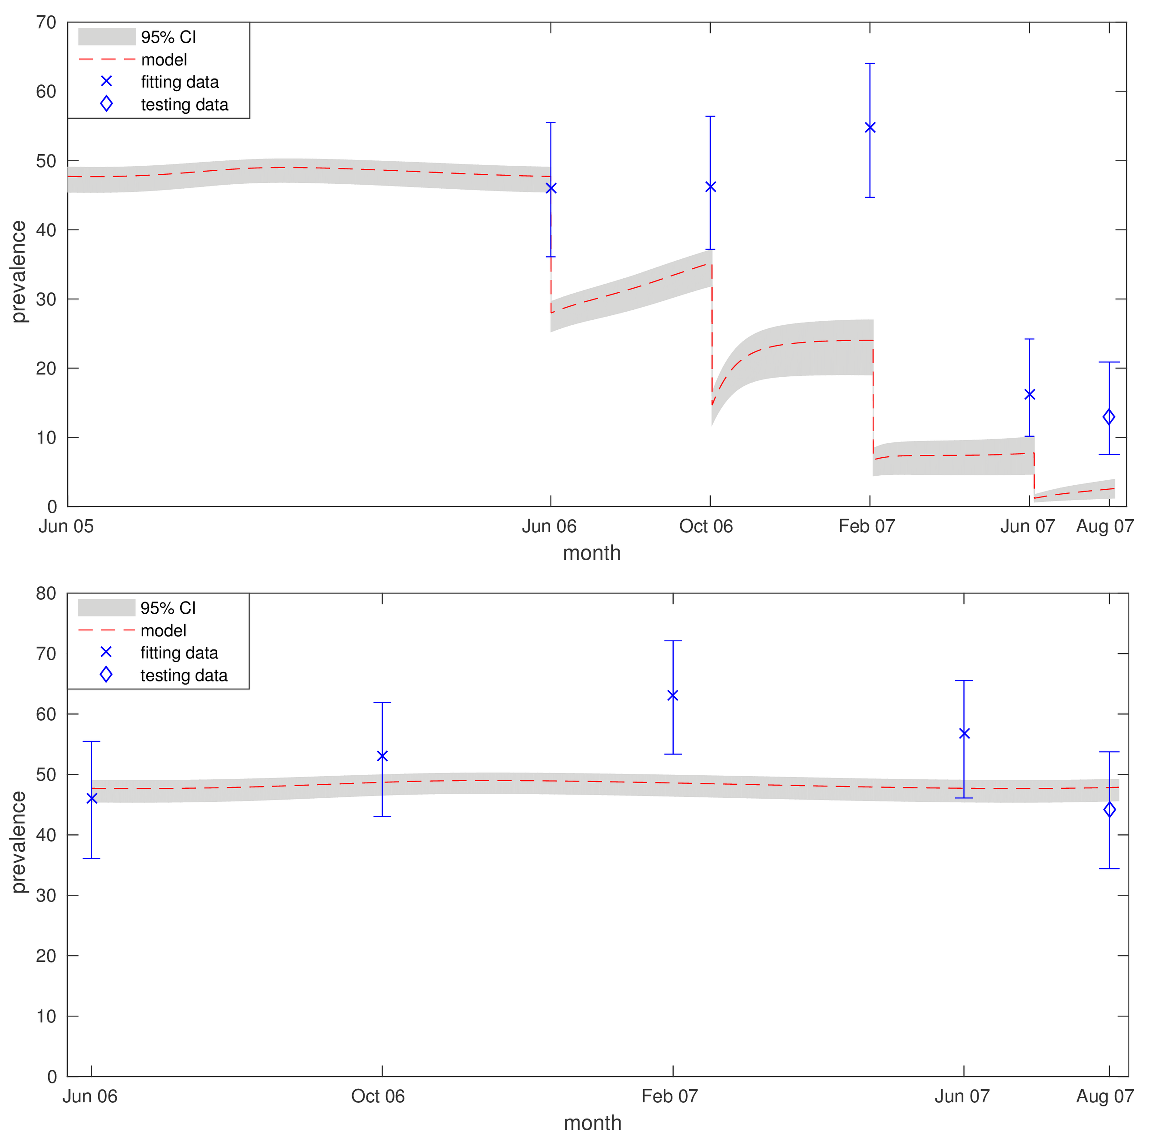
\includegraphics[height=12cm]{Project/Figures/STH/Fig4.pdf}
%\begin{adjustwidth}{-2.25in}{0in}$ % Comment out/remove adjustwidth environment if table fits in text column.
\caption{{\bf Model validation -- Nigeria.}
Fitting plots for treatment (top) and control (bottom) branches of the 2006-07 Nigerian study \cite{Kirwan}. 95\% confidence, for the data, and 95\% credible intervals, for the model, are represented with error bars and shaded regions respectively. The model (- -) was fitted to the first four data points in each branch ($\times$) and then compared to the fifth observation ($\diamond$).}
\label{Fig4}
%\end{adjustwidth}
\end{figure} 

\subsection[Egg dynamics]{Seasonal egg dynamics}

Figure \ref{Fig6} shows the model estimates for setting-specific seasonal parameter values. The maturation time relationships show a key difference between the two settings; in Nigeria the high temperatures result in low-level fluctuations in maturation time around the 20 day mark, but the drop-off in temperature over the winter in South Korea is expected to produce a significant slow down in maturation across this period - with more than half the year seeing average maturation times of greater than 50 days.

\begin{figure}[!h]
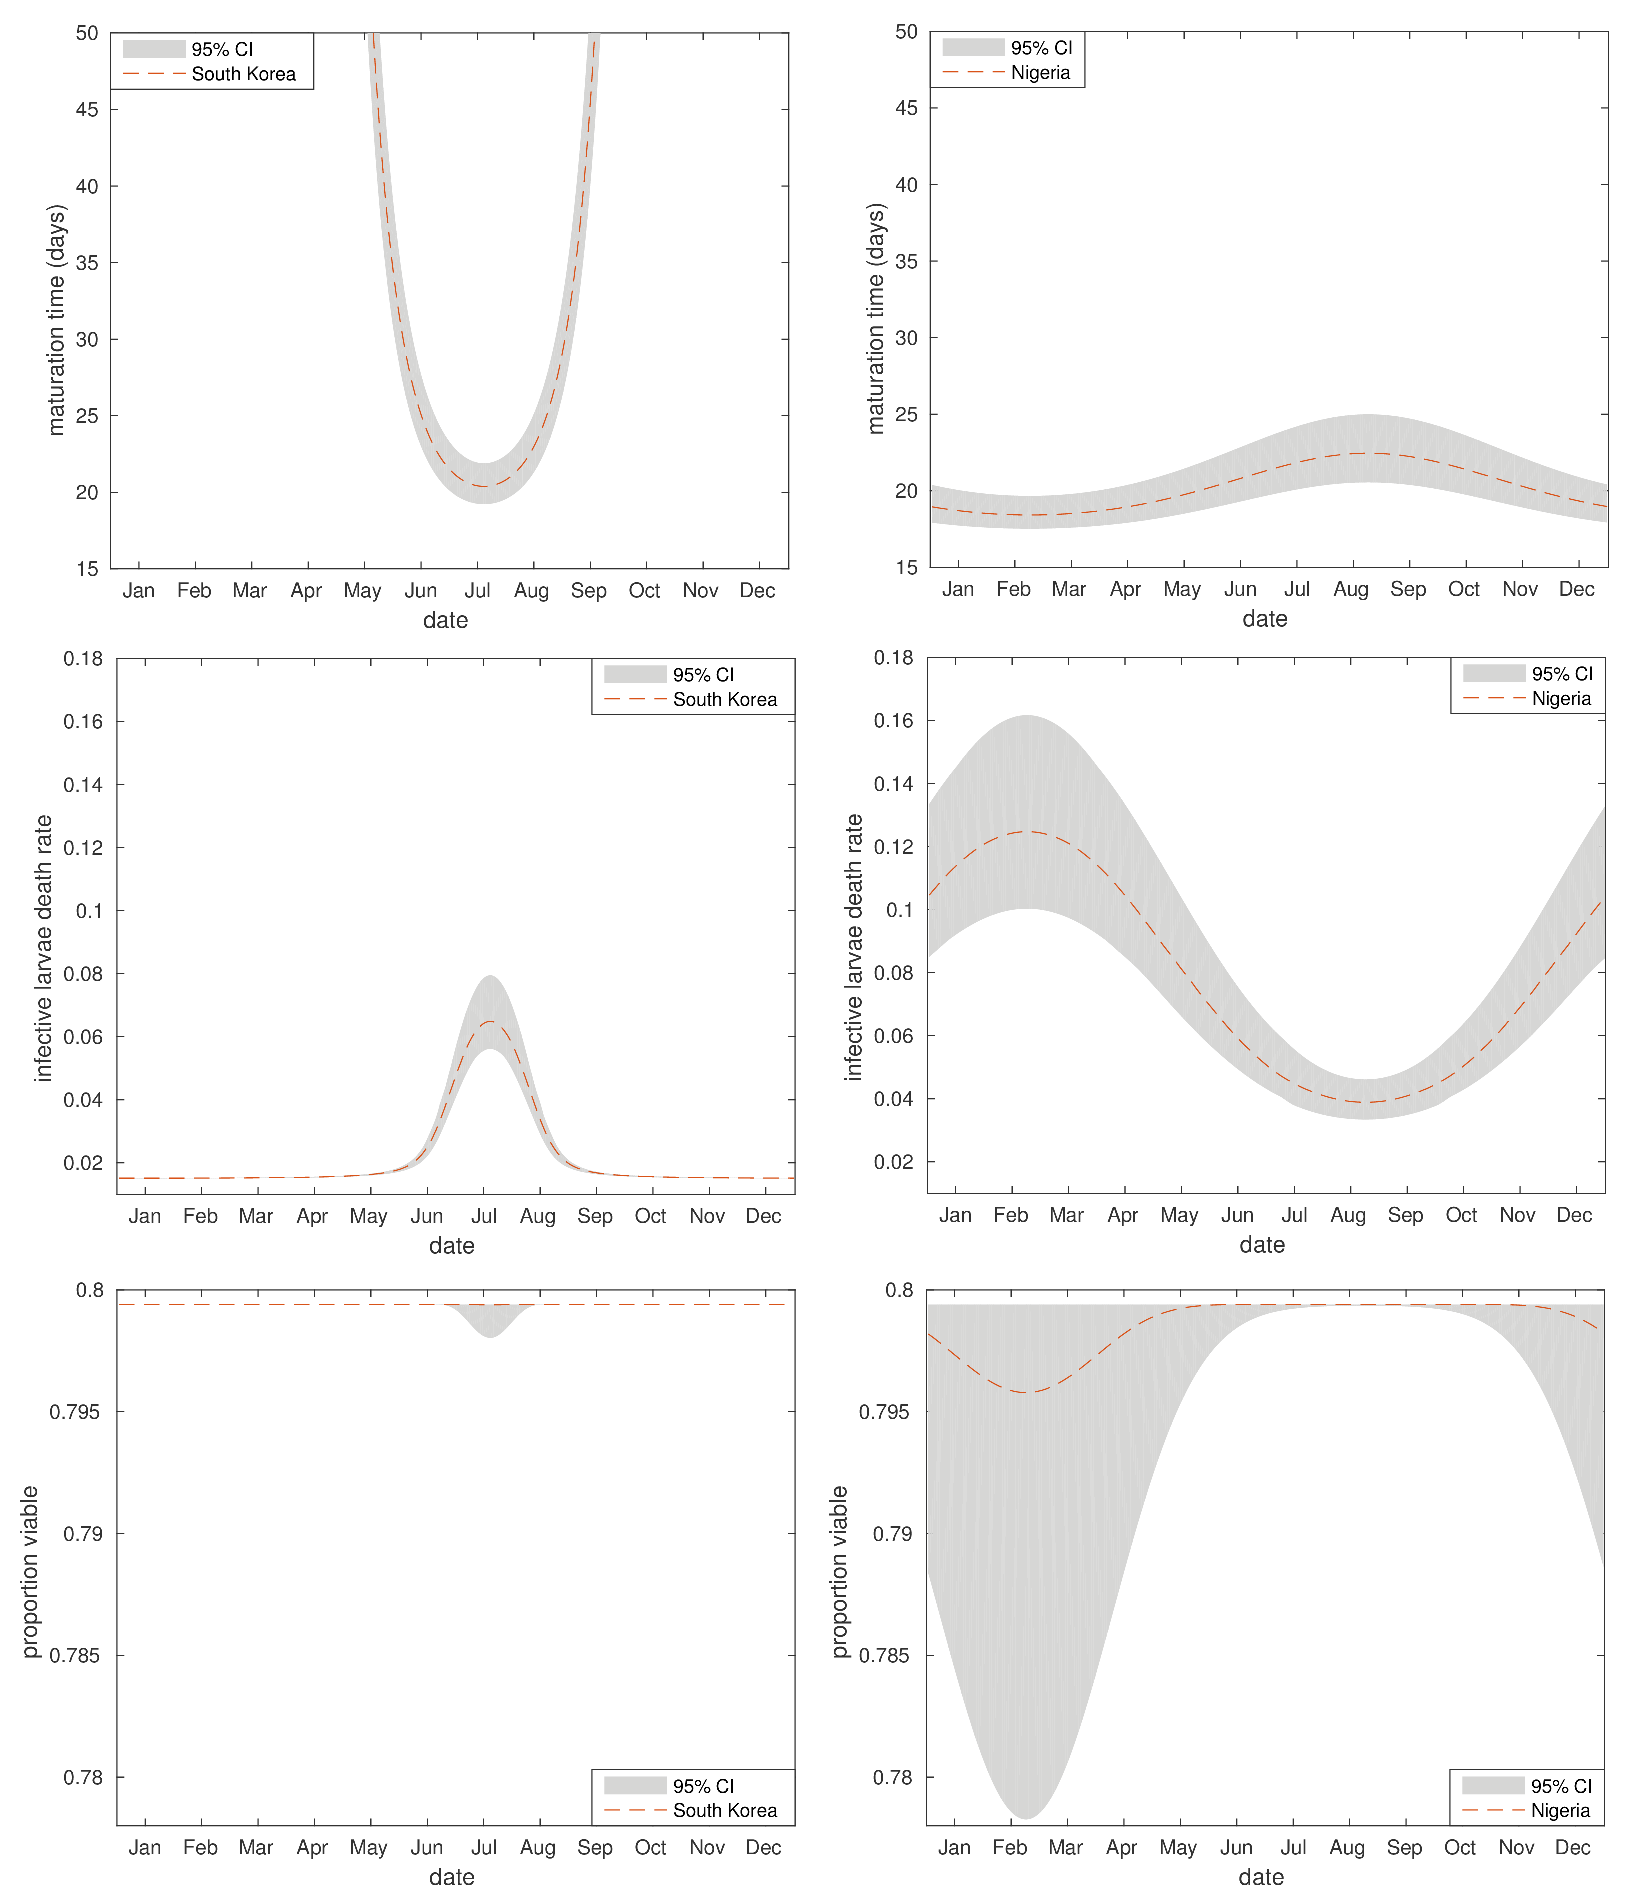
\includegraphics[height=16cm]{Project/Figures/STH/Fig6.pdf}
%\begin{adjustwidth}{-2.25in}{0in}$ % Comment out/remove adjustwidth environment if table fits in text column.
\caption{{\bf Seasonal external stage parameters.}
Annual parameter values for South Korea (left) and Nigeria (right). From top to bottom: maturation time (days); daily death rate of infective larval stages; proportion of eggs that are viable following maturation. Depicted as best fit model averages with 95\% credible intervals.}
\label{Fig6}
%\end{adjustwidth}
\end{figure} 

In South Korea the model considers larval mortality to be very low across the entire year, due to low overall temperatures, with a peak during the summer months between May and September. In contrast, larval mortality in Nigeria is taken to fluctuate across the year, but with a higher average death rate. However, in both settings the temperatures don't get high enough for the model to predict much effect on the proportion of eggs that remain viable following maturation.


\subsection{Impact on MDA}

Investigating model outcomes for the South Korean setting shows that seasonal timing of MDA could result in a 74.5\% difference in the number of days the average individual is infected with worms (mean worm days) across the 12 months following cessation of MDA; the best and worst case scenarios are March and June respectively. This represents a significant improvement in worm burden across the population, which could be expected to link with similar decreases in morbidity and infection intensity. Similar improvements for prevalence and levels of infectious larvae in environment are detailed in Table \ref{tab:outcome}. It is also interesting to note that whilst the seasonal trend is much more noticeable in the external larval population than the mean worm burden, there is still potential for a large seasonal impact on intervention (see Figure \ref{Fig5}).

\begin{sidewaystable}[p]
\centering
\caption{
{\bf The predicted best and worst treatment months for Gyeonggi Province, South Korea, 1977.}}
\begin{tabular}{|l|l|l|l|}
\hline
\multicolumn{1}{|l|}{\bf Outcome} & \multicolumn{1}{|l|}{\bf June (worst)} &
\multicolumn{1}{|l|}{\bf March (best)} &
\multicolumn{1}{|l|}{\bf Relative improvement} \\ \hline
Mean worm days & 151.6 (112.1 - 202.1) & 38.6 (22.1 - 63.6) & 74.5\% (43.3 - 89.1\%) \\ \hline
Prevalence & 25.4\% (20.9 - 30.3\%) & 9.0\% (5.5 - 13.7\%) & 64.6\% (34.4 - 81.8\%)\\ \hline
Infectious egg count & $6.26\times10^8$ (4.48 - 8.51$\times10^8$) & $1.67\times10^8$ (0.92 - 2.84$\times10^8$) & 73.3\% (36.7 - 89.2\%) \\ \hline
\end{tabular}
\label{tab:outcome}
\begin{flushleft} For the 12 months following cessation of 4 annual treatment rounds; mean worm days represents the total burden of infection per individual whilst other values are averaged across the time period.
\end{flushleft}
\end{sidewaystable}

% Place figure captions after the first paragraph in which they are cited.
\begin{figure}[!h]
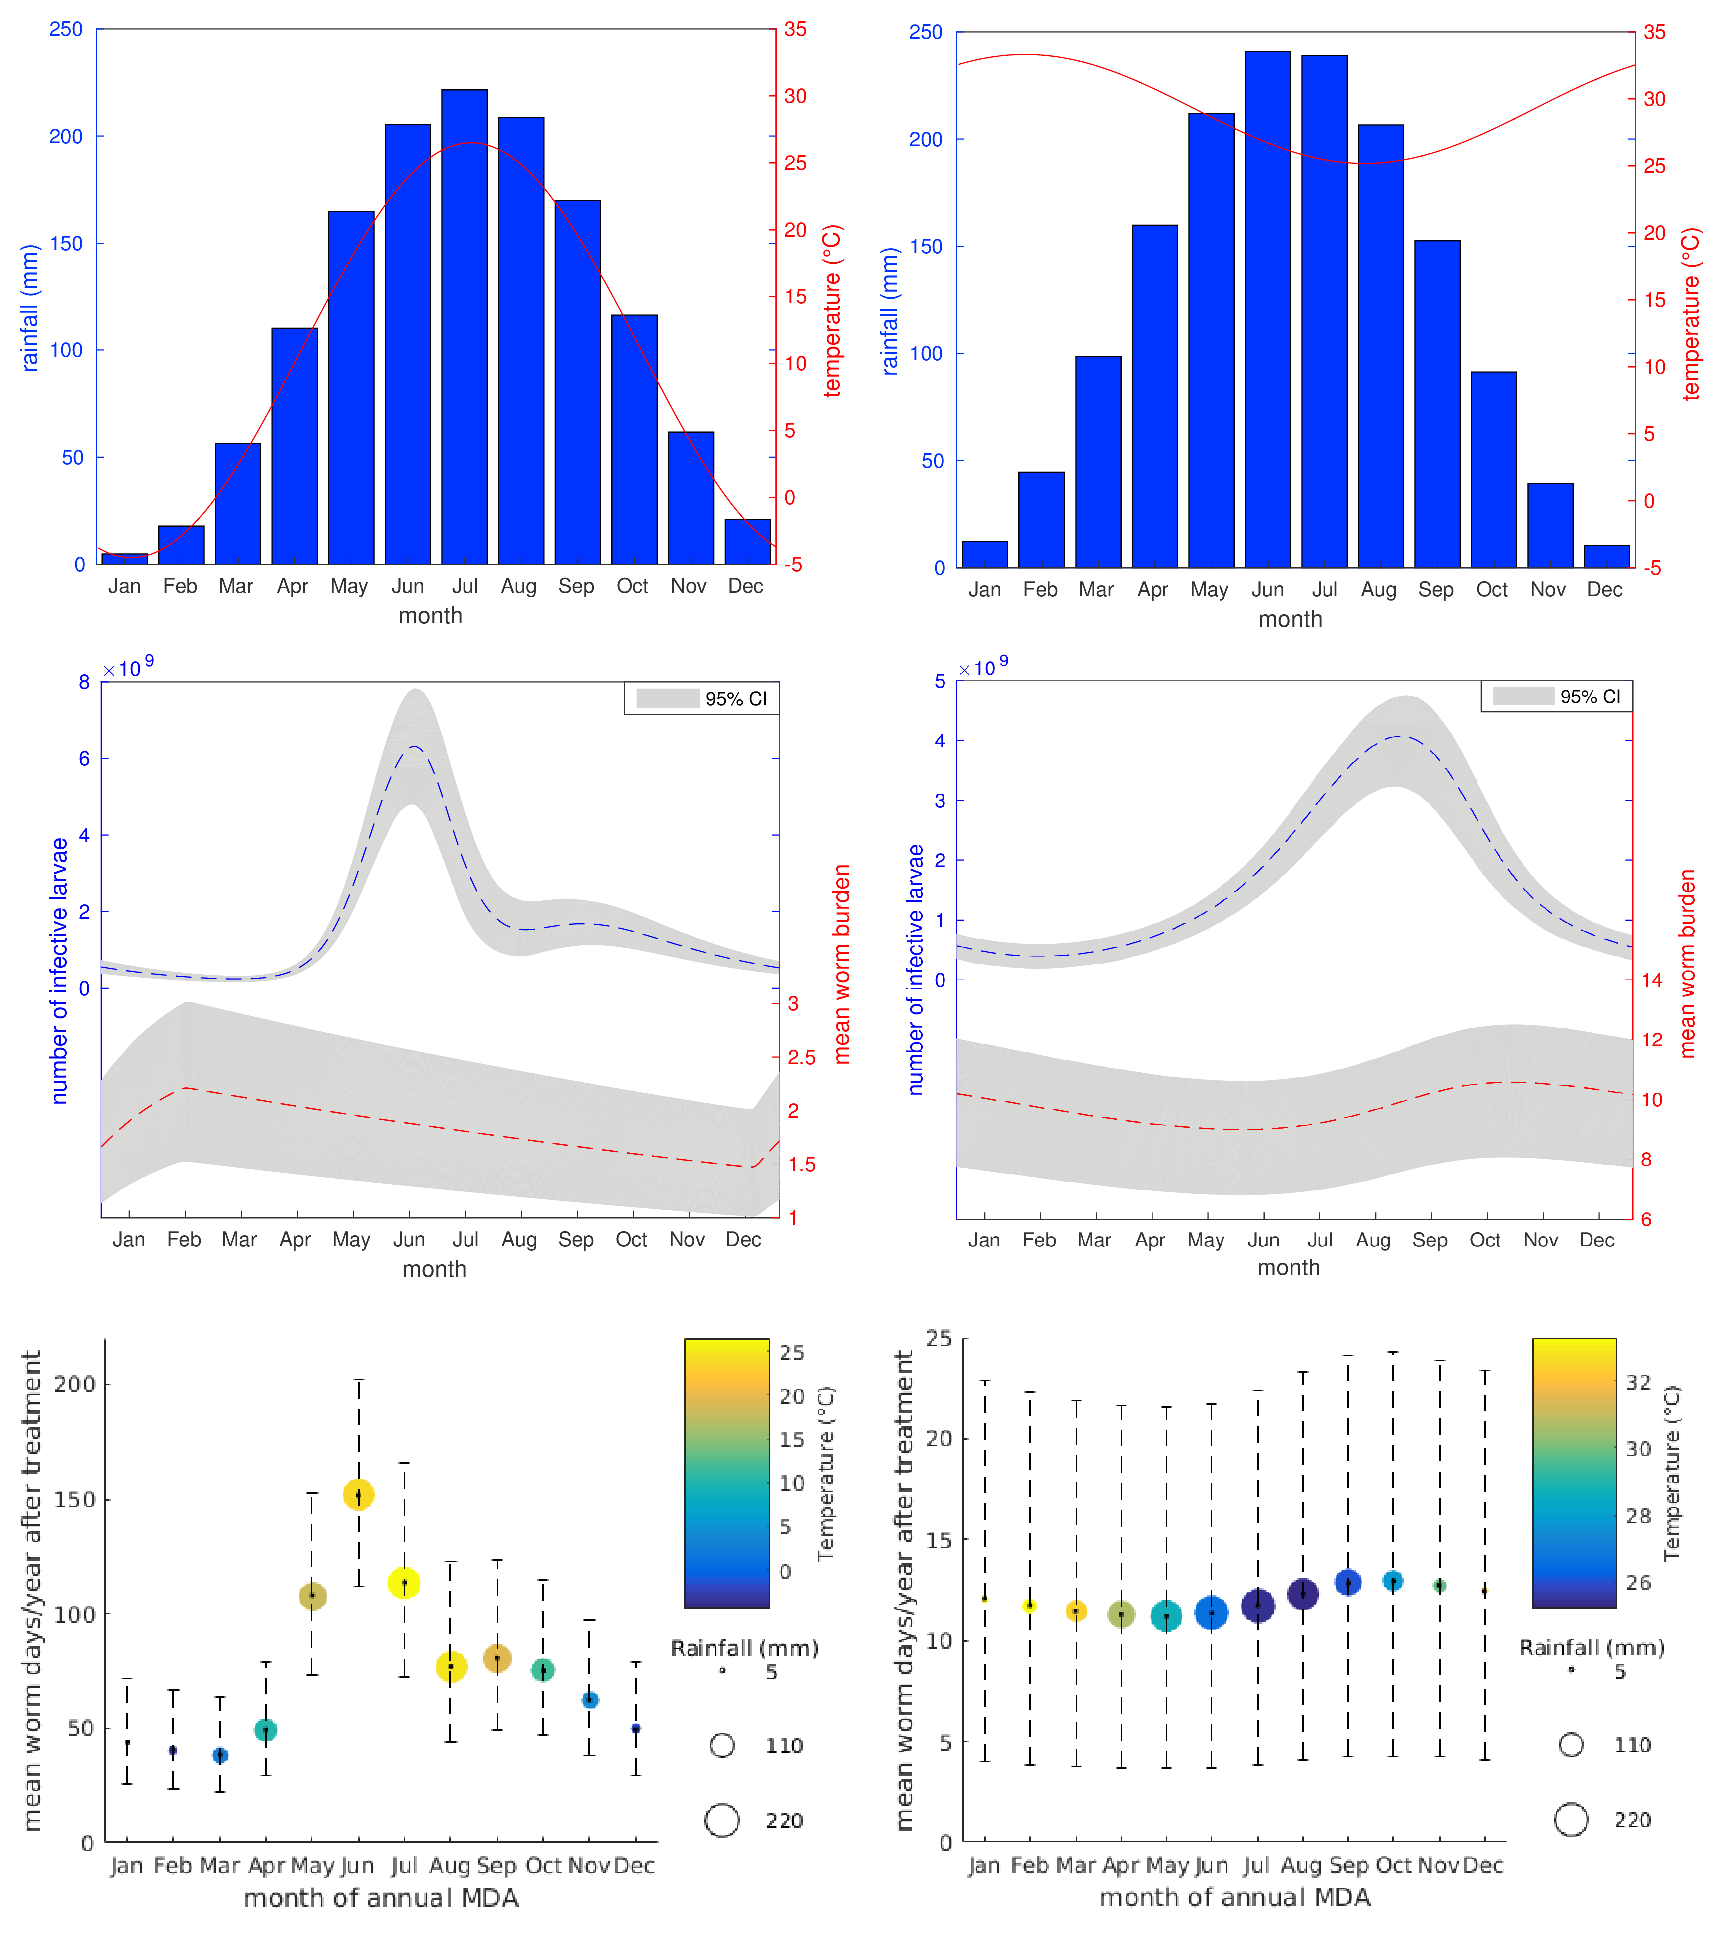
\includegraphics[height=16cm]{Project/Figures/STH/Fig5.pdf}
%\begin{adjustwidth}{-2.25in}{0in}$ % Comment out/remove adjustwidth environment if table fits in text column.
\caption{{\bf Model outcomes.}
Results for South Korea (left) and Nigeria (right). Top row: Fitted temperature and rainfall profiles. Middle row: Seasonal pre-control baseline profiles showing environmental levels of infective larvae and mean worm burden. Bottom row: Predicted mean number of worm days per individual across the 12 months following cessation of 4 annual MDA rounds, for treatment occurring in different months of the year. All error bands represent 95\% credible intervals.}
\label{Fig5}
%\end{adjustwidth}
\end{figure} 

In South Korea June represents a peak in levels of infectious larvae and the beginning of an uptake in transmission across the following months (see Supporting Information for estimated seasonal transmission levels), causing faster reinfection. Bringing down prevalence through MDA also results in low egg output until new adult worm infections have developed (approximately 2-3 months). As larval numbers will be naturally declining in this period it is expected that artificially reducing egg output through mass treatment will have a less marked effect on the overall population.

Contrastingly, in March, infectious larval counts are close to an annual minimum and transmission is on the decline. As the temperature picks up through April and May the larval population should experience a sharp increase, hence treating at this time is likely to limit the resulting peak and dampen future reinfection potential. 

In Nigeria there is still a seasonal peak in environmental levels of infective larvae, but the model does not indicate much difference between MDA outcomes for treatment at differing times of the year (Figure \ref{Fig5}, bottom right). This comes partially from the lack of rainfall dependence, but also due to the narrow temperature range in the region; for temperatures above 25$^{\circ}$C both the egg maturation and larval death rates show very little variation, resulting in a reduced seasonal effect -- see Supporting Information for estimated parameter values across the year.

In both cases the best time for annual treatment is predicted to occur just before the main upswing in infective larvae, the worst time coinciding with the peak. Bringing down infection levels whilst larval numbers are low starves the larval population, causing larger reductions in future infection levels; decreased transmission due to high rainfall in the summer months in South Korea exaggerates this effect.

Figure \ref{Fig8} shows the average predicted prevalence in the 12 months immediately following 4 rounds of seasonally-timed annual MDA, with treatment times during different months of the year, for both settings. We see a very similar trend to the mean worm days plots in Figure \ref{Fig5}, with large seasonal differences in South Korea and no evidence for any significant difference in Nigeria.

\begin{figure}[h]
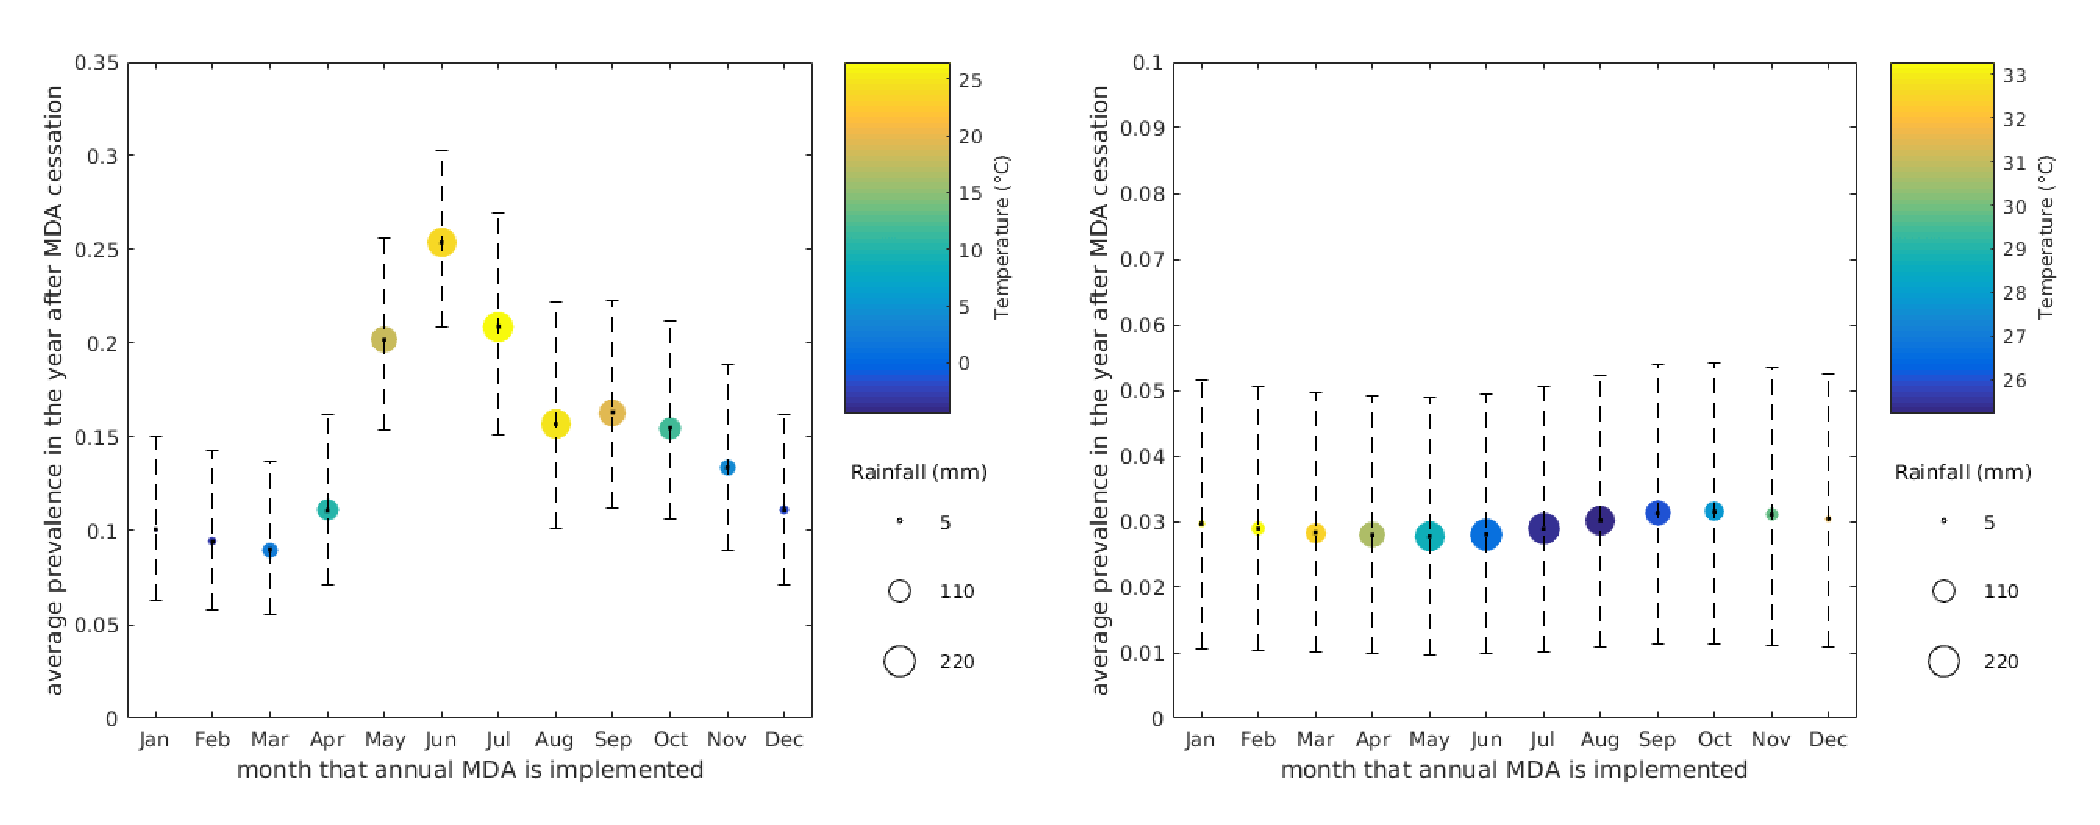
\includegraphics[height=6.0cm]{Project/Figures/STH/Fig8.pdf}
%\begin{adjustwidth}{-2.25in}{0in}$ % Comment out/remove adjustwidth environment if table fits in text column.
\caption{{\bf Seasonal MDA outcomes: Prevalence.}
Average prevalence (proportion of the population) across the 12 months following cessation of four annual MDA rounds for South Korea (left) and Nigeria (right). Depicted as best fit model averages with 95\% credible intervals.}
\label{Fig8}
%\end{adjustwidth}
\end{figure} 

\FloatBarrier

\section{Conclusions}

A deterministic macro-parasite model has been used to investigate known relationships between temperature, rainfall and \textit{A. lumbricoides} transmission. Model parameters were fitted to egg data from lab experiments, as well as prevalence data for two settings (South Korea 1977-78, Osun Province, Nigeria 2006-07) and used to predict the impact of these relationships on control strategies. Our results show that there could be large undetected fluctuations in the infective larval population, impacting transmission, without these effects being necessarily evident through untargeted surveys of human infection. 

In South Korea fitting resulted in a negative relationship between rainfall and transmission, with the higher rainfall in the summer months causing a steep decline in transmission rate. The temperate South Korean climate is expected to provide sufficient soil moisture for year-round egg development so it is plausible that low rainfall doesn't negatively impact the larval population. A transmission decrease due to high rainfall could be explained by the possibility eggs and larvae are being washed away through drainage systems, reducing host exposure to infection. 

Osun State is located in South-Western Nigeria, where rainfall is abundant across the year; there is no dry season, as experienced by the Northern areas of the country. The lack of dependency on rainfall displayed by fitting the model to data from this region indicates that the factors influencing disease dynamics differ from those in South Korea. The infection data is not seasonally structured, and hence gives only partial information on the seasonal trends, but the peak of infection in February does imply that there could be an additional level of seasonal variation that is not captured by the model. This could be indicative of seasonal changes in population behaviour or eating habits, or other climatic factors such as humidity and soil water-content.

There is also a large time period between the two studies, with almost 30 years between them (1978 to 2007), therefore effects seen in the earlier data set, from South Korea, may not be reflective of current transmission conditions. In particular, the rainfall dependency is fitted without any underlying explanatory mechanism, so if this effect is due to different behaviour between the dry and rainy seasons then cultural changes across the time period could have an impact this relationship. However, the relationships between infective stage development in the environment and temperature used in both the Nigeria and South Korea models are based on the same data source \cite{Wagner,Kim,Arene}, so I would expect this effect to be robust across the settings.

The model implies that optimal timing for MDA could coincide with minima in the environmental larval population, with the best treatment time predicted to be just preceding the annual upswing. These results agree with veterinary practices that advise treatment coinciding with hostile environmental conditions for the free-living stages, but we would expect a similar need for caution in this approach due to the potential for selecting for anthelmintic resistance \cite{Vercruysse}. For South Korea the much wider temperature range, as well as the inclusion of rainfall-influenced transmission in the model, led a predicted comparative decrease of 74.3\% in mean worm burden between the best and worst MDA timing. In comparison, the model predicted only a 12.8\% decrease for Nigeria. The climate data used was taken from as close a geographical location as possible to each study, although the monthly temperature averages used to fit these relationships will undoubtedly conceal daily fluctuations that would be expected to result in a more variable seasonal trend.

Analysis of these two contrasting settings demonstrates that the importance of seasonal factors for \textit{A. lumbricoides} control is expected to vary dramatically between different locations, depending on local climatic and transmission patterns. It is possible that different efficacies of treatment could lead to differences in the optimal time of year for treatment, or that changing the time of year between treatments could be beneficial in some settings. Frequency and number of MDA rounds could also impact our results, but benefits from treating at a seasonally optimal time of year are expected to be cumulative.

In temperate climates, like South Korea, high ranges of temperatures may allow for significant fluctuations in larval stage development across the year and could lead to important knock-on effects for MDA programs. Although the consistent temperature pattern in Nigeria results in low predicted seasonal differences and the data presented here shows no evidence for rainfall-dependence, it is possible that rainfall could still play an important role in other settings. Although current results are subject to further evidence, we can still use the findings to gain insight into the types of settings where we might expect seasonal effects that have the potential to impact the efficacy of MDA programs.

For example, the DeWorm3 trials, which aim to test the feasibility of interrupting the transmission of soil transmitted helminths (STH) using intensified MDA programs, are based in three countries with heterogeneous weather profiles: Benin, India and Malawi \cite{Deworm3}. In Benin the temperature range (monthly averages of 25-30\textdegree{C} \cite{TempB}) is narrower than that of Nigeria, so one would expect any seasonal drivers to be behavioural or rainfall-related. Temperatures are similarly high in Vellore, India, (monthly averages of 23-33\textdegree{C} \cite{TempV}) but with a steeper drop off in the cooler months that may introduce more seasonal variation. The third setting, Malawi, exhibits a fairly narrow but much lower temperature profile (monthly averages of 17-24\textdegree{C} \cite{TempM}) and, depending on rainfall effects, this is where we would expect seasonal MDA to have the highest impact due to the steep increase in maturation time as temperature drops under 20\textdegree{C}. Therefore in this setting it would be prudent to carefully consider the implications of seasonally-timed intensified MDA, as model results suggest that treatment during the cooler months could deliver maximum impact on \textit{A. lumbricoides} transmission.

All results are subject to uncertainty, through the Bayesian fitting framework, and under the assumptions made during model construction and selection. In addition, the egg survival data used to fit the model originates from experiments on \textit{Ascaris suum} life stages; there may still be some variation that has been unaccounted for, although previous studies have shown strong parallels between \textit{A. suum} and \textit{A. lumbricoides} eggs \cite{Boes}. Preferred epidemiological data would include more frequent measurements, with treatment at different times of the year in parallel communities across at least four years to provide greater insight into the long term infection dynamics. 

The model succeeds in qualitatively describing the biological components of the system and exhibits a good fit to both data sets, but caution must still be taken when interpreting predictions. Although the model is adapted from a well-established literature base there are still some limitations. For simplicity of calculation the helminth sex ratio within a host is not considered; infections consisting of only male or only female parasites should not result in any egg output. It has been demonstrated in previous studies that sexual reproduction in helminth infections can lead to a breakpoint in transmission, below which transmission is no longer viable \cite{Anderson1992,Anderson2017}. This breakpoint is likely to be highly dependent on setting-based factors, such as parasite aggregation and levels of human migration \cite{Hardwick2019}.

The assumed negative binomial relationship between mean worm burden and prevalence is also an approximation and not a true conversion. Additionally it could be worth considering the uncertainty around where transmission occurs; if infection is driven by hot-spots, such as community latrines, then these may have their own micro-climate that is less affected by the environmental conditions.

Taking seasonality into account when planning control programs can also be difficult; even in settings with clear seasonal trends there are likely to be additional complications when determining and successfully executing the optimal treatment timing. For example, the presence of other parasitic diseases in the human population could impact MDA outcomes and interfere with control measures; treatment often targets multiple STH infections and the best timing for one species may not be ideal for another. In addition, the logistics of treating at a particular time of year may be disproportionately costly or difficult for the benefits gained; it may be much easier to treat at particular times of year and moving MDA outside of these windows could result in lower coverage and hence worse overall outcomes.

If achievable, timing treatment to maximise impact now may create future problems further down the line; veterinary experience shows that timing MDA during low periods of larval density in the environment can magnify the risk of drug resistance by imposing additional selection pressures on the system.  Although anthelmintic resistance has not been definitively identified using currently available tools for human STH infections, it is still important to be cautious of any action that may encourage resistance to spread. Any seasonal recommendations for treatment timing should therefore be considered alongside the potential resistance development risk and further analysis would need to be done to inform any actions taken.

Nonetheless, our results suggest that variation in egg survival and maturation could be exploited to maximise the impact of MDA. Practically, we face the challenges of feasibility, caused by factors such as school term times and potential seasonal accessibility in hard-to-reach areas, but optimising treatment timing may be worth considering in some areas. Even though the evidence base in humans is weak there is enough grounds, combined with the depth of veterinary literature suggesting significant advantages to seasonally targeted anthelmintic therapy, to warrant further investigation.

\subsection{Chapter summary}

In this chapter I introduced STHs, focusing in particular on the global significance and biology of \textit{Ascaris lumbricoides}. I compiled and presented evidence for the impact temperature has on egg dynamics and used this to fit relationships between temperature and egg survival, development and viability. I also reviewed evidence for a relationship between rainfall and transmission and found this effect to be inconclusive. I then developed a novel seasonal model of transmission and treatment, incorporating the egg dynamics, and fitted this to data from South Korea and Nigeria, before predicting the impact of selective MDA timing across the year. My results show that for some settings, such as South Korea, optimising the time of year MDA is implemented across a program could lead to a comparative decrease of 74.5\% in mean worm days. However, in tropical settings where temperature variations are small, such as Nigeria, there is no evidence that MDA timing is important.

\chapter{Lymphatic filariasis elimination}
\chaptermark{LF elimination}
\label{chap:ELIM}

% Note: Talk to Joe about branching process literature review

\section{Introduction}

\subsection{Chapter Outline}

In this chapter I analyse the evidence for key biological determinants of lymphatic filariasis (LF) transmission and use a model of transmission derived from branching process theory to demonstrate that a target threshold of $<$1\% microfilariae (mf) prevalence is not likely to be sufficient for transmission interruption in communities with a mid-to-high annual biting rate. I also show that the insufficient and inconsistent experimental evidence behind key biological determinants of disease, particularly the transmission rate from vector to human, leads to high uncertainty in confidence of elimination success. This highlights the need for further experimental studies to refine our understanding of LF thresholds. I then go on to describe how local biting rate or vector density could be used as a proxy for transmission intensity to adapt targets between settings. 

\subsection{Disclaimer}

This chapter is adapted from my first author article entitled \textit{Evaluating the evidence for lymphatic filariasis elimination}, published in Trends in Parasitology in November 2019 \cite{Davis2019} and also from a general audience article \textit{Is there a worm on that branch?} published in a Biology and Medicine Special Issue of Mathematics Today in October 2019 \cite{Davis2019_MathsToday}. I was the first author on both articles and the work contained is my own, conducted with consultation from and collaboration with the other authors. There is some additional content and detail that was not included in these publications, specifically expansion and integration of relevant supplementary materials.

\subsection{Background}

The year 2019 marks a number of important anniversaries: 75 years since D-Day, 50 years since both the Stonewall riots and the first moon landing and 30 years since the fall of the Berlin Wall. It also marks 40 years since the global eradication of small pox -- the first infectious disease to be driven extinct by modern medicine \cite{Breman1980}. Prior to eradication, small pox had existed for at least 3,000 years and, with up to a 30\% mortality rate, was considered one of the most feared human diseases in the world \cite{Hopkins2002}. Now, thanks to a global vaccination campaign, the virus is believed to only exist in two secure laboratories and there have been no reported cases since 1978.

The success of the small pox programme led to an increase in discussions about eradication of other diseases, such as polio, mumps and guinea worm. In 1993, The Carter Center, a not-for-profit organisation founded in 1982 by former U.S. President Jimmy Carter, published a report declaring these three diseases, along with three others, as potentially eradicable with existing tools \cite{Klepac2015}. Malaria eradication, previously abandoned after being unsuccessfully targeted in the 1950s and 60s, also made a return to the global health agenda in 2008 \cite{Feachem2008}. Whilst the only other disease to join small pox in the last 40 years has been rinderpest, a livestock disease eradicated in 1999 \cite{Morens2011}, there has been some significant progress made towards achieving elimination across number of these diseases. Notably, global efforts have brought cases of Guinea worm down from almost 100,000 in 1993 to only 30, from just two countries, in 2017 \cite{Molyneux2017}.

LF was one of the diseases earmarked for eradication in 1993 \cite{Klepac2015}. Colloquially known as elephantiasis, LF is a mosquito-transmitted worm infection that can cause lasting and debilitating disability if left untreated \cite{WHOLF}. Although reliable written records of the disease only date back to the 16th century, historians argue it has been around for a lot longer. Due to the distinctive nature of some disease symptoms, such as the severe swelling of limbs, there are ancient artifacts dating all the way back to Pharaoh Mentuhotep II's reign over Ancient Egypt around 2000 BC that potentially provide evidence of filariasis in the ancient world \cite{Kenawy2015} (see Figure \ref{fig:Pharoh}). 

\begin{figure}
    \centering
    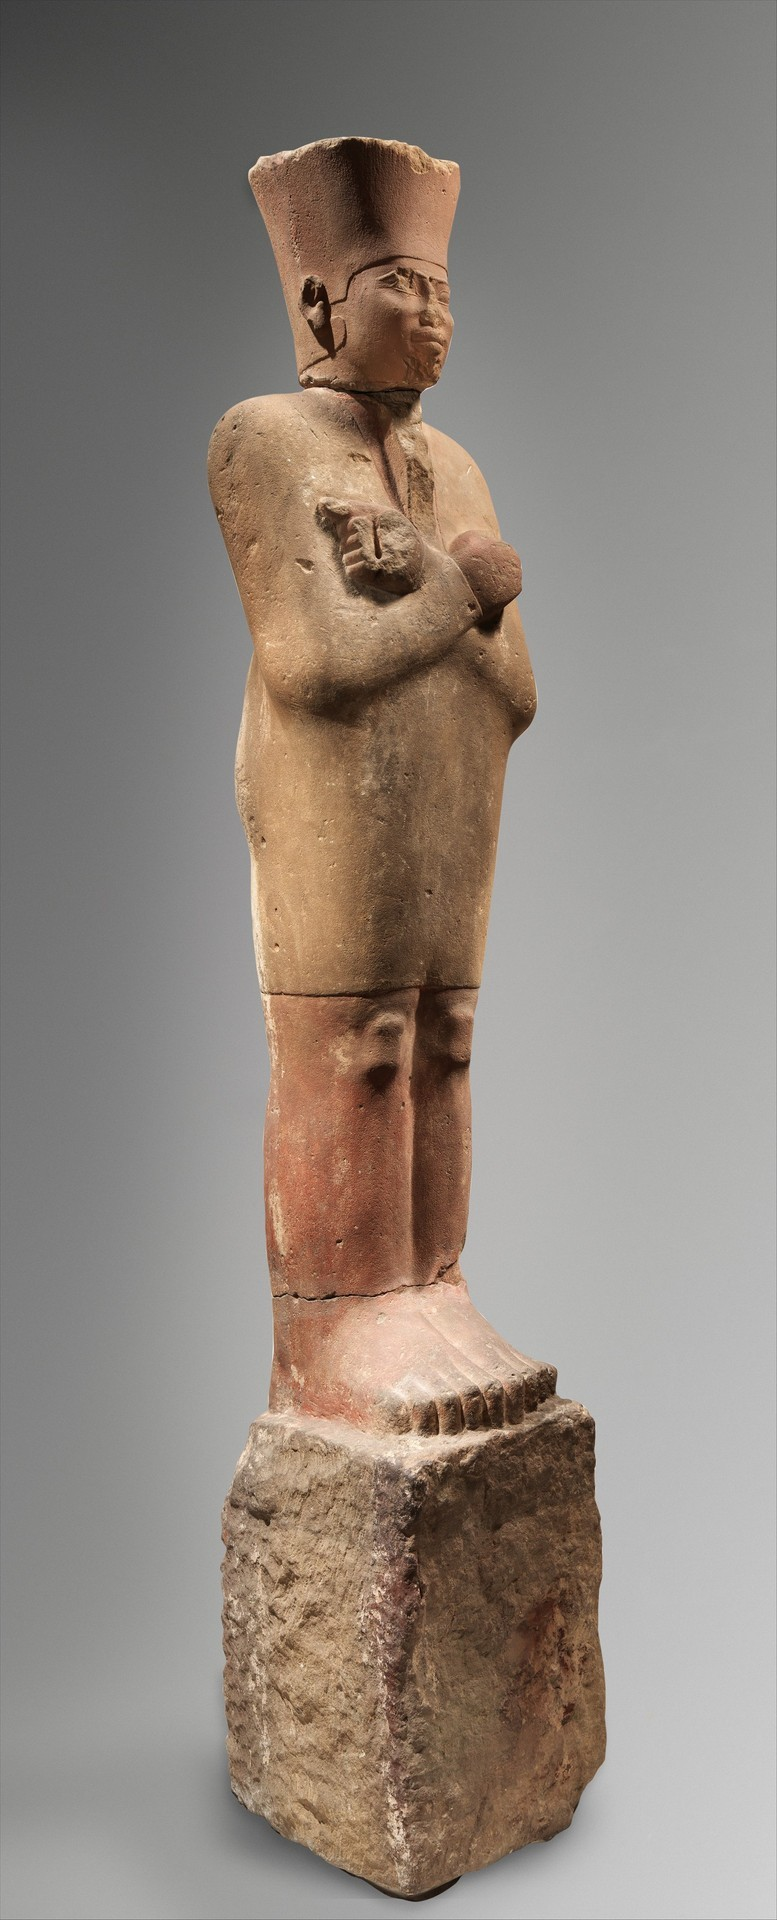
\includegraphics[height=15.3cm]{Project/Figures/LFElimination/Mentuhotep.jpg}
    \caption{A statue of Pharoah Mentuhotep  II (who reigned c. 2055--2004 BC). Swollen limbs, as are depicted here in the legs, are a characteristic symptom of lymphatic filariasis. Image credit: Statue of Nebhepetre Mentuhotep II in the Jubilee Garment MET DP302395.jpg by Pharos / Wikimedia Commons / CC0 1.0}
    \label{fig:Pharoh}
\end{figure}

Four-thousand years later, in AD 2000, infection was still widespread across tropical regions, with 120 million people estimated to be at risk \cite{Melrose2004}. Due to over 7 billion treatments being delivered through mass drug administrations (MDA, where large proportions of the population are treated at the same time, usually yearly), the number of infected people is thought to have lowered substantially since the millennium, with fourteen countries having been validated as reaching less than 1\% prevalence across their endemic regions \cite{WHOLF,WHOWER}. 

The question which now faces the Global Programme to Eliminate Lymphatic Filariasis (GPELF), is whether and where LF is likely to be eliminated once this low level of infection is achieved. The mathematical literature on infectious diseases has been crucial in informing the discussion on eliminating infections, and a number of challenges remain \cite{Klepac2015}. Here we address the particular challenges of modelling the elimination of a sexually reproducing parasite which is transmitted by a mosquito.

\subsection[Global situation]{Global situation and progress}

There are currently 886 million people across 52 countries worldwide at risk of LF \cite{WHO2019_FactSheet}. Infection is caused by a mosquito-transmitted filarial worm and, if left untreated, can lead to permanent and debilitating disability. GPELF set a target of elimination as a public health problem (EPHP, see Glossary) in 1997, leading to over 7.1 billion treatments delivered as part of mass drug administrations (MDA) since 2000 \cite{WHO2017_GPELF}. In 2011, the WHO published guidelines for halting treatment and verifying EPHP through the use of Transmission Assessment Surveys (TAS) to measure a target threshold \cite{WHO2017_Validation,WHO2017_Alternatives}. By October 2018, 14 countries had reached this target, and 554 million people worldwide no longer require mass treatments \cite{WHO2019_FactSheet}.

As indicated by the name of the TAS, it was hoped that reaching these targets would lead to elimination of transmission (EOT) in most areas. However, in Sri Lanka the TAS has been demonstrated as not sensitive enough to detect low-level persistence \cite{rao2014,rebollo2015} and pockets of transmission are still being found despite EPHP validation. The community is now revisiting the TAS methods, including the original target of 1\% microfilaria (mf) prevalence \cite{WHO2016}, particularly in the context of the new triple-drug regimen which is hoped to accelerate progress, but will require different post-treatment surveillance \cite{Irvine2017_Tripledrug}.

It is possible that achieving EPHP, according to the current definition, will lead to EOT in some settings \cite{DeJian2013,Won2018}, but the high levels of variability between localities and uncertainty in our knowledge of transmission makes it hard to predict where this will occur. This is exacerbated further by seasonal variation in environmental conditions, which has been shown to impact a number of helminth infections \cite{Davis2018,White2011}. Residual infection remaining after MDA cessation can lead to resurgence and reintroduction \cite{Xu2019,Singh2015}, with long-term persistence dependent on a range of factors \cite{Minetti2019}.

\section{Methods}

\subsection[Elimination theory]{Sexual reproduction in the host and elimination}

The sexual reproduction of filarial worms requires both male and female parasites to be present in an individual host for microfilariae production, so at a sufficiently low prevalence we would expect most infections to be non-transmissible due to low parasite load (i.e. a low probability of male and female adults in the same host). This is expected to result in fewer onward infections, and hence increasingly lower prevalence and intensity, until infection dies out. The threshold below which we expect this phenomenon to occur is called the breakpoint \cite{Anderson1992,Anderson2017}. As the focus of some NTD programs has shifted from control towards elimination, there have been a number of studies aiming to quantify these thresholds for a variety of helminth infections within the NTD umbrella \cite{Truscott2017,Irvine2018,Klepac2015,Hollingsworth2015}.

\begin{figure}
    \centering
    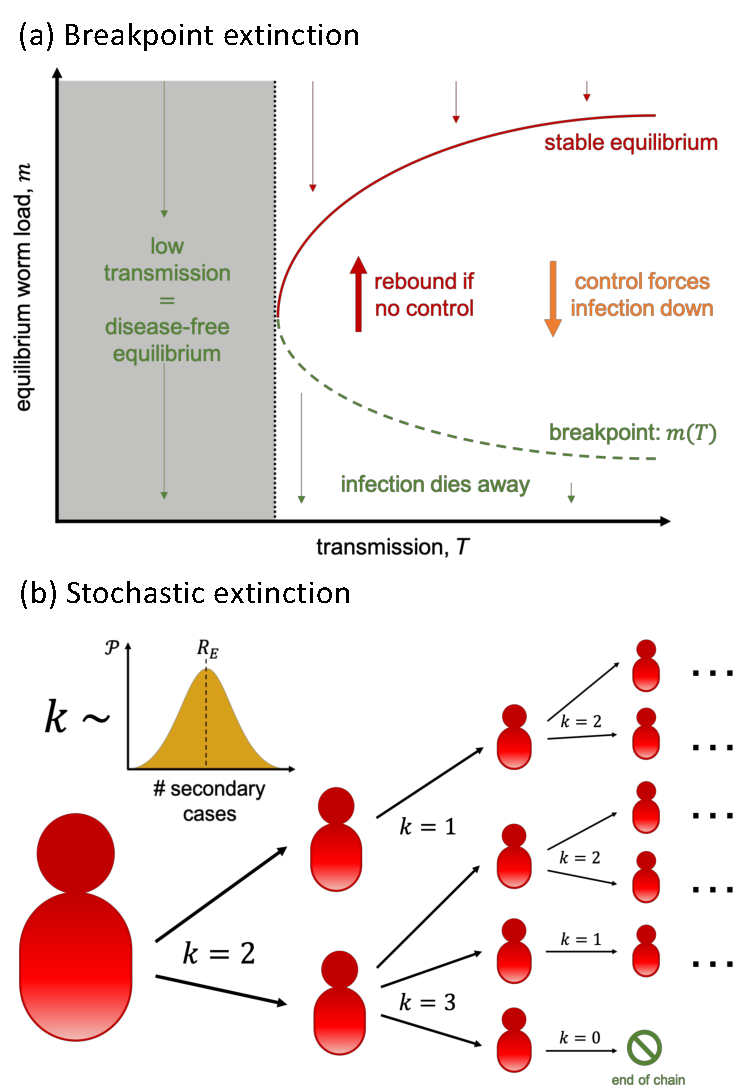
\includegraphics[height=15.3cm]{Project/Figures/LFElimination/Figure1.pdf}
    \caption{LF extinction theory. Schematics comparing the theory behind breakpoint extinction (a) and stochastic extinction (b) for LF. (a) For sufficiently low transmission intensities (i.e. low biting rates) disease levels will drop away to zero. Beyond the critical transmission level (black dotted line) there are three equilibria: high disease (stable, red), low disease (unstable “breakpoint”, green), disease-free (stable, black). Disease levels above the breakpoint will increase to the higher equilibrium, whereas disease levels below will decrease to zero. (b) Visual depiction of a transmission chain starting with one infectious individual. The number of secondary infections caused by each currently infectious individual are sampled from the secondary case distribution. This is used to simulate the onward chains of infection; extinction occurs when all chains die out (i.e. have no secondary cases). Stochastic variation can cause this to occur even above the theoretical breakpoint threshold.}
    \label{fig:Elim_1}
\end{figure}

This theory has certain consequences for control (Figure \ref{fig:Elim_1}a). If transmission is sufficiently low, then the infection is expected to die out. If there is a higher transmission rate, outcomes depend on the mean worm load in the population; if, usually through control strategies, the worm load is below the green dashed line (the breakpoint) then elimination is assured. Previous modelling studies that have assessed breakpoint thresholds have found values of much less than 1\% mf prevalence \cite{Singh2015,Michael2017,Michael2018,Gambhir2010}. It has been previously demonstrated that factors such as parasite aggregation and vector competence will further affect these thresholds \cite{irvine2015} and the majority of studies have focused on specific geographical areas, resulting in a wide range of suggested breakpoints across the literature.

Measuring breakpoints that are substantially lower than 1\% mf prevalence would require infeasible sample sizes and survey costs. In this review we don’t argue for a specific breakpoint, instead focusing on asserting that the experimental evidence is too uncertain to conclusively support a 1\% threshold and emphasizing the importance of spatial heterogeneity.

Whilst breakpoint theory is extremely useful, it is also possible for stochastic, or chance, extinction to occur before this break-point is reached, particularly when infection levels are low (Figure \ref{fig:Elim_1}b). The probability of elimination, given a particular prevalence (e.g. 1\%), can be calculated by considering the probability a chain of transmission will die out (this chain has similarities to a branching process \cite{Watson1875}). These types of branching-process-style methods have been used for soil-transmitted helminths \cite{Cornell2004_Stochastic,Cornell2004_Ultimate}, but have been adapted here to account for vector-borne transmission with an aggregated bite risk \cite{Fowler2016,Irvine2017_Mosquitobite}

Current guidelines mean EPHP is validated after passing TAS, but we have little experience in what this means for long-term transmission. Assuming for simplicity that TAS is able to measure a true mf prevalence of less than 1\%, this theory of stochastic extinction can be used to estimate how the future probability of EOT (zero infections) depends on a range of setting- and disease-specific variables. This process uses the distribution of the number of infectious secondary cases caused by one infectious individual, the mean of which is the effective reproductive number ($R_e$).

\begin{figure}
    \centering
    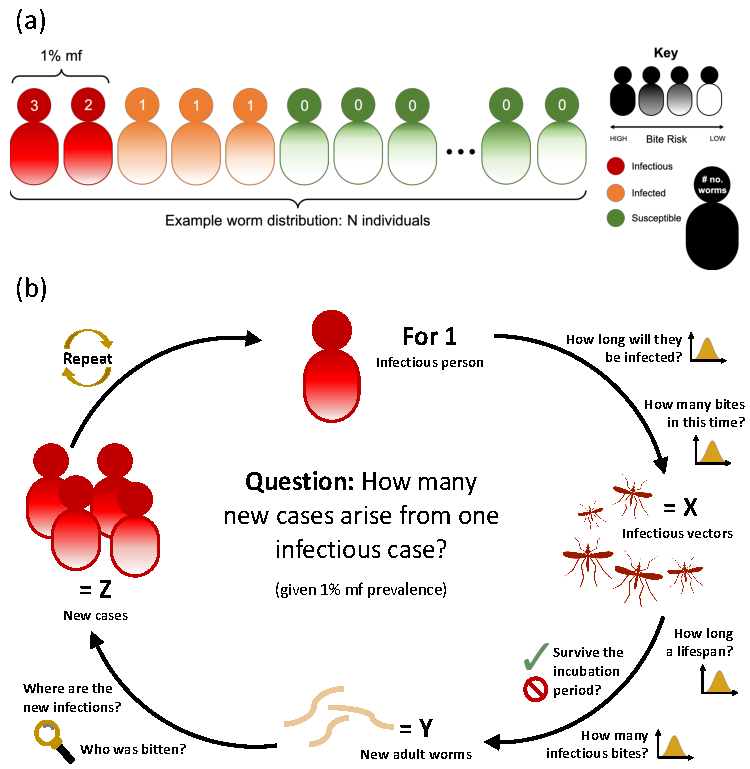
\includegraphics{Project/Figures/LFElimination/Figure2.pdf}
    \caption{Simulating transmission chain extinction. A schematic describing the simulation process for calculating the number of secondary cases produced by one infectious individual in a population with 1\% mf prevalence. (a) Allocate distribution of adult worms and bite risks across the population. Individuals with 1 worm are infected but not infectious, individuals with ≥2 worms are considered potentially infectious. (b) Generational calculation of number of new infectious cases caused by aan average infectious individual. One infectious individual infects $X$ vectors. The vectors that survive the incubation take infectious blood meals, resulting in $Y$ new adult worms. These worms are distributed across the population according to bite risk aggregation, resulting in $Z$ new infectious ($\geq$2 worms) individuals.}
    \label{fig:Elim_2}
\end{figure}

As a toy example, for a population of 1000 and 1\% mf prevalence, we consider a distribution of individual worm burdens (Figure \ref{fig:Elim_2}a). Infections with only one worm are non-transmissible. From one infectious person you then get the number of new cases, $Z$, caused during their infectious period (Figure \ref{fig:Elim_2}b). Since transmission represents a chance event, $Z$ is best represented by a distribution, and acts as a proxy for $R_e$. This distribution determines the probability of the transmission chain dying out, i.e. no further cases, at some point in the future. We use this to give a univariate demonstration of the present parameter uncertainty and how this might impact two epidemiological measures: the probability of elimination and the effective reproductive number.

\subsection[Branching processes]{Branching process extinction}
The most common branching process formulation is the Galton-Watson process \cite{Watson1875}, which we outline here before adapting for LF (Figure 3, right):

Let $X_n$ denote the number of infectious individuals in generation $n$ and for each infectious individual, $i$, let $Z_{n,i}$ be the number of new infectious cases directly caused by that individual. $Z_{n,i}$ iid random variables over $n\in{0,1,2...}$ and $i\in{1,...,X_n}$.

Assuming we start a chain of infection with one infectious individual, $X_0=1$, we then have the recurrence equation,
\begin{equation}
    X_{n+1} = \sum_{i=1}^{X_n}Z_{n,i}\,.
\end{equation}

The extinction probability of one chain of infection is the probability that $X_n=0$ for some $n>0$, or that $\lim_{n\rightarrow\infty}P[X_n=0]$.

Define $p_m$ ($m=0,1,2,...$) as the probability of an individual producing $m$ offspring and $d_m$ as the probability of extinction by the $m$th generation; $d_0=0$ as we start with one individual in generation $0$. Hence $d_m$ is an increasing, bounded sequence ($0=d_m\leq d_1\leq d_2\leq ... \leq 1$) and therefore converges to some limit, $d$, where $0\leq d\leq 1$ is the ultimate extinction probability.

\begin{eqnarray}
    d_1 &=& p_0 \\
    d_2 &=& p_0 + \sum_{j=1}p_j(d_1)^j\\
    &...&\\
    d_m &=& p_0 +  \sum_{j=1}p_j(d_{m-1})^j \,.
\end{eqnarray}

We can write this as,

\begin{equation}
    d_m = f(d_{m-1})
\end{equation}
where $f$ is the ordinary generating function:
\begin{equation}
   f(d) = p_0 +  \sum_{j=1}p_jd^j \,.
\end{equation}

Since $d_m\rightarrow d$, we can find the probability of ultimate extinction by solving $d=h(d)$. 

We want to show that $d$ is the smallest non-negative root of this equation. Take $b>0$ also a root with $b\neq d$ and $b=f(b)$, then we have that $d_1=f(0)\leq f(b)=b$, hence $d_1\leq b$. Assume $d_k\leq b$ for some $k$, then

\begin{equation}
    d_{k+1} = f(d_k) \leq f(b) = b \,,
\end{equation}

since $f$ is an increasing function. Hence, by induction $d$ is the smallest non-negative root. The function, $f$, is also convex and hence has at most two real roots. Since one is always a root, $f(1)=\sum_{j=0}p_j=1$, then the probability of ultimate extinction is only less than one if the second root both exists and lies between zero and one. 

By considering the gradient of $f$ at one, $f'(1) = \sum_{j=1}jp_j$, we can determine the location of the other root -- namely there is only a second root in $[0,1]$ if $f'(1)>1$. Notably this gradient, $f'(1)$, is equal to the average number of secondary cases caused by a single infectious individual, often called the basic reproduction number to describe early outbreak dynamics. Since we are considering a situation where there is a background population prevalence that has been artificially lowered to 1\%, we call this the effective reproduction number, $R_e$.

In our model (further details below), we want to take account of the heterogeneous worm distribution across hosts, as it is a key feature of the system. Therefore, it is not possible to directly calculate either the effective reproduction number or the probability of extinction, but both can be calculated numerically by considering the outcome distributions of stochastic simulations. In particular, by calculating the proportion of simulated individual infections that result in each number of onward infections, we can generate a discrete numerical approximation of our secondary case offspring probability distribution. 

From this, we can iterate through each generation to find the probability that extinction has occurred. This probability converges over time and, if sufficient generations are considered, can be used as an approximation of the ultimate extinction probability, $d$.

\subsection[LF model]{Lymphatic filariasis model}
In order to estimate the extinction probability for LF, we simulate a population of 1000 individuals, with variable infection risk, of whom 1\% are productively infected (producing transmissible offspring, mf), a proportion are unproductively infected and the remainder are uninfected. We assume the dominant vector is \textit{Anopheles gambiae}. 

We then calculate for a randomly infected individual, the number of onward productive infections they produce according a model of the life-cycle. An infection lasts for a randomly selected period of time (exponential, mean $1/r$, the estimated fecund life span, 6 years). This individual has a risk of being bitten relative to the rest of the population (Gamma, mean=1), which, depending on the annual bite rate (ABR), or the expected number of bites per year, generates the expected number of bites in during their infectious period. For each bite, there is a probability, $c$, that the mosquito becomes infected. We assume each new infection occurs in a new mosquito, which gives an upper bound of the total number of infected mosquitoes for this individual.

Each mosquito then has exponentially distributed life expectancy (mean$=1/g$, 6.9 days \cite{Killeen2000,Subramanian1998}) and has to survive an incubation period (also Exponential, mean$=\nu$, 8.5 days \cite{erickson2009}). From this we can derive the probability a vector survives to infectiousness and, using a binomial distribution, calculate the total number of infected vectors, $V$, which survive the incubation period. The number of infectious bites caused by these vectors is then Poisson distributed at a daily rate, $f$=0.335 \cite{Subramanian1998}, per vector and of these bites only a small proportion, $b\ll1$ \cite{Hairston1968,Jones2014}, will successfully lead to a productive infection. The efficacy of transmission from vector to host is so low due to the route the larvae must take to establish; rather than being injected into the bloodstream during the bite, the larvae must instead independently fall onto the skin and find the hole left by the mosquito after feeding.

This describes the number of new adult worms $Y$, that are established in humans resulting from the entire duration of this one individual's infection (one distinct outcome per iteration, creating a distribution). From the total number of new adult worms, $Y$, we can derive the effect on prevalence by sampling $Y$ individuals, with replacement, according to bite risk. Each time an individual is sampled they gain 1 adult worm. We then compare new worm burdens with previous worm burdens -- how many new infectious ($\geq 2$ worms) cases are there that were previously not infectious ($\leq 1$ worm)? This gives our number of secondary infections, $Z$.

Then the mean number of new infectious humans is $R_e$, which here relates to the full-cycle reproduction number focusing on human infections only. If $R_e<1$ then eventual extinction will occur -- implying that prevalence is already below the theoretical breakpoint of the system. However, if $R_e>1$ then extinction is not guaranteed but may still occur. We need to consider the offspring distribution of the transmission chain, $p_j$ probability of having $j$ secondary cases, which can be approximated by the scaled frequency of secondary infectious case counts, in order to calculate the probability of extinction.

\section[Life-cycle variables]{Empirical evidence for life-cycle variables}

We now review evidence for key parameters in the life-cycle which drive transmission (Figure \ref{fig:Elim_3}). As previously mentioned, a number of these variables, such as the annual biting rate (ABR), are likely to introduce large differences due to the high spatial variability. Others, such as the probability an infectious mosquito bite results in a viable human infection, have the potential to be more consistent across settings, but currently lack in experimental evidence. Table \ref{tab:Elim} at the end of this section outlines the range of values for biological variables found in the literature. 

\begin{figure}
    \centering
    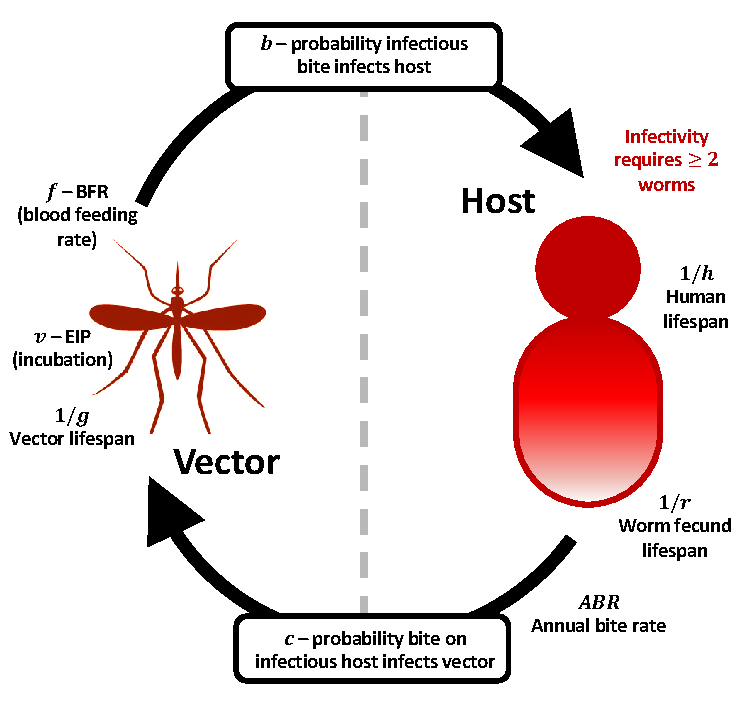
\includegraphics{Project/Figures/LFElimination/Figure3.pdf}
    \caption{LF life-cycle. Life-cycle schematic demonstrating key biological variables that could affect prediction of elimination success. Duration of infection is determined by human and fecund worm lifespans. Infection from host to vector depends on the annual biting rate (ABR) and the probability a bite on an infectious host infects a vector. The number of vectors that survive to infectivity depends on incubation (EIP) and vector lifespan. Transmission from vector to host is then determined by the blood feeding rate and the probability an infectious bite results in a viable adult infection, as well as the requirement for $\geq$2 worms for infectivity.}
    \label{fig:Elim_3}
\end{figure}

A detailed literature review turns up widely varying estimates of ABR, partially due to geographical variation. These values, from countries with history of LF endemicity, range from 3 \cite{Killeen2000} to 611 \cite{Michael2016} bites per person per day. A number of these are based on human landing catches \cite{Killeen2000,Michael2016,Braack2015}, with the majority relying on studies from the 1960s and 70s \cite{Michael2016}, whilst some are derived from models \cite{Stolk2005}. Despite a wealth of historic studies, supported by the malaria literature (which covers many of the same vector species including \textit{Anopheles gambiae}), human landing catches are often considered unethical and give highly variable results. Relying on historic estimates can also disregard changes in socio-economic conditions resulting in decreased vector-human contact.

Current estimates in the literature of the basic reproductive number without control, $R_0$, range from 0-2.5 \cite{Stone2014}, depending on the vector-host ratio (an alternative metric to ABR). Although setting-specific values of $R_0$ for other diseases can often be calculated from infection data, the global landscape of public health history for LF means that we have very little contemporary baseline (pre-control) data with which to do this. As an alternative, we can consider the previously mentioned estimation of $R_e$.

Another important, but largely uncertain, factor is the degree of parasite aggregation, measured inversely by the negative binomial $k$. For LF, adult worm aggregation is considered to be driven by heterogeneous transmission, caused by host variation in bite risk \cite{Irvine2018}. Initial estimates for $k$ were based on mf data ($k$ = 0.08, 0.3 \cite{irvine2015,Irvine2017_Mosquitobite}). However, a recent study in Papua New Guinea used bite and mf data to demonstrate that the $k$ for bite risk is an order of magnitude larger than that for mf aggregation, giving a refined estimate of 0.73 (s.d. 0.035), with site-specific estimates ranging from 0.3--1.3 [15, 26]. We will now separate transmission into two parts: humans to mosquitoes, and mosquitoes to humans. When considering the former the key variables are duration of infection, which depends on fecund worm lifespan, and the probability that a vector biting an infected host will become infectious. 

Often worm lifespan is stated as being 6-8 \cite{WHO2019_FactSheet} or 5-10 years \cite{Norman2000_epifil,Stolk2006}, but reference trails rarely reveal empirical evidence. There are studies that corroborate similar ranges, such as 2.1-5.4 \cite{Vanamail1996} or 9.1-11.8 \cite{Subramanian2004} years, but there are also estimates in the literature of up to 40 years \cite{Carme1979}.

Infectivity to mosquitoes depends on mf intensity, leading to wide ranges of 15-60\% of vectors becoming infected from a single mf positive bite \cite{Subramanian1998,gambhir2008}.

Infection from vector to human is governed by the number of infectious bloodmeals one mosquito will take – calculated from vector survival and competence, extrinsic incubation period (EIR) and blood feeding rate (BFR) – and the probability one infectious bite will result in a viable infection. There are reasonable estimates for vector survival and BFR from the malaria literature \cite{Killeen2000,Gary2001} and for LF incubation \cite{erickson2009}, although these do not typically account for the impact of infection on survival \cite{Subramanian1998}. 

One key parameter of infection, the probability an infectious bite results in a mature human infection, is largely unknown. Estimates range from 10-5 to 10-3 \cite{Hairston1968,Jones2014} and are usually broken down into three steps: the L3 leaving the vector, entering the host and developing to fecundity. The first is relatively straightforward to measure \cite{deMeillon1997}, although poses ethical issues, and the second can be estimated using mouse models \cite{Ho1967,Ewert1967}. The third is harder; best estimates are calculated by using \textit{Brugia malayi} studies to derive a daily death rate and then applying this across the longer \textit{Wucheria bancrofti} developmental period \cite{Norman2000_epifil,Addiss2000}. Although \textit{Brugia malayi} is also a cause of LF in humans, the parasite is of a separate species to \textit{Wucheria spp.} and hence is not necessarily comparable in this way. 

\begin{sidewaystable}[p]
    \centering
    \begin{tabular}{|l|p{70mm}|p{95mm}|1|}
    \hline
    \multicolumn{1}{|l|}{\bf Item} & \multicolumn{1}{|l|}{\bf Biological meaning} &
\multicolumn{1}{|l|}{\bf Range of estimates} &
\multicolumn{1}{|l|}{\bf Mid-point} \\ \hline
        $\psi_1$ & Prop L3 leave vector per bite & 0.437(\textbf{0.363 -- 0.511})\cite{deMeillon1997}, 0.414 \cite{deMeillon1997} & 0.437  \\
        $psi_2$ & Prop L3 enter host & 0.223 \cite{Norman2000_epifil,Ewert1967} & 0.223 \\
        $w$ & Developmental period in host & \textbf{6 months 9 days -- 12 months 14 days} \cite{Addiss2000}, 8 months 4 days \cite{Hairston1968} & \\
        $s_2$ & Prop L3 develop to adulthood & (\textbf{0.036 -- 5.68})$\times 10^{-3}$ \cite{Hairston1968,gambhir2008,erickson2009,Jones2014} & 0.437$\times 10^{-3}$ \\
        $b$ & Probability infectious bite infects human & $=\psi_1\psi_2 s_2$ = (\textbf{0.15 -- 9.29})$\times 10^{-4}$, 1/47$\times 10^{-3}$ \cite{Hairston1968,Jones2014} & 1.43$\times 10^{-4}$ \\
        $ABR$ & Annual biting rate & \textbf{1129} \cite{Killeen2000}, 1500 \cite{Michael2016}, 22320 \cite{Braack2015}, 24090 \cite{Killeen2000}, 26400 \cite{Stolk2005}, 41975 \cite{Braack2015}, \textbf{69120} \cite{Stolk2005}, 223000 \cite{Michael2016} & 24090 \\
        $1/g$ & Vector life span (days) & \textbf{5.4 -- 9.5} \cite{Killeen2000,Subramanian1998} & 6.86 \\
        $1/r$ & Worm fecund life span (years) & \textbf{2.1} \cite{Vanamail1996}, 5.4 \cite{Vanamail1996}, 9.1 \cite{Subramanian2004}, \textbf{11.8} \cite{Subramanian2004}, 40 \cite{Carme1979} & 6 \\
        $c$ & Probability infectious bite infects vector & 0.37 \cite{gambhir2008} (\textbf{0.15--0.6}) \cite{Subramanian1998} & 0.37 \\
        $v$ & Extrinsic incubation period (days) & \textbf{7 -- 10} \cite{erickson2009} & 8.5 \\
        $f$ & Daily vector blood feeding rate & \textbf{0.26 -- 0.41} \cite{Subramanian1998} & 0.335 \\
        $k$ & Parasite aggregation & \textbf{0.08 -- 1} [various] & 0.5 \\
        \hline
    \end{tabular}
    \caption{Values for biological variables found in the literature, which were used in the calculation of results shown in Figure \ref{fig:Elim_4}. Values taken as maximum and minimum estimates for analysis are indicated in bold and mid-value estimates are listed separately. Mid-value estimates that are not also listed in the “Range of estimates” column are chosen to represent a mid-ground, usually an average of the maximum and minimum values.}
    \label{tab:Elim}
\end{sidewaystable}

\section[Results]{Results}

\begin{figure}
    \centering
    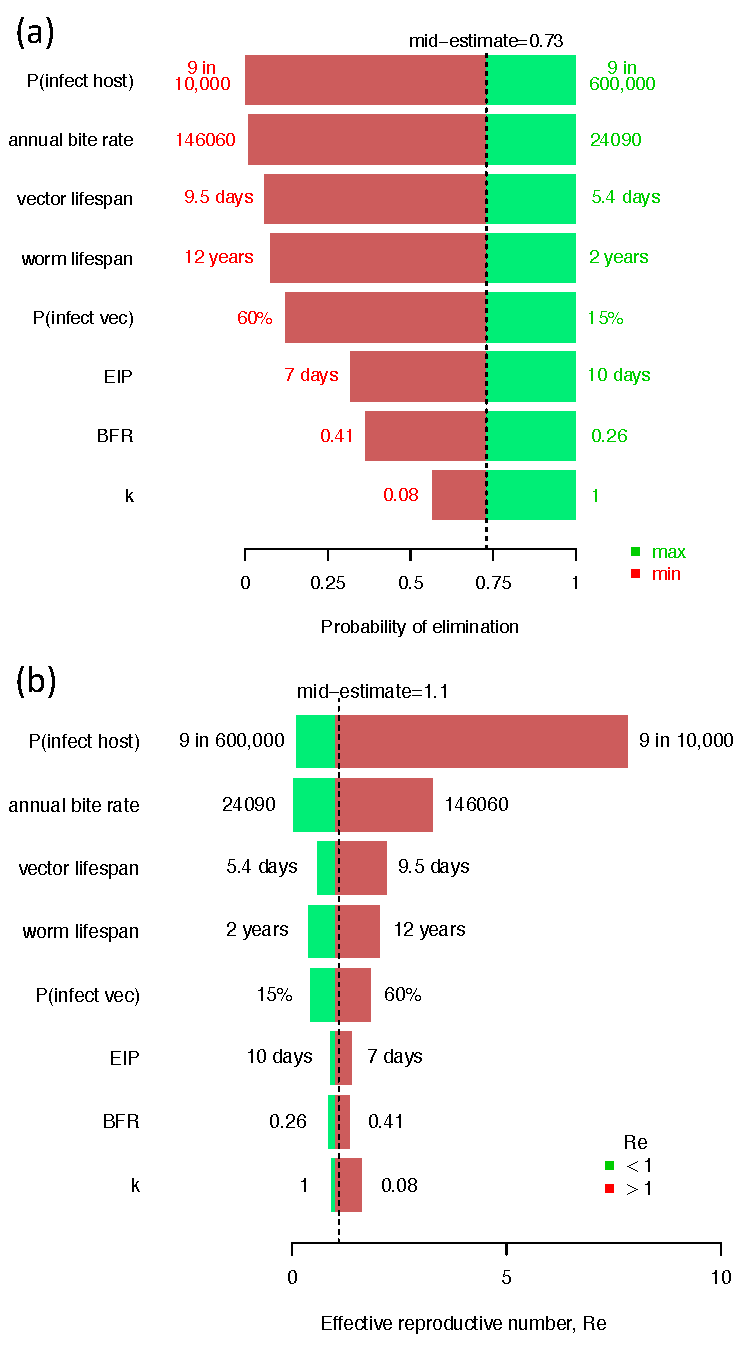
\includegraphics[height=16cm]{Project/Figures/LFElimination/Figure4.pdf}
    \caption{Predicting elimination probabilities. Illustration of the potential impact of high uncertainty in variables by considering their univariate impact on the probability of elimination (a) and the effective reproductive number (b) for the key biological variables of the LF transmission cycle. Assuming an mf prevalence of 1\% and a human population size of 1000. References for ranges of variables considered can be found in Table \ref{tab:Elim}. Note that this univariate analysis should be interpreted carefully as variables are likely to be correlated in ways which we cannot yet account for. For example, the mid-estimates here have been chosen to represent a mid-ground of ranges found in the literature and are not necessarily representative of the true values or ranges that may exist across real-world settings.}
    \label{fig:Elim_4}
\end{figure}

If we include these parameters in the simple framework described above, we can see how the uncertainty affects our estimates of key epidemiological measures (Figure \ref{fig:Elim_4}). The mid-points of elimination probability (0.73) and $R_e$ (1.1) are not intended to be true estimates, rather they represent a mid-ground of the parameter ranges found in the literature and a basis for comparison. 

The variable which generates the most univariate uncertainty is the probability an infectious mosquito bite will infect a human, $b$, due to the wide range of possible values. Variation in elimination probability due to ABR, which is correlated with the basic reproductive number ($R_0$), is also very high. This is due to both measurement inaccuracy and spatiotemporal variability. Parameters that are known to be key drivers in the probability of elimination, worm fecund lifespan and the degree of adult worm aggregation \cite{irvine2015,Truscott2017,Anderson2014}, potentially induce lower uncertainty here due to considering narrower plausible intervals.

In addition to the probability of elimination, we also consider the effective reproductive number, $R_e$. It is important to note that for helminth infections, metrics often refer to the number of adult filarial worms arising from one adult filarial worm, rather than considering human infections. However, the theory is similar enough to allow heuristic comparison. Our mid-estimate for $R_e$ is chosen to be close to 1, representative of the low-level transmission observed in some post-MDA settings, but varying the probability an infectious mosquito bite will lead to a patent infection ($b$) can lead to an order of magnitude difference. In fact, it is possible to push the estimate of $R_e$ across the critical threshold ($R_e=1$) between extinction and endemicity by adjusting any variable within the ranges found in the literature. This reinforces the importance of using reliable variable estimates when making predictions, particularly in elimination settings where infection data are sparse. 

We can characterise the probability of extinction from achievement of 1\% mf prevalence in relation to transmission intensity (Figure \ref{fig:Elim_5}, orange curve). When the annual biting rate (ABR) is low, then infection is highly likely to fade out, but this probability declines as the biting rate increases. This emphasises the importance of local context in determining the extinction probability from this endpoint. We additionally simulated the curve for a halving of the endpoint - a prevalence of 0.5\%. This, of course, increases the probability of extinction, but would require much larger sample sizes to evaluate. 

\begin{figure}
    \centering
    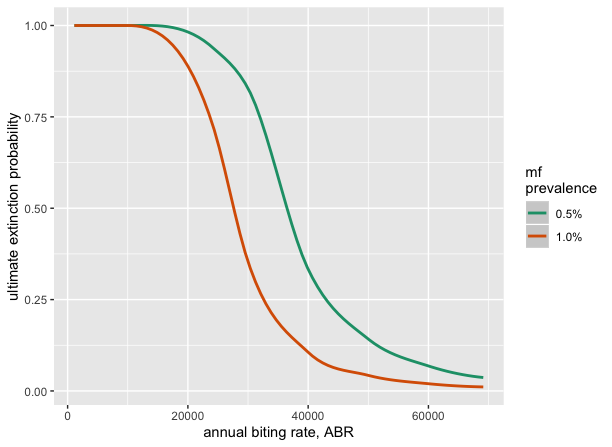
\includegraphics[height=10cm]{Project/Figures/LFElimination/Figure5.png}
    \caption{The probability that transmission will become extinct for different annual biting rates (ABR) and different starting prevalence (green 0.5\%, orange 1\%).  At low biting rates, the infection is highly likely to fade out, but for high biting rates it is unlikely.}
    \label{fig:Elim_5}
\end{figure}

\section{Recommendations}

Due to the demonstrated uncertainty that knowledge gaps, particularly in the establishment of a patent infection, can cause in estimating elimination thresholds it would be prudent to refine the evidence for these variables. Here we discuss a few options for future studies and analyses that we believe could strengthen the knowledge base.

The probability that an infectious bite leads to an infectious host cannot be measured experimentally in humans, however we can improve current estimates with anecdotal and observational studies. Longitudinal studies can provide evidence of the time to antigen positivity and the time to mf positivity in children, or in adults that have moved from non-endemic to endemic regions. One existing study, looking at acquisition in travellers, surmises that the majority of cases are in individuals who spent in excess of six months in an endemic region [49], whereas another cites a number of travellers contracting infection with only one month of exposure \cite{Jones2014}. Entomological studies routinely estimate ABR through human landing catch data, and individual exposure can be quantified based on net usage and vector biting habits \cite{Reimer2013_insecticidal,Thomsen2017}.

The range of ABRs discussed are very broad estimates, covering a wide range of settings, but this can be a difficult variable to measure consistently. It may be possible to obtain greater certainty in $R_e$ without accurate ABR measures for each location. For example, estimates of low, medium or high vector densities would still improve our predictions and these categories of exposure, which act as a proxy for $R_0$ classification, could be informed by a combination of trap densities and vector control coverage. Spatial heterogeneity can also occur within implementation units, posing problems for any categorisation process, so it is important that treatment targets are determined by the maximum transmission measure for a region. 

We have used basic analyses to highlight that the existing experimental evidence does not afford a high degree of certainty at the current 1\% mf prevalence elimination threshold. This is mainly because of uncertainties in variables which could be either experimentally or analytically refined, but also due to spatiotemporal variation in vector densities and biting rates \cite{Michael2016}. That varying the value of one input variable within sensible ranges found in the literature can make such an impact on predictions, demonstrates the difficulties posed by targeting EOT when we know local heterogeneities and variability are difficult to measure. Observations of ongoing transmission in parts of validated countries offer empirical support to our concerns with the EPHP target, prompting some important outstanding policy questions. This highlights the need for both refinement of the experimental evidence based and care when selecting model parameters from the literature.

Recent empirical evidence suggests the current survey does not capture ongoing transmission. By altering the survey design, through different diagnostics, measuring mosquitoes or sampling on a more detailed spatial scale, it is possible that areas of high transmission rates could be picked up earlier. In order to support efforts to eliminate lymphatic filariasis we would recommend a multi-pronged approach: improving the experimental evidence base of measurable quantities; detailed analysis of existing infection data to improve our understanding of the infection risk associated with an infectious bite; and development of a discrete system to classify vector density, as a proxy for transmission intensity, to allow comparison of different regions. The optimisation of elimination program strategies and surveillance will require continual revisiting of predictions as we gather more epidemiological data through existing surveys and monitoring infrastructures, as well as expanded epidemiological and surveillance studies at low prevalence. 

As more countries cease interventions and move to post-validation surveillance it is increasingly obvious that transmission breakpoints are unlikely to be one-size-fits-all, hence more flexible thresholds are necessary. The GPELF currently has only one surveillance strategy for all locations with the same mosquito and worm species. Fully tailoring strategies to local epidemiology would improve utility, but the cost of evaluating the local epidemiology is likely to far exceed the cost of the existing surveys. Therefore, it is likely that an adaptive survey design would be more practically useful. It is vital that we ensure this process is well-informed, as prematurely halting control or surveillance programs could pose a serious threat to global targets, but also because we believe that it may be possible to exploit this geographical variation to maximise the probability of elimination.


\section[Outstanding questions]{Outstanding questions and further work}

There remain a number of key outstanding questions surrounding the issue of LF elimination. In particular, the expected time frame of disease extinction is of increasing interest to public health initiatives and donors, who want to see return on their investments of time and money. Further analysis using the theory of branching processes could allow us to consider the likely timelines to extinction or elimination for scenarios that have $R_e<1$. However, as we know from well-established analysis of the deterministic model, the epidemic growth rate for a helminth with a lifespan of the order of a decade is extremely slow \cite{Anderson1992}. This means that for a number of the branches/simulations, infection can oscillate around low levels for many years before either re-emerging or fading out. This is a challenge that will require investment in long-term surveillance.

In addition, despite general agreement on the existence of a break-point, there is currently no clear consensus on where this threshold lies and how it might vary between different settings. Our results show that factors such as ABR could have a substantial impact on extinction probability, making it unlikely that there is a single threshold that will work reliably. However, this raises the question of how adaptable targets should be and how public health policy makers can best balance costs with setting appropriate and relevant targets. Indeed, if in some locations the break-point is lower than can feasibly be measured through current surveillance strategies, then what should the next steps be? It is currently unclear.

The impact of ABR on extinction probability for different thresholds is also interesting from the perspective of vector control initiatives. Decreasing the ABR in an area will increase the probability of disease extinction at a particular mf prevalence threshold, but we could also think about this in terms of how it affects the breakpoint; a lower ABR will give the same extinction probability for a higher mf prevalence. Looking back at Figure \ref{fig:Elim_1}, ABR can be considered a proxy for transmission intensity and decreasing transmission results in a higher breakpoint. If transmission is low enough then disease cannot be maintained at any prevalence and we would expect reversion to the disease-free equilibrium. In the next chapter I use a vector-based model to investigate the potential effect of vector control on transmission measures.

Another key unknown is how much of the uncertainty described here is due to lack of rigorous biological evidence and how much represents natural stochastic variation within nature. To quantify this will require well-formulated experimental studies and innovative ways of measuring key biological determinants of transmission. 

\section{Concluding remarks}

The elimination of an infectious disease requires a number of pieces of the puzzle to work together. Biological plausibility, usually due to the availability of a particular tool, such as a vaccine, or drugs donated for MDA, together with political will and funding at all levels, from global policy to community-level acceptability, are essential parts of the puzzle. Mathematical modelling can inform our understanding of the biological plausibility, identifying important drivers of success and informing the design of not only interventions, but how targets are set, measured and evaluated. 

In the case of LF, hopes for elimination in the coming decades are high. The slow epidemic growth rate, the lack of amplification in the mosquito (a mosquito can only transmit as many worms as they ingest, usually fewer), the low probability of infection of a host and the hope that global development will improve the living conditions of those exposed to these diseases, mean that there are many reasons to expect that elimination is likely to occur in many affected areas once infection is brought low, as this analysis suggests. The transmission chain model presented here, whilst mathematically relatively straightforward, provides a practical basis for informing policy discussions in this area. In particular it shows that there are likely to be many areas where additional interventions and surveys may be needed.

\subsection{Chapter summary}

In this chapter I described the history of disease elimination and introduced the disease of focus: lymphatic filariasis. I discussed the biology of transmission, namely the dependence of infectivity on parasite sexual reproduction in the host and how this creates a break-point prevalence where transmission is no longer viable. I also introduced the idea of stochastic elimination prior to reaching this break-point and used branching process theory to describe a model of transmission that could predict elimination probability for a specified set of biological parameters. I presented the results of a detailed literature review that determined possible ranges for these biological parameters and demonstrated how the wide variety of values found could have dramatic effects on model results. I then analysed my model output, showing the wide window of elimination probabilities and effective reproductive numbers that came from these parameter ranges, and discussed how the break-point might vary between settings -- specifically with regards to annual biting rate. I concluded by discussing the implications of these findings and outlining what further work could be done.

\chapter{Modelling mosquito-borne disease}
\chaptermark{Modelling mosquitoes}
\label{chap:VEC}

\section{Introduction}

\subsection{Chapter Outline}

In this chapter I use a deterministic compartmental gonotrophic cycle model of vector dynamics to investigate the impact of different vector control methods on key measures of disease transmission, focusing specifically on lymphatic filariasis and malaria. I compare the impact of different vector control methods, including indoor residual spraying (IRS) and larvicides, and then go on to demonstrate how low prevalence could potentially be achieved using long-lasting insecticide nets (LLINs) alone. I show that the dual effect of killing and transmission prevention caused by IRS or LLINs scales up with coverage much faster than the population reduction method of larvicides. I draw parallels between LF and malaria transmission and discuss the potential for collaboration in co-endemic areas.

\subsection{Disclaimer}

The work in this chapter builds on a simple vector model I developed during an MSc research project specifically for modelling the effect of bednets on LF transmission. The model described here and the results presented represent work done during my PhD.

\subsection{Background}

%references from Ross, Macdonald and... Smith 2012
Ronald Ross and George Macdonald are known for their contributions to developing a mathematical model for mosquito-borne disease transmission, with the resulting models often referred to as `Ross-Macdonald' models, and Ross is widely credited for first discovering the transmission of malaria by mosquitoes. In 1904, Ross published a mathematical population model of adult mosquitoes, specifically investigating spatial larval control methods and their impacts on mosquito populations and disease transmission \cite{Ross1905}. Ross argued that multiple methods of control would be necessary in most settings, including larval control, bednets (which were not insecticide treated at the time) and improved housing. The discovery of the insecticidal effects of dichlorodiphenyltrichloroethane (DDT) would later introduce the possibility of IRS, or treating bednets, to reduce mosquito densities in the place of larval control. 

In the 1950s George Macdonald extended and used Ross' malaria models to develop metrics for measuring vector-borne disease transmission. Macdonald's malaria model \cite{Macdonald1957} is still widely cited and used as a basis for further modelling. This theory provided important insights into the relative benefits of certain interventions and laid the groundwork for adult-target vector control to be recognised as the best method for managing malaria \cite{Dye1992,Morrison2008}. Long-lasting insecticide-treated nets (LLINs) have been a widely used method in combating malaria transmission since 2004. They are draped over beds, as peak vector biting activity of a number of mosquito species occurs between dusk and dawn \cite{korgaonkar2012}, and serve to both kill and repel adult vectors. As it is predicted that transmission intensity and geographic viability of vector-borne diseases will increase with climate change, methods for controlling these diseases and their vectors are increasingly important \cite{Watson2005}.

For LF, as seen in Chapter \ref{chap:ELIM}, large-scale preventative chemotherapy has been shown to be effective at achieving elimination as a public health problem in certain settings \cite{de2013,cheun2009}. The majority of national elimination programs focus solely on this approach, as recommended by the World Health Organization guidelines, with mosquito control only considered a supplemental strategy \cite{WHO2019_FactSheet}. However, a key problem is that, of the remaining endemic countries, many at-risk communities are hard to reach and have poor or no access to health care \cite{koudou2014}. We have also seen there is evidence to suggest that, in some settings, these methods alone are insufficient to ensure transmission is interrupted. In Sri Lanka, following an mass drug administration (MDA) program that ran from 2002 to 2006, a observational study has shown persistence of low-level LF transmission \cite{rao2014}.

Whilst vector control has been cited as a possible supplementary preventative tool to be used in parallel with MDA \cite{WHO2019_FactSheet}, its importance may still be underestimated; correct usage of vector control could reduce the number of rounds required to interrupt transmission, whilst also aiding the prevention of disease resurgence \cite{bockarie2009}. Additionally, in The Gambia, there is evidence that transmission was interrupted in the absence of MDA due to malaria-focused vector control programs, specifically following the use of LLINs \cite{rebollo2015}. The Gambia has had a varied history of LF prevalence, with a high of an estimated 50\% of adults being mf positive in the 1950s. Despite no distribution of anti-filarial drugs, surveys in the 1970s showed prevalence had halved in the worst affected areas and prevalences as low as 2.9\% were recorded in some locations \cite{knight1980}. This decrease was attributed to reductions in mosquito biting rates, due to a combination of lower rainfall and the introduction of LLINs. A later study, considering data spanning from 1997 to 2013 \cite{rebollo2015}, found that LF transmission may have been interrupted in The Gambia during this time and attributed this interruption to the rapid scale up of LLIN usage.

With similar anecdotal results in Papua New Guinea \cite{Reimer2013_insecticidal}, in addition to Nigeria launching a plan to coordinate malaria and LF elimination programs in 2014, using LLINs as a key component \cite{Nigeria,richards2013}, there is an increasing awareness of the impact that vector control can have on elimination programs. The results from The Gambia, in particular, demonstrate it may be possible to achieve elimination in some settings using just vector control, as we might expect from the theoretical discussion around breakpoints in the previous chapter (low vector density will result in lower worm burdens, and hence less chance of parasite sexual reproduction, making transmission less sustainable). The cross-disease benefit could also pose an attractive prospect for countries endemic with both malaria and LF. However, this may not be achievable within feasible time frames and the effect will vary with local transmission conditions.

LF and malaria share common vectors, meaning vector-based malaria control methods will also combat LF transmission. The success of LLINs in the global malaria effort has made them arguably the most important current tool for malaria control in Africa \cite{killeen2007}. We would theoretically expect them to be even more effective against LF, as it is less transmissible than malaria. Due to a lower probability of infection given one infectious bite \cite{bogh1998}, sustained LF transmission requires a higher biting rate.

\subsection{Modelling}

Ross' first model of mosquito-borne disease transmission, published in 1908 \cite{Ross1908}, was a description of the expected number of human infections based on the number of mosquitoes and the mosquito infection dynamics. Between each time step (defined as one month), he assumed that a mosquito could take two bloodmeals, enough to contract the infection and then transmit it back to another human. His main conclusions from this were in noticing a relationship between the mosquito to human ratio and the number of human infections, particularly that there was a critical mosquito density below which transmission would not be sustained. His second model was a coupled set of differential equations for the number of infectious humans, $X$, and the number of infectious mosquitoes, $Z$ \cite{Ross1911}.

In 1923, Lotka and Sharpe extended this second model to include the extrinsic incubation period (EIP) in the mosquito and the intrinsic incubation period (IIP) in the human \cite{Lotka1923}. Macdonald's development of the model, however, is the most well-known and was the first to describe the recovery rate under superinfection. Macdonald also derived a formula for the basic reproduction number ($R_0$) for mosquito-borne diseases, the number of secondary cases generated by one infectious case in a totally susceptible population:

\begin{equation}
    R_0 = \frac{m a^2 b c p^v}{-r\log{p}}\,.
\end{equation}

where $m$ is the ratio of mosquitoes to humans, $a$ is the daily blood feeding rate, $b$ is the proportion of infectious bites than infect a human, $c$ is the opposite, the proportion of bites on an infectious host that infect a mosquito, $v$ is the extrinsic incubation period, $r$ is the human recovery rate and $p$ is the daily mosquito survival probability \cite{Macdonald1957}. 

In contrast, as a lesser studied disease, there was little attempt to model LF transmission until the 1990s; this decade saw the formulation and publication of three models \cite{Rochet1990,Chan1998,Plaisier1998}. The first, published in 1990, was a simple deterministic differential equation model \cite{Rochet1990} of prevalence in the vector population and mean worm burden in the human population. This was followed by two more in 1998: EPIFIL, a determinisitic population-level model \cite{Chan1998}, and LYMFASIM, a stochastic individual-based model \cite{Plaisier1998}. EPIFIL originally focused only on the human infection dynamics, and was later extended to include an equation for the infective larvae \cite{Norman2000_epifil}, but still assumed a fixed vector population. The first formulation of LYMFASIM also included larval dynamics, but also made the assumption of a constant monthly biting rate. Neither framework explicitly modelled the vector population. In 2015 a third model, TRANSFIL, was published \cite{irvine2015}. This is also a stochastic individual-based model and models larval dynamics in a similar way to EPIFIL and LYMFASIM.

Further modelling work has been done to investigate the impact of vector control on LF using these models, but the dynamics of vector control are not explicitly modelled, instead assuming proportional reductions in biting rates. TRANSFIL also quantifies the effect of LLINs on vector death rates, which impacts the force of infection from the infective larvae population. Results from all three models suggest this approach could be advantageous in combination with MDA in high prevalence settings only, but not as a stand-alone method \cite{Irvine2017_Tripledrug}. Annual MDA at 65\% coverage with 50\% LLIN coverage is shown to perform consistently better than increasing MDA coverage to 80\% in all transmission settings and better than bi-annual 65\% MDA in low-transmission settings, but LLINs are not considered in isolation.

A very recent model published in summer of 2019, GEOFIL, extends these methods to include \textit{Aedes}-type transmission and spatial aspects of transmission using a spatially-explicit agent-based modelling framework considering the movement of individuals between households using a radiation model \cite{Xu2019}. This also involves some more explicit modelling of the mosquito population, considering the mosquito prevalence, and they found that mosquito biting rates were a critical determinant of infection risk. However, as \textit{Aedes} spp. mosquitoes bite during the day and the night, the scenario considered would be expected to benefit less from bednet usage than scenarios where the dominant vector is a night-biting \textit{Anopheles} mosquito.

There is a wider range of bednet modelling methods in the malaria literature, where vector control has long been considered an important factor. Some use similar biting rate adjustments to reflect reduced transmission or mosquito death \cite{griffin2010}, but others model the vector population more explicitly to consider the movement between stages of the feeding cycle \cite{killeen2016,le2007}. These latter models also consider different feeding locations and sources, taking into account the possibilities of a vector obtaining their blood meal from cattle or outdoor-residing humans.

In a recent paper adult female mosquitoes are considered to move through four stages: ovipositing; emerged; fed; and gestating \cite{killeen2016}. The LLIN interaction occurs between the emerged and fed stages, with mosquitoes repeating their attempts to feed until meeting either success or death. A process-explicit deterministic model is then used to estimate statistics describing transmission and vector life-histories, focusing on the relationship between successful transmission events and the number of preceding failed feeding attempts. However, the age-structure of the mosquito population is not considered

A 2015 study used PDEs to formulate a general age- and bite-structured model for vector-borne diseases \cite{Rock2015}, based on an SEI model structure within the human and vector populations. Age-structure had been previously used in mosquito-borne disease modelling, but either focusing predominantly on the host population \cite{Hethcote1985,Geisse2012} or splitting the mosquito life-cycle into stages (egg, larvae, pupae, adult) \cite{Hancock2007}. Using PDEs it was possible to allow continuous aging of the mosquito population and consider the idea that the age at which a mosquito gets infected will impact its transmission potential. It is widely accepted that, due to long incubation periods in malaria and LF and short lifespans, most mosquitoes will not live long enough to transmit infection, prompting proposals for late-life-acting (LLA) insecticides as a method for reducing transmission with less risk of insecticide resistance \cite{Read2009}. Results of the PDE model suggest that the efficacy of vector control methods focused on adult mortality may be less than predicted in a non-age-structured framework, whereas treatment of humans may prove more effective than predicted, but comparison of different vector control measures is not presented, although a later study does explore this in the context of blood tongue virus \cite{Brand2016}.

\section{Vector control data}
\label{sec:VCdata}

In this chapter we consider three different vector control measures: LLINs, IRS and larvicides. In order to consider interventions in terms of coverage, we define the action of these three measures as described in Table \ref{table:VecControl}. We consider coverage of LLINs to describe the percentage of indoor-sleeping individuals who sleep daily under bednets; coverage of IRS describes the percentage of people who have had their bedrooms sprayed in the previous 6 months; coverage of larvicides is taken to be the percentage coverage (by area) of larval sites with weekly larvicidal treatment.

\begin{table*}[t]
\caption[Vector control coverage definitions.]{Vector control coverage definitions.}% title of Table
\vspace{.1cm}
\centering % used for centering table
\begin{tabular}{|p{15mm}|p{54mm}|p{48mm}|c|}% centered columns (4 columns)
\hline                        %inserts double horizontal lines
Control measure & 50\% coverage & 100\% coverage \\ [0.5ex]% inserts table 
%heading
\hline                  % inserts single horizontal line
LLINs & 50\% hosts sleep under nets & All hosts sleep under nets \\
IRS & 50\% bedrooms sprayed & All bedrooms sprayed \\
larvicides & 50\% larval sites treated & All larval sites treated \\
[1ex]      % [1ex] adds vertical space
\hline%inserts single line
\end{tabular}
\label{table:VecControl}% is used to refer this table in the text
\end{table*}

An experimental hut trial in Benin tested the efficacy of LLIN and IRS interventions using a pyrethroid-impregnated polyester LLIN and chlorfenapyr IRS \cite{Ngufor2011} against \textit{Anopheles gambiae} and \textit{Culex quinquefasciatus}. The bednets used were deliberately provided with either 6 holes (4cm$^2$ each) or 80 holes (2cm$^2$ each) to simulate different levels of integrity. The results for \textit{Anopheles gambiae} vectors are shown in Table \ref{table:AdultControl}. LLINs were found to have the highest repelling effect, with only 12.1\% of vectors successfully feeding in the presence of a bednet. However, they observed a 56.7\% mortality in vectors that fed in huts treated with IRS, which was higher than the 49.5\% of vectors that died when attempting to feed in huts where the individuals were protected by LLINs.

\begin{table*}[t]
\caption[Adult vector control efficacy data.]{Adult vector control: outcome probabilities from feeding attempt \cite{Ngufor2011}.}% title of Table
\vspace{.1cm}
\centering % used for centering table
\begin{tabular}{|c|c|c|c|}% centered columns (4 columns)
\hline                        %inserts double horizontal lines
Control measure & Feed success & Death (pre-feed) & Death (post-feed) \\ [0.5ex]% inserts table 
%heading
\hline                  % inserts single horizontal line
LLINs (6 holes) & 0.121 (0.054-0.188) & 0.495 (0.392-0.597) & n/a \\
LLINs (80 holes) & 0.318 (0.231,0.405) & 0.373 (0.282-0.463) & n/a \\
IRS & 0.894 (0.856-0.931) & n/a & 0.567 (0.507-0.626) \\
[1ex]      % [1ex] adds vertical space
\hline%inserts single line
\end{tabular}
\label{table:AdultControl}% is used to refer this table in the text
\end{table*}

Use of the biological larvicide \textit{Bacillus thuringiensis israelensis} (Bti) to treat \textit{Anopheles} breeding sites has been tested in a study in Peru and Ecuador \cite{Kroeger1995}. The larvicide was found to be effective, but due to the surface feeding habits of \textit{Anopheles} larvae, it was found to be only effective for the first 7-10 days following spraying, after which it had sank sufficiently below the surface to have no further impact. The study saw an average adult density reduction (measured in bites per person per hour) of 50--70\% in the seven days following treatment across all identified larval breeding sites in a 2km radius.

\section{Methods}

Here I define a discrete age-structured gonotrophic cycle model of adult mosquito feeding to model uptake of infection within the mosquito population and compare the impact of different vector control measures on transmission of two vector-borne diseases: malaria and LF.

\subsection{Gonotrophic cycle model}

Considering the gonotrophic cycle of an adult mosquito, we divide the stages into four categories: blood-seeking (B), fed (F), gestating (G) and ovipositing (O) \cite{killeen2016}. In the absence of intervention new adult mosquitoes are considered to be born into the emerged class at rate $\beta$ and obey a constant natural death rate $g$. Dynamics can then be described using the following system of ordinary differential equations (ODEs):


\begin{eqnarray}
\frac{dB}{dt} &=& \beta + \pi_1O - \pi_2B -g B \\
\frac{dF}{dt} &=& \pi_2B - \pi_3 F - g F \\
\frac{dG}{dt} &=& \pi_3F - \pi_4G - g G \\
\frac{dO}{dt} &=& \pi_4G - \pi_1O - g O \,,
\end{eqnarray}

where $\pi_2$ represents the baseline rate of feeding and moving from blood-seeking to fed; $\pi_i$, $i=1,3,4$, denote the movement between the other states. The magnitude of $\beta$ has little bearing on most results as we will generally focus on vector infection prevalence and relative population changes, but it could be chosen to fit a required population size. Similarly $\pi_i$, $i=1,\dots,4$ are chosen such that feeding (moving from blood-seeking to fed) is faster than the other transitions; relative values are dependent on the choice of cycle length.

\subsection{Control methods}

There are a number of vector-based control methods used to combat mosquito-borne diseases; we will focus on three different options: LLINs, IRS and larvicides. LLINs affect the bite-rate and cause mortality at point of feeding; IRS kills fed mosquitoes that rest on affected surfaces after a blood meal and has some repellent effect; use of larvicides brings down the birth rate by killing immature life stages. We can introduce these measures into the model by adjusting the parameters:

\begin{eqnarray}
\frac{dB}{dt} &=& \beta(1-\theta) + \pi_1O - \pi_2(q_1+q_2)B -g B \\
\frac{dF}{dt} &=& \pi_2q_1B - \pi_3 F - gF \\
\frac{dG}{dt} &=& \pi_3(1-q_3)F - \pi_4G - g G \\
\frac{dO}{dt} &=& \pi_4G - \pi_1O - g O \,,
\label{eqn:ODE}
\end{eqnarray}

Here $q_1$ and $q_2$ represent the probabilities of vector success or death, respectively, during a feeding attempt and $q_3$ is the probability a vector dies after feeding (due to IRS). When no vector control is in use $q_1=1$ and $q_2=q_3=0$. We consider a successful feed to have occurred in any of three potential scenarios: biting indoors despite LLIN or IRS presence; biting indoors in the absence of LLINs or IRS; biting outdoors (taken to occur in proportion $1-Q$, where $Q$ is the probability of a blood meal being taken indoors) -- including cattle. Death due to IRS is considered as an additional probability of not surviving between the fed and gestating classes, post feeding and potential transmission. The adult emergence rate is multiplied by a scaling factor $(1-\theta)$, where $\theta=\theta_0\hat{\theta}$ is a proportional population reduction due to larvicides; $\theta_0$ is the coverage (i.e. proportion of larval sites treated) and $\hat{\theta}$ is the efficacy of the intervention, or proportional reduction in adult mosquitoes emerging from a treated larval site. 

The values of $q_i$, $i=1,...,3$ are given by the following equations, calculated using the feeding dynamics described by Figure \ref{fig:diag_vec},

\begin{eqnarray}
q_1 &=& (1-Q) + Q\big(1-\gamma+\gamma\sigma_I\big)\big(1-\omega + \omega\sigma_L\big) \,, \\
q_2 &=& Q\omega\nu_L\big(1-\gamma(1-\sigma_I)\big) \,, \\
q_3 &=& Q\gamma\nu_I \,,
\end{eqnarray}

with $\omega$ and $\gamma$ representing the coverage of LLINs and IRS respectively. $\sigma_L$ and $\nu_L$ are the success and death probabilities of feeding in the presence of an LLIN, where $1-\sigma_L - \nu_L$ is the probability of repeating. $\sigma_I$ is the probability of successfully feeding in the presence of IRS, where $1-\sigma_I$ is the probability of repeating, and $\nu_I$ is the probability of death during the Fed class immediately after exposure to IRS.

Values of parameters are given in Table \ref{table:param_vector}.

\begin{figure}[ht]
\begin{center}
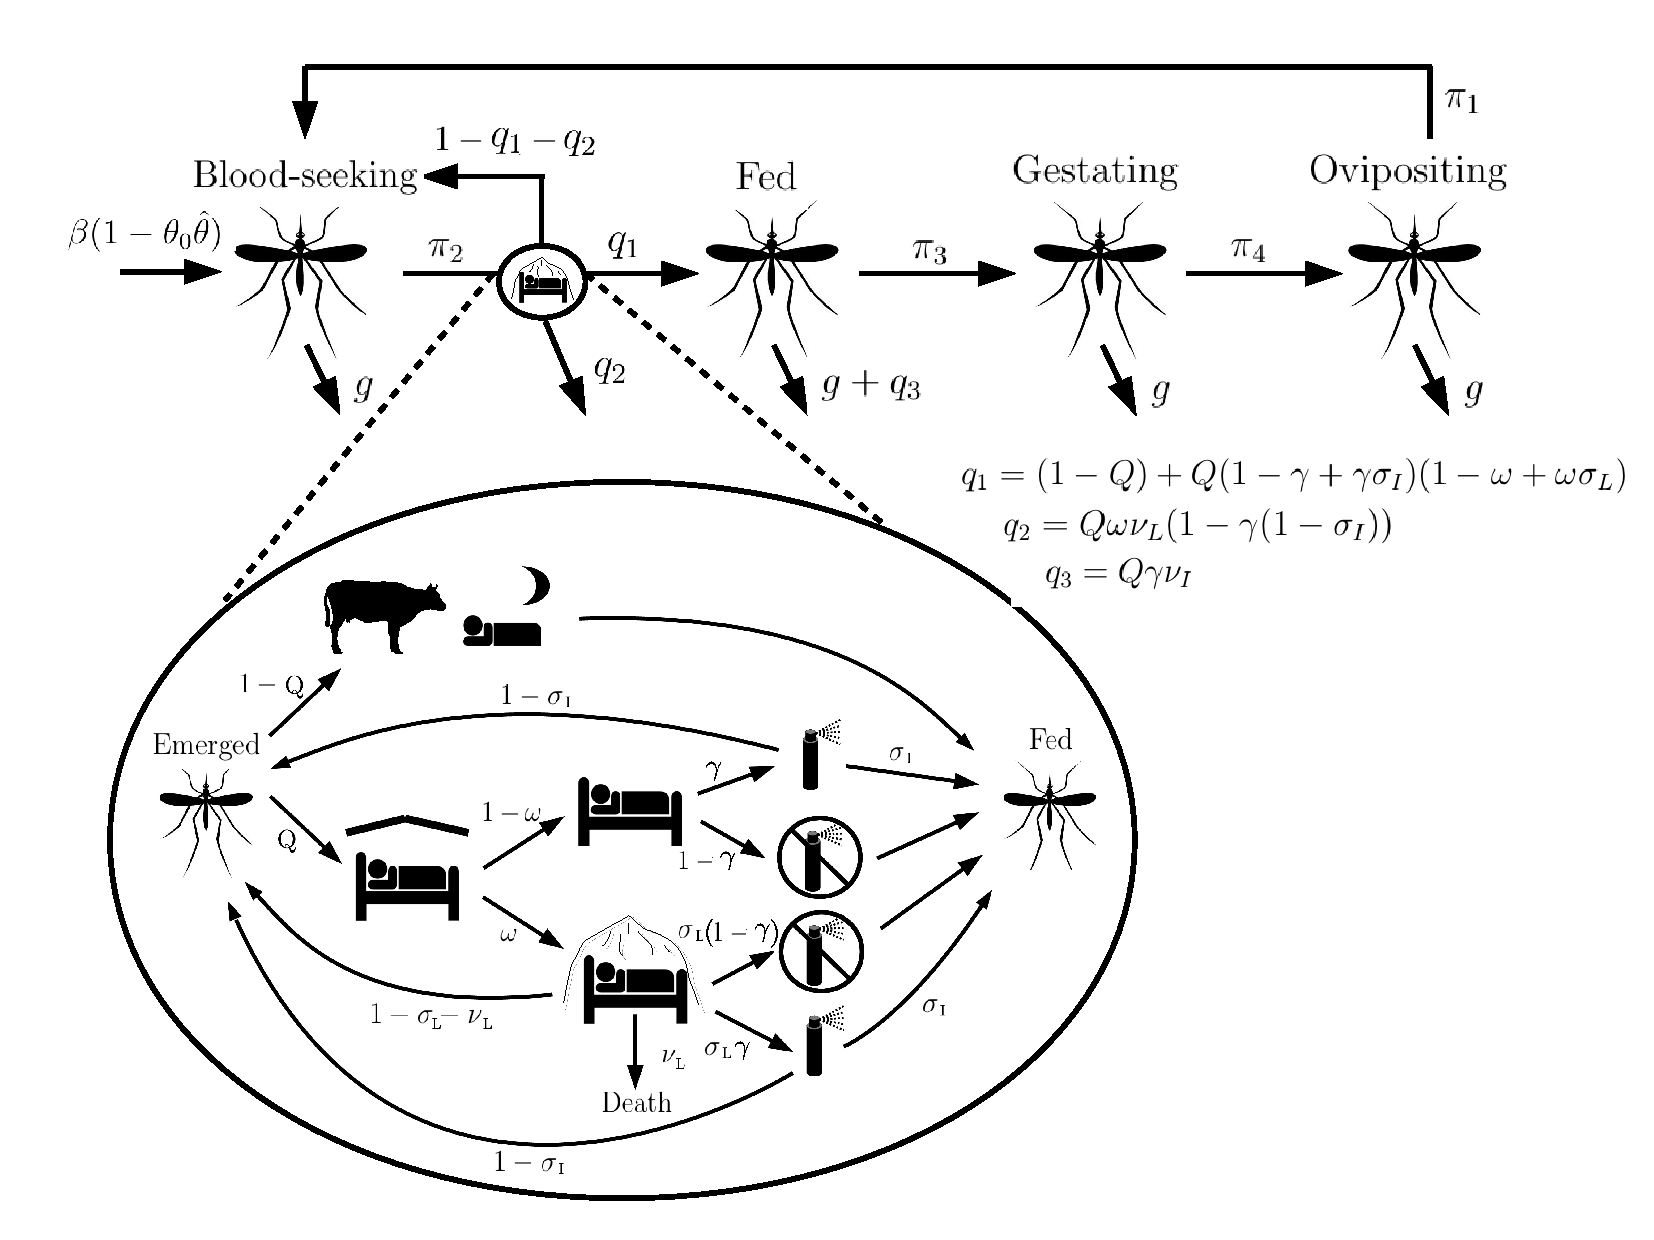
\includegraphics[height=10cm]{Project/Figures/VectorModel/Diagram_VC2019.pdf}
\caption[Gonotrophic cycle model schematic.]{Mosquito feeding dynamics. Outcomes of feeding, death and repeating are all dependant on: proportions of blood meals taken outdoors; vector control coverage; vector control efficacy parameters.}
\label{fig:diag_vec}
\end{center}
\end{figure}

\begin{table*}[t]
\caption[Mosquito parameters and sources.]{Parameters for mosquito biology and vector control (\textit{Anopheles gambiae})}% title of Table
\vspace{.1cm}
\centering % used for centering table
\begin{tabular}{|c|p{54mm}|p{48mm}|c|}% centered columns (4 columns)
\hline                        %inserts double horizontal lines
 & Definition & Value & Source \\ [0.5ex]% inserts table 
%heading
\hline                  % inserts single horizontal line
$Q$ & Fraction of blood-meals indoors & 0.9--0.95 & \cite{Killeen2000} \\
$\pi_2$ & Daily rate of feeding when blood-seeking & 1/0.68 & \cite{Killeen2000} \\
$\delta$ & Mean feeding cycle length (days) & 3 & \cite{Killeen2000} \\
$a$ & Daily rate of feeding on humans & $Q/\delta$ & \cite{Smith2012}  \\
$g$ & Natural daily death rate & 1/14 & \cite{CDCMalaria,le2007} \\
$\sigma_L$ & Probability of feeding in presence of LLINs & 6 holes: 0.121 (0.054--0.188) 80 holes: 0.318 (0.231,0.405) & \cite{Ngufor2011} \\
$\nu_L$ & Probability of pre-meal death in presence of LLINs & 6 holes: 0.495 (0.392--0.597) 80 holes: 0.373 (0.282-0.463) & \cite{Ngufor2011} \\
$\sigma_I$ & Probability of feeding in presence of IRS & 0.894 (0.856--0.931) & \cite{Ngufor2011} \\
$\nu_I$ & Probability of post-meal death in presence of IRS & 0.567 (50.7--62.6) & \cite{Ngufor2011}\\
$\hat{\theta}$ & Proportion of larvae that die from larvicidal treatment & 0.6 (0.5--0.7) & \cite{Kroeger1995}\\
$\beta$ & Adult mosquito emergence rate from larval stages & 1000-100000 (dependent on: disease and setting) & \\
[1ex]      % [1ex] adds vertical space
\hline%inserts single line
\end{tabular}
\label{table:param_vector}% is used to refer this table in the text
\end{table*}

\subsection{Generational distribution}

To gain insight into the age-structure of the vector population we consider a generational formulation of the gonotrophic cycle model, where a subscript $i$ denotes the number of times mosquitoes in a given class have completed the cycle, giving an infinite series of ODEs:
\begin{eqnarray}
\frac{dB_i}{dt} &=& \begin{cases}  \beta(1-\theta) - \pi_2(q_1+q_2)B_{i} -gB_{i} &\mbox{ if } i=0\\ \pi_1O_{i-1} - \pi_2(q_1+q_2)B_{i} -gB_{i} &\mbox{ if } i\geq 1
\end{cases}\\
\frac{dF_i}{dt} &=& \pi_2q_1B_i - \pi_3 F_i - (g+\gamma) F_i \\
\frac{dG_i}{dt} &=& \pi_3F_i - \pi_4G_i - g G_i \\
\frac{dO_i}{dt} &=& \pi_4G_i - \pi_1O_i - g O_i \,.
\label{eqn:dist}
\end{eqnarray}
Adult emergence can only occur into generation $i=0$. Using this model it is possible to calculate the \gls{parity} of the population.

It is reasonable to assume the vector population adjusts essentially instantaneously to equilibrium if vector control in a given setting is fixed, as the vector dynamics are faster than the human dynamics \cite{May1979}. We can hence derive the following relationship between sequential blood-seeking classes:
\begin{equation}
B_n^* = KB_{n-1}^*\,,
\end{equation}
where
\begin{equation}
K = \frac{\pi_1\pi_2\pi_3\pi_4q_1}{(\pi_2(q_1+q_2)+g)(\pi_3+g+q_3)(\pi_4+g)(\pi_1+g)}
\end{equation}
is a constant and $K<1$, this quantity can be interpreted as the gonotrophic cycle survival probability, or the proportion of the vectors that are gravid (have had at least one bloodmeal). As the constant term is less than unity, the difference equation can be solved to get an explicit formula, $B_n^* = K^nB_0^*$, which can be used to calculate the number of vectors in each feeding generation for initial conditions
\begin{equation}
B_0 = \frac{\beta(1-\theta)}{\pi_2(q_1+q_2)+g}\,.
\end{equation}
The proportion of the population that have completed at least one feeding cycle (are parous) is given by
\begin{equation}
1-\frac{B_0}{\sum_i B_i}\,.
\end{equation}

\subsection{Disease dynamics}

The incubation period of LF in the mosquito is approximately 8.5 days \cite{le2007,erickson2009}, and for malaria this can range from 10 to 21 days, depending on parasite species \cite{CDCMalaria}. This means infection cannot be passed on to a new host immediately after the mosquito is infected. Due to the short adult mosquito lifespans (average 10-14 days \cite{le2007}), including the infected but not yet infectious vectors in the force of infection on humans would result in a severe over-estimation when considering the proportion of infectious bites. When modelling the disease dynamics we therefore introduce an exposed class -- where a mosquito has been exposed to infection but is not yet contributing to the net force of infection on the host population. See Tables \ref{table:param_LF} and \ref{table:param_malaria} for full details of the parameter values used and their sources.

\begin{table*}[t]
\caption[LF disease parameters.]{Disease parameters for lymphatic filariasis (\textit{Wuchereria bancrofti})}% title of Table
\vspace{.1cm}
\centering % used for centering table
\begin{tabular}{|c|p{65mm}|p{35mm}|c|}% centered columns (4 columns)
\hline                        %inserts double horizontal lines
 & Definition & Value & Source \\ [0.5ex]% inserts table 
%heading
\hline                  % inserts single horizontal line
$c$ & Proportion bites on infectious humans that result in mosquito infection & 0.37 (0.15--0.6) & \cite{gambhir2008,Subramanian1998}\\
$b$ & Proportion bites from infectious mosquitoes that result in human infection & $1.43\times 10^{-4}$ & Table \ref{tab:Elim} \\
$u$ & Extrinsic incubation period in humans (days) & 285 (192--379)& \cite{Addiss2000} \\
$v$ & Intrinsic incubation period in vector (days) & 8.5 (7--10) & \cite{erickson2009} \\
$1/r$ & Worm fecund life span (years) & 6 & Table \ref{tab:Elim} \\
$x$ & Prevalence of infection in human population & & \\
$\kappa$ & Probability  vector infected after blood meal & $cx$ & \\
[1ex]      % [1ex] adds vertical space
\hline%inserts single line
\end{tabular}
\label{table:param_LF}% is used to refer this table in the text
\end{table*}

\begin{table*}[t]
\caption[Malaria disease parameters.]{Disease parameters for malaria (\textit{Plasmodium falciparum})}% title of Table
\vspace{.1cm}
\centering % used for centering table
\begin{tabular}{|c|p{74mm}|p{32mm}|c|}% centered columns (4 columns)
\hline                        %inserts double horizontal lines
 & Definition & Value & Source \\ [0.5ex]% inserts table 
%heading
\hline                  % inserts single horizontal line
$c$ & Proportion bites on infectious humans that result in mosquito infection & 0.55 (0.47-0.63) & \cite{Smith2010} \\
$b$ & Proportion bites from infectious mosquitoes that result in human infection & 0.037 (0.018-0.055) & \cite{Killeen2000} \\
$u$ & Intrinsic incubation period in humans (days) & 12 (8-23) & \cite{Boyd1937} \\
$v$ & Extrinsic incubation period in vector (days) & 10 (10-21) & \cite{Gary2001}\\
$1/r$ & Mean human infection duration (days) & 14 & \cite{CDCMalaria} \\
$x$ & Prevalence of infection in human population & varied & \\
$\kappa$ & Probability  vector infected after blood meal & $cx$ & \\
[1ex]      % [1ex] adds vertical space
\hline%inserts single line
\end{tabular}
\label{table:param_malaria}% is used to refer this table in the text
\end{table*}

We consider three disease states: susceptible ($S$), exposed ($Y$) and infectious ($Z$). Extending the ODE model (as in Eqn \ref{eqn:ODE}) to include disease requires sub-dividing each stage of the cycle into these three states, giving a new system of twelve ODEs. We assume adult emergence only occurs in the susceptible vector population. Assuming a prevalence $x$ in the human population and a probability $c$ that a vector becomes infected after biting an infectious human, then a proportion $xc$ of susceptible vectors moving from blood-seeking to fed become exposed to disease; all exposed mosquitoes can become infected, this occurs at rate $1/v$ where $v$ is the average vector incubation period. Due to timescales of infection and vector lifespan we do not consider recovery from infection. See Fig. \ref{fig:diag_vec_SEI} for a diagram of the full model dynamics.

\begin{figure}[ht]
\begin{center}
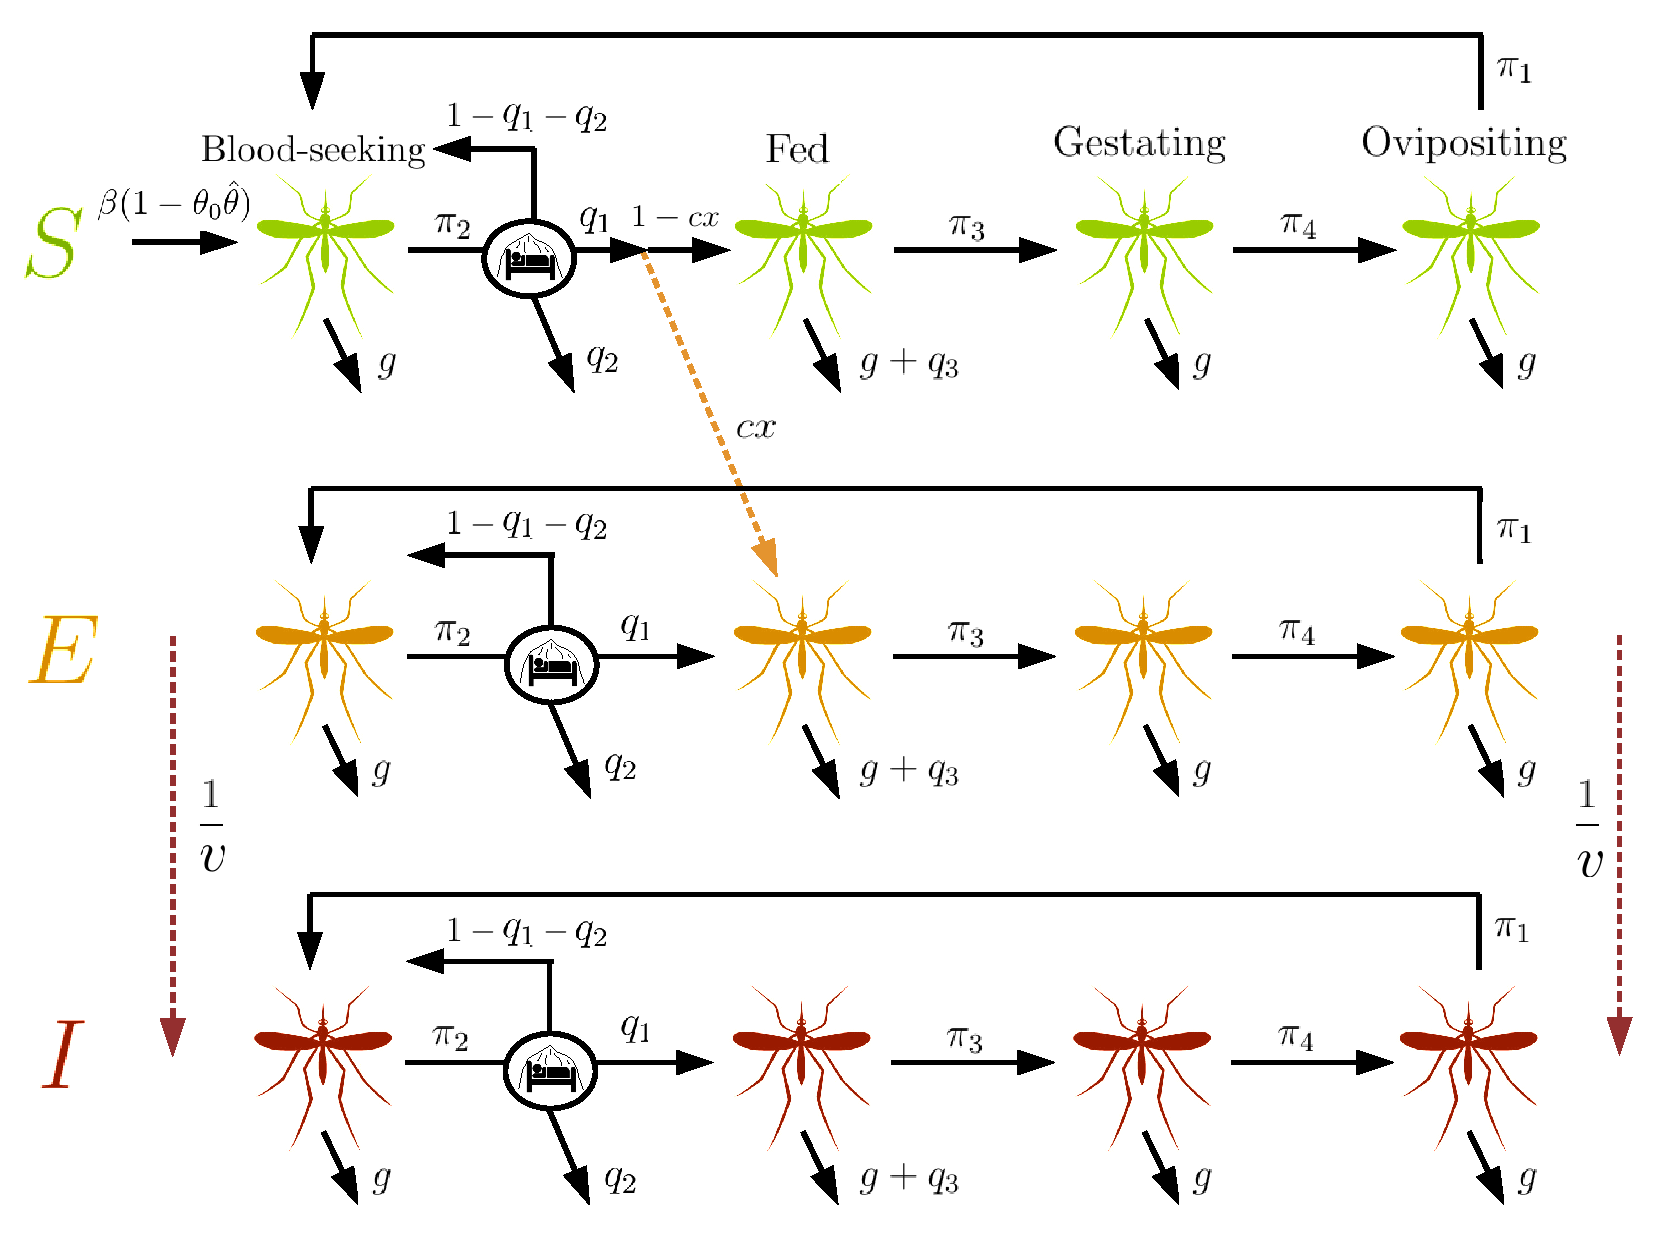
\includegraphics[height=9cm]{Project/Figures/VectorModel/Diagram_SEI2019.pdf}
\caption[Mosquito disease model schematic.]{Mosquito disease dynamics. Birth occurs in the susceptible (S) state, then during the feeding process vectors can become exposed with probability $\hat{p}=xc$ given a successful feed. Exposed (Y) vectors from all stages become infectious (Z) at rate $1/v$, where $v$ is the incubation period. Straight lines indicate transitions, diagonal lines represent deaths and dashed lines are infection events.}
\label{fig:diag_vec_SEI}
\end{center}
\end{figure}

\subsubsection{Generational distribution with disease}

%Considering instead the generational distribution model (Eqn. \ref{eqn:dist}) we can use the binomial probability, $p$, of a successful feed leading to a new vector infection to calculate the probability a mosquito is infected by the end of generation $k$:
%\begin{equation}
%p^{(k)} = \sum_{j=0}^k (1-p)^jp\,.
%\label{eqn:p}
%\end{equation}

%Assuming the vector incubation period is equivalent to approximately $n$ generations, we can calculate the equilibrium number of exposed and infected mosquitoes:
%\begin{eqnarray}
%\mbox{\# Exposed} = \sum_{i=1} E_i^* p^{(i-1)}\,,\\
%\mbox{\# Infected} = \sum_{i=n} E_i^* p^{(i-n)}\,.
%\label{eqn:numinf}
%\end{eqnarray}
%These values can be normalised to give prevalence of exposure and infection in the vector population.

%The probability of a vector in the emerged class surviving until it has successfully fed is given by
%\begin{equation}
%\mathbb{P}[\mbox{Successfully feed}] = \frac{\pi_2p_1}{\pi_2(p_1+p_2)+\delta}\,,
%\end{equation}
%which can then be used to consider the proportion of exposed mosquitoes that successfully bite and hence could go on to transmit infection. In the absence of bednets this probability is $0.980$, but increasing bednet coverage to $40\%$ results in a decrease to $0.841$, reflecting a reduction in the chance of a vector passing on infection in addition to the reduction in vector prevalence. %reword this? use better statistics - consider incubation period!

Consider instead the generational distribution model at equilibrium (Eqn. \ref{eqn:dist}), such that the number of blood-seeking vectors in generation $n$ is $K^nB_0$. It is sufficient to consider the blood-seeking class as this is the stage of the feeding cycle where vectors have potential to pick up or transmit disease through biting. If we define the binomial probability, $\hat{p}=xc$, of a successful feed leading to a new vector infection, then the probability a mosquito becomes exposed during generation $n$ is $\hat{p}^{(n)}=(1-\hat{p})^{n-1}\hat{p}$. Hence the probability a mosquito has been exposed before generation $n$ is $[1-(1-\hat{p})^n]$. Combining these gives the number of vectors in generation $n$ that are already infected:
\begin{equation}
B_0K^n[1-(1-\hat{p})^n]\,.
%C^nE_0^*(1-p)^{n-1}p\,.
\label{eqn:probinfect}
\end{equation}
The total number of diseased (exposed or infectious) vectors is given by summation across the generations;
\begin{eqnarray}
D &=& B_0\sum_{n=0}^{\infty} [K^n - K^n(1-\hat{p})^n]\\
&=& \frac{\hat{p}KB_0}{(1-K)(1-K+\hat{p}K)}\,.
%%N_D &=& \sum_{n=1}^{\infty}(1-p)^{n-1}pC^nE_0^*\\
%%&=& pE_0^*C\sum_{n=0}^{\infty}(1-p)^nC^n\\
%%&=& \frac{pE_0C}{1-C(1-p)}\,.
\end{eqnarray}

If the incubation period is assumed to be equivalent to $N$ generations (or cycles), then the probability of surviving until infectious is given by $K^N$ and can be treated as a multiplicative factor when calculating the numbers of infectious and exposed vectors:

\begin{eqnarray}
Z &=& K^ND\,,\\
Y &=& D - Z\,.
\end{eqnarray}
%If incubation period is assumed to be equivalent to $M$ generations then the probability a vector will survive at least $M$ cycles, which is given by
%\begin{equation}
%\sum_{j=M}^{\infty}C^j\,,
%\end{equation}
%can be used to calculate the number of infectious vectors:
%\begin{eqnarray}
%N_I &=& \sum_{n=1}^{\infty}\bigg(\sum_{j=M}^{\infty}C^j\bigg)p^{(n)}C^nE_0^*\\
%&=& \sum_{n=1}^{\infty}\bigg(\sum_{j=M}^{\infty}C^{j}\bigg)\bigg((1-p)^{n-1}p\bigg)\bigg(C^nE_0^*\bigg)\\
%&=& pE_0^*C\bigg(\sum_{j=0}^{\infty}C^{j+M}\bigg)\bigg(\sum_{n=1}^{\infty}(1-p)^{n-1}C^{n-1}\bigg)\\
%&=& pE_0^*C^{M+1}\bigg(\frac{1}{1-C}\bigg)\bigg(\frac{1}{1-C(1-p)}\bigg)\\
%&=&\frac{pE_0^*C^{M+1}}{(1-C)(1-C(1-p))} \,.
%\end{eqnarray}
These values can be normalised to give prevalence of exposure and infection in the vector population. Here we are fixing the range of possible EIP values in relation to the cycle length, with EIP $\in (N-1,N]$ gonotrophic cycles. This simplifies the system and allows us to derive analytical forms of the quasi-equilibrium solution of the model and a number of key transmission statistics. This assumption is not unreasonable given the comparatively narrow range of values quoted in the literature \cite{erickson2009}.

The force of infection on humans, $FoI_H$, is proportional to the number of infectious mosquitoes and the vector bite rate:
\begin{equation}
FoI_H \propto \pi_2q_1Z\,.
\end{equation}

\subsection{Transmission measures}
\label{sec:EpiMeasures}

There are a number of statistics commonly used to described transmission of vector-borne diseases. In the field, human landing catches are often used to estimate the \gls{EIR} (\acrshort{eir}), the expected number of infectious bites received by a single host each year \cite{Kilama2014}. A second measure, vectorial capacity, denotes the total number of infectious bites that would eventually arise from all the mosquitoes that bite a single infectious human on a single day \cite{Smith2010}. From the vectorial capacity we can derive the basic reproductive number, $R_0$, for vector borne diseases. This differs from the usual interpretation of $R_0$ for non-vector diseases by focusing on the vector dynamics and is also occasionally interpreted as $R_0^2$, describing the number of new infectious mosquitoes that would arise from a single infectious mosquito after one parasite generation \cite{Smith2010}. These three key measures are given by the following formulas:

\noindent Entomological innoculation rate (EIR):

\begin{equation}
E = maz \,,
\end{equation}

where $m$ is the ratio of mosquitoes to humans, $a$ is the blood feeding rate on humans, and $z$ is the fractional prevalence of infectious vectors.

\noindent Vectorial capacity:

\begin{equation}
V = \frac{ma^2p^v}{-\ln(p)} = \frac{ma^2}{g}e^{-gv} \,,
\end{equation}

where $p$ is the vector daily survival probability and $v$ is the extrinsic incubation period in the vector. Alternatively, $g$ is the instantaneous vector death rate.

\noindent Basic reproductive number:

\begin{equation}
R_0 = \frac{ma^2bc}{gr}e^{-gv} = \frac{ma^2bc}{-\ln(p)r}p^v = \frac{Vbc}{r} \,,
\end{equation}

where $b$ is the probability a bite from an infectious vector infects a human, $c$ is the probability a bite on an infectious human infects a vector, and $r$ is the human disease recovery rate.

\noindent We can calculate the total number of diseased vectors (exposed plus infectious), $D$, dependent on vector control parameters and coverage:

\begin{eqnarray}
D := Y+Z = \frac{\kappa KE_0}{(1-K)(1-K+\kappa K) \,, }\\
E_0 = \frac{\beta(1-\theta)}{\pi_2(q_1+q_2)+g} \,.
\end{eqnarray}

$E_0$ is the number of exposed vectors and $\kappa = cx$ is the probability one human blood feed results in a vector infection ($x$ is the prevalence of disease in the human population).

\noindent From this we can get the total number of infectious vectors:

\begin{equation}
Z = K^ND\,,
\end{equation}

and hence directly calculate our useful statistics. For example, the EIR is given by:

\begin{equation}
E = maK^N\bigg(\frac{\kappa KE_0}{(1-K)(1-K+\kappa K)}\bigg)\frac{1}{M}
\end{equation}

In the absence of interventions the mean feeding cycle length is,

\begin{equation}
\delta = 1/\pi_1+1/\pi_2+1/\pi_3+1/\pi_4\,,
\end{equation}

where $1/\pi_2$ is the average time to hunt and take a blood meal. IRS and larvicides won't impact hunting time, but the repelling effect of bednets will result in some vectors taking longer to move from emerged to fed.

If we assume a repelled vector begins the hunting process from scratch, then the expected time taken to successfully feed will be equal to the time taken to feed given a successful first attempt plus the expected time taken to feed scaled by the proportion of vector that repeat on any given attempt.

\begin{eqnarray}
\mathbb{E}[\mbox{Time to feed}] &=& \mathbb{E}[\mbox{Time }|\mbox{ Successful attempt}] \\
&& + \mathbb{P}[\mbox{Repeat}]\mathbb{E}[\mbox{Time to feed}]\\
\mathbb{E}[\mbox{Time to feed}] &=& \frac{1}{\pi_2} + Q\omega(1-\sigma-\nu)\mathbb{E}[\mbox{Time to feed}]\\
\mathbb{E}[\mbox{Time to feed}] &=& \frac{1}{\pi_2(1-Q\omega(1-\sigma-\nu))}
\end{eqnarray}

Now we can express overall feeding cycle length, $\delta$, in terms of bednet parameters:

\begin{eqnarray}
\delta &=& \frac{1}{\pi_2(1-Q\omega(1-\sigma-\nu))} + \frac{1}{\pi_3}+\frac{1}{\pi_4}+\frac{1}{\pi_1}\\
&=& \frac{(\pi_1\pi_3+\pi_1\pi_4+\pi_3\pi_4)\pi_2(1-Q\omega(1-\sigma-\nu))+\pi_1\pi_3\pi_4}{\pi_1\pi_2\pi_3\pi_4(1-Q\omega(1-\sigma-\nu))}
\end{eqnarray}

and the human blood feeding rate is given by:

\begin{eqnarray}
a &=& Q\bigg(\frac{1}{\pi_2(1-Q\omega(1-\sigma-\nu))} + \frac{1}{\pi_3}+\frac{1}{\pi_4}+\frac{1}{\pi_1}\bigg)^{-1}\\
&=& Q\frac{\pi_1\pi_2\pi_3\pi_4(1-Q\omega(1-\sigma-\nu))}{(\pi_1\pi_3+\pi_1\pi_4+\pi_3\pi_4)\pi_2(1-Q\omega(1-\sigma-\nu))+\pi_1\pi_3\pi_4}
\end{eqnarray}

The ratio of vectors to humans $m$, can be scaled by changes in the mosquito population ($m=M/H$), where

\begin{equation}
M = \sum_{i=0}^{\infty}E_0K^i = \frac{E_0}{1-K}
\end{equation}

and $K$ describes the probability of surviving each feeding cycle, with dependence on vector control parameters included in $E_0$ and $K$.

The death rate will depend on IRS and bednet usage. We can relate the probability of a vector surviving one feeding cycle, $K$, to a per cycle death rate $-ln(K)$, then we have

\begin{equation}
g = \frac{-ln(K)}{\delta}
\end{equation}

as the instanenous daily death rate.

Now that we have vector control dependent expressions for all relevant parameters, these can be substituted into our equations to calculate key transmission measures, such as $R_0$. In the presence of vector control measures, we relabel $R_0$ as the effective reproductive number under control, $R_e$.


%The probability of a vector in the emerged class surviving until it has successfully fed is given by
%\begin{equation}
%\mathbb{P}[\mbox{Successfully feed}] = \frac{\pi_2p_1}{\pi_2(p_1+p_2)+\delta}\,,
%\end{equation}
%which can then be used to consider the proportion of exposed mosquitoes that successfully bite and hence could go on to transmit infection. In the absence of bednets this probability is $0.980$, but increasing bednet coverage to $40\%$ results in a decrease to $0.841$, reflecting a reduction in the chance of a vector passing on infection in addition to the reduction in vector prevalence. %reword this? use better statistics - consider incubation period!
\FloatBarrier 

\subsection{Host dynamics}
\label{sec:Host}

Using the formulation laid out in the EPIFIL model \cite{Norman2000_epifil}, whilst simplifying to neglect acquired immunity and age dependency in humans, it is possible to write down an ODE model for LF host infections. Disease magnitude is described in terms of the mean worm burden ($W$) and mean mf count per 20$\mu$l of blood ($M$); acquisition of disease is dependent on the force of infection of the vector on the host population, $F_{V\rightarrow H}$, taken to be the prevalence of disease in the vector population.
\begin{eqnarray}
\frac{dW}{dt} &=& \lambda\frac{V}{H}\psi_1\psi_2\psi_3F_{V\rightarrow H} - \mu W\\
\frac{dM}{dt} &=& \alpha W - \gamma M \,.
\end{eqnarray}

Infection is described using the rate at which humans are bitten, which is given as the number of bites per mosquito per unit time, $\lambda$, multiplied by the ratio of vectors to hosts. This is combined with the proportion of L3 leaving the mosquito per bite ($\psi_1$), the proportion of these that enter the host ($\psi_2$), the proportion of L3 in the host that then develop into adult worms, and the force of infection ($F_{V\rightarrow H}$); death of adult worms occurs at rate $\mu$. Adult worms produce mf at rate $\alpha$ per 20$\mu$l of blood and mf die at rate $\gamma$.

\begin{table*}[t]
\caption[Host transmission model parameters.]{Parameter definitions and values for host model, all taken from Norman et al (2000) \cite{Norman2000_epifil}.}% title of Table
\vspace{.1cm}
\centering % used for centering table
\begin{tabular}{c l c}% centered columns (4 columns)
\hline\hline                        %inserts double horizontal lines
Parameter & Definition & Value (per month) \\ [0.5ex]% inserts table 
%heading
\hline                  % inserts single horizontal line
$\lambda$ & Number of bites per mosquito & 10 \\% inserting body of the table
$\alpha$ & Production rate of mf per worm & 2  \\
$k(M)$ & Aggregation parameter & $0.0029+0.0236\times M$ \\[1ex]      % [1ex] adds vertical space
\hline%inserts single line
\end{tabular}
\label{table:param_host}% is used to refer this table in the text
\end{table*}

Host prevalence, $P$, can then be estimated by considering the probability of an individual having greater than zero parasites per 20$\mu$l of blood:
\begin{equation}
P(M) = 1 - (1+M/k)^{-k}\,.
\label{eqn:prev}
\end{equation}

The vector model equilibrium depends on the probability one successful blood feed results in a mosquito becoming infected. Since vector dynamics are much faster than host dynamics we assume that they instantaneously adjust to quasi-equilibrium, hence we can use the current state of host infection to calculate the new vector equilibrium at each step of evaluating the host model and determine the force of infection on the host population at that point in time.

The model is hence evaluated in the following way:
\begin{enumerate}
\item The rate at which humans are bitten is fitted to the required equilibrium host prevalence in the absence of vector control, using the relationship between $M$ and prevalence given in Equation \ref{eqn:prev}.
\item The type and coverage of vector control is chosen.
\item At each step equilibrium vector prevalence is re-evaluated based on the host prevalence. 
\item The values of $W$ and $M$ are recorded at each time step; host prevalence can then be estimated if required.
\end{enumerate}

\section{Results}

In all of the following results, unless otherwise specified, we assume a 40\% human prevalence (infectious disease) to reflect a high-endemicity setting. Results for LF parameters are presented first, followed by results for malaria parameters. 

First we investigate the age-structure properties of the mosquito model and what this can tell us about transmission. We consider the age of a mosquito in terms of the number of generations, or gonotrophic cycles, it has lived through. Figure \ref{fig:propEI} shows the age-dependent probability of a vector being exposed ($E$) or infectious ($I$) by the number of gonotrophic cycles completed, in the absence of vector control. There is zero probability of being exposed or infectious in the newly emerged generation, and mosquitoes then have a probability of becoming exposed each time they feed, according to Eqn \ref{eqn:probinfect}. For LF this probability is taken to be $0.37$ if the bloodmeal is taken on an infectious host and it is assumed that it takes 3 feeding cycles to reach infectivity. For malaria these parameter are $0.4$ and 4 feeding cycles respectively, so vectors can't be infectious until they have completed their 4th feeding cycle, this means the ratio of infectious to exposed vectors is lower, with fewer infectious vectors overall. 

\begin{figure}[ht]
\begin{center}$
\begin{array}{cc}
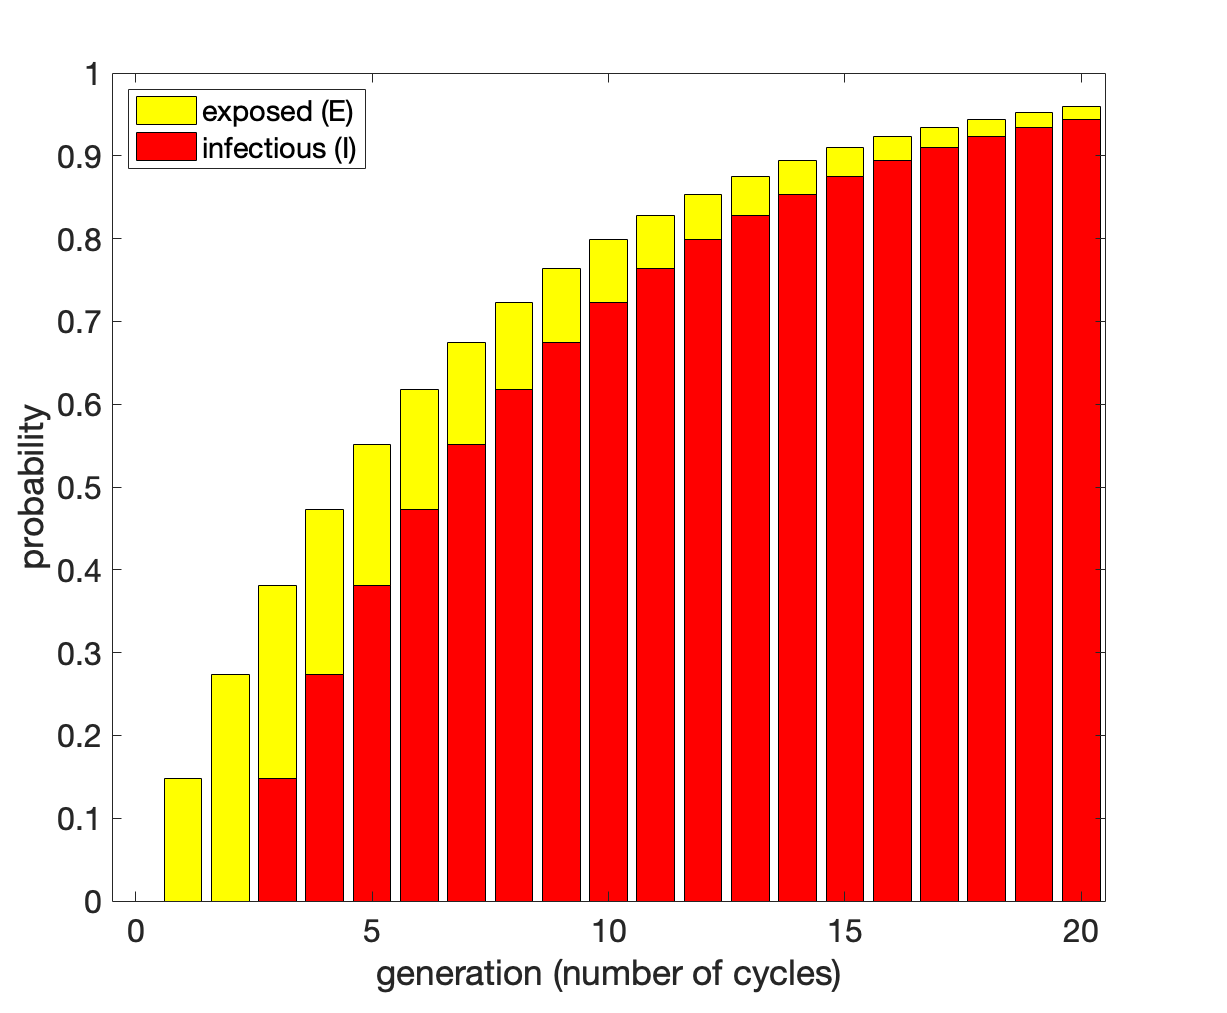
\includegraphics[height=5.8cm]{Project/Figures/VectorModel/LF/populationpropEI.png}&
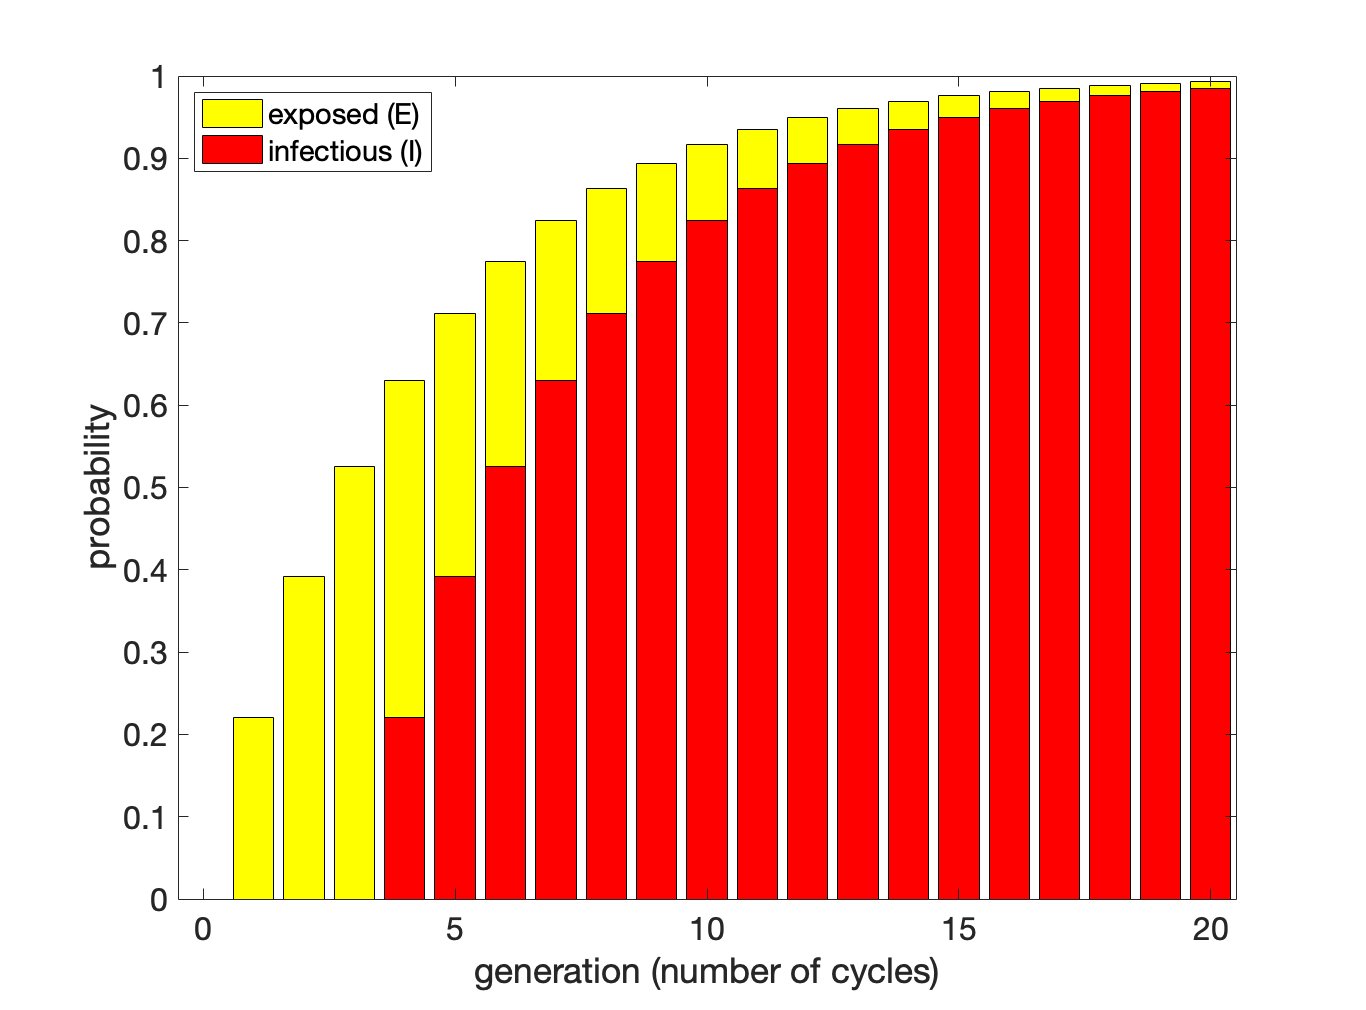
\includegraphics[height=5.8cm]{Project/Figures/VectorModel/Malaria/populationpropEI.png}
\end{array}$
\caption[Probability of exposure and infection (vector).]{Stacked bar plots showing the probability of a vector being exposed (yellow) or infectious (red) for each cycle generation. Left: For LF at 40\% host mf prevalence. Right: For malaria at 40\% host prevalence.}
\label{fig:propEI}
\end{center}
\end{figure}

\subsection{Lymphatic filariasis}

Figures \ref{fig:8controls_LF} and \ref{fig:4controls} show how the generational distribution of the mosquito population, and the presence of infection, varies according to the three different vector control interventions. We can clearly see the difference in the effects between the larvicides, which just impact the vector population size, and the other interventions, which also repel living vectors and reduce feeding. 

\begin{sidewaysfigure}[p] 
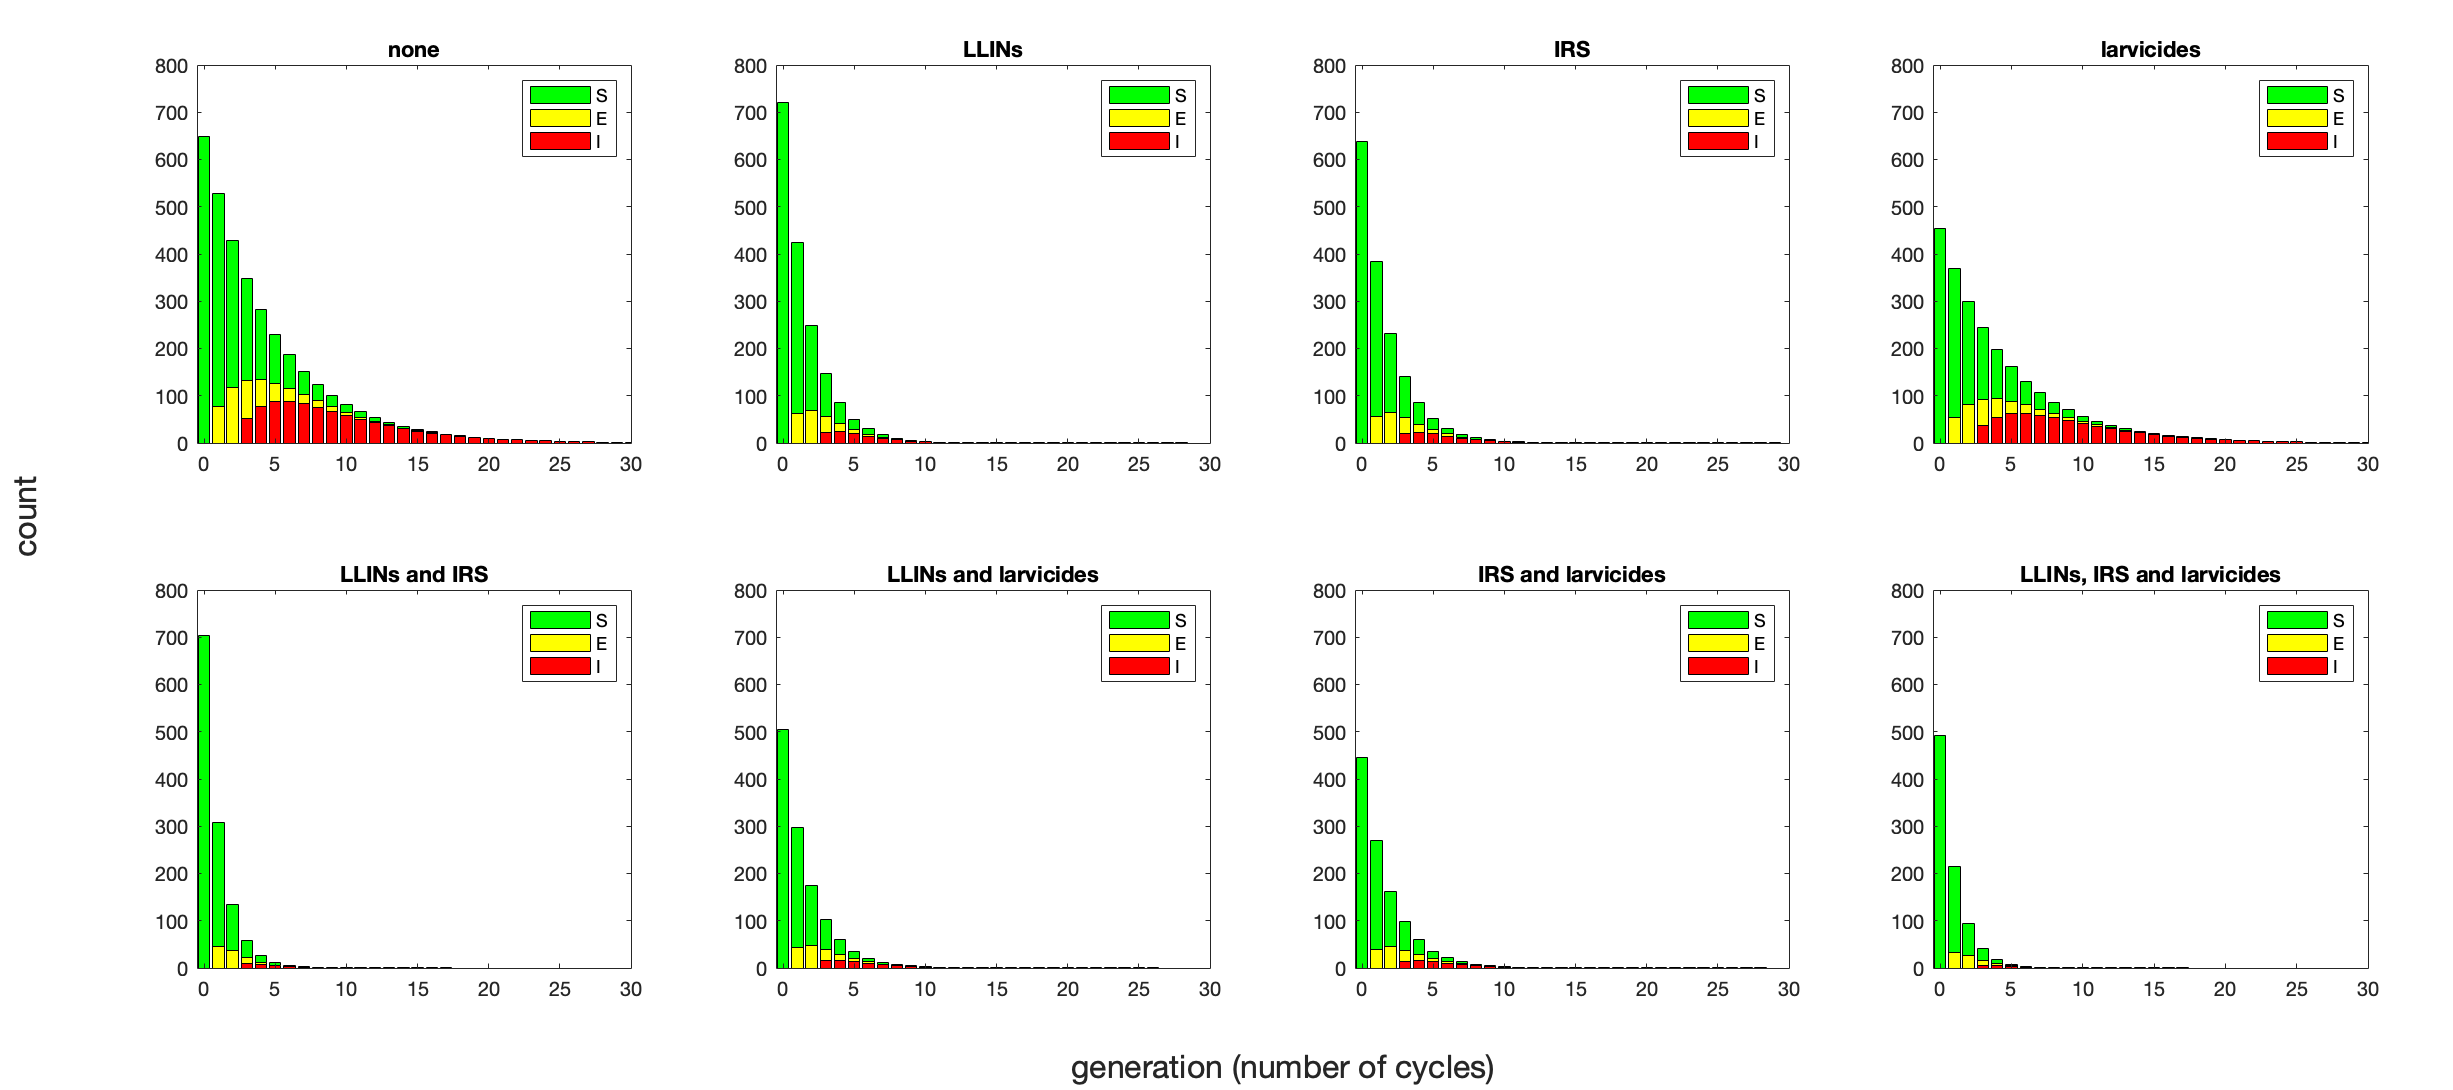
\includegraphics[height=9.7cm]{Project/Figures/VectorModel/LF/populationhist_8controls.png}
\caption[Age distribution with infection (vector count).]{Bar plots showing the age distribution of a vector population at equilibrium (total count, indexed by number of gonotrophic cycles completed) with a variety of combinations of vector control interventions. All interventions are assumed to have 50\% coverage. Bars are coloured by the proportion of vectors in each cycle generation that are susceptible (green), exposed (yellow) and infectious (red) for LF at 40\% host mf prevalence. Malaria results are presented in Figure \ref{fig:8controls_Ma}.}
\label{fig:8controls_LF}
\end{sidewaysfigure} 

LLINs, which have the highest repelling rate, cause a relative increase in the number of \gls{nulliparous} vectors (those who have taken no bloodmeals), as well as an increased death rate due to contact with insecticides. This leads to many fewer vectors in the older generations, in which infectious disease is the most prevalent and a higher frequency of mosquitoes in the younger generations, in particular generation $0$. IRS acts in a similar way, but repelling is less common and the killing effect is stronger. 

\begin{figure}[ht]
\begin{center}
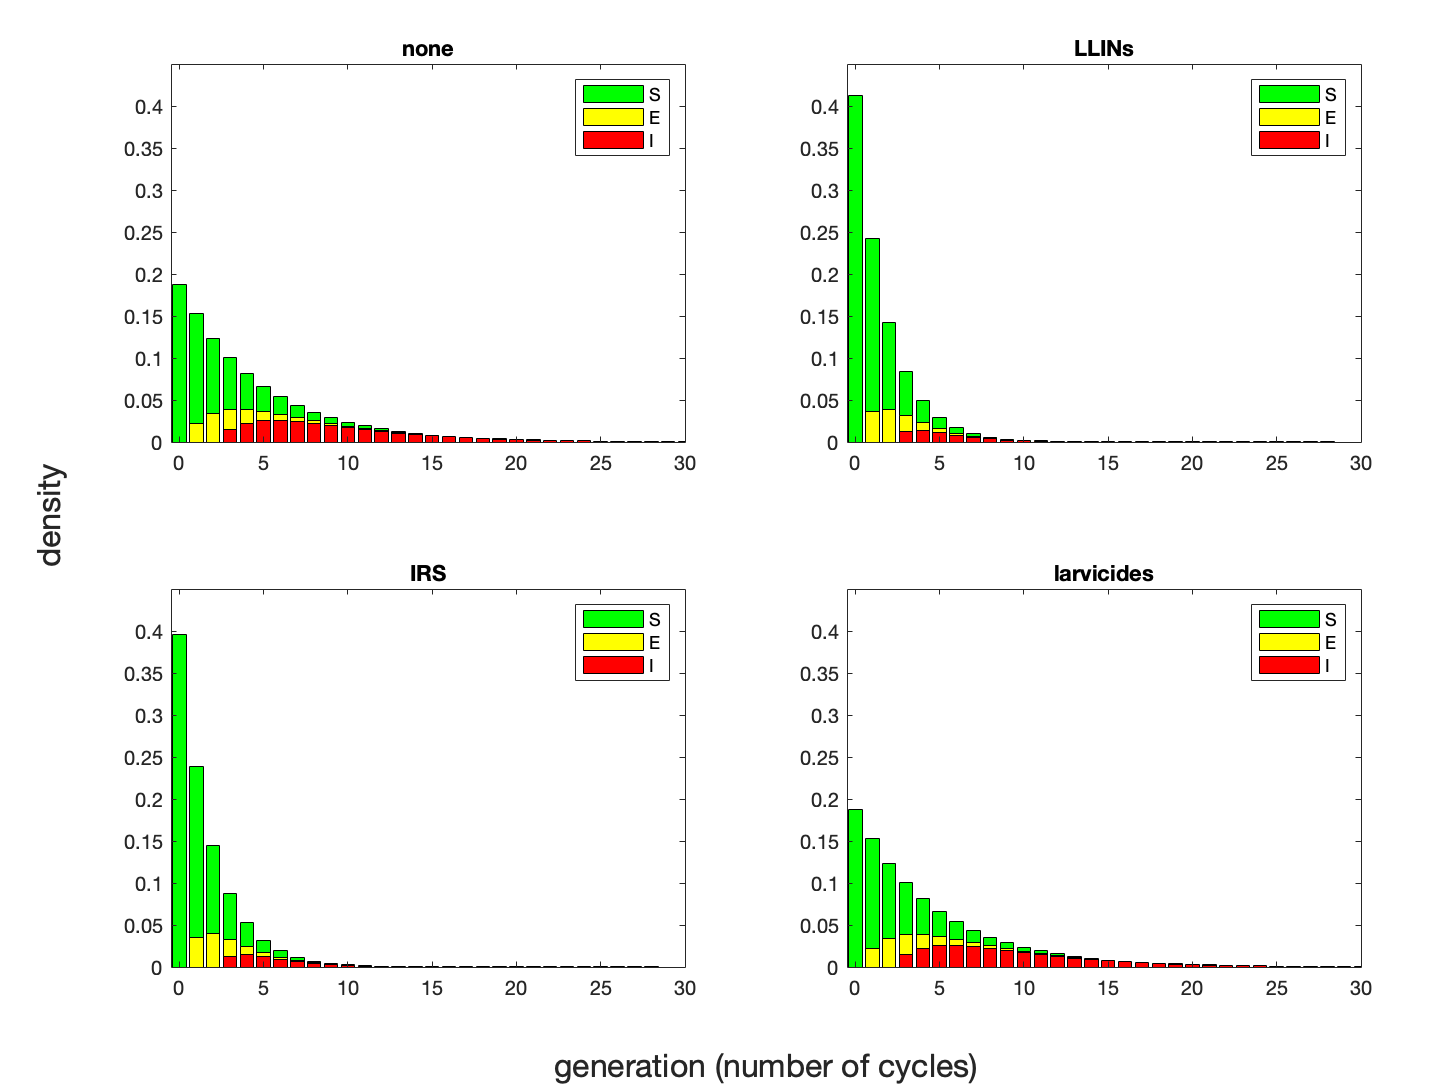
\includegraphics[height=11cm]{Project/Figures/VectorModel/LF/populationhist_4controls_density.png}
\caption[Age distribution with infection (vector density).]{Histograms showing the age distribution of a vector population (density, indexed by number of gonotrophic cycles completed) for single vector control interventions. All interventions are assumed to have 50\% coverage. Bars are coloured by the proportion of vectors in each cycle generation that are susceptible (green), exposed (yellow) and infectious (red) for LF at 40\% host mf prevalence.}
\label{fig:4controls}
\end{center}
\end{figure}

Larvicides act by reducing the emergence rate, and hence the overall population size, but as this doesn't impact adult feeding or death rates the age distribution of the population remains proportionally the same, meaning there is still a substantial infectious subset of older vectors. This is easily seen in Figure \ref{fig:4controls}, which shows the proportional distribution rather than the raw count of vectors; the larvicide histogram is an exact replica of the histogram representing no vector control measures. The LLIN and IRS histograms show more than twice the proportion of null parous vectors (around 40\% as opposed to under 20\%).

The control combinations (bottom row Figure \ref{fig:8controls_LF}) give the best outcome when adult-based control measures are combined - either IRS and LLINs or all three controls. Combining larvicides with either IRS or LLINs simply gives a scaling of the single repeating intervention effect. As the number of infectious vectors is already very low in the case of just IRS or LLIN usage, this scaling is unlikely to have an impact on transmission viability that is reflective of the level of programmatic effort required to find and treat 50\% of larval sites.

\begin{sidewaysfigure}[p] 
\begin{center}$
\begin{array}{cc}
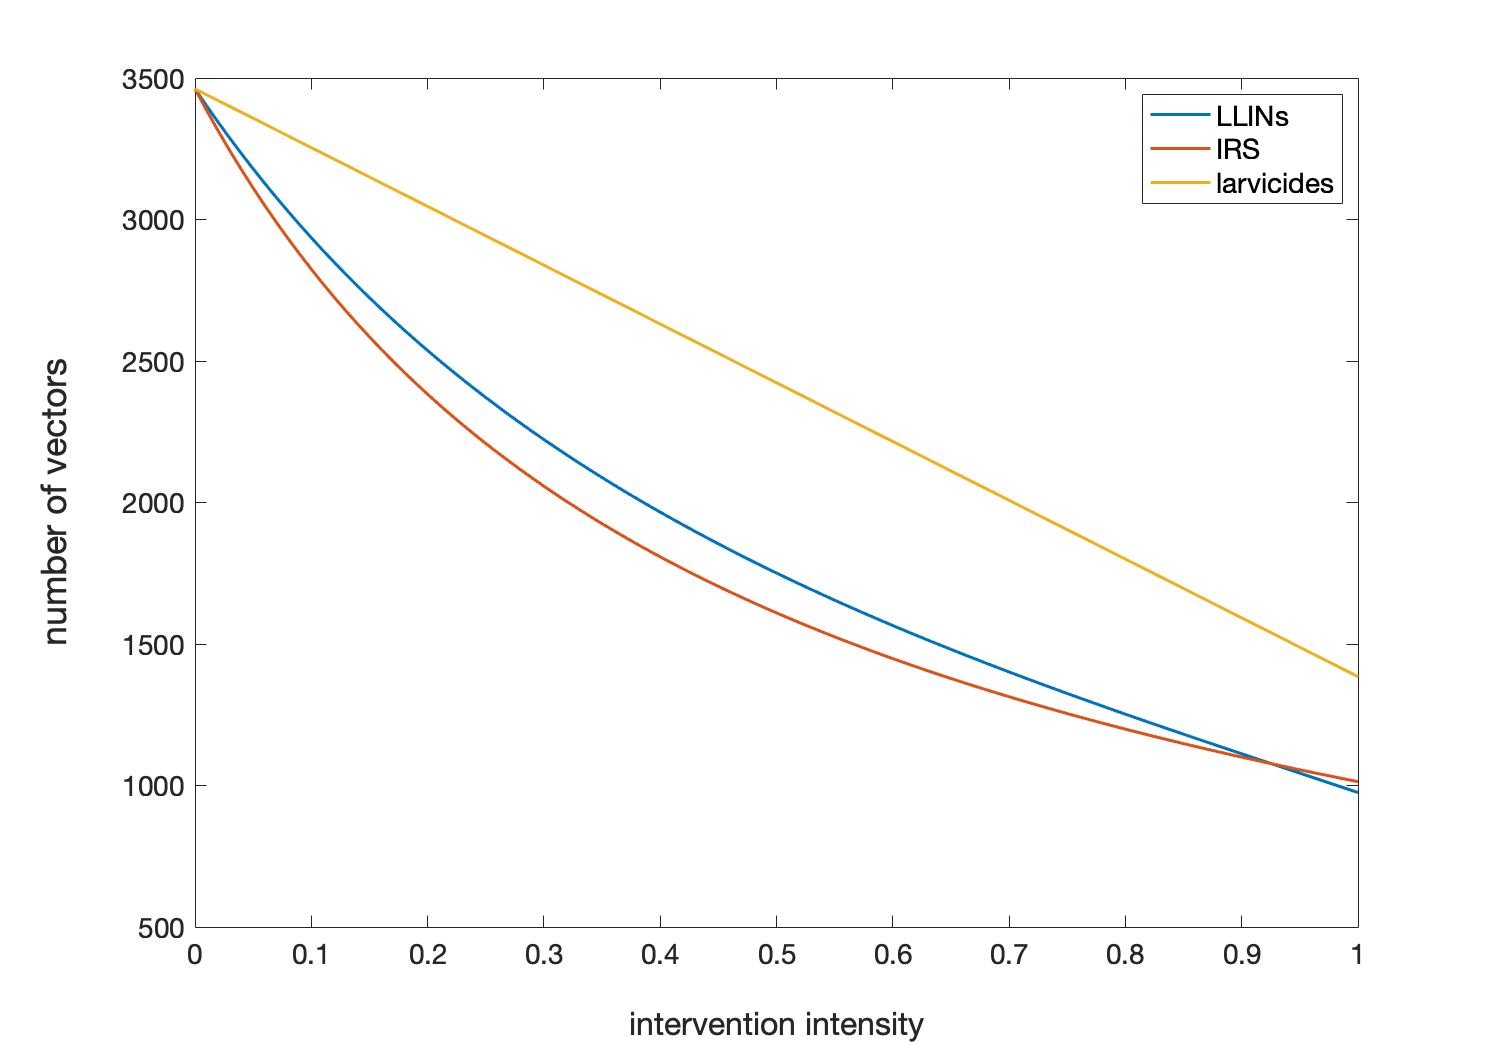
\includegraphics[height=6.7cm]{Project/Figures/VectorModel/LF/NumVec.png} & 
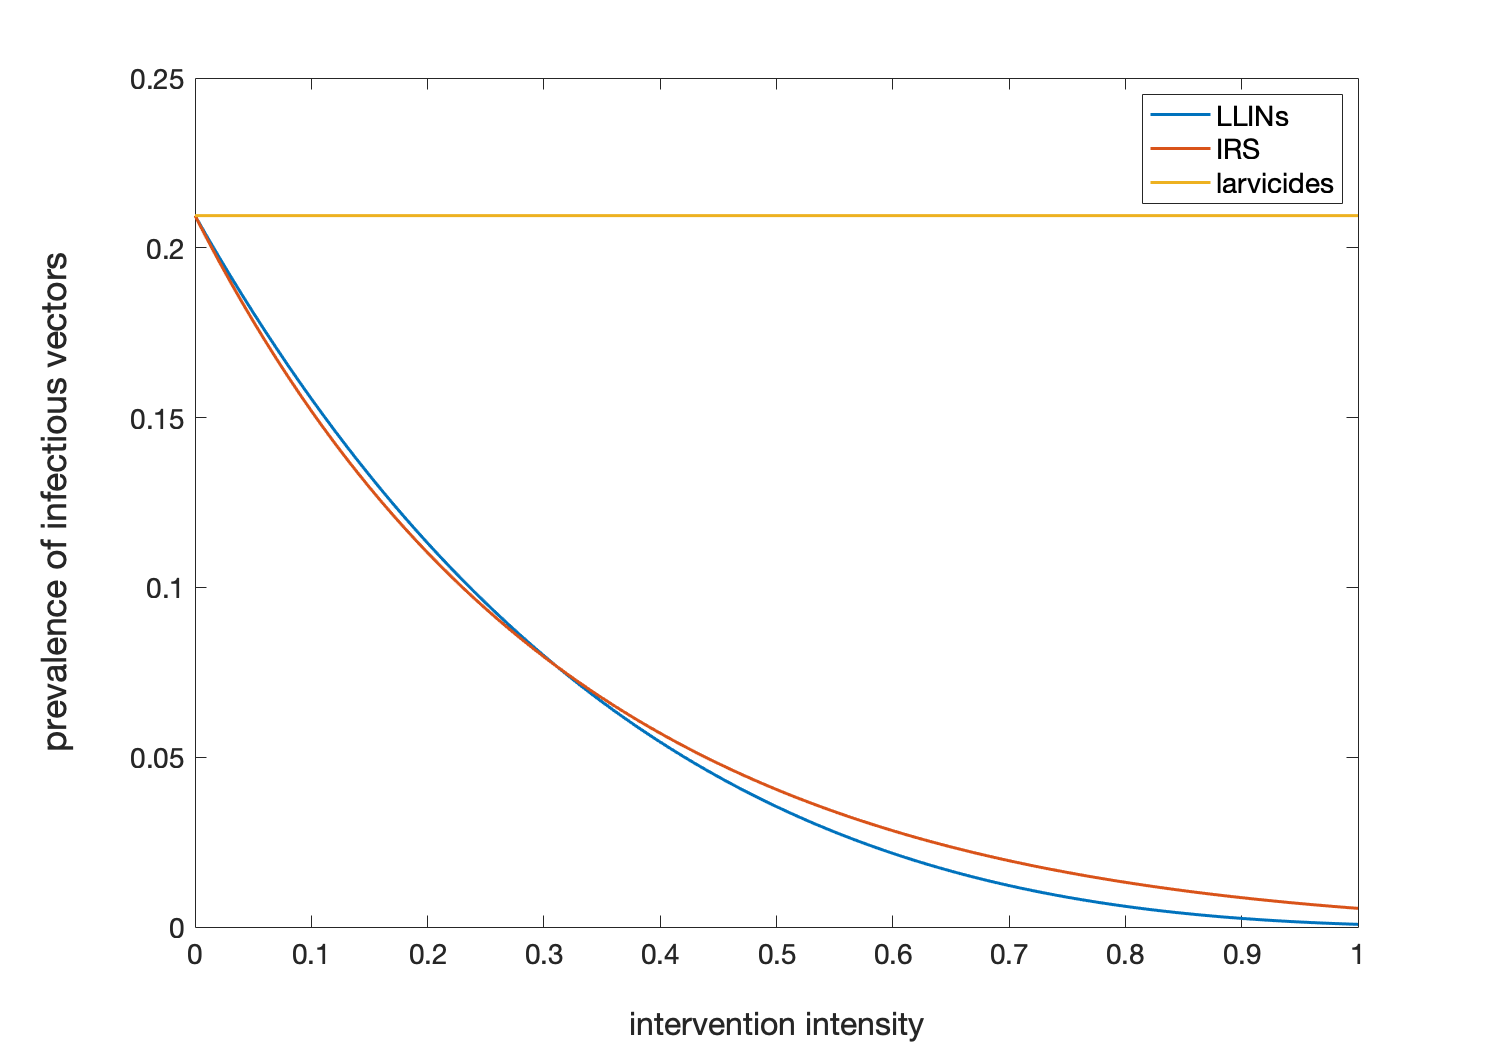
\includegraphics[height=6.7cm]{Project/Figures/VectorModel/LF/VecPrev.png} \\
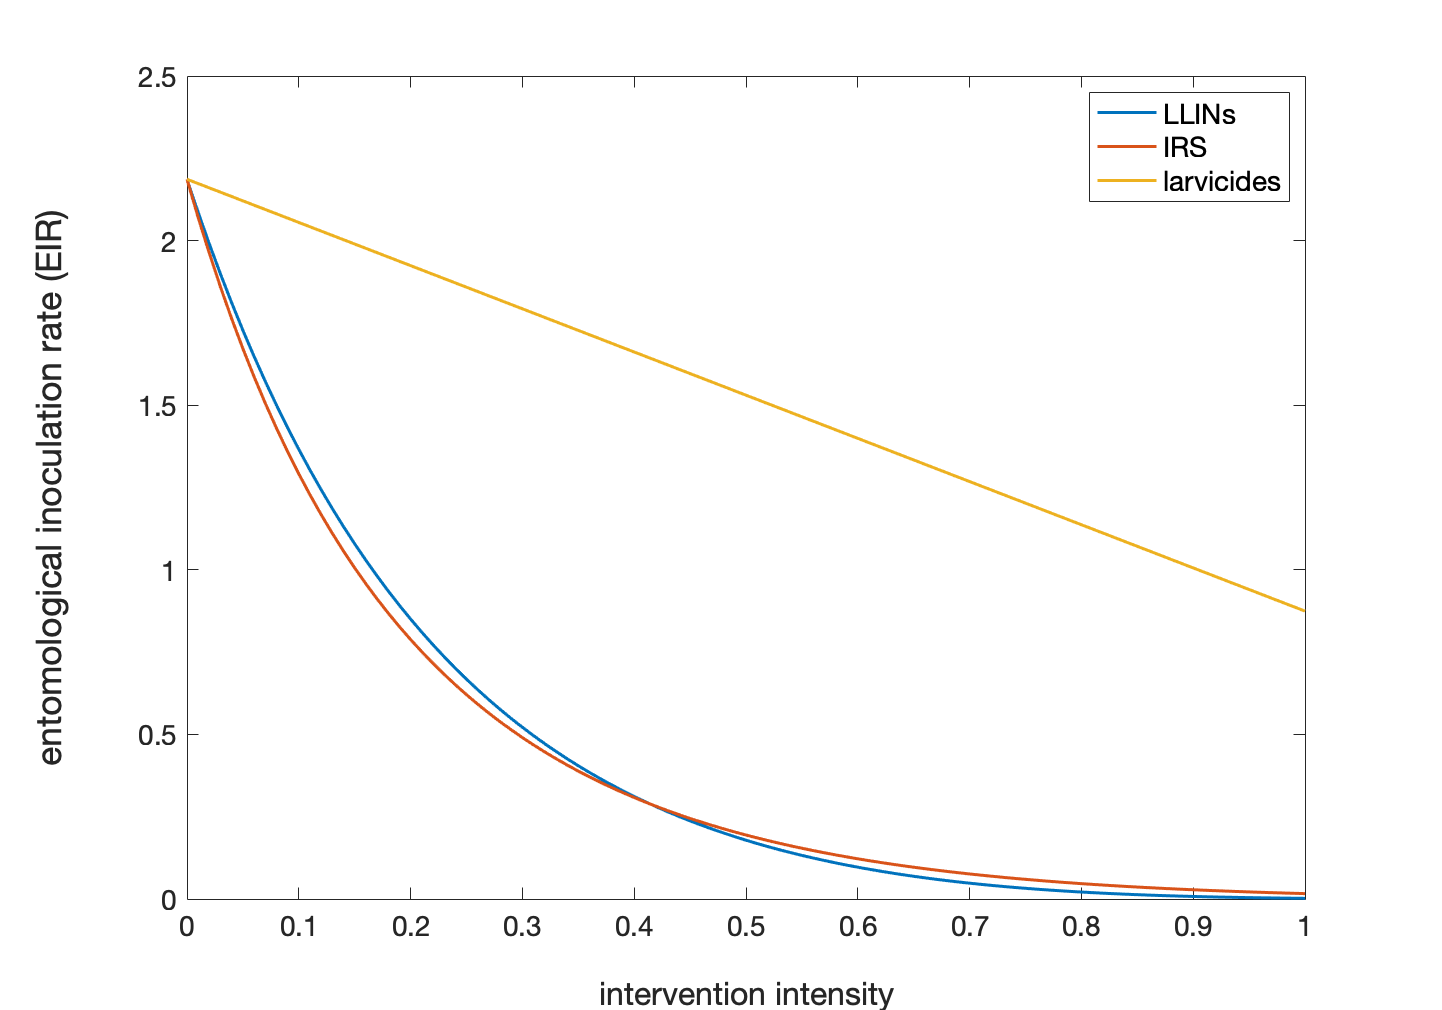
\includegraphics[height=6.7cm]{Project/Figures/VectorModel/LF/EIR.png} &
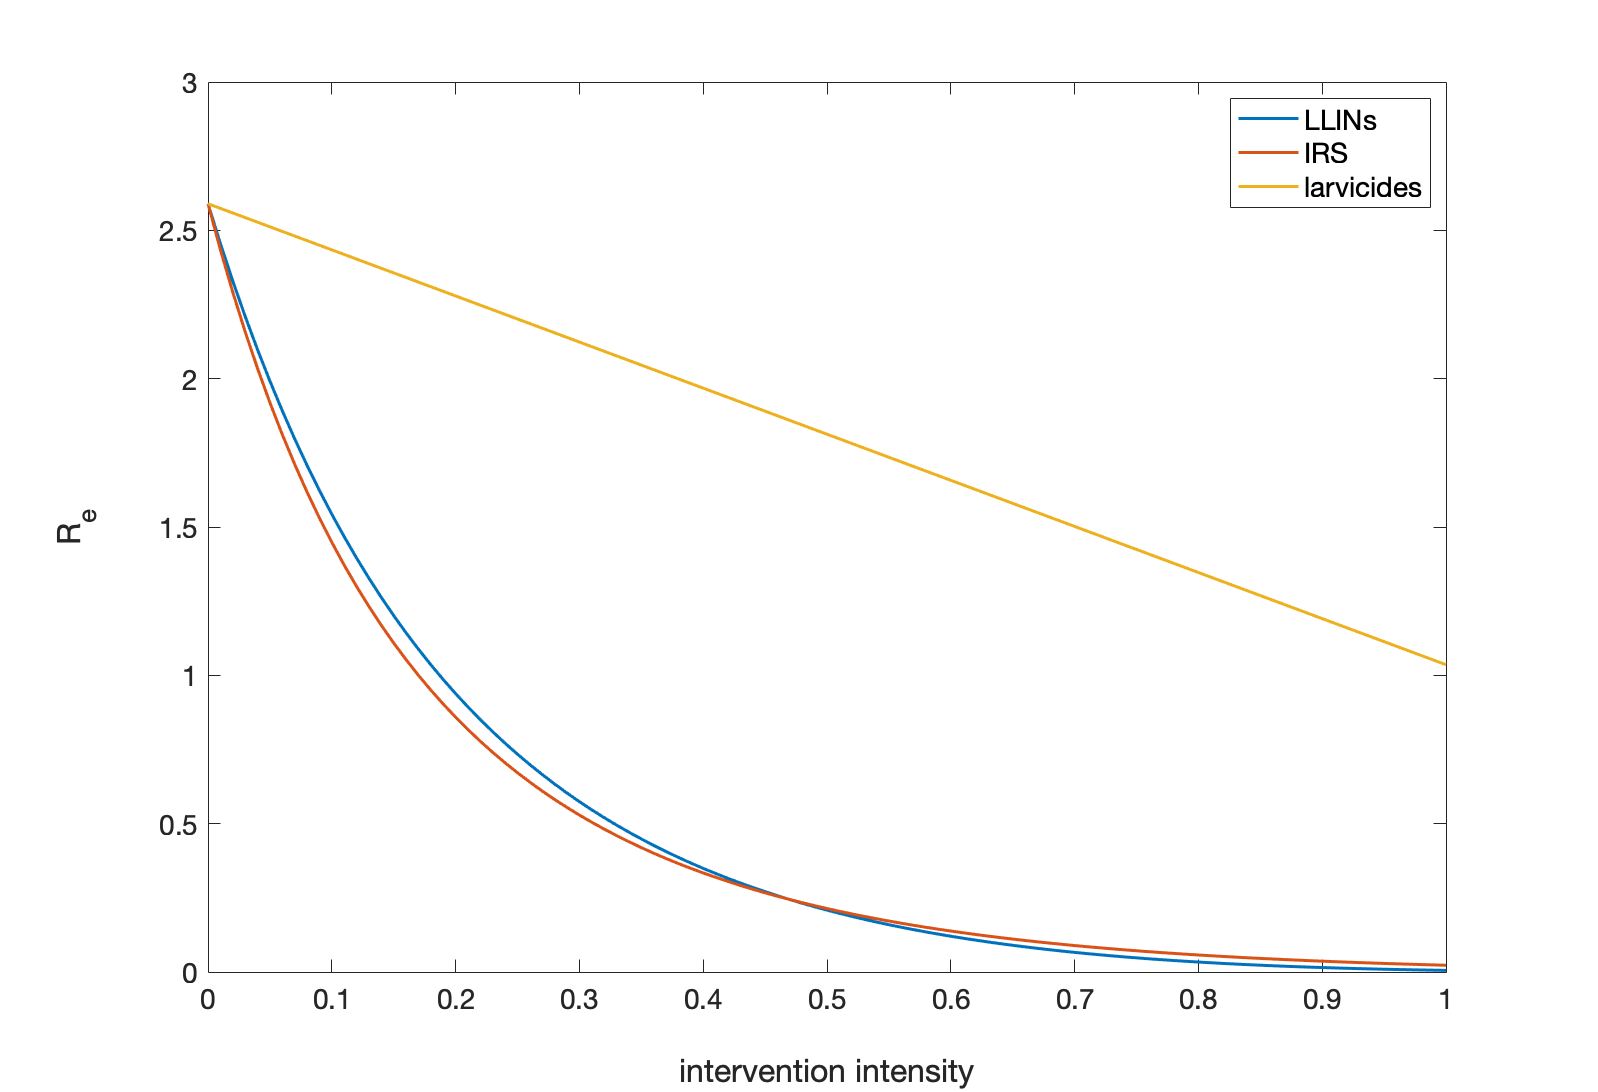
\includegraphics[height=6.7cm]{Project/Figures/VectorModel/LF/R0.png} 
\end{array}$
\caption[LF Transmission measures.]{Transmission measure comparisons for the three considered vector control interventions: LLINs (blue), IRS (red) and larvicides (yellow) from 0 to 100\% coverage. Top left: Total number of vectors in the population. Top right: Prevalence of infectious disease in vectors (not including exposed). Bottom left: Entomological inoculation rate (EIR). Bottom right: Reproductive ratio ($R_e$). For lymphatic filariasis at 40\% host mf prevalence.}
\label{fig:Epi_LF}
\end{center}
\end{sidewaysfigure} 

Having parameterised the model for LF, we can directly calculate the derived measures from Section \ref{sec:EpiMeasures} for a range of intervention intensities (see Figure \ref{fig:Epi_LF}). The emergence rate (or birth rate) of adult mosquitoes was chosen to give an $R_0$ value of approximately 2.5 in the absence of intervention \cite{Stone2014}.

In all transmission measures presented, the scale-up of larvicide coverage has the least impact and IRS and LLINs are reasonably comparable. Particularly, using larvicides doesn't decrease the prevalence of infectious vectors and has a lesser effect on the population size than either of the other two interventions. As a result, the respective decrease in key transmission measures, such as $R_e$ and the entomological inoculation rate (EIR) is only linear. Even at 100\% coverage of the adult-acting measures the vector population does not go fully extinct, and there are still very low levels of infection in the vector population. This is because IRS and LLINs are not 100\% effective at repelling or killing mosquitoes so it is still possible for a minority vectors to successfully feed, contract and potentially transmit the parasite.

The vectorial capacity is proportional to the basic reproductive number, so the results demonstrate the same effects.

\begin{sidewaysfigure}[p] 
\begin{center}$
\begin{array}{cc}
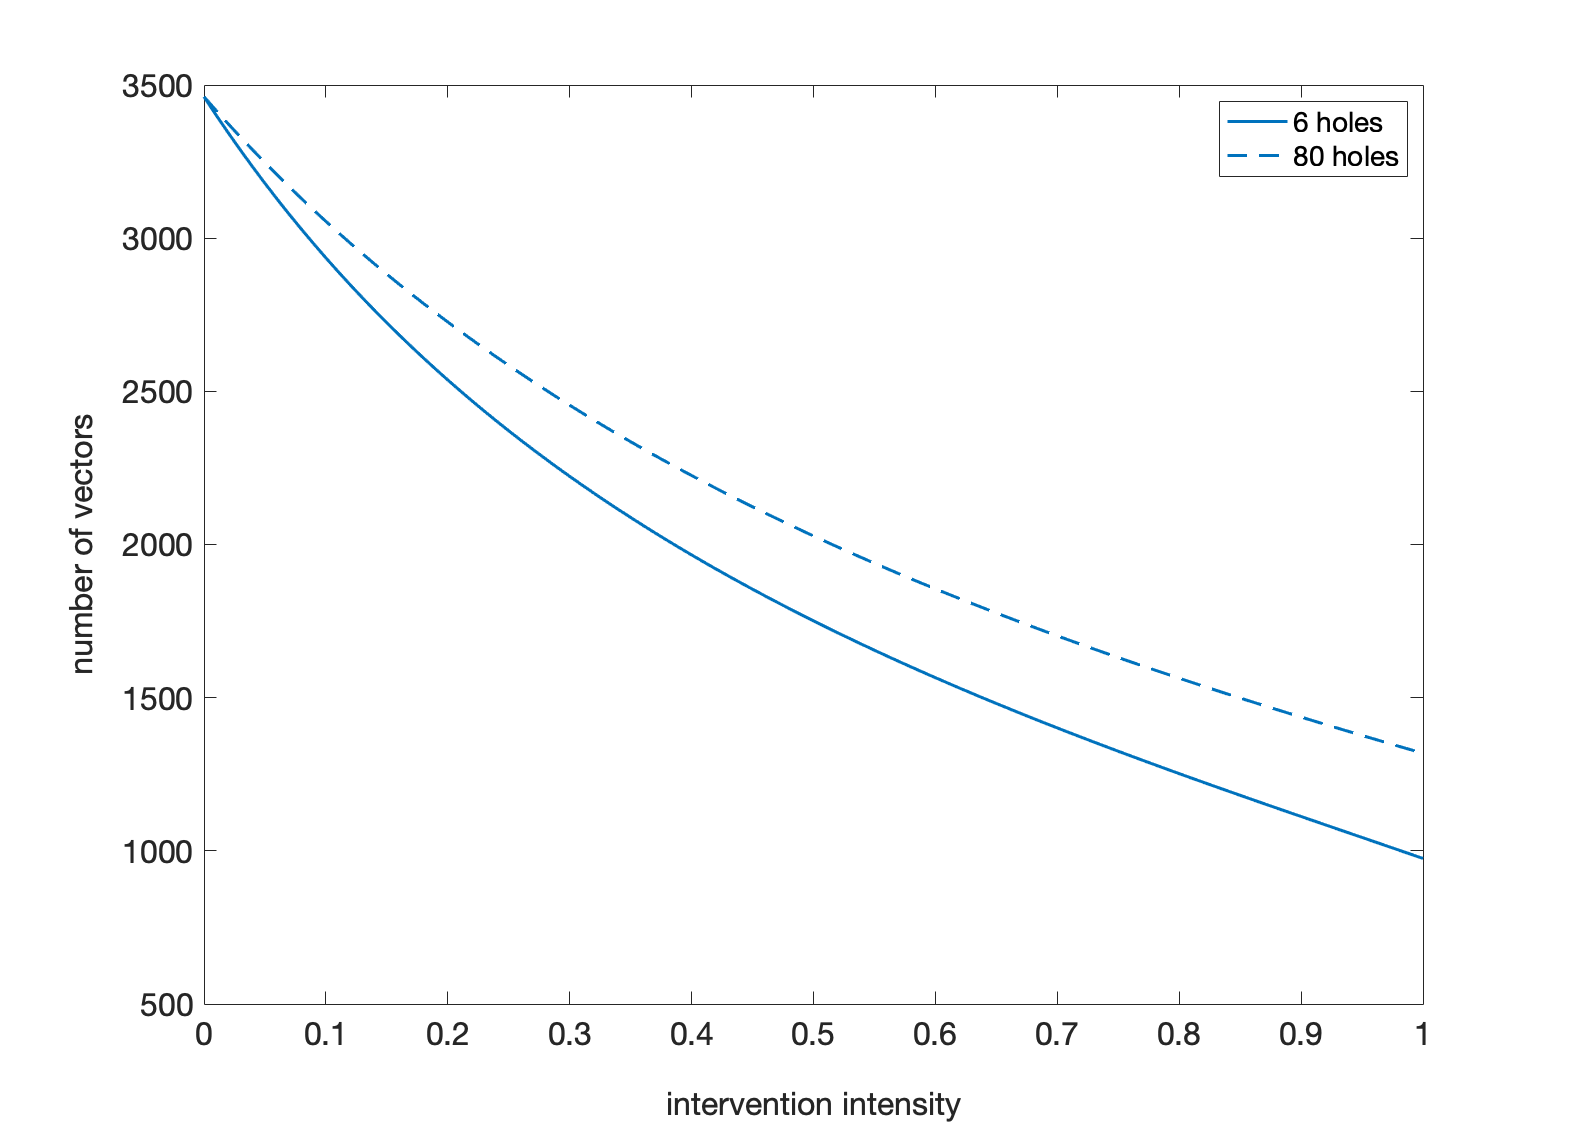
\includegraphics[height=7cm]{Project/Figures/VectorModel/LF/LLINs_holes_NumVec.png} & 
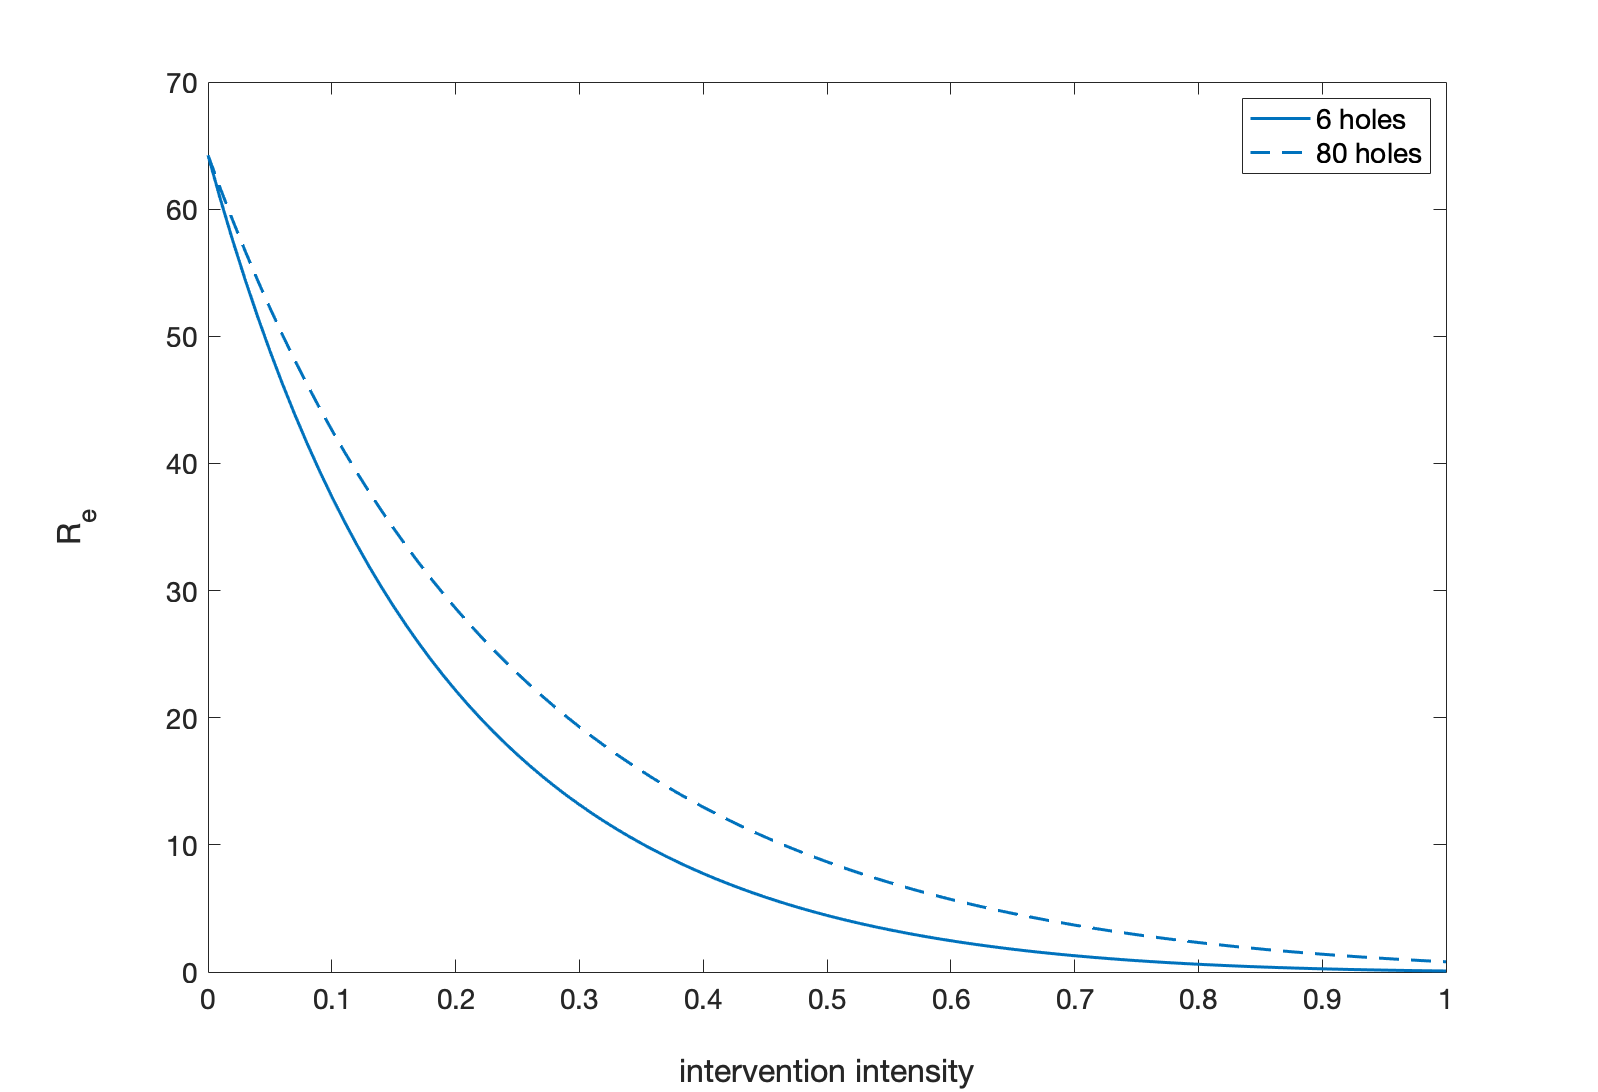
\includegraphics[height=7cm]{Project/Figures/VectorModel/LF/LLINs_holes_R0.png}
\end{array}$
\caption[LLIN integrity analysis.]{Transmission measure comparisons for LLINs of different integrity levels: 6 holes (solid) and 80 holes (dashed). Left: Total number of vectors in the population. Right: Reproductive ratio ($R_e$). For LF at 40\% host mf prevalence.}
\label{fig:holes}
\end{center}
\end{sidewaysfigure} 

In all previous plots the LLINs were assumed to be relatively new, without waning efficacy, but we can use the data presented in Section \ref{sec:VCdata} to consider how these key transmission measures change if the integrity of the nets is reduced. Figure \ref{fig:holes} shows the total number of vectors in the population and $R_e$ for a range of coverages of LLINs with 6 holes (blue, the standard assumed in previous plots) and 80 holes (red). The nets with 80 holes perform worse than the nets with 6 holes, with the biggest discrepancy in $R_e$ occurring at low-to-mid coverage levels. As the coverage level increases beyond 50\%, and the gradient flattens, the relative difference is much smaller.

\FloatBarrier

\subsection{Malaria}

Figure \ref{fig:8controls_Ma} shows how the generational distribution of the mosquito population, and the presence of infection, varies according to combinations of the three different vector control interventions (all at 50\% coverage). As with the LF results, use of larvicides has a visibly different effect to the other two interventions. As the EIP for malaria is approximately one gonotrophic cycle longer than that for LF, transmission is even more reliant on the older generations. Hence, the adult-acting interventions that shift the population distribution towards the earlier generations have an even higher impact on potential transmission.

The control combinations (bottom row Figure \ref{fig:8controls_Ma}) once again give the best outcome when adult-based control measures are combined and the addition of larvicides to any control strategy has a minimal effect on the number of infectious vectors, due to the very low number of older vectors. However, the three interventions used together is still visibly better than any other combination.

\begin{sidewaysfigure}[p] 
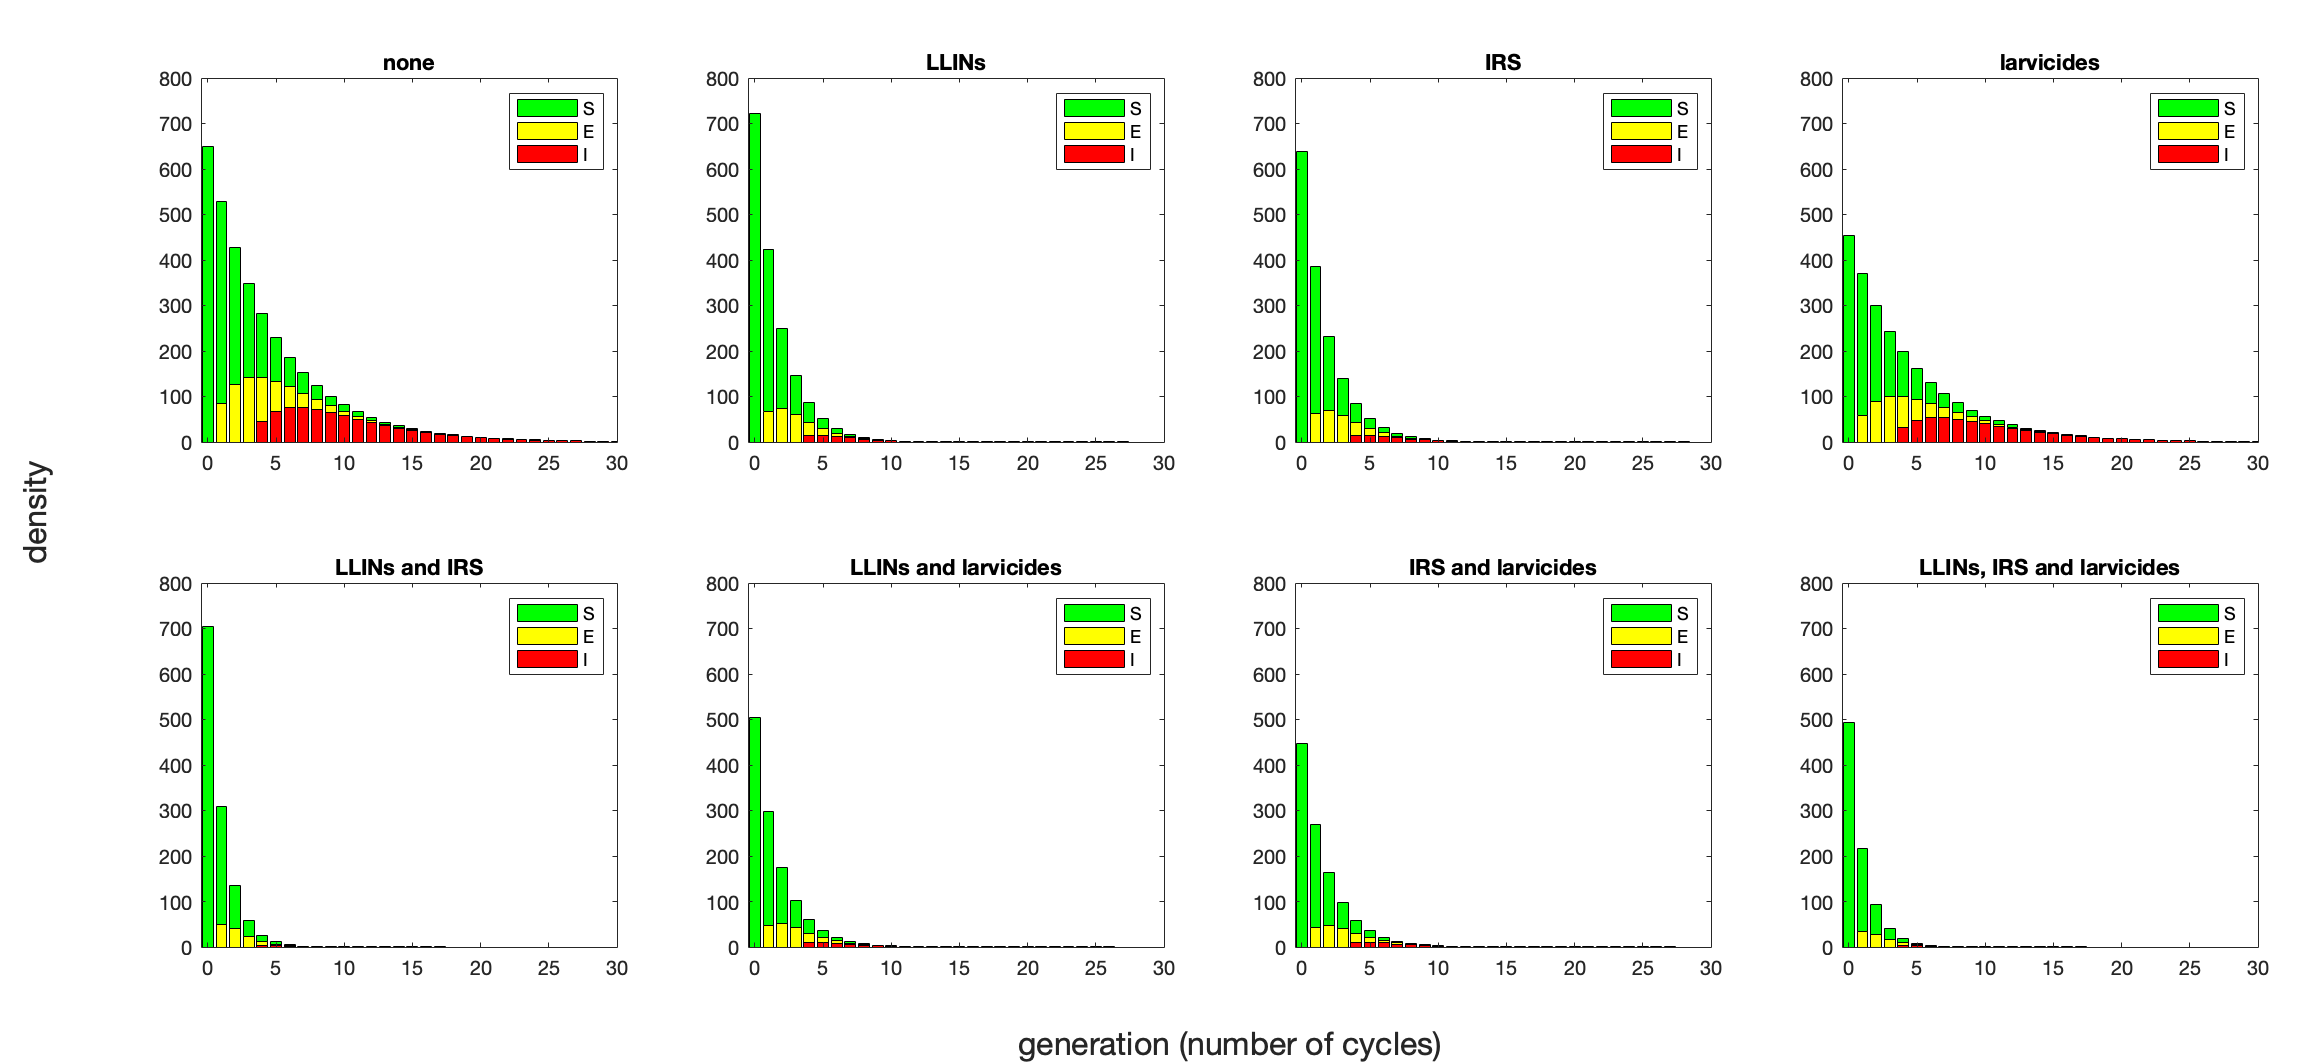
\includegraphics[height=10cm]{Project/Figures/VectorModel/Malaria/populationhist_8controls.png}
\caption[Age distribution with infection (malaria).]{Bar plots showing the age distribution of a vector population (total count, indexed by number of gonotrophic cycles completed) with a variety of combinations of vector control interventions. All interventions are assumed to have 50\% coverage. Bars are coloured by the proportion of vectors in each cycle generation that are susceptible (green), exposed (yellow) and infectious (red) for malaria at 40\% host prevalence.}
\label{fig:8controls_Ma}
\end{sidewaysfigure} 

\begin{sidewaysfigure}[p] 
\begin{center}$
\begin{array}{cc}
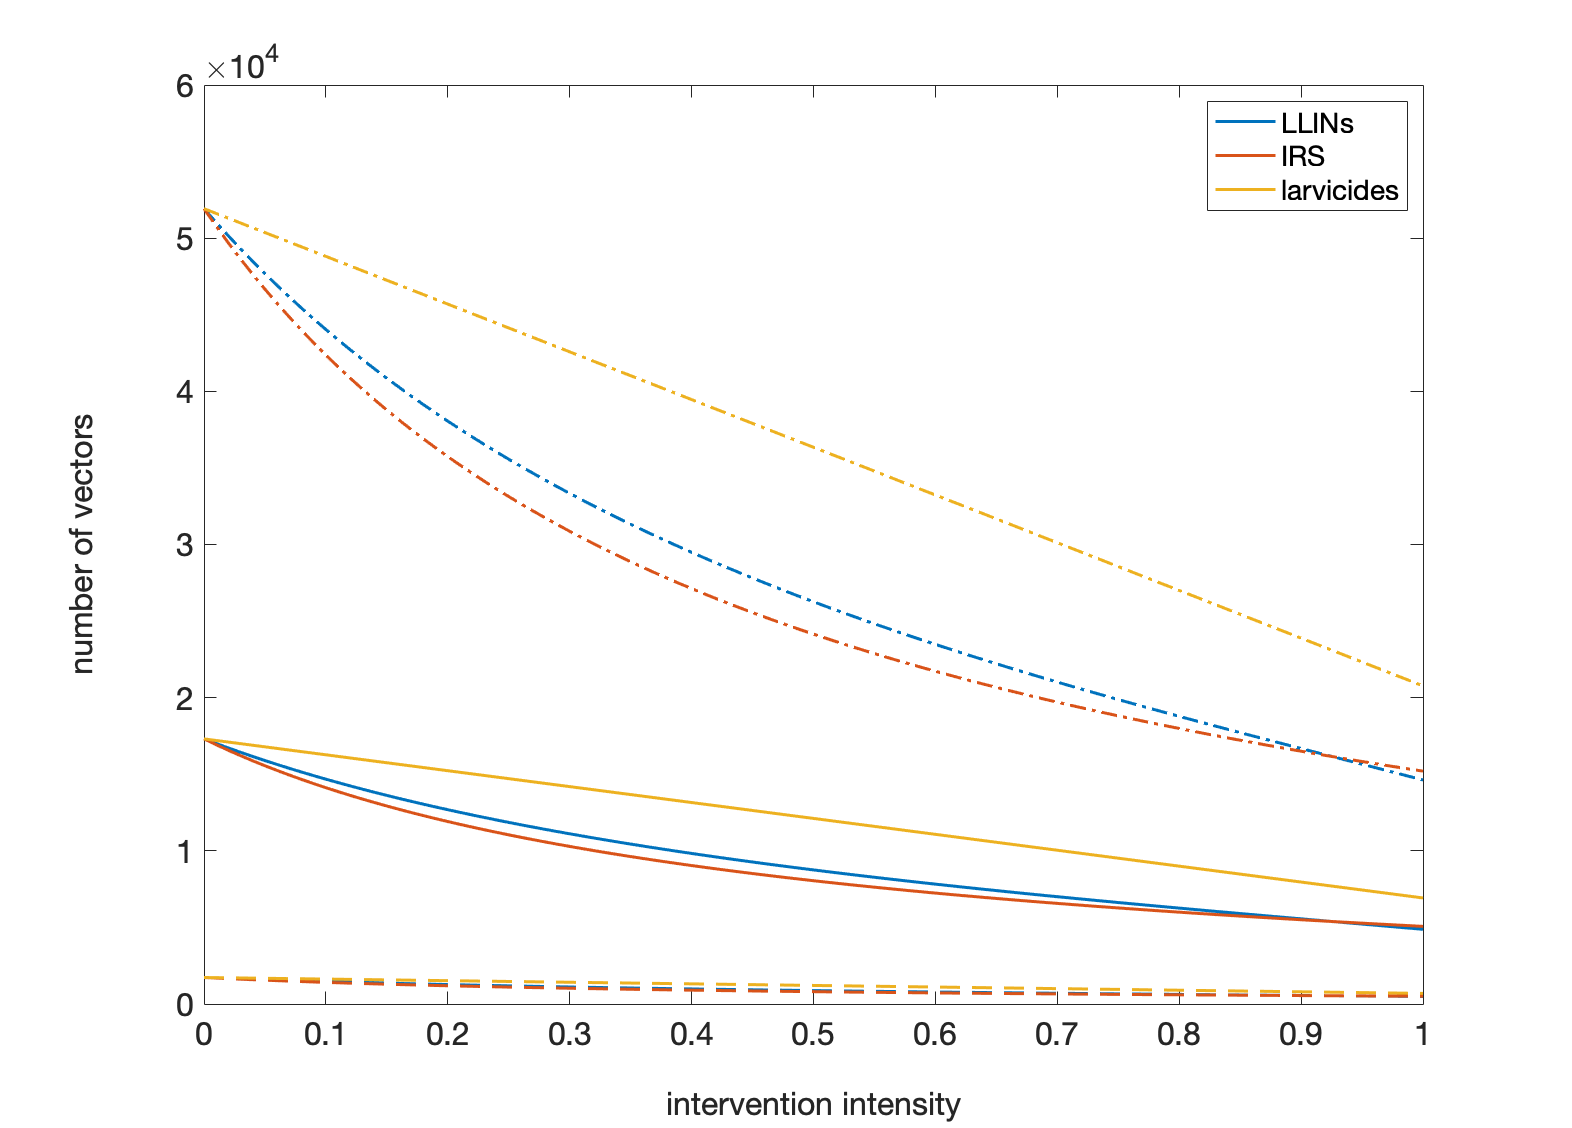
\includegraphics[height=6.7cm]{Project/Figures/VectorModel/Malaria/NumVec_lowmidhigh_new.png} & 
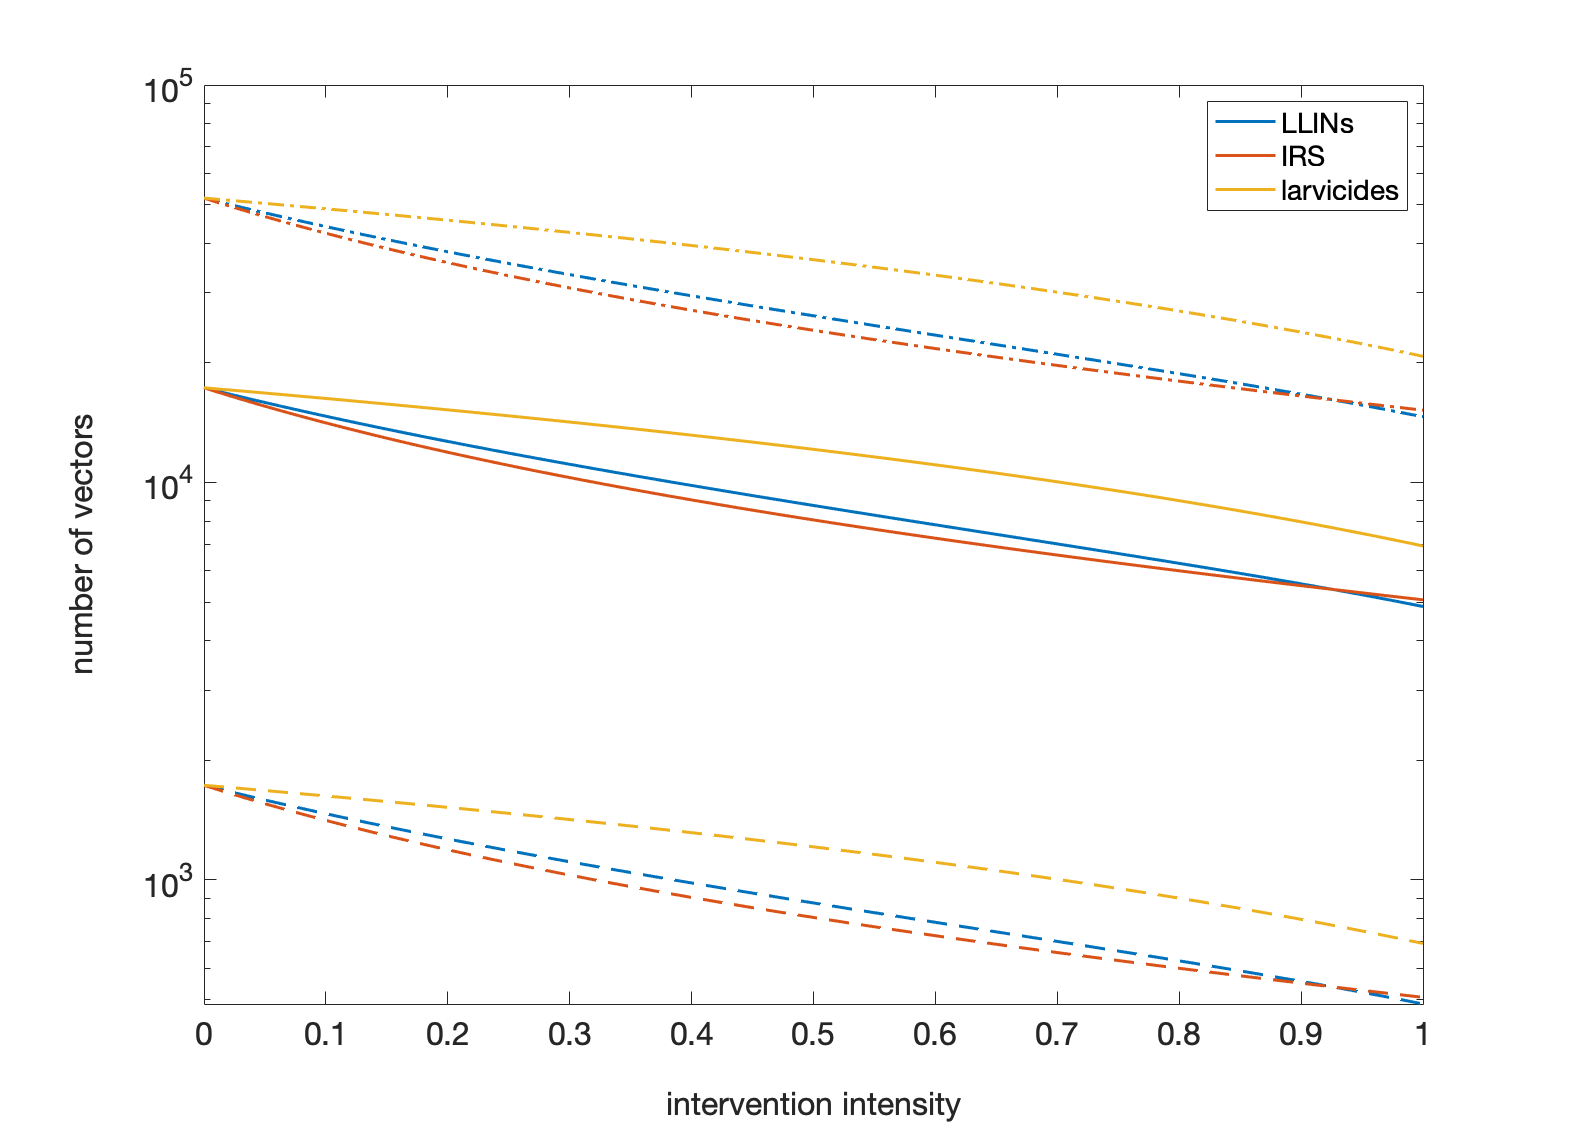
\includegraphics[height=6.7cm]{Project/Figures/VectorModel/Malaria/NumVec_lowmidhigh_log_new.png} \\
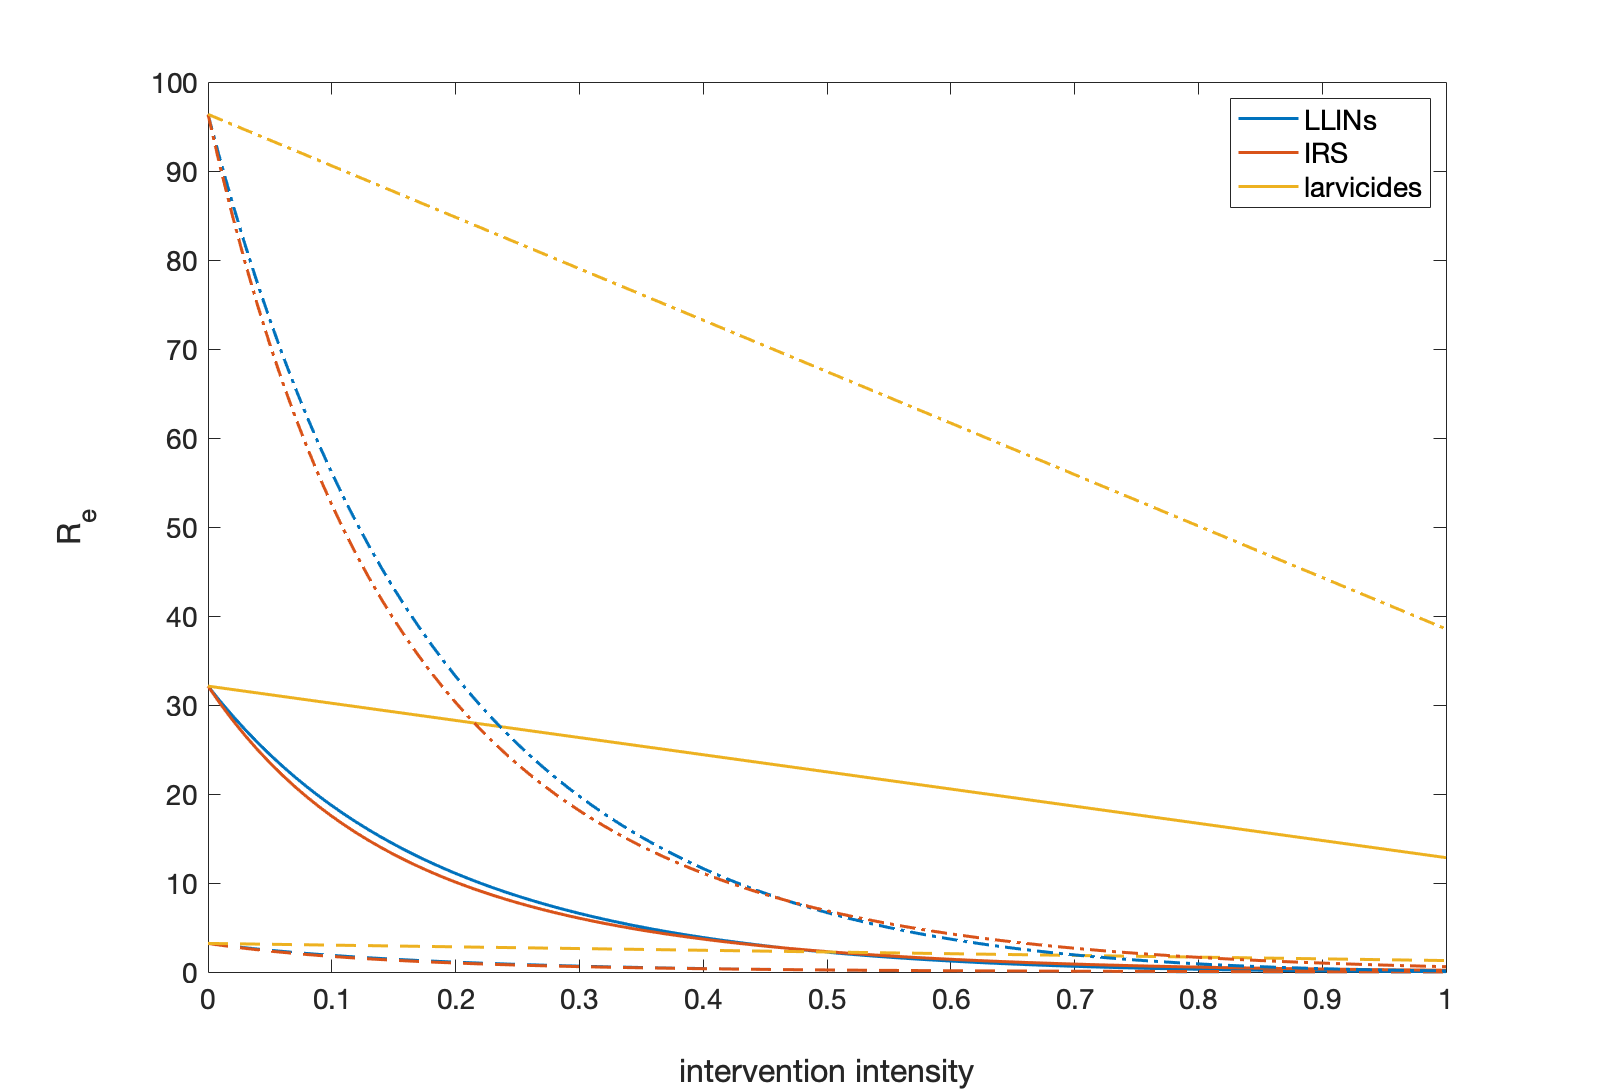
\includegraphics[height=6.7cm]{Project/Figures/VectorModel/Malaria/R0_lowmidhigh_new.png} &
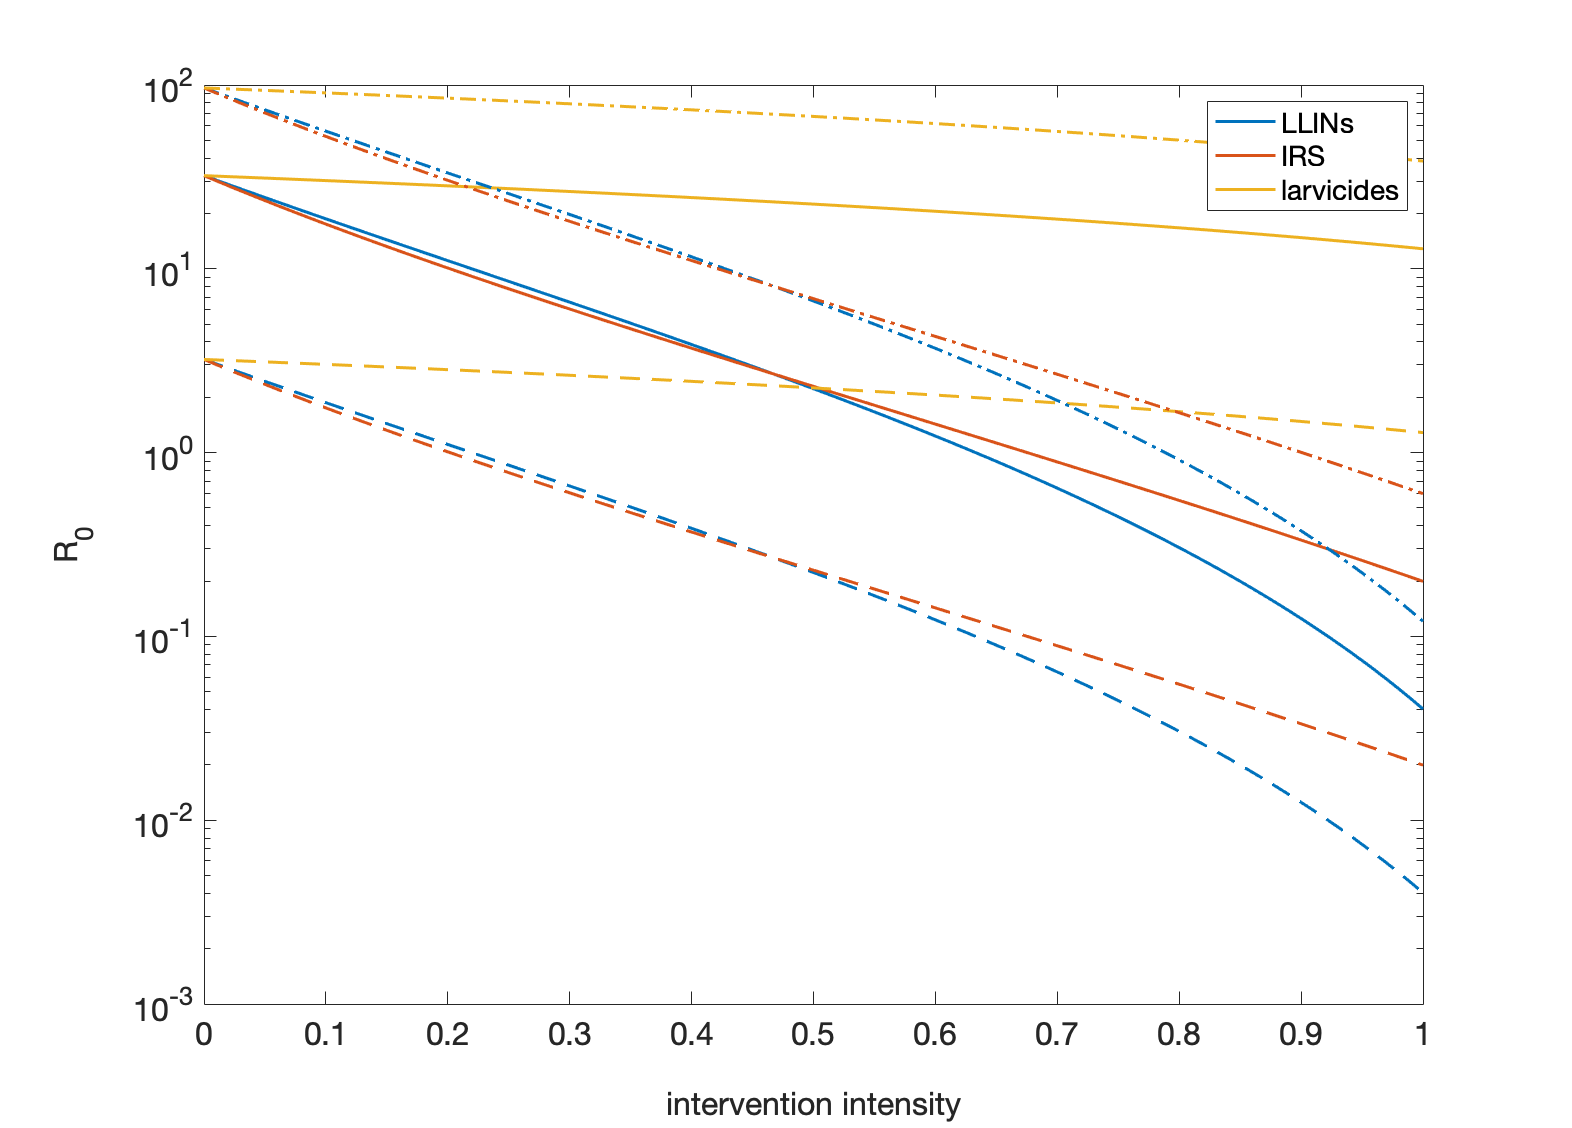
\includegraphics[height=6.7cm]{Project/Figures/VectorModel/Malaria/R0_lowmidhigh_log_new.png} 
\end{array}$
\caption[Malaria transmission measures.]{Transmission measure comparisons for the three considered vector control interventions: LLINs (blue), IRS (red) and larvicides (yellow) from 0 to 100\% coverage for high (dot-dashed), medium (solid) and low (dashed) transmission levels. Top left: Total number of vectors in the population. Top right: Total number of vectors in the population (log-scale y axis). Bottom left: Reproductive ratio ($R_e$). Bottom right: Reproductive ratio $R_e$ (log-scale y axis). For malaria at 40\% host prevalence.}
\label{fig:EpiMeasures_Ma}
\end{center}
\end{sidewaysfigure} 

When calculating the epidemiological measures, such as the EIR, for malaria it is difficult to set a fixed transmission level that is representative of malaria endemic settings, as estimates of $R_0$ in the literature vary dramatically with one review study reporting estimated values of $R_0$ ranging between one and more than 3,000 \cite{Smith2007}. Another study gives ranges between 1.3 for the lowest endemicity regions to 175.6 for the highest \cite{Gething2010}. As a result, in Figure \ref{fig:EpiMeasures_Ma} we have considered three different scenarios: high transmission (red, $R_0=400$), medium transmission (blue, $R_0=40$) and low transmission (green, $R_0=4)$. Log-scale plots are presented alongside the standard linear-scale plots to enable easier comparison between control measures for the medium and low transmission settings.

As before, the larvicides have much less impact on both the total number of vectors and the basic reproductive number than the other two adult-acting interventions. However, the log plot of the basic reproductive number shows an interesting deviation between LLINs and IRS at the higher levels of coverage that isn't visible on the linear-scale plot. This is due to the very low rate of successful feeding in the presence of LLINs (0.121), which results in much less successful feeding at high coverage due to a saturation of LLIN usage. IRS allows a higher feeding proportion (0.894 with 57\% dying post-feed) this means over 50\% of vectors seeking a blood meal will successfully feed and survive, even if every house is sprayed.

\begin{figure}[ht]
\begin{center}
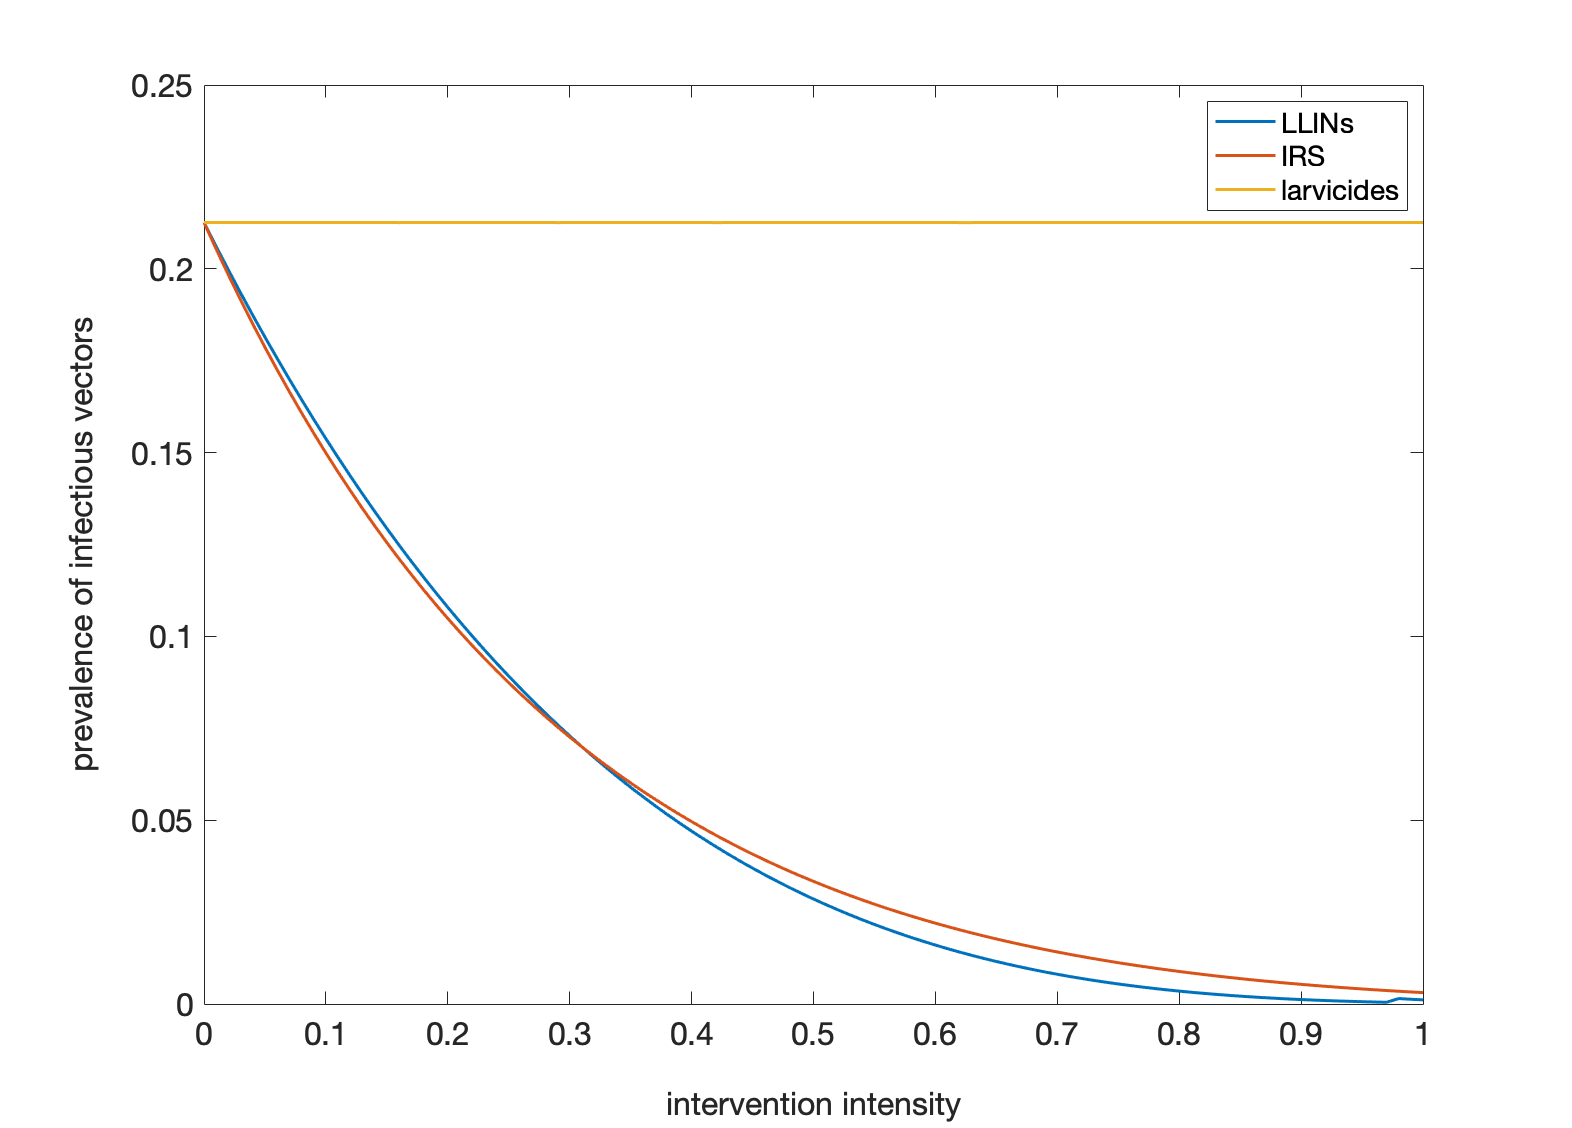
\includegraphics[height=8cm]{Project/Figures/VectorModel/Malaria/VecPrev_lowmidhigh_new.png}
\caption[Vector prevalence (malaria).]{Infectious vector prevalence comparison for the three considered vector control interventions: LLINs (blue), IRS (red) and larvicides (yellow) from 0 to 100\% coverage. For malaria at 40\% host prevalence.}
\label{fig:VecPrev_Ma}
\end{center}
\end{figure}

Figure \ref{fig:VecPrev_Ma} shows the prevalence of infectious vectors according to intervention intensity. As this is a proportional measure it is the same for all three of the low, medium and high transmission scenarios. The plot once again echoes the LF results, with larvicide coverage making no difference to vector prevalence and IRS and LLINs appearing relatively comparable throughout the range of coverage.

\subsection{Repeating effects}

Looking in closer detail at the repeating effects caused by IRS and LLINs, we can calculate the change caused in gonotrophic cycle length, and hence whether this impacts how many feeding cycles it should take for a vector to become infectious. The model parameterises the EIP in terms of number of feeding cycles, or generations, so we are mainly interested in whether changes in intervention coverage are likely to cause discrete changes.

\begin{sidewaysfigure}[p] 
\begin{center}$
\begin{array}{cc}
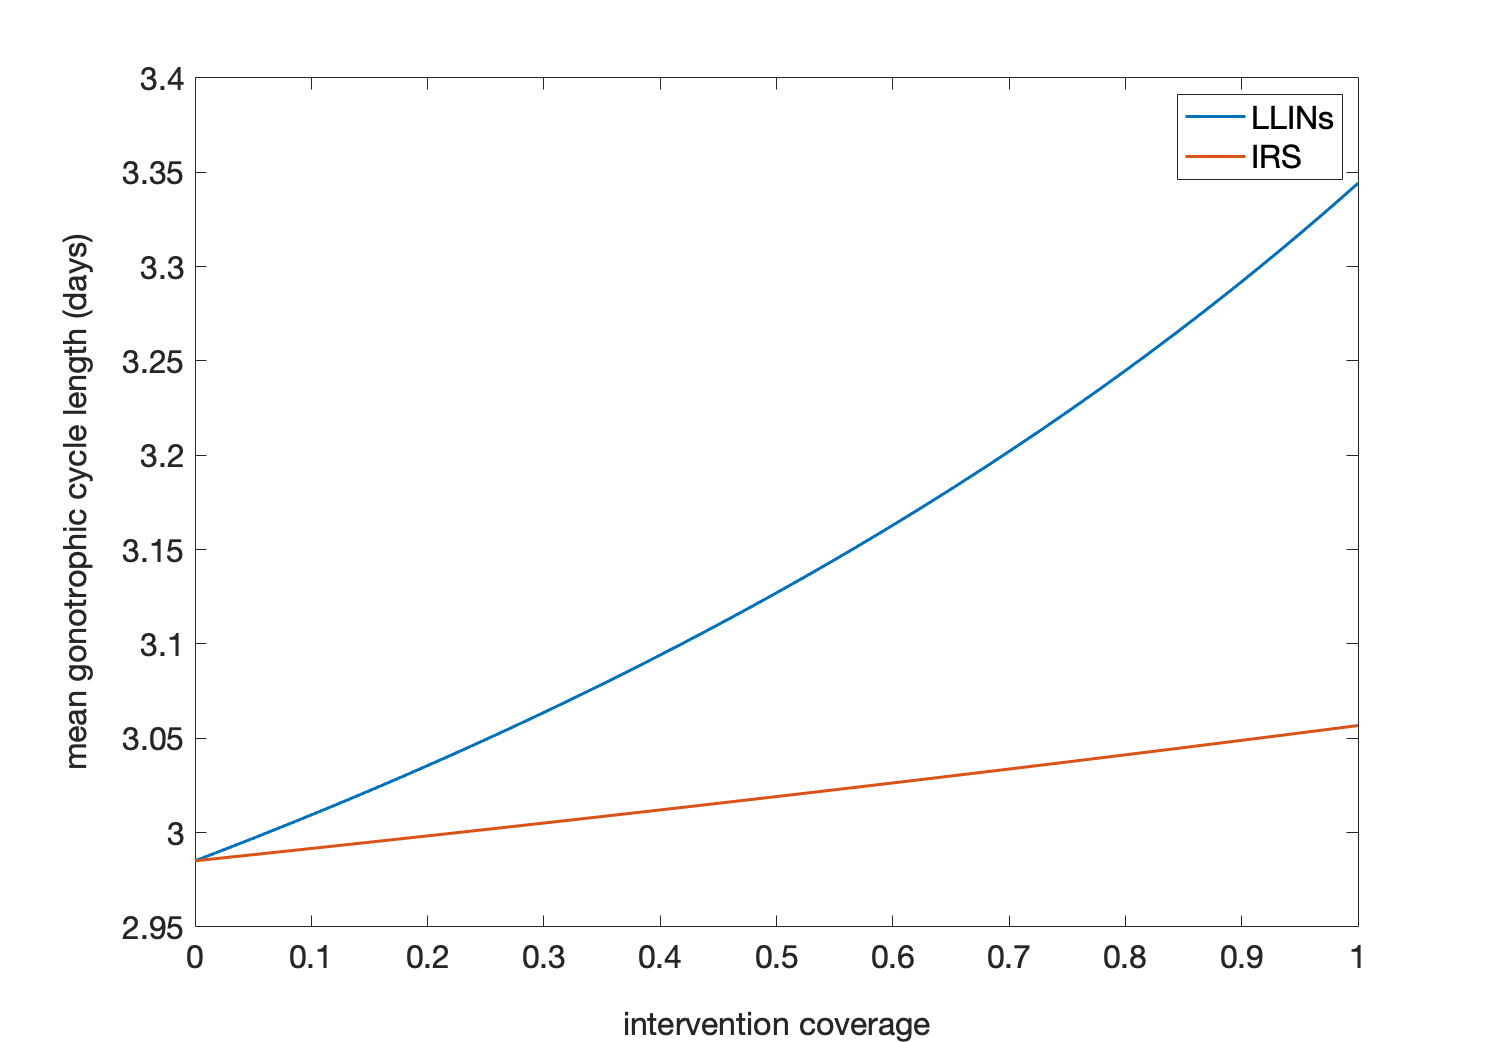
\includegraphics[height=6.7cm]{Project/Figures/VectorModel/LF/CycleLengthDays.png} & 
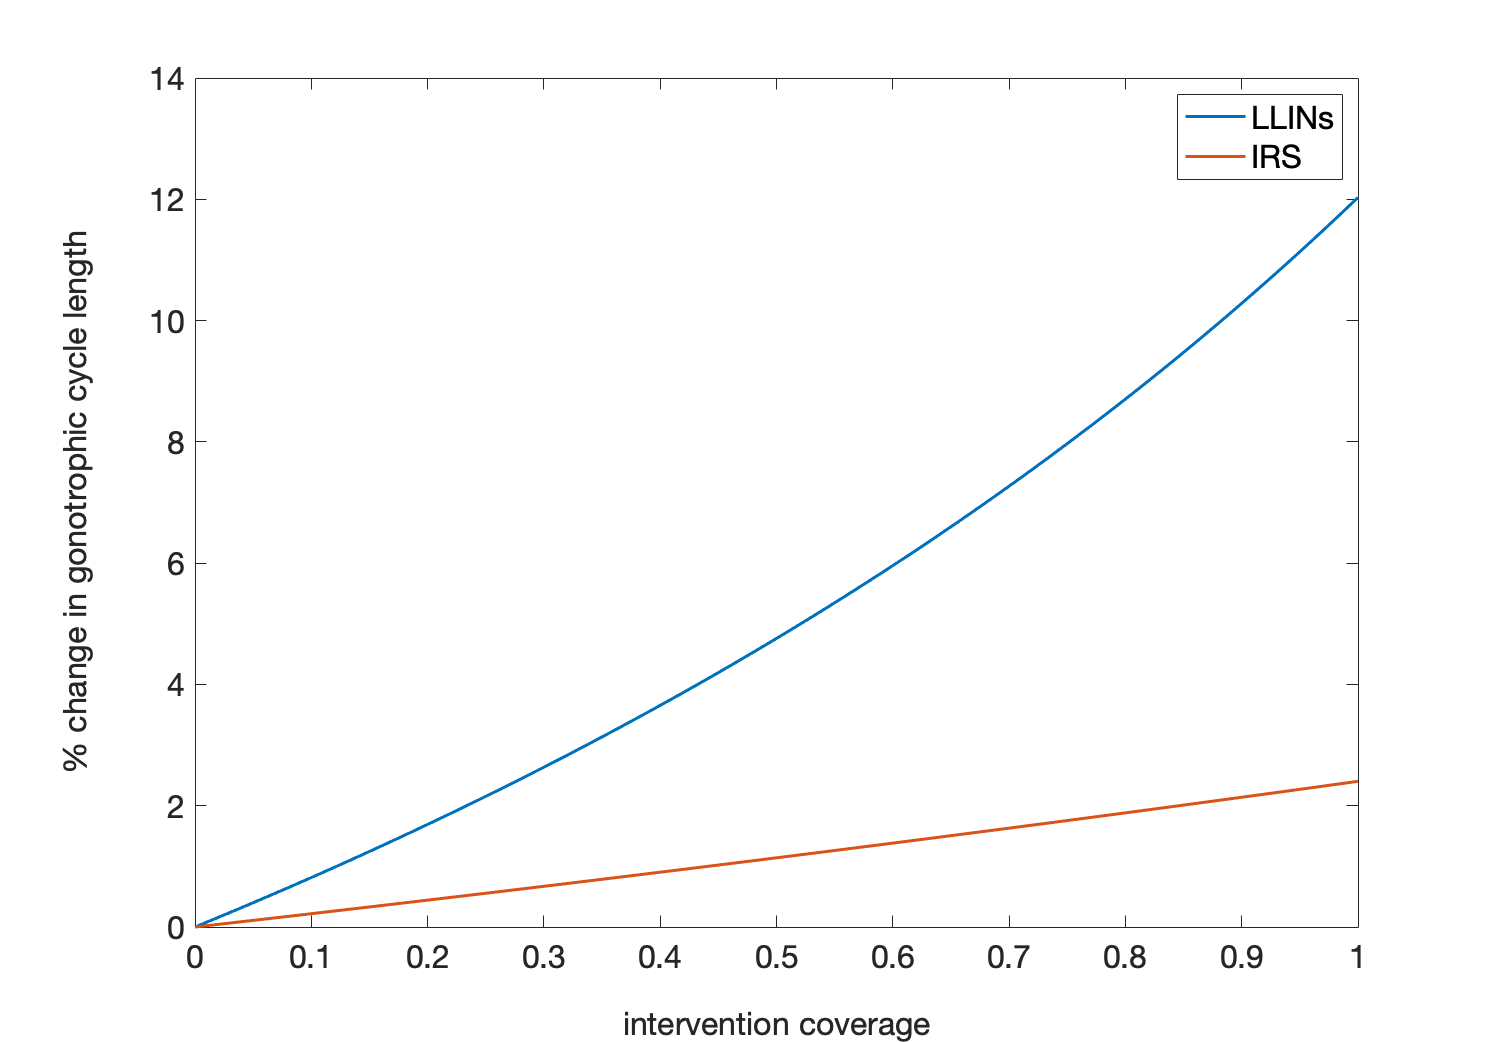
\includegraphics[height=6.7cm]{Project/Figures/VectorModel/LF/CycleLengthChange.png} \\
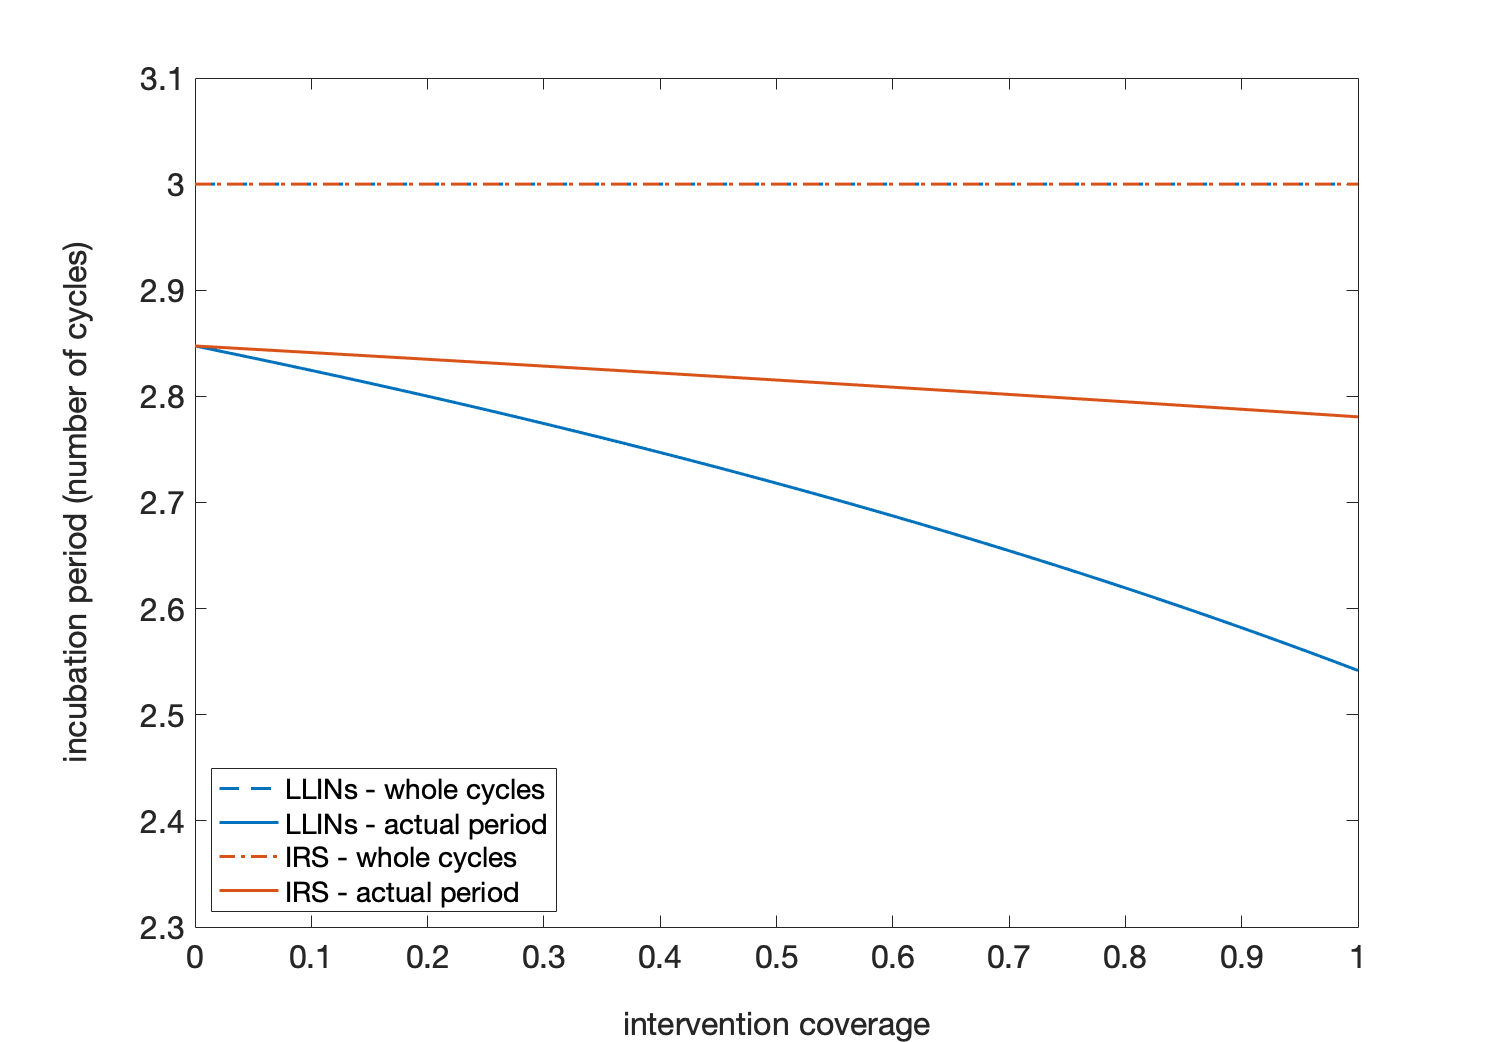
\includegraphics[height=6.7cm]{Project/Figures/VectorModel/LF/NumberCycles.png} &
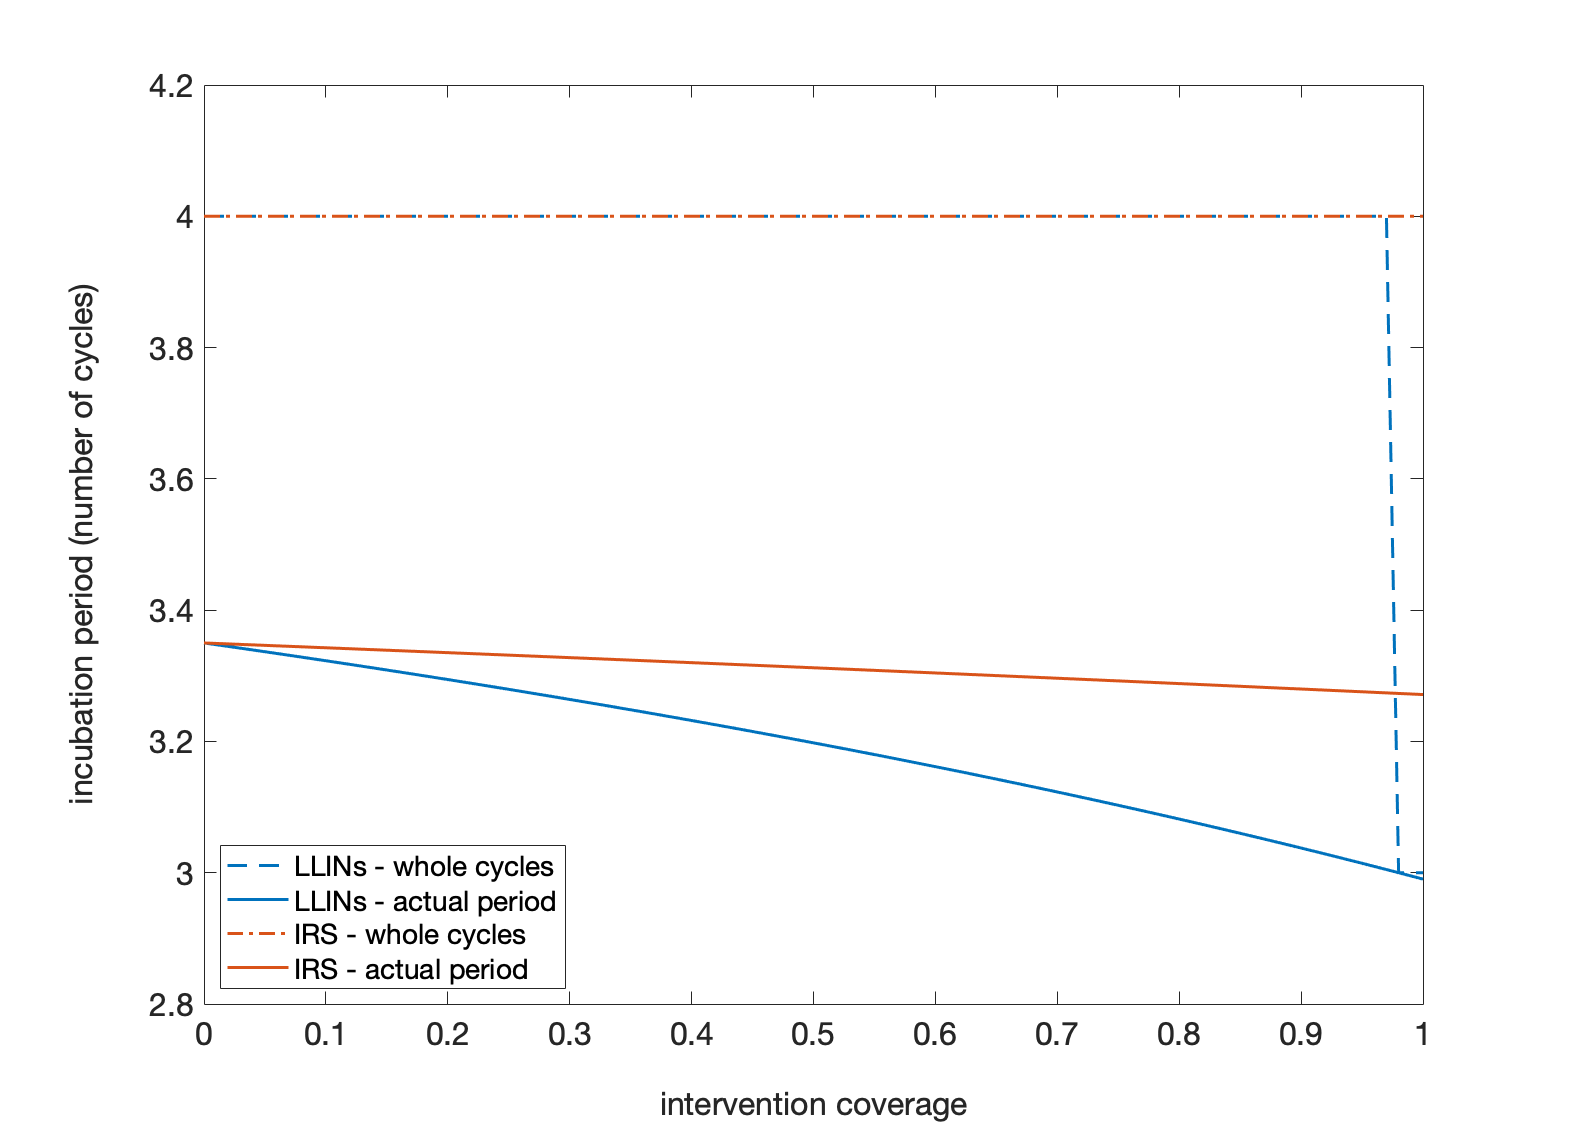
\includegraphics[height=6.7cm]{Project/Figures/VectorModel/Malaria/NumberCycles.png}
\end{array}$
\caption[Impact of repeating on gonotrophic cycle length.]{Cycle length plots for vector control interventions with repeating effects: LLINs (blue) and IRS (red). Top left: Mean change to gonotrophic cycle length (days). Top right: Percentage change in gonotrophic cycle length (\%). Both plots on the top row are independent of disease. Bottom left: Impact on incubation period in terms of the number of fractional (solid) and complete (dashed) cycles before infectiousness for lymphatic filariasis. Bottom right: Impact on incubation period in terms of the number of fractional (solid) and complete (dashed) cycles before infectiousness for malaria.}
\label{fig:cycles}
\end{center}
\end{sidewaysfigure} 

Figure \ref{fig:cycles} reiterates what we already saw in Figure \ref{fig:8controls_LF}, that LLINs have a much stronger repeating rate and this causes a larger increase in the gonotrophic cycle length. IRS can only cause at maximum just over a 2\% increase in mean cycle length, but high coverage of LLINs could lead to up to a 12\% increase. For LF (Figure \ref{fig:cycles} bottom left) the mean number of cycles required to pass through the EIP is around 2.85 in the presence of no interventions. A 12\% increase in cycle length results in an EIP which is still more than 2.5 cycles, hence three cycles are still required before a vector will be able to perform an infectious bite. Even 100\% coverage of LLINs is not sufficient to decrease the number of cycles required to reach infectivity.

For malaria (bottom right) LLINs are capable of bringing the EIP down from four cycles to three cycles, but only at very high coverage levels (greater than 95\%). As achieving 95\% LLIN coverage in practice is an unrealistic goal, this means that for the purposes of our results, the repeating effect has no change on the effective length of the incubation period in terms of generations of feeding, hence it is reasonable to take this parameter as fixed in the model for the purposes of our results. 

\subsection{Elimination settings}

As in Chapter \ref{chap:ELIM}, we are interested in elimination settings for LF, where we are either close to, or have achieved, a human prevalence of less than 1\% mf. Here we consider a setting where this reduction in prevalence has been caused largely by mass drug administration (MDA), rather than vector control measures. The impact of this on the vector dynamics can be simulated by considering a setting with the same vector to host ratio (or the same adult vector emergence rate) but a lower host prevalence. We are then interested in how using vector control measures will impact onward transmission.

\begin{sidewaysfigure}[p]
\begin{center}$
\begin{array}{cc}
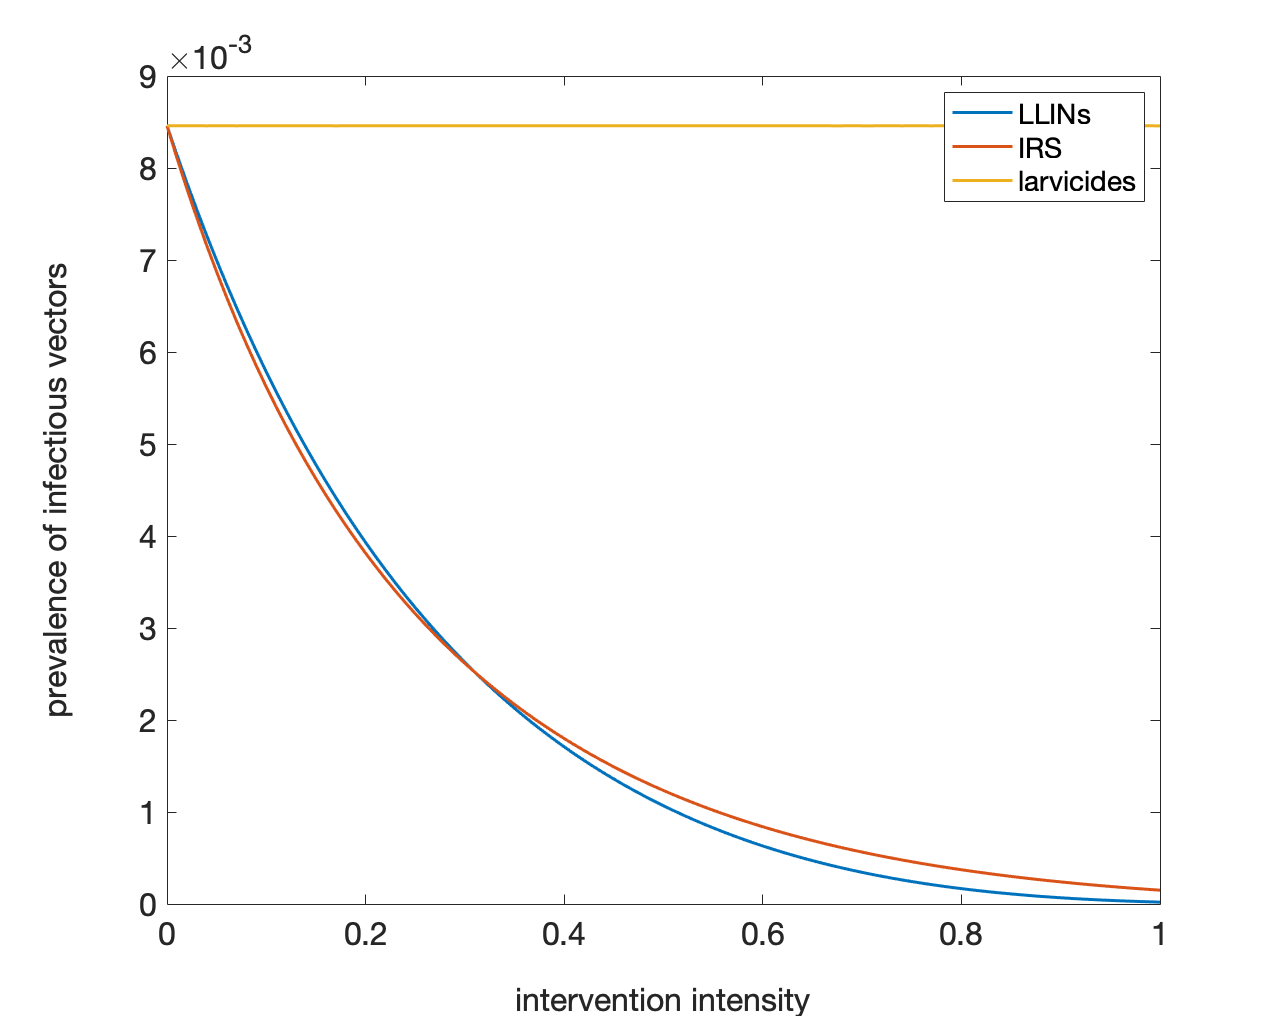
\includegraphics[height=8.5cm]{Project/Figures/VectorModel/LF/VecPrev_1mf.png} &
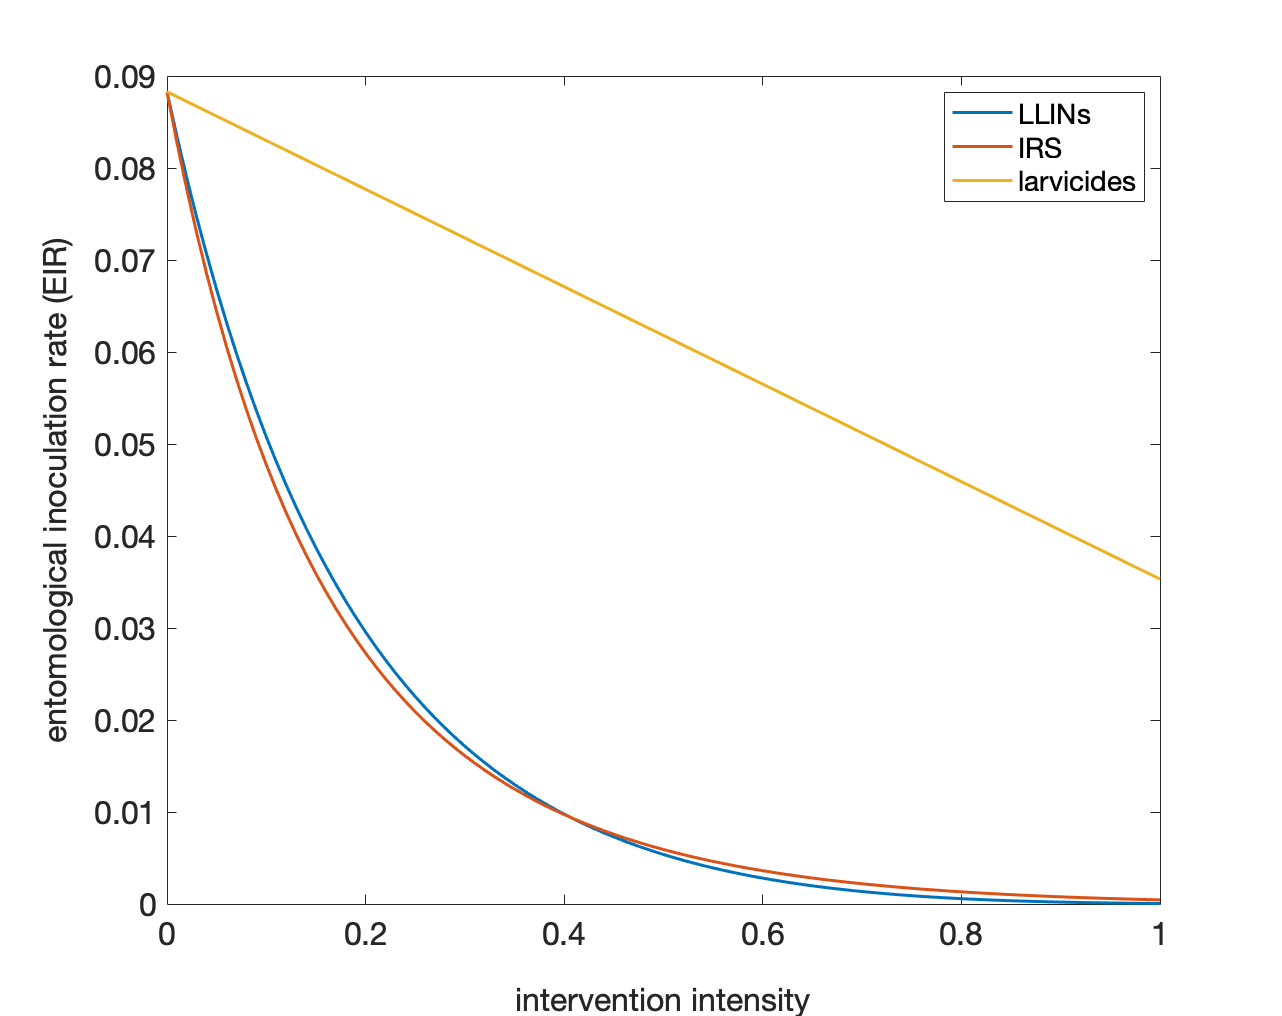
\includegraphics[height=8.5cm]{Project/Figures/VectorModel/LF/EIR_1mf.png}
\end{array}$
\caption[LF transmission measures at EPHP prevalence levels.]{Repeats of vector control intervention plots for the prevalence of infectiousness in vectors (left) and EIR (right) for LF with a host mf prevalence of 1\%. Other measures, including $R_e$, number of vectors in the population and vectorial capacity, are unchanged by the reduction in host prevalence.}
\label{fig:Elim_LF}
\end{center}
\end{sidewaysfigure} 

Transmission measures such as the basic reproductive number are independent of host prevalence, as they are defined based on one average infectious individual. However, the prevalence of infectious vectors and associated measures such as the EIR are substantially reduced by a reduction from 40\% to 1\% host prevalence (Figure \ref{fig:Elim_LF}).

When low host prevalences have been achieved it is highly important to maintain, and if possible improve on, these gains. In particular, adult-acting vector control measures and the impact they can have on $R_e$ could be vital in the final phases of elimination programs. 

\subsection{The Gambia}

Following on from the evidence of elimination discovered in The Gambia in the absence of MDA, I used the host infection process described in Section \ref{sec:Host} to investigate whether the model could achieve a prevalence of less than 1\% mf using just LLINs. I considered an equilibrium host mf prevalence of 50\%, which is reflective of measured mf levels in The Gambia in the 1950s, and then calculated the trend in human infection across ten years of consistent LLIN usage.

Figure \ref{fig:WM} shows the mean worm burden (W) and microfilaria count per 20$\mu$l of blood (M) decreasing over a ten year period in the presence of 40\% (left) and 80\% (right) LLIN coverage. There is a noticeable difference between the two levels of intervention and the decreasing mf levels appear to be reaching a plateau by the 10 year mark in both instances.

\begin{figure}[!ht]
\begin{center}$
\begin{array}{cc}
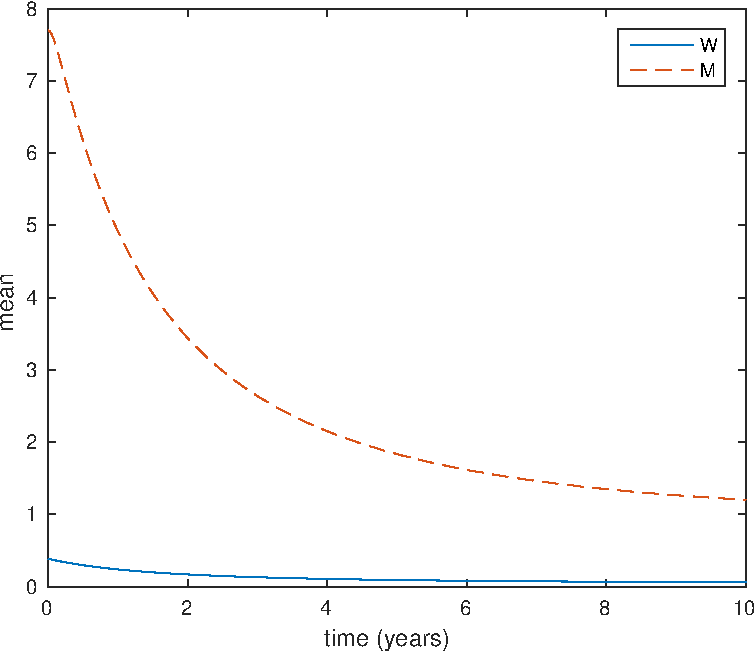
\includegraphics[height=5.8cm]{Project/Figures/VectorModel/LF/WM_1950s_omega=40per.pdf} &
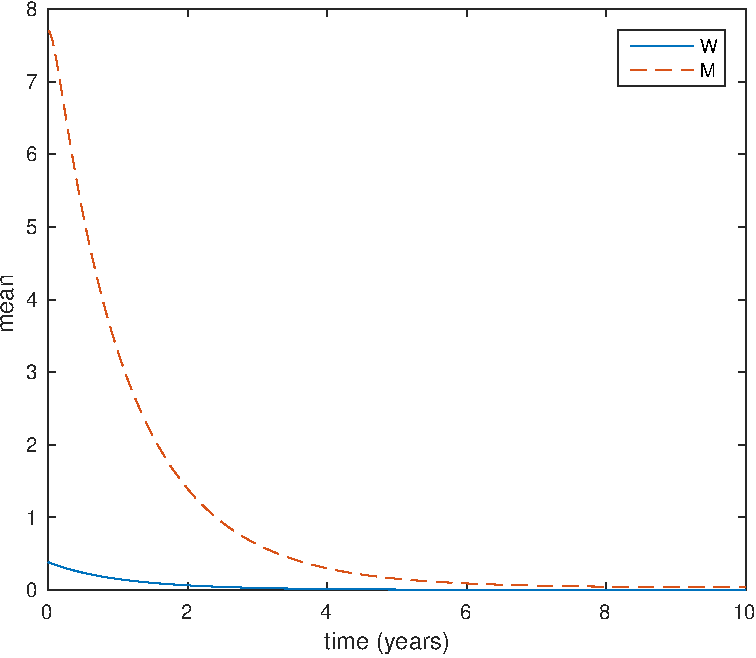
\includegraphics[height=5.8cm]{Project/Figures/VectorModel/LF/WM_1950s_omega=80per.pdf}
\end{array}$
\caption[LLIN impact over time (LF).]{Mean adult worm burden (W, blue solid) and mf count per 20$\mu$l of blood (M, red dashed) over ten years of LLIN usage at 40\% coverage (left) and 80\% coverage (right). Considering an equilibrium mf prevalence of 50\%, to reflect 1950s prevalence in The Gambia.}
\label{fig:WM}
\end{center}
\end{figure} 

Due to these apparent diminishing returns, we now consider the net benefit of 10 years of LLIN usage for a range of coverage, still given a starting mf prevalence of 50\% (Figure \ref{fig:10yrLLIN}). Looking at both the host and vector prevalences, we see the most substantial gains can be made by increasing coverage up to around 60\%; beyond this point increases in LLIN coverage have a much smaller relative effect. However, a coverage of 80\% or higher would be required to get host mf prevalence to below 1\% in this time period.

\begin{figure}[!ht]
\begin{center}
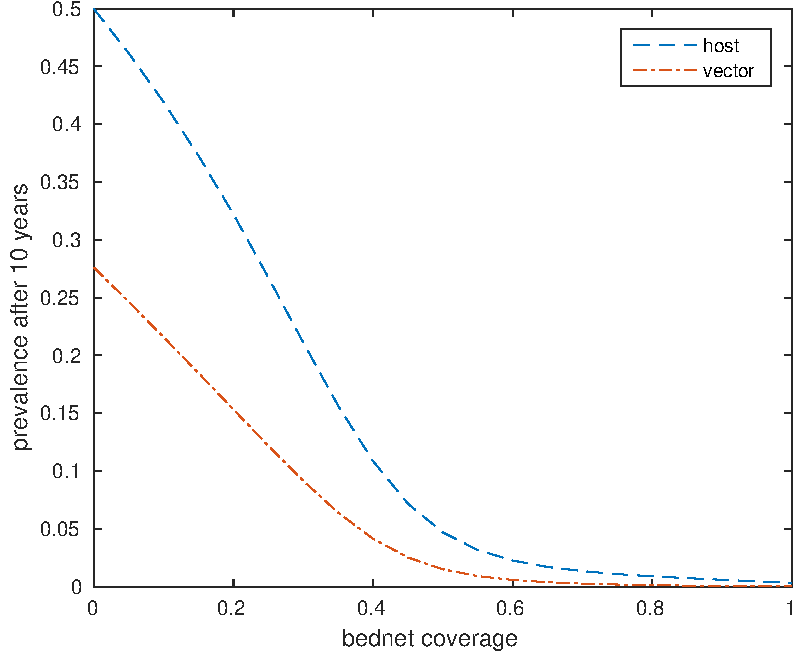
\includegraphics[height=8.5cm]{Project/Figures/VectorModel/LF/10yearprev_1950s_bednets.pdf} 
\caption[LLIN impact over 10 years (LF).]{Prevalence of LF in the host (blue dashed) and vector (red dot-dashed) after 10 years of LLIN usage for coverage between 0 and 100\%, starting at 50\% baseline mf prevalence.}
\label{fig:10yrLLIN}
\end{center}
\end{figure} 

\FloatBarrier

\section{Discussion}

The results presented in this chapter have used the explicit equilibrium solution of a gonotrophic cycle model for mosquito dynamics. Primarily the aim was to investigate how different vector control measures could change mosquito population structure and hence the potential effect on transmission of vector-borne diseases such as LF and malaria. We were also interested in the role long-lasting insecticidal nets may have played in the reduction of LF prevalence to below EPHP levels in The Gambia. We found that adult-acting vector control measures are likely to have a much greater effect on transmission than larval-based interventions. In particular, LLIN and IRS both have a compounded effect due to the repelling action reducing transmission both from host to vector and from vector to host. Areas that are co-endemic for malaria and LF, or other mosquito-borne diseases such as dengue, could especially benefit from adult-acting vector control. 

Considering the longitudinal usage of LLINs, the majority of reductions in mean worm burden and mf prevalence are achieved within 5 years of implementation. Even for relatively low LLIN coverage (40\%) a plateau begins to emerge around 10 years after implementation. Whilst we show that substantial reductions in mf prevalence could be caused by LLIN usage, we find that coverage may have to be unrealistically high (greater than 80\% of individuals sleeping under nets) to reproduce the results seen in The Gambia in the absence of other factors. This implies that LLINs may have played an important role in reducing prevalence across this over 50 year period, but that other environmental and social factors are also likely to have contributed to reducing transmission.

We assumed a number of things in the construction of this model, including a fixed EIP in the mosquito, that there is no impact of infection of vector fitness and that vector mortality remains constant with age. This last assumption is consistent with current understanding of wild mosquito populations; although senescence is observed in laboratory mosquitoes, wild mosquitoes are expected to die long before they can exhibit any substantial deterioration with age \cite{Ryan2015}. We also assumed that vector control interventions were maintained at the same coverage level across time, with no waning effects, which would be logistically difficult and expensive to achieve.

It is also important to remember that scale-ups in use of insecticides to combat transmission can result in wide-spread insecticide resistance and behavioral changes in sleeping conditions can lead to changes in biting behavior \cite{Fornadel2010,Weill2003}. These factors have the potential to undermine progress made using vector control measures, and in particular evidence of this has been seen in a number of malaria control programs \cite{Ranson2016,Hemingway2016,Toe2014}.

This model has been developed based on vector models in the malaria literature and hence makes no consideration of the parasite density dependent infectivity we expect to see for LF. In medium to high prevalence settings we would expect the probability of a mosquito becoming infected during an infectious blood meal to increase if the host has a higher worm burden. Future work could expand on the current model by considering the infection probability from host to vector as dependent on the mean filarial load, but would need more detailed data to parameterise this relationship. However, even with these limitations, considering the vector dynamics still provides important insight into how vector control measures could be explicitly described in established LF models.

Our results cover a range of high and medium transmission settings, briefly touching on a low prevalence setting of 1\%, but we do not consider host prevalences of less than 1\% mf. In the absence of explicit inclusion of the mating requirements for filarial worms, we would not expect to see the breakpoint described in Chapter \ref{chap:ELIM}. As this break point is often estimated as being below 1\% mf prevalence, we wouldn't expect this exclusion to have substantial impact on our presented results, although it is likely that vector control could prove a vital tool in the final stages of elimination.

As more countries begin to bring disease levels down towards the 1\% mf prevalence range, and target passing TAS, the key questions of importance change. Here we have presented a first investigation into how a range of vector control interventions could contribute towards the control and decline of disease prevalence in both the host and vector populations. The obvious follow-on question would be whether combining MDA and vector control could prove a useful tool. It would also be useful to investigate how progress can be maintained and furthered, and what role vector control should play in the next step of the journey towards elimination as we move away from intervention and more towards surveillance.

Post-MDA surveillance is a challenge facing a growing number of countries as more are validated for achieving EPHP. When prevalence is low there may be less adherence to vector control measures, but the vector is still an important marker of disease. A number of studies have suggested using xeno-monitoring as a method for detecting presence of disease in a population, but with a good enough understanding of disease it may be possible to link mf prevalence in humans to prevalence of infectious disease in mosquitoes \cite{Opoku2018,Pilotte2016}.

\subsection{Chapter summary}

In this chapter I gave an introduction to the literature on modelling malaria and LF. I then described the development of a deterministic compartmental model of the mosquito gonotrophic cycle, based on vector models used in the malaria literature. I incorporated vector control measures and infection dynamics into the model and investigated the impact of vector control on transmission. Adult-acting vector control was found be more effective than larvicide-based intervention for the same coverage level, due to the combination of adulticide and repelling effects. I also conclude that it is possible, but unlikely, that LLIN usage alone could be credited for a reduction to below EPHP levels of LF in The Gambia between 1950 and the present day.

%%
%% End of file `ejemplo latex RIAI.tex'.

\chapter{Xeno-monitoring}
\label{chap:XENO}

\section{Introduction}

\subsection{Chapter outline}

In this chapter I aim to characterise human microfilaria (mf) prevalence of lymphatic filariasis (LF) as a function of mosquito prevalence, describing a method of disease surveillance using different vector sampling and testing methods. I characterise uncertainty around my calculations and investigate the sample sizes required for xenomonitoring-derived estimates to be useful for public health decision-making. I also simulate the described sampling and human prevalence estimation process in an elimination setting (human mf prevalence of 1\%) to demonstrate feasibility and compare individual and pool-based sampling.

\subsection{Background}

With sixteen countries and territories having achieved validation of elimination of LF as a public health problem (EPHP), and seven more recently under post-MDA surveillance \cite{WHO2019_FactSheet}, there is increasing discussion on what should be done post-validation. As achieving EPHP is not necessarily expected to guarantee true elimination of transmission \cite{Rao2019}, and with the largely unknown risk of resurgence \cite{Xu2019,NTDMC2019}, there is a need for well formulated guidelines on what programs should be aiming to do after validation of EPHP. Currently the World Health Organization (WHO) requires a nation to pass three transmission assessment surveys (TAS1--3) and have some ongoing surveillance to achieve validation, but there is no guidance on what this ongoing surveillance should entail \cite{WHO2017_Validation}. This results in a real risk that some programs will stop effectively monitoring disease levels after achieving validation, potentially leading to undetected resurgence.

A number of countries have implemented their own post-validation strategies, including combinations of passive surveillance, active case tracing, focused testing of at-risk populations and vector surveys \cite{Rao2019,Dorkenoo2018,Irish2018,Pi2018}. Human diagnostics used are either antigen tests (immunochromatographic test, ICT, or filarial test strip, FTS) or microscopic examinations of night blood smears, although poor specificity in the antigen tests means some programs follow up any positives with night blood smears \cite{Rahman2019}. Entomological surveillance is currently described by the WHO as optional \cite{WHO2017_Validation}, but is being used as a tool to detect presence of infection in a number of post-validation settings including Ghana, Togo and Bangladesh \cite{Dorkenoo2018,Irish2018,Pi2018}. 

The main methods of testing vectors for disease are dissection \cite{Pi2018}, for identification of \textit{W. bancrofti} larval stages under a microscope, or real-time polymerase chain reaction (PCR) to identify presence of parasite DNA in mosquito carcasses, termed molecular xenomonitoring (MX) \cite{Dorkenoo2018,Irish2018}. Dissection is labour intensive and a positive result requires a viable infection in the mosquito, whereas with PCR it is possible to detect presence of \textit{W. bancrofti} DNA if a vector has simply taken a blood meal from an infected human \cite{Zaky2018}. PCR methods often involve grouping the mosquitoes into pools of 10 or more (known as pooling) to increase the accuracy of PCR outputs and save on costs. Other testing methods are also in development, including PCR testing of mosquito excreta that can detect whether a mosquito has taken an mf positive blood meal \cite{Pilotte2016}. 

Xenomonitoring is a non-invasive alternative to human surveys, and is potentially capable of indirectly measuring parasite burden within endemic locations \cite{Rao2016,Lau2016}. The challenges associated with measuring low prevalence means that required sample sizes are very large. Since antigen and antibody levels have been shown to be a lagging indicator of infection \cite{Peck2019} and night blood smears are highly invasive and impractical on a large scale, xenomonitoring could prove to be a key surveillance tool along the road to elimination.

However, there are no standard methods for gathering or interpreting xenomonitoring observations. If no evidence of disease is found in the vector population then it is necessary only to calculate confidence around that measurement to quantify likelihood of disease absence. However, if any vectors or pools test positive for disease then it would be informative to be able to relate the results to human public health measures. A number of studies have measured mosquito and human prevalence concurrently, in an attempt to quantify the underlying relationship. 

A study in Egypt in 2000 recorded pre-MDA host mf prevalence levels of 11.5\% in Giza and 4.1\% in Qalubiya, with mosquito prevalence estimates of 2.38-3.88\% and 3.07-5.99\% respectively, before going on to measure host and mosquito prevalence annually with each round of MDA \cite{Farid2001,Farid2007}. The prevalence in mosquitoes was seen to decrease with the prevalence in humans. Another study, conducted in American Samoa, measured a range of post-MDA vector prevalences below 3\% \cite{Schmaedick2014} and a more recent post-validation study from Sri Lanka reports mosquito prevalences of 0.01-1.04\% in settings with a host mf prevalence of 0-1.4\% \cite{Rao2016}. Table \ref{tab:MXdata} describes a few relevant data sets found in the literature. 

\begin{table}
    \centering
    \begin{tabular}{c|c|c|c|c}
        Country & Area & Human mf (\%) & Vector DNA (\%) & Source  \\
        \hline
        PNG & Sepik & 38.6 & 25.5 & \cite{Reimer2013_insecticidal} \\
         &  & 38.4 & 28 & \\
         &  & 23.7 & 15.5 & \\
         &  & 2.0 & 15 &  \\
         &  & 3.4 & 5 &  \\
        %\hline
        & Usino & 18.6 & 15.1 & \cite{Weil2008} \\
         &  & 8.3 & 3.7 & \\
         &  & 3.4 & 4.8 &  \\
         &  & 1.3 & 1.02 &  \\
         \hline
        Egypt & Giza & 11.5 & 3.07 & \cite{Farid2007,Ramzy2006} \\
         &  & 4.5 & 1.76 &  \\
         &  & 2.7 & 1.84 &  \\
         &  & 1.3 & 0.7 &  \\
         &  & 0.4 & 0.47 &  \\
         &  & 1.2 & 0.19 &  \\
         & Qalubiya & 3.1 & 4.37 & \cite{Farid2007,Ramzy2006} \\
        &  & 1.7 & 0.28 &  \\
        &  & 0.6 & 0.073 &  \\
        &  & 0 & 0 &  \\
        &  & 0.2 & 0.081 & \\
        &  & 0 & 0 & \\
        \hline
        Ghana & Central & 1.7 & 4.3 (anopheles) & \cite{Owusu2015} \\
         &  & 1.7 & 0.02 (culex) & 
    \end{tabular}
    \caption[Xenomonitoring field study data.]{Data from field studies comparing human mf prevalence and vector DNA prevalence via PCR. Vector prevalence estimates are all estimated from pooled observations.}
    \label{tab:MXdata}
\end{table}

Using this data, as well as the model described in Chapter \ref{chap:VEC}, we describe a potential method for xenomonitoring and, by characterising the uncertainty, derive sample sizes required to estimate human prevalence to within a desired precision.

\section[Human prevalence]{Deriving human prevalence}

Let $V$ represent vector prevalence, $H$ represent host (human) prevalence and $K$ represent the proportion of mosquitoes that are parous (have completed at least one gonotrophic cycle). Then we have that the number of vectors in generation $i$, as described by the model in Chapter \ref{chap:VEC}, is $X_i = K^iX_0$, where $X_0$ is the number of nulliparous (or pre-gravid) vectors, and the total number of vectors is $X = X_0/(1-K)$. If our tests are detecting presence of parasite DNA in human blood meals, rather than infectious prevalence, of captured vectors, then we have that the probability of not feeding from an infectious human on any given blood meal is $1-H$, where $H$ is the human prevalence. Therefore the probability a vector in generation $i$ hasn't taken a meal from an infection human at any point is $(1-H)^i$ and hence we get that the probability a vector has taken a human blood meal is

\begin{equation}
    \mathbb{P}[\mbox{vector in } X_i \mbox{ is positive}] = 1-(1-H)^i\,.
    \label{eqn:probVecPos}
\end{equation}

We can then use this to derive vector prevalence as a function of gravidity ($K$) and human prevalence ($H$), assuming that parasite DNA taken from any previous blood meal will be detectable at the point of sampling (one study has demonstrated ability to detect LF parasite DNA for more than 2 weeks following ingestion of an mf positive blood meal \cite{fischer2007}). We also assume here that the proportion of blood meals taken on non-human animals is negligible but these methods could easily be extended to account for this if it was a substantial factor by replacing $H$ with $QH$ in Equation \ref{eqn:probVecPos}, where $Q$ is the proportion of feeding on humans.

\begin{eqnarray}
V &=& \sum_{i}\frac{X_0K^i(1-(1-H)^i)}{X_0/(1-K)}\\
&=& (1-K)\sum_{i}K^i(1-(1-H)^i)\\
&=& (1-K)\Big[\sum_{i}K^i - \sum_{i}K^i(1-H)^i \Big]\\
&=& (1-K)\Bigg[\frac{1}{1-K} - \frac{1}{1-K+KH}\Bigg]\\
&=& \frac{KH}{1-K+KH}\,,
\end{eqnarray}

which can be rearranged to give:

\begin{equation}
    H = \Bigg(\frac{1-K}{K}\Bigg)\Bigg(\frac{V}{1-V}\Bigg)\,.
    \label{eqn:H}
\end{equation}

The variety in mosquito trap methods available allows catches to target either the entire population (e.g. CDC light traps) or just gravid mosquitoes (e.g. Centre for Disease Control and Prevention (CDC) gravid traps). Although it would be costly to dissect sufficient vectors to directly measure $K$, it could also be estimated using the ratio of disease DNA prevalence between gravid trap and non-biased trap captures. We have that $V=KV_p$, where $V_p$ is the prevalence in the parous population. In this way, such a combination of trap types could be used to estimate human prevalence from xeno-monitoring observations.

However, this method is only useful if we can quantify the uncertainty around these measurements, and the sample size required to ensure an appropriate level of accuracy. If we are simply interested in calculating the prevalence in a particular trap type to within a certain error, $E$, with 95\% confidence then we can use a standard binomial distribution to directly calculate the required sample size,

\begin{equation}
    n > \frac{(1.96)^2(0.5)^2}{E^2}\,.
\end{equation}

Values for error of 1--5\% can be seen in Table \ref{tab:sampleV}.

\begin{table}[]
    \centering
    \begin{tabular}{c|c c c}
        $E$ & 1\% & 2\% & 5\% \\
        \hline
        $n$ & 9600 & 2397 & 381
    \end{tabular}
    \caption[Sample size calculations.]{Sample sizes for number of vectors required to measure vector prevalence in a particular trap type, by percentage allowable error ($E$).}
    \label{tab:sampleV}
\end{table}

However, there is no standard method for calculating confidence intervals or sample sizes for distributions that are functions of binomial variables. We first compare two methods for calculating confidence intervals around the estimate of $K=V/V_p$: the Ln-method \cite{Katz1978,Koopman1984}, which is specifically designed for ratios of two proportions, and the Delta (or Taylor) method \cite{Doob1935}, a more general method commonly used for functions of random variables. 

If we consider the random variables $X \sim \mbox{Binomial}(m,V)$ and  $Y \sim \mbox{Binomial}(n,V_p)$, with estimates of prevalence $x=X/m$ and $y=Y/n$. then we can define a new random variable $T=x/y=nX/mY$.

The Ln-method assumes the logarithmic transformation of $T$ is normally distributed with estimated mean $\ln{(x/y)}$ and standard deviation $\sigma=1/x +1/y -1/m-1/n$. Then the confidence interval on the observed value $t=x/y$ is given by:

\begin{equation}
    (t\exp(-\xi_{1-\frac{\alpha}{2}}\sigma), t\exp(\xi_{1-\frac{\alpha}{2}}\sigma))\,,
\end{equation}

and a total confidence interval width of $2t\sinh{\xi_{1-\frac{\alpha}{2}}\sigma}$, where $\xi_{1-\frac{\alpha}{2}}=1.96$ represents a 95\% confidence. 

The Delta method works for general $T = g(X,Y)$, where the variance of $T$ is given as a function of partial derivatives of $g$, the variances of $X$ and $Y$, and the covariance of $X$ and $Y$.

\begin{equation}
    \mbox{Var}(g(X,Y)) = \Bigg(\frac{\partial g}{\partial X}\Bigg)^2\mbox{Var}(X) + \Bigg(\frac{\partial g}{\partial Y}\Bigg)^2\mbox{Var}(Y) + \Bigg(\frac{\partial g}{\partial X}\frac{\partial g}{\partial Y}\Bigg)\mbox{Cov}(X,Y)\,.
\end{equation}

Here $g(X,Y)=nX/mY$, so we have partial derivatives:

\begin{eqnarray}
    \frac{\partial g}{\partial X} &=& \frac{n}{mY} = \frac{1}{my}\,,\\
    \frac{\partial g}{\partial Y} &=& -\frac{nX}{mY^2} = -\frac{x}{ny}\,,
\end{eqnarray}

and variances, Var$(X)= mx(1-x)$ and Var$(Y)= my(1-y)$. Assuming the variables $X$ and $Y$ have zero co-variance gives an overall variance of

\begin{equation}
    \mbox{Var}(T) = \frac{x(1-x)}{my^2} + \frac{x^2(1-y)}{ny^3}\,,
\end{equation}

which can be used to calculate the confidence interval: $t \pm \xi_{1-\frac{\alpha}{2}}\sqrt{\mbox{Var}(T)}$, where $\xi_{1-\frac{\alpha}{2}}=1.96$ gives a 95\% confidence interval. Unlike the Ln-method, this formulation of the confidence interval is symmetrical around the central estimate, $t$. 

We can also use the Delta method to derive a formula for a confidence interval on the human prevalence, $H$, estimated using observed values of vector prevalence. If we substitute $K=V/V_p$ into Equation \ref{eqn:H} the we get

\begin{equation}
    H = \frac{V_p-V}{1-V} = \frac{Y/n - X/m}{1-X/m} = g(X,Y)\,,
\end{equation}

with partial derivatives

\begin{eqnarray}
    \frac{\partial g}{\partial X} &=& \frac{m(Y-n)}{n(m-X^2)} = \frac{y-1}{m(1-x)^2}\,,\\
    \frac{\partial g}{\partial Y} &=& \frac{m}{n(m-X)} = \frac{1}{n(1-x)}\,.
\end{eqnarray}

We can then construct an estimate of the variance of $H$,

\begin{equation}
    \mbox{Var}(H) = \frac{x(1-y)^2}{m(1-x)^3} + \frac{y(1-y)}{n(1-x)^2}\,,
\end{equation}

which can be used to get the 95\% confidence interval $h\pm 1.96\sqrt{\mbox{Var}(H)}$. 

As we are interested in the sample sizes required to derive a useful estimate of human prevalence from vector observations, we can use these confidence interval calculations to investigate how the error, $E=1.96\sqrt{\mbox{Var}(H)}$, varies with sample sizes $m$ (light traps -- all vectors) and $n$ (gravid traps):

\begin{equation}
    E = 1.96\sqrt{\frac{x(1-y)^2}{m(1-x)^3} + \frac{y(1-y)}{n(1-x)^2}}\,.
\end{equation}

To simplify the calculation we consider the case where $m=an$, where $a$ times the number of vectors are sample from random traps than gravid traps, due to differences in trap efficiency. Recent field studies using standard CDC traps suggest this value may be around one order of magnitude, $a\approx10$, \cite{Zhang2013,Chen2011,Williams2007}.

We can rearrange our expression for $E$ as follows to get:
\begin{eqnarray}
    E &=& 1.96\sqrt{\frac{x(1-y)^2}{an(1-x)^3} + \frac{y(1-y)}{n(1-x)^2}} \\
    n &=& \frac{(1.96)^2}{E^2}\Bigg(\frac{x(1-y)^2+a^2y(1-y)(1-x)}{a^3(1-x)^3}\Bigg) \\
    n &=& \frac{(1.96)^2}{E^2}f(x,y)
    \label{eqn:m}
\end{eqnarray}

However, we would like an expression for $n$ that doesn't contain $x$ or $y$, as these aren't estimable before sampling begins. Logically, if we maximise the function $f$ in Equation \ref{eqn:m} then we will get a conservative bound on the sample size required for a specified error, $E$. The partial derivative of $f(x,y)$ with respect to $x$ is given by

\begin{equation}
    \frac{\partial f}{\partial x} = (1-y)\frac{2a^2y(1-x) + 2x(1-y) + (1-y)}{a^3(1-x)^4} > 0\,, \hspace{0.5cm} \forall x\in[0,1]\,.
\end{equation}

The function $f$ therefore achieves its maximum value at $x=1$, but $f(1,y) = \infty$. However, we can impose reasonable bounds on $x$. Since overall vector prevalence will always be lower than human prevalence, and we are interested in elimination and low prevalence settings we can set a very conservative maximum estimate of $x=0.1$ (see Table \ref{tab:MXdata}), which represents 10\% prevalence of LF DNA presence in the vector population. We can now maximise $f$ with respect to $y$, setting $x=0.1$ to be constant and taking the partial derivative

\begin{equation}
    \frac{\partial f}{\partial y} = \frac{2x(y-1)+a^2(1-x)-2a^2(1-x)y}{a^3(1-x)^3} \,.
\end{equation}

Substituting in $x=0.1$ and setting equal to zero, we get a turning point at 

\begin{equation}
    \hat{y} = \frac{0.9a^2-0.2}{1.8a^2 - 0.2}
    \label{eqn:max}
\end{equation}

with $0<\hat{y}<1$. Taking the second derivative,

\begin{equation}
    \frac{\partial^2 f}{\partial y^2} = \frac{2x - 2a^2(1-x)}{a^3(1-x)^3}  = \frac{0.2 - 1.8a^2}{(0.9a)^3} < 0\,,
\end{equation}

hence the turning point given in Equation \ref{eqn:max} is a maximum and get a required sample size of

\begin{equation}
n > \frac{(1.96)^2}{E^2}f(0.1,\hat{y}) \,.
\end{equation}

vectors from gravid traps and $m=an$ vectors from light traps. For a human prevalence estimation error of $E=0.01$, or 1\% prevalence, assuming $a=10$, this is equivalent to requiring a sample size of $n>1187$ and $m>11870$.

\section{Pool prevalence}

In reality the majority of vector studies will pool vectors for analysis to save costs. Vector prevalence would then be present in terms of pool prevalence, or the percentage of pools testing positive. If pools are consistent in size, for example $N$ vectors in each pool, then we want to estimate the prevalence in the sampled vector population, $p$. Assuming random sampling, the number of positive vectors in a pool is distributed $X \sim Binomial(N,p)$.

From observations of pooled vectors we can detect two cases: $X=0$ and $X\geq1$. These occur with probabilities,

\begin{eqnarray}
&&\mathbb{P}(X=0) = (1-p)^N\\
&&\mathbb{P}(X\geq1) = 1-(1-p)^N \,.
\end{eqnarray}

If we have a large number of pools ($M$ pools, label them $X_1$,\dots,$X_M$) then the proportion of positive pools is approximately equal to the probability a pool is positive (i.e. that $X\geq1$),

\begin{equation}
\frac{\mbox{\# Positive pools}}{M} \approx \mathbb{P}(X\geq1)
\end{equation}\,.

For fixed prevalence and pool size we can then rearrange to get an estimate of prevalence ($p$) in terms of the `pool prevalence' (label this $q := \mathbb{P}(X\geq1)$):

\begin{eqnarray}
1-(1-p)^N &=& q\\
(1-~p)^N &=& 1-q\\
1-p~ &=& (1-q)^{\frac{1}{N}}\\
p &=& 1-(1-q)^{\frac{1}{N}}\,.
\end{eqnarray}

This gives us a relationship that can be used to translate observed outcomes from pooled vectors into a more easily interpreted epidemiological statistic. Using pools from different trap types could be used to estimate vector prevalence in the overall and gravid vector populations, allowing us to derive the proportion parous and an estimate for the host prevalence, $H$, as previously described:

\begin{eqnarray}
    H = \frac{y-x}{1-x} &=& \frac{[1-(1-y_{pool})^{1/N}] - [1-(1-x_{pool})^{1/N}]}{1-[1-(1-x_{pool})^{1/N}]}\\
    &=&= 1 - \frac{(1-y_{pool})^{1/N}}{(1-x_{pool})^{1/N}} \,.
\end{eqnarray}

We can use the Delta method to calculate confidence intervals on $H$, depending on pool size and the sampled pool prevalences $x_{pool}$ and $y_{pool}$ from light and gravid trap collections respectively. If we have $X_{pool}$ and $Y_{pool}$ random variables describing the number of positive pools, with a total of $m_p$ and $n_p$ pools tested respectively, then we can define

\begin{equation}
    g(X_{pool},Y_{pool}) = 1 - \frac{(1 - Y_{pool}/n_p)^{1/N}}{(1 - X_{pool}/m_p)^{1/N}}
\end{equation}

and we have that the partial derivatives are

\begin{eqnarray}
    \frac{\partial f}{\partial x_{pool}} &=& -\frac{(1-X_{pool}/m_p)^{-\frac{1}{N} - 1}(1-Y_{pool}/n_p)^{\frac{1}{N}}}{m_p N}\\
    &=& -\frac{(1-x_{pool})^{-\frac{1}{N} - 1}(1-y_{pool})^{\frac{1}{N}}}{m_p N} \\
    \frac{\partial f}{\partial y_{pool}} &=& \frac{(1-X_{pool}/m_p)^{-\frac{1}{N}}(1-Y_{pool}/n_p)^{\frac{1}{N}-1}}{n_p N}\\
    &=& \frac{(1-x_{pool})^{-\frac{1}{N}}(1-y_{pool})^{\frac{1}{N}-1}}{n_p N} \,.
\end{eqnarray}

We also have variances Var$(X_{pool}) = x_{pool}(1-x_{pool})m_p$ and Var$(Y_{pool}) = y_{pool}(1-y_{pool})n_p$. Allowing us to calculate the error, $E$, as

\begin{equation}
    E = 1.96\sqrt{x_{pool}(1-x_{pool})m_p\Bigg(\frac{\partial f}{\partial x_{pool}}\Bigg)^2 +  y_{pool}(1-y_{pool})n_p\Bigg(\frac{\partial f}{\partial y_{pool}} \Bigg)^2} \,.
\end{equation}

The error here is then dependent on the number of pools from each trap type, $m_p$ and $n_p$, as well as the number of vectors per pool $N$. For different values of $N$ this can then be compared against the error for unpooled samples (the case $N=1$) to assess the difference in power between these methods.

\section[Results]{Results}

Figure \ref{fig:pool} shows the relationship between pool prevalence and vector prevalence for a range of pool sizes. A pool of size one would simply represent testing every vector, giving a linear relationship ($p=q$), but as pool size increases the curve becomes more convex. For a pool size of 20 vectors an 80\% pool prevalence would give less than a 10\% vector prevalence. For low vector prevalences (up to 5\%) the relationship between pool prevalence and vector prevalence is approximately linear, even for pools of up to 20 vectors. 

\begin{figure}[ht]
\begin{center}$
\begin{array}{cc}
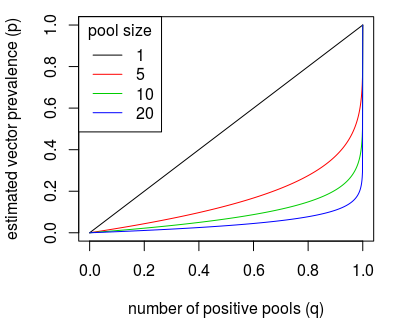
\includegraphics[height=6cm]{Figures/IndVsPool}
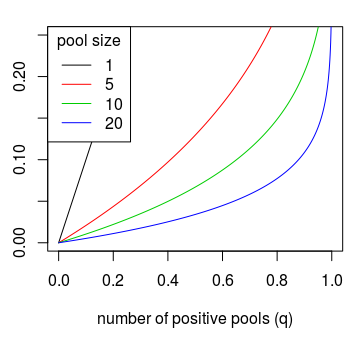
\includegraphics[height=6cm]{Figures/IndVsPoolZoom}
\end{array}$
\end{center}
\caption[Pool prevalence vs. actual prevalence.]{The relationship between vector prevalence ($p$) and pool prevalence ($q$) for different pool sizes if we assume large number of pools ($M$). Top: The relationship for all pool and vector prevalences. Bottom: Zoomed in on 0 - 20\% vector prevalence.}
\label{fig:pool}
\end{figure}

Figure \ref{fig:xeno} shows the reviewed data from Egypt \cite{Farid2007,Ramzy2006}, PNG \cite{Reimer2013_insecticidal,Weil2008} and Ghana \cite{Owusu2015} on a graph showing the relationship between vector prevalence and human mf prevalence for different proportions of parous mosquito (45\%, 60\% and 75\%). These studies all estimated vector prevalence from pooled prevalences, using similar methods to what we have described here, via commonly-used software tool PoolScreen. The lower part of the figure focuses on regions of low prevalence ($<10$\%), for which the model relationship is close to linear. Linear regression fits to the data show the differences between settings, indicating systematic differences in the mosquito dynamics. Even within one country, for example looking at Giza (yellow) and Qalubiya (red) there are potentially significant differences in the proportion of vectors that are parous. This reiterates the importance of having robust and well-characterised methods, involving understanding of the underlying dynamics, when interpreting vector measures of disease for public health applications.

\begin{figure}[ht]
\begin{center}$
\begin{array}{cc}
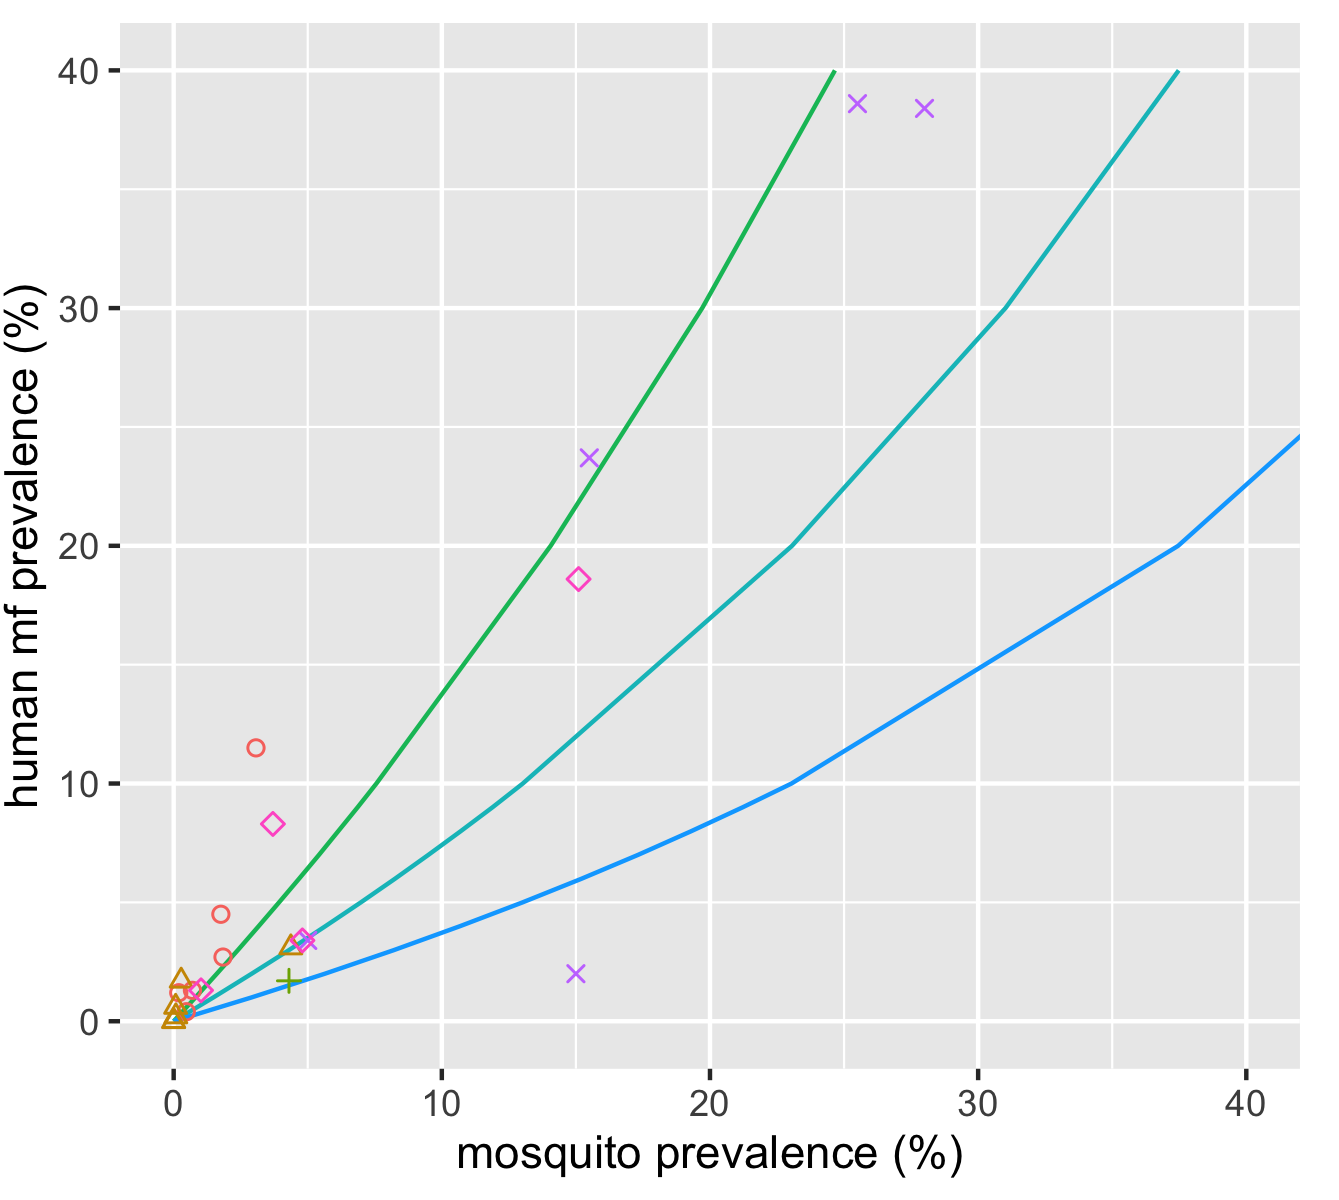
\includegraphics[height=6cm]{Project/Figures/Xeno/mfPrev_crop.png}
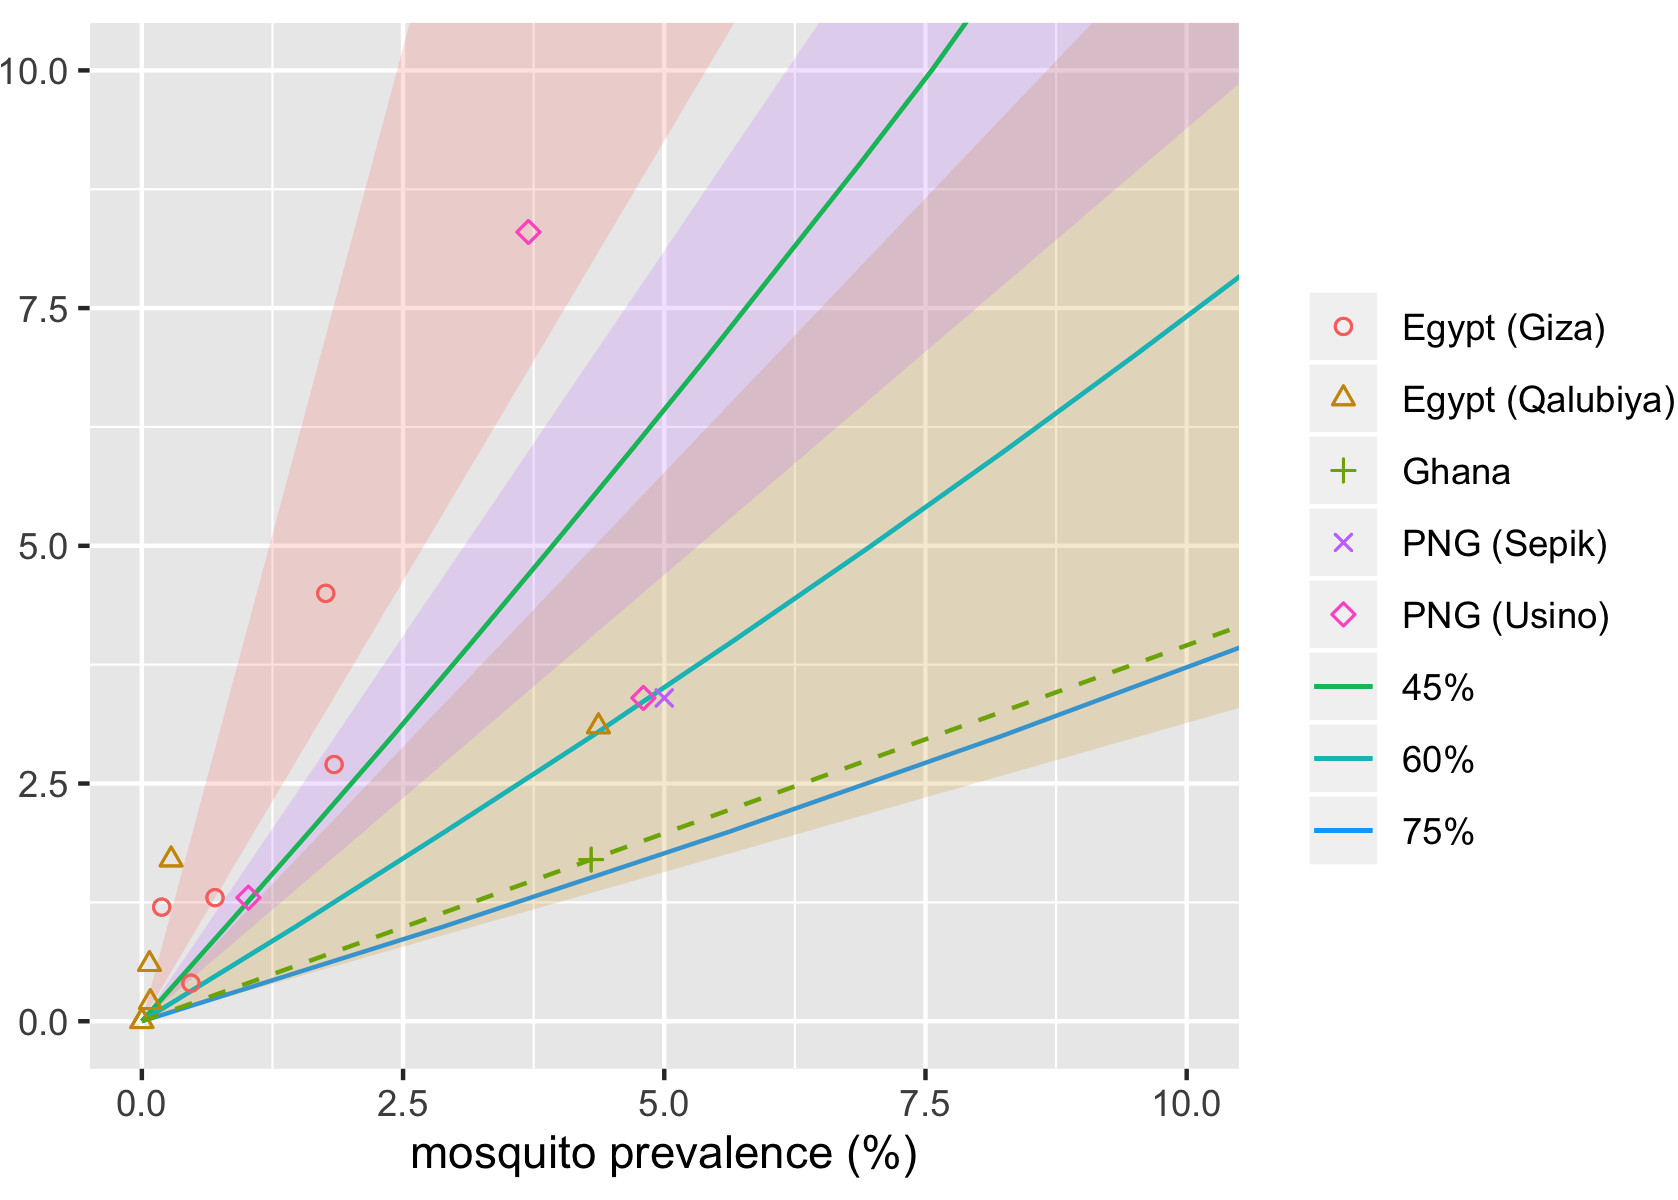
\includegraphics[height=6cm]{Project/Figures/Xeno/mfPrevZoomFit_crop.png}
\end{array}$
\end{center}
\caption[Xenomonitoring data with model comparison.]{Data and model linking vector prevalence and individual prevalence for different parity levels. In the data vector prevalence is estimated from pooled prevalence and the model shows curves for a range of parity (45\%, 60\% and 75\%). Right: Zoomed in to low prevalence ($<10$\%) with shaded regions representing uncertainty of fitted linear regressions to: a) Giza, Egypt \cite{Farid2007,Ramzy2006} (Red), b) Qalubiya, Egypt \cite{Farid2007,Ramzy2006} (yellow), c) Sepik \cite{Reimer2013_insecticidal} and Usino \cite{Weil2008}, PNG (purple). A dashed line shows the best fit for Ghana \cite{Owusu2015} but uncertainty cannot be calculated due to sample size.}
\label{fig:xeno}
\end{figure}

\begin{figure}[ht]
\begin{center}
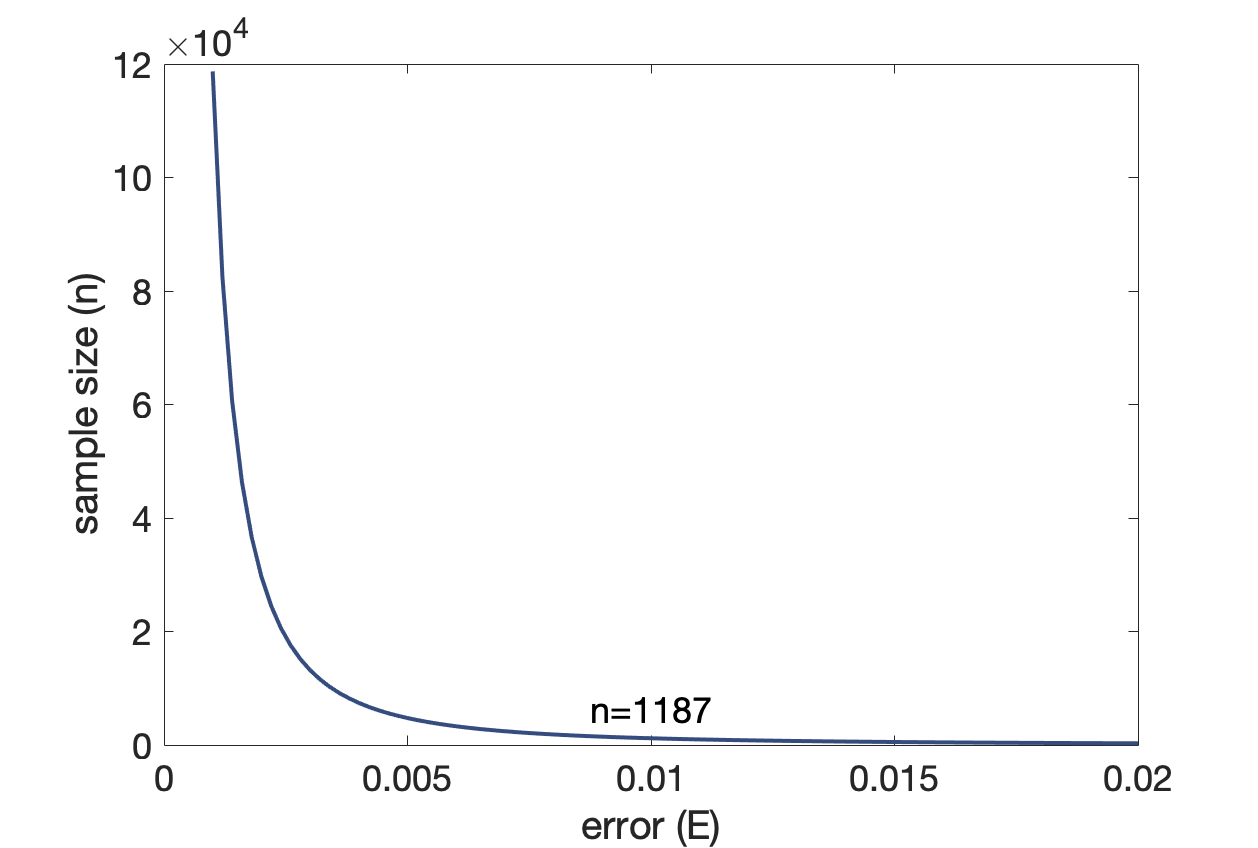
\includegraphics[height=7cm]{Project/Figures/Xeno/VaryError.png}
\end{center}
\caption[Sample size calculations.]{Plot showing how required sample size, $n$, of parous vectors varies with chosen error, $E$. Required sample size of random vectors, e.g. using light traps, is $m=an$. Here we take $a=10$ and the total number of vectors that need to be sampled is given by $n + m = n+an$.}
\label{fig:error}
\end{figure}

We are interested in the use of vector prevalence (either pooled or individual) ratios across trap types to estimate host prevalence, in particular whether required sample sizes are feasible for use of xenomonitoring as a surveillance method. Figure \ref{fig:error} shows how the required parous vector (gravid trap) sample size, $n$, varies with the size of the allowable error margin, $E$. A 1\% host mf prevalence error margin gives a required sample size of 1187 parous vectors, which translates to 11870 additional random vectors, giving an overall sample size of 13057 vectors. A smaller margin gives larger sample sizes; an error of 0.1\% prevalence giving sample sizes of $n=118,700$, $m=1,187,000$ and an overall sample size of 1,305,700.

\FloatBarrier

Using the relationships derived in this chapter we can run trial sampling scenarios, with fixed sample size and host prevalence, to compare the different methods of characterising uncertainty. A series of trial sampling scenarios were run with host prevalence $H=0.01$ or 1\% mf prevalence, a sample size of $n=1187$ and $m=11870$, as recommended by our sample size calculations, and a range of parity between 0.1 and 0.75. 

Figure \ref{fig:parity} shows parity estimates plotted against true underlying parity, with confidence intervals calculated using the Ln method (orange) and Delta method (blue). The main difference between the methods is that the Ln method is non-symmetrical around the central estimate, which in most cases leads to a narrower lower interval and a wider upper interval. However, aside from this small shift, there is generally good agreement between the two methods. The Delta method is the most widely used in statistics and is generalisable to more complex functions of random variables, so this method is the one that we use going forward.

\begin{figure}[ht]
\begin{center}
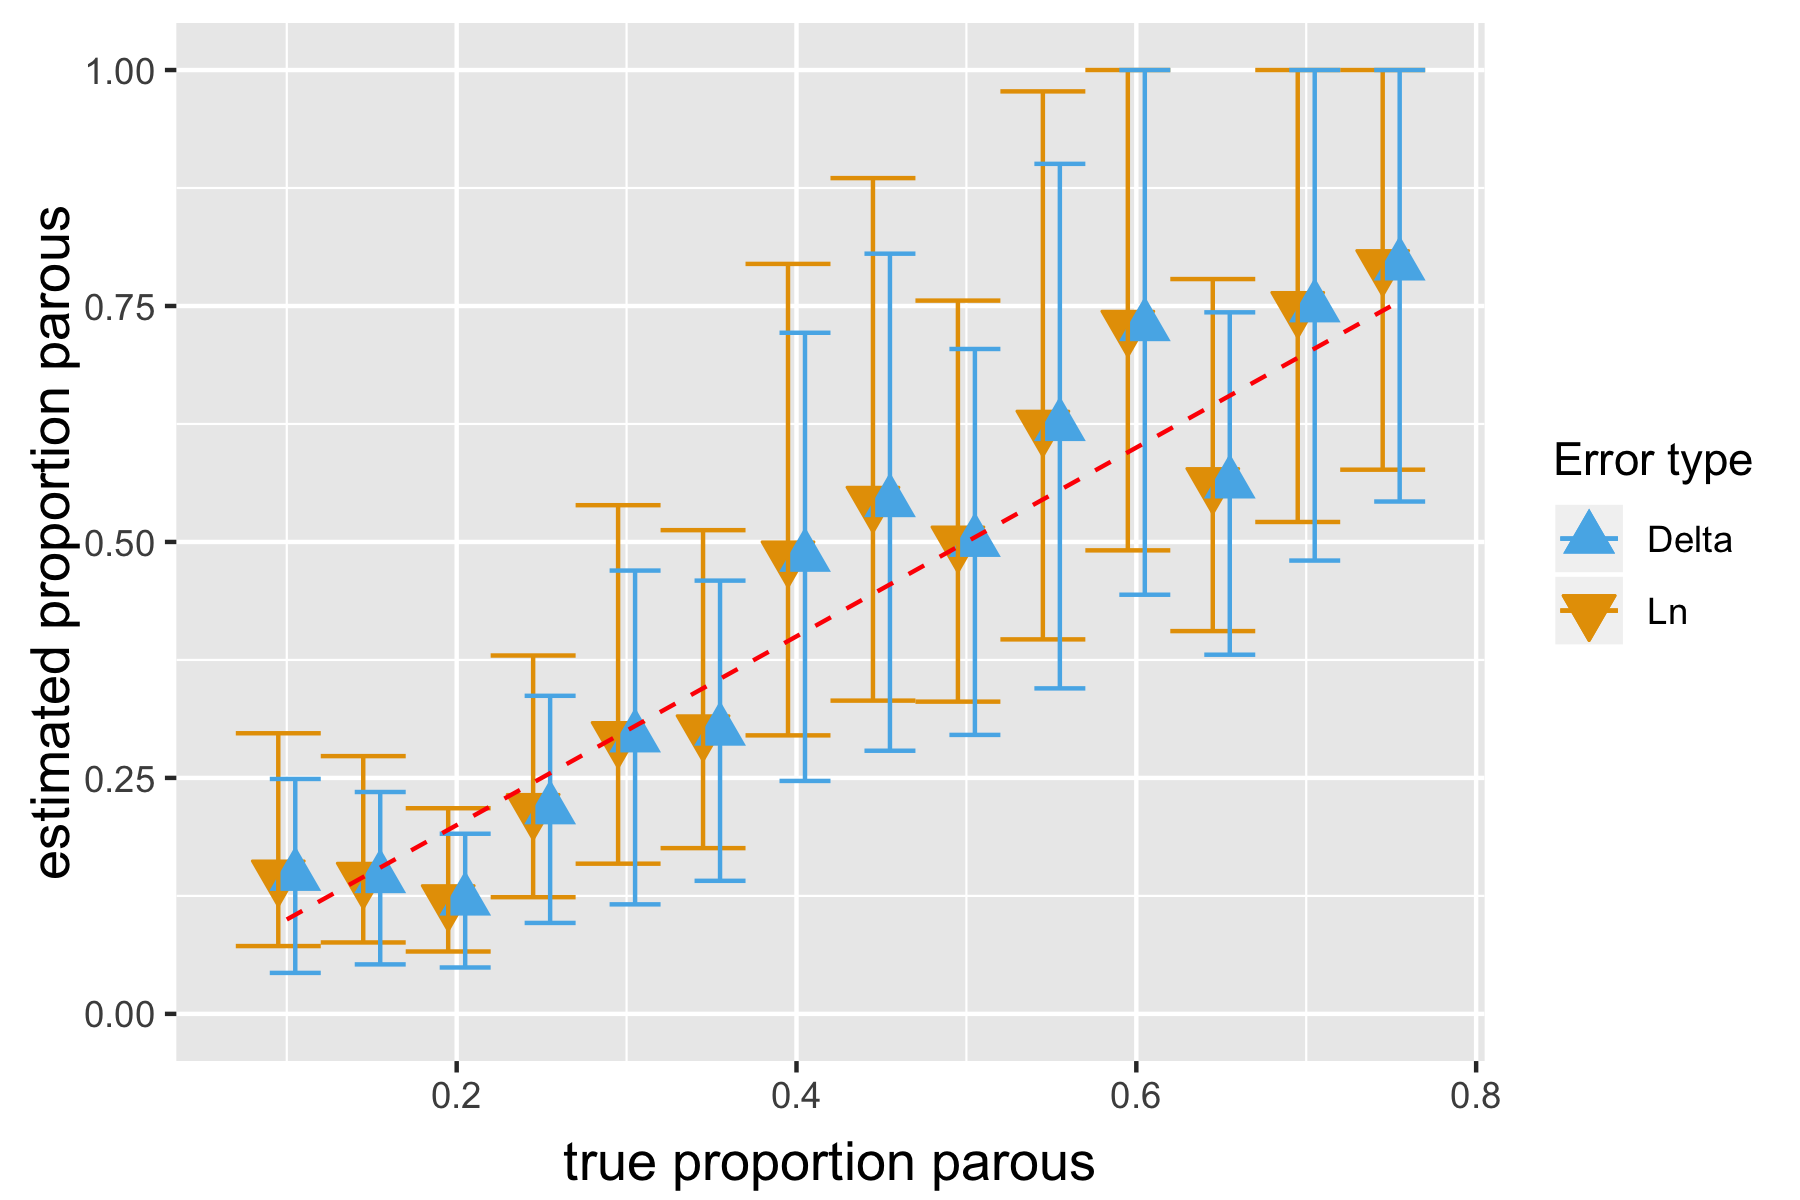
\includegraphics[height=8cm]{Project/Figures/Xeno/ParousEst.png}
\end{center}
\caption[Estimated vs. true proportion parous.]{Example simulation showing comparison between the two methods of confidence interval derivation for proportion of population parous when calculated from observed vector prevalence in gravid and random traps: Ln (orange, triangle) and Delta (blue, inverted triangle). Sample sizes: $n=1187$, $m=11870$ and underlying host prevalence $H=0.01$. Data points are offset to allow ease of viewing, neighboring points represent the same parous proportion.}
\label{fig:parity}
\end{figure}

Figure \ref{fig:vPrev} shows the estimated vector prevalence plotted against true vector prevalence for parous (orange) and random (blue) sampling of the population, with confidence intervals calculated using the Delta method. The randomly sampled vectors will include nulliparous mosquitoes which cannot test positive for LF presence as they haven't yet taken a bloodmeal, hence the random prevalence will always be less than the parous prevalence. As the sampling method takes into account trap efficiency, we have sampled ten times the number of random vectors as parous vectors, meaning the confidence intervals on these are narrower. However, the parous prevalence estimates are all within 0.5\% prevalence of the true value and the sampled data matches the true underlying value well.

\begin{figure}[ht]
\begin{center}
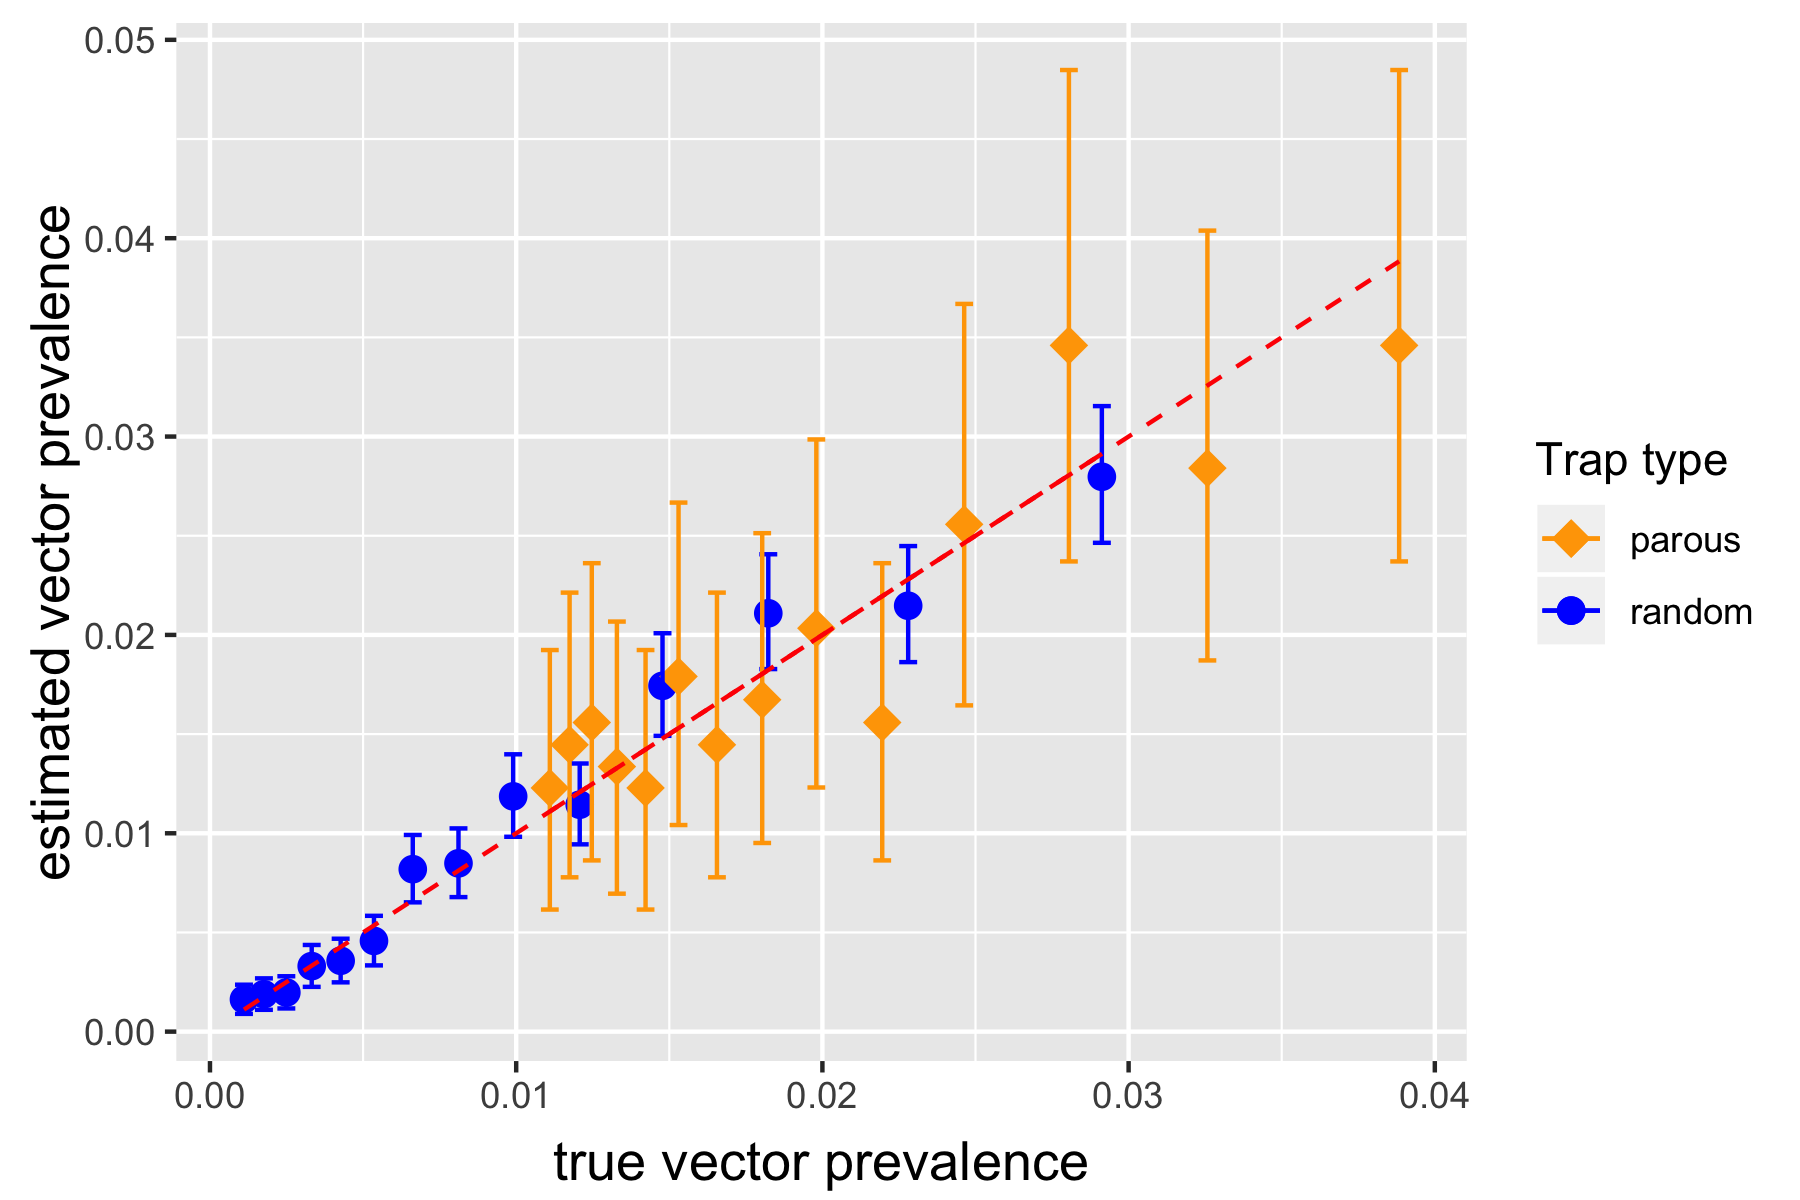
\includegraphics[height=8cm]{Project/Figures/Xeno/VPrevEst.png}
\end{center}
\caption[Estimated vector prevalence (parous and random).]{Example simulation showing the estimated vector prevalence in parous (orange, diamond) and random (blue, circle) populations, with sample sizes $n=1187$ and $m=11870$ respectively and underlying host prevalence $H=0.01$. Confidence intervals were calculated using the Delta method.}
\label{fig:vPrev}
\end{figure}

The next step is to consider the confidence intervals around the estimated host prevalence (see Figure \ref{fig:hPrev}). We compare the results of sampling individual vectors (red) and pooling the same number of total vectors into pools of $N=20$ (blue). This gives different estimates of host prevalence for the same underlying prevalence (1\%) and parity, and the Delta method was again used to calculate confidence intervals. In all cases, as expected due to loss of information through pooling, the pooled confidence intervals are either equivalent or wider than the individually sampled intervals. However, there is actually surprisingly little deviation in both the central estimates and confidence intervals between the two methods. This is potentially due to the simple near-linear relationship between pool prevalence and vector prevalence at low prevalence levels (Figure \ref{fig:pool}). Pooling vectors for testing is substantially cheaper and less labour intensive, so this could be exploited to increase feasibility of xenomonitoring as a survey tool.

The majority of the confidence intervals from individually tested vectors are less than 1\% prevalence on either side of the estimated host prevalence, whereas some of the confidence intervals from pooled testing are closer to 1.5\% each side. If pooling was being used then a larger sample size would be required for the same error width, but this would likely still represent fewer overall lab tests than using this sample size and individual testing.

\begin{figure}[ht]
\begin{center}
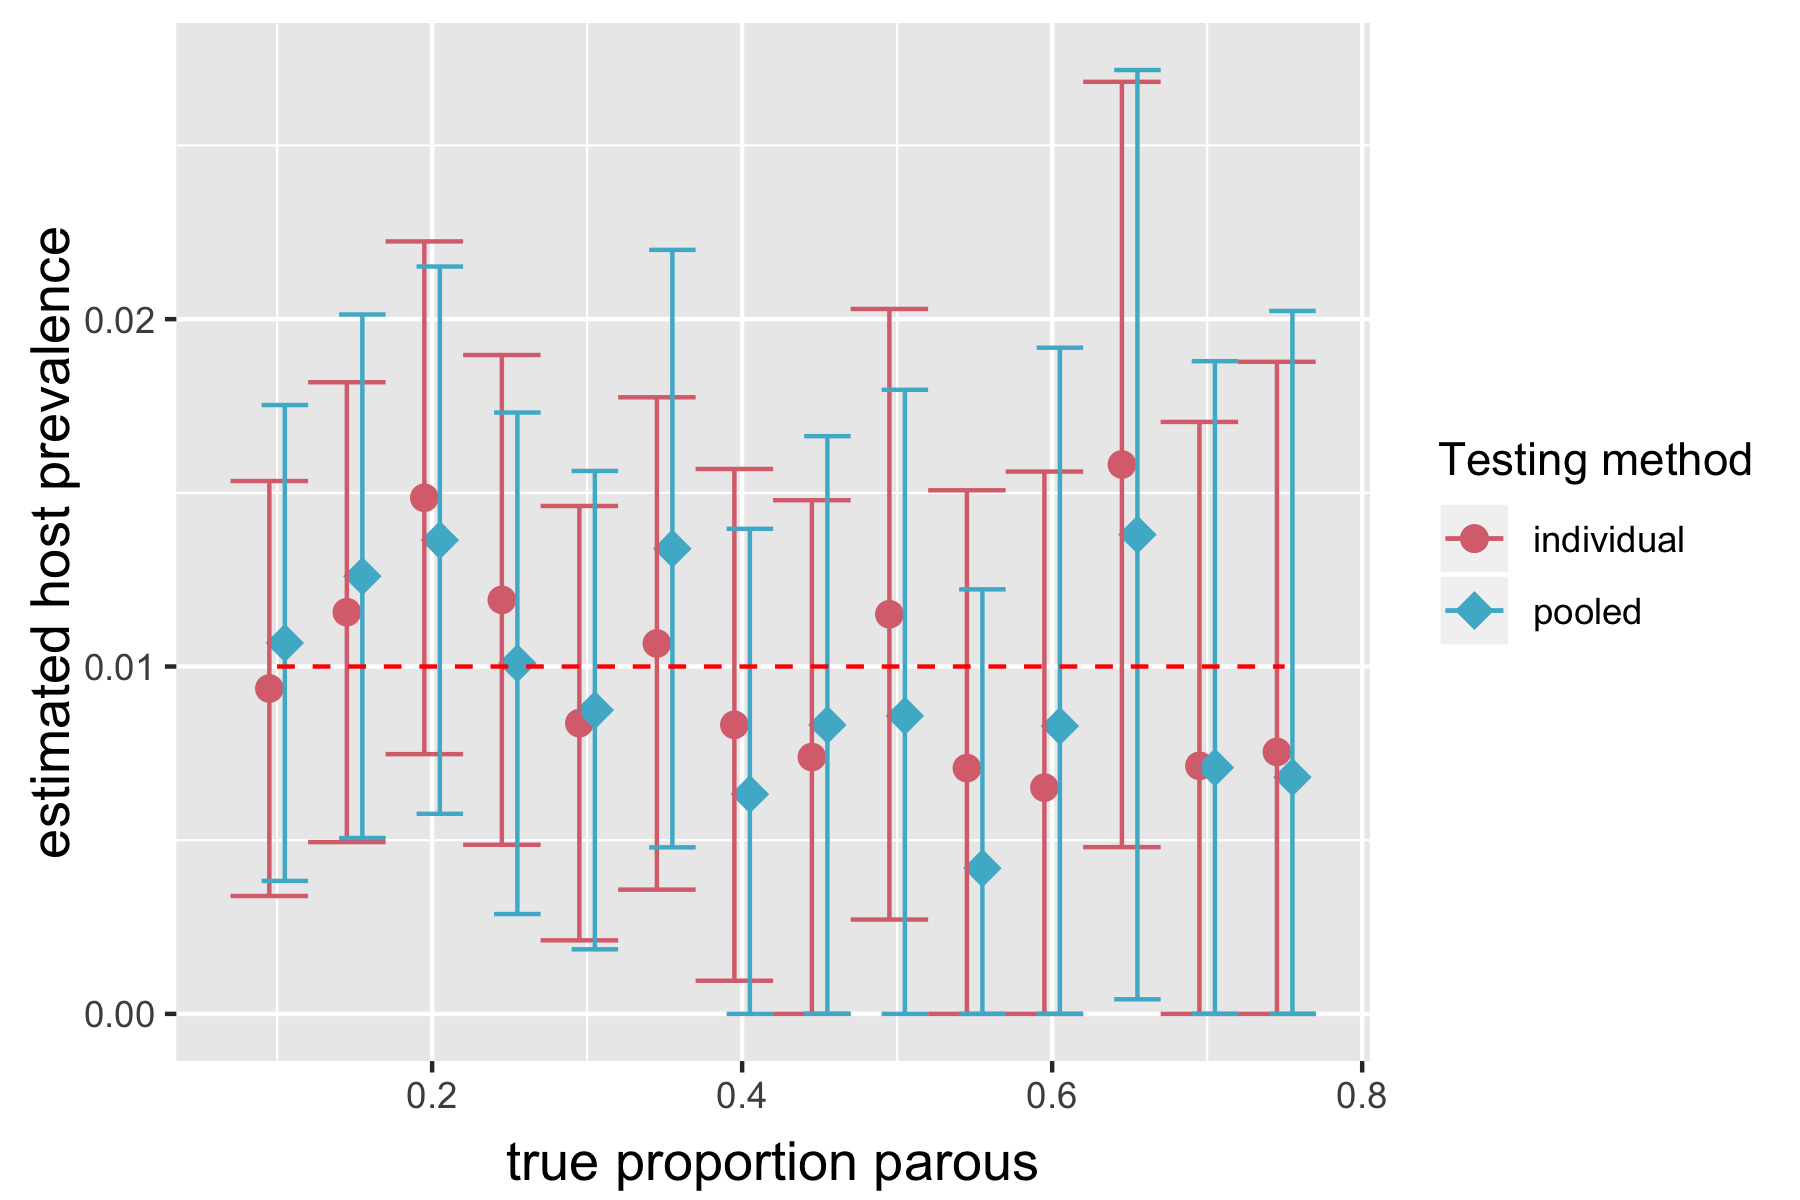
\includegraphics[height=9cm]{Project/Figures/Xeno/HPrevEst.png}
\end{center}
\caption[Estimated host prevalence (individual and pooled testing).]{Example simulation showing comparison of estimated host prevalence for individual (red, circle) and pooled (blue, diamond) tested mosquitoes. Sample sizes $n=1187$ and $m=11870$ respectively in both cases, with a pool size of $N=20$ in the pooled case, and underlying host prevalence $H=0.01$. Confidence intervals were calculated using the Delta method. Data points are offset to allow ease of viewing.}
\label{fig:hPrev}
\end{figure}

\FloatBarrier

\section{Discussion}

Through deriving analytical expressions for host prevalence as a function of vector DNA prevalence and subsequent confidence intervals, we have been able to calculate the vector sample sizes required to measure host prevalence to within a specified error with 95\% confidence. We have also demonstrated the potential of exploiting biases in different commonly used CDC-approved trap types as a proxy for measuring the proportions of nulliparous and parous mosquitoes, an essential locally-dependent parameter of vector and transmission dynamics. We also generalised these results to include the potential for pooling vectors before carrying out laboratory testing, which could substantially reduce costs and increase feasibility. These results are also directly applicable to other mosquito-borne diseases, such as malaria, as the biological details of LF are not used anywhere in this analysis.

We found that the relationship between pool prevalence and vector prevalence would be hard to use for mid to high vector prevalences ($>$20\% prevalence) due to the rapidly increasing slope. This would mean a small change in observed pool prevalence would lead to an increasingly large change in estimated vector prevalence, making it difficult to calculate vector prevalence to within a sensible error. However, at low vector prevalence ($<$20\%) this calculation becomes much more feasible, even for pool sizes of up to 20 vectors, and at very low prevalence ($<$5\%) the relationship between pool prevalence and vector prevalence is close to linear, allowing for very easy calculation.

Comparing the model of host prevalence as a function of prevalence to data observed in field studies demonstrated that parous proportions may vary significantly between settings, potentially due to local differences in the environment or vector dynamics.

When considering the required sample sizes used to measure vector and parous vector prevalence we estimated that a total sample size of just over 13,000 vectors (1187 parous, 11870 random) would be required to measure host prevalence to within an error of 1\% mf prevalence. This is a relatively large, but not infeasible, sample size. However, the required sample size increases exponentially with decreasing error, meaning the required precision of surveillance will be a key determining factor in whether xenomonitoring is a feasible method for post-MDA settings.

Cost of surveillance is also a key factor when programs consider which method to use. Both collection and PCR testing of mosquitoes are currently relatively high in cost due to the necessity of expensive real-time PCR machines \cite{Goodman2003} and skilled labour \cite{Okorie2016}, meaning individual capture and testing of vectors is likely to be infeasible in most settings. However, human surveillance is also a high cost intervention and is mainly used in post-MDA scenarios, where the low prevalences mean sample sizes need to be both large and spatially-distributed to effectively estimate presence or absence of transmission \cite{WHO2011}. The development of rapid point-of-care tests such as the filarial test strip (FTS) has alleviated some of these challenges, but many programs find there is a lack of willingness in the population to participate in surveillance for an infection is no longer considered a major problem \cite{Pilotte2016}.

Pooling vectors is common practice in the field, particularly if resources are limited, and can save substantially on PCR costs \cite{Okorie2016}. Our first investigations suggest that the difference in confidence between individually testing and pooling vectors is relatively small, potentially due to the low prevalence settings considered. We would expect this difference to be increased for higher prevalences, but as the main interest in xenomonitoring comes from elimination settings, pool sizes of up to 20 vectors in these places should only lead to a small loss of accuracy. More work needs to be done to directly link required sample size, pool size and error width. 

It is important to note that our assumption of zero co-variance between trap type samples only holds if traps are not set at the same time in the same place, as we might expect the presence of multiple trap types in one location to bias the samples. We have also assumed that the same number of vectors are included in each pool, which is not always the case in vector studies, often the average pool size is quoted instead. Further investigation would need to be done as to how feasible it is to fix pool size in the field and how variation in pool size might impact our calculations.

As more countries achieve EPHP and move into post-MDA surveillance, novel tools for monitoring infection levels become increasingly important. Human-based testing is expensive and invasive, with high associated labour and resource costs, and xenomonitoring has long been discussed as a potentially financially viable alternative but there is still little understanding of the relationship between vector prevalence and host prevalence and common opinion is that sample sizes may be logistically infeasible. We have attempted to bridge this knowledge gap and our findings suggest that sample sizes may be more feasible than expected, depending on required precision levels. However, we have presented analysis of one potential xenomonitoring surveillance method, further modelling and field work will be needed to investigate and compare a range of methods in developing the best tools for surveillance in the journey towards true elimination of transmission.

\subsection{Chapter Summary}

In this chapter I derived analytical relationships between host prevalence and measurable parasite DNA prevalence in vector blood meals, considering both individually sampled and pooled vector measurements. I also described a method for estimating the proportion of parous mosquitoes. I also derived an explicit formula for sample size calculation, depending on a required precision. My results show that required sample sizes may be more feasible than previously expected, and that pooling vectors may be a viable method for reducing the costs and labour required for use of xenomonitoring as a surveillance tool.

\FloatBarrier

\chapter{Aggregation}
\label{chap:AGG}

\section{Introduction}

\subsection{Chapter outline}

In this chapter, I explore the relationship between disease prevalence and infection intensity for helminth parasites. I challenge the standard negative binomial assumptions and briefly investigate the practical implications of such assumptions, particularly in conjunction with a range of mass drug administration (MDA) modelling assumptions. 

\section{Background}

As discussed in Chapter \ref{chap:STH}, disease prevalence ($P$) for helminth infections is often assumed to link to intensity (or mean worm burden, $M$) through a negative binomial distribution \cite{Anderson1992}. This is based on the knowledge that there is heterogeneity in the parasite burden between hosts, otherwise known as the aggregation of parasites within the host population. The derivation of this relationship is based on the assumption of a gamma-distributed infection risk combined with a Poisson distributed acquisition rate, giving the following analytical expression:

\begin{equation}
P = 1 - (1+M/k)^{-k}
\label{eqn:negbin1}
\end{equation}

Aggregation $k$ is expected to vary between settings, but is sometimes also taken as a function of $M$, linear or otherwise \cite{Norman2000_epifil, Anderson1992}. However, for modelling purposes aggregation is often considered constant for a particular region or setting.

This derivation has proved a highly powerful and useful tool in modelling helminth infections, however it is also considered by some as a non-ideal approximation, due to the increase in either biological or mathematical complexities often required to incorporate the negative binomial structure into models \cite{Yakob2014}. Converting results to prevalence also means that information is lost about the distribution of worm burden in the population, which is interlinked with the morbidity of disease and other important epidemiological factors. In particular, lower prevalence is associated with higher degrees of aggregation \cite{Truscott2019}.

However, unless the model is individual-based, prevalence measures are often used in the implementation of model simulations. For example, in vector-borne helminth infection models the force of infection from the host population to the vector population is often taken to be a function of the host prevalence rather than the mean worm burden, as it is necessary to include the probability of a vector biting an infectious individual. Ideally we would use a formulation based on $M$ rather than the host prevalence.

\section[LF]{Lymphatic filariasis force of infection}

If we consider the lymphatic filariasis (LF) model in Chapter \ref{chap:VEC}, then it is possible to describe such a formulation for the force of infection on the vector population as a function of $M$. To estimate host prevalence we consider the mf count per 20$\mu$l of blood in an individual as being distributed following a negative binomial distribution. From Anderson and May \cite{Anderson1992}, we have that the probability of $z$ parasites per 20$\mu$l of blood when sampling a random individual from the population is:
\begin{equation}
\mathbb{P}[z|M,k] = \binom{z+k-1}{z} \Big(1+\frac{M}{k}\Big)^{-k-z}\Big(\frac{M}{k}\Big)^z\,.
\label{eqn:negbin}
\end{equation}
Here $M$ is the mean mf count and $k$ is a descriptor of over-dispersion.

Take $A$ to be the ratio of mosquito feeding volume to 20$\mu$l, $A=($Feeding volume$)/20\mu$l, and $\eta$ to be the probability one ingested mf results in an L3 infection. Then, assuming a single hit model, it follows that the force of infection ($F_{H\rightarrow V}$) of humans on mosquitoes is proportional to the infinite sum:
\begin{equation}
F_{H\rightarrow V} \propto 1-\sum_{z=0}^{\infty}e^{-A\eta z}\mathbb{P}[z|M,k]\,.
\label{eqn:sum1}
\end{equation} 
We can now derive an analytical solution for the summation term, $\Sigma$, in Equation (\ref{eqn:sum1}). In order to use a binomial sums identity, 
\begin{equation}
\sum_{z=0}^{\infty}\binom{z+k-1}{z}x^{-z} \equiv \Big(\frac{x-1}{x}\Big)^{-k} \mbox{ for } |x|>1\,,
\end{equation}
we rearrange the summation term to fit this construction:
\begin{equation}
\Sigma =\bigg(1+\frac{M}{k}\bigg)^{-k}\sum_{z=0}^{\infty}\binom{z+k-1}{z}\bigg(e^{A\eta}\bigg(1+\frac{k}{M}\bigg)\bigg)^{-z}\,.
\end{equation}
Now, using the formula for $\mathbb{P}[z|M,K]$, as given in Equation (\ref{eqn:negbin}), and taking $x=e^{A\eta}(1+ k/M)$, we see that the force of infection is governed such that
\begin{equation}
F_{H\rightarrow V} \propto 1 - \bigg(1+\frac{M}{k}-\frac{M}{k}e^{-A\eta}\bigg)^{-k}\,.
\end{equation}

Unfortunately, there is a lack of data on the single hit probability of one mf translating into an L3 infection, $\eta$, leaving this formulation difficult to parameterise.

\section[MDA]{Impact of MDA on aggregation estimates}

In this section I compare population-based and individual-based formulations of infection to investigate the impact of different mass drug administration assumptions on aggregation assumption. 

For the population-based example I choose a constant aggregation parameter, $k$, to directly relate prevalence, $P$, to mean worm burden, $M$, using the standard negative binomial distribution. For the individual-based formulation I set up a population of size $N$ with individual worm burden distributed according to a negative binomial with a mean $M=1$ and aggregation $k=1$, such that each individual has an allocated worm burden drawn as random samples from this distribution.

For a given efficacy of treatment, $\alpha$, MDA is then applied to the individual-based population according to one of the following cases:
\begin{enumerate}
    \item Random human sampling for treatment and treatment efficacy per person sampled: either 100\% or 0\% clearance of infection based on an $\alpha$ probability of success.
    \item Random sampling, treatment efficacy per worm: an $\alpha$ probability of clearing each individual worm, independent of the number of worms present in a host.
\end{enumerate}

\begin{figure}[ht]
\begin{center}$
\begin{array}{cc}
\includegraphics[width=7.45cm]{Figures/Aggregation/prevVmwb.png}
\includegraphics[width=7.1cm]{Figures/Aggregation/prevVmda.png}\\
\includegraphics[width=7.45cm]{Figures/Aggregation/aggVmwb.png}
\includegraphics[width=7.1cm]{Figures/Aggregation/aggVmda.png}
\end{array}$
\caption[Aggregation and prevalence for different MDA assumptions.]{Relationships between mean worm burden, prevalence, parasite aggregation and MDA coverage for three cases: assuming MDA leads to proportional reduction of the mean with a constant aggregation parameter $k=1$ (black) and two cases of modelling one round of MDA coverage, with $k$ varied according to best fit negative binomial distribution. Case 1 (blue): MDA efficacy acts per person (either 0\% or 100\% of worms are cleared in each individual treated, with probability 0.88). Case 2 (red): MDA efficacy acts per worm (each worm in a treated human is cleared with probability 0.88). Host prevalence (top row) and parasite aggregation (bottom row) are given as functions of mean worm burden (left column) and MDA coverage (right column, efficacy $=88$\%).}
\label{fig:k}
\end{center}
\end{figure}

A negative binomial distribution is then fitted to the treated population and the new estimated value of the aggregation parameter, $k$, is recorded. Using this method we can numerically estimate $k$ for a range of mean worm burdens for both MDA assumption cases and then compare prevalence, using Equation \ref{eqn:negbin1}, to the population-level model using the constant value of $k$ (see Figure \ref{fig:k}). As the intervention modelled is one application of 88\% efficacy medication with a range of coverage between 0 and 100\%, the minimum possible resulting mean worm burden is 88\% less than baseline, which translates to a mean worm burden of 0.12.  

Our results show that assuming a constant $k$, and not re-fitting the negative binomial after applying an external force to the system, results in systematic over-estimation of prevalence compared to the individual-based model. Case 2 of modelling MDA (treatment efficacy per worm in each person treated) also results in a higher estimate of prevalence than Case 1 (treatment efficacy per person). This follows logically from the methods used, as assuming 100\% clearance in 88\% of cases treated will increase heterogeneity in worm burden and reduce prevalence.

We also see that the fitted aggregation parameter, $k$, varies dramatically with MDA coverage (and associated resulting mean worm burden). For Case 1 $k$ decreases with increasing MDA coverage and decreasing mean worm burden, and is close to zero at maximum coverage. This represents increasing heterogeneity as disease levels decline. Case 2 behaves similarly, albeit with a shallower gradient, until an MDA coverage of around 90\% (or a mean worm burden of around 0.2). At these high levels of coverage $k$ begins to increase again, representing reducing heterogeneity. As an effective coverage of higher than 90\% is infeasible in most settings \cite{Hussain2014,Babu2004}, with WHO recommended coverage of 65-80\% dependent on setting, this effect is interesting but has limited public health relevance.

\FloatBarrier

\subsection{Systematic non-adherence}

To consider the impact of extended MDA usage on aggregation we consider a sequence of four treatment rounds at a range of coverages (0-100\%), with the same initial conditions as before ($M=k=1$). Using Case 1 or Case 2 to model the MDA application, we can also consider the role of systematic non-adherence. We consider the two extreme cases: adherence is completely random, and adherence is completely systematic, i.e. the same individuals are treated in every round. 

\begin{figure}[h]
\begin{center}$
\begin{array}{cc}
\includegraphics[width=7.45cm]{Figures/Aggregation/prevVmwb_Sys.png}
\includegraphics[width=7.1cm]{Figures/Aggregation/prevVmda_Sys.png}\\
\includegraphics[width=7.45cm]{Figures/Aggregation/aggVmwb_Sys.png}
\includegraphics[width=7.1cm]{Figures/Aggregation/aggVmda_Sys.png}
\end{array}$
\caption[Aggregation and prevalence for systematic non-compliance.]{Relationships between mean worm burden, prevalence, parasite aggregation and MDA coverage for three cases: constant aggregation parameter $k=1$ (black), case 1 (blue) and case 2 (red) -- as described in Figure \ref{fig:k} --  after 4 rounds of MDA. Cases 1 and 2 are presented with random sampling (solid) and systematic non-compliance (dashed). Systematic non-compliance is taken to be maximal, with the same individuals missing treatment in each round. Host prevalence (top row) and parasite aggregation (bottom row) are given as functions of mean worm burden (left column) and MDA coverage (right column, efficacy $=88$\%).}
\label{fig:k_sys}
\end{center}
\end{figure}

Figure \ref{fig:k_sys} shows prevalence and $k$ for a range of MDA coverage and resulting mean worm burden. As expected, our results show that MDA programs with random adherence perform better than those with systematic adherence, due to a larger number of unique individuals treated. However, it's interesting to see that assuming random MDA coverage with treatment efficacy per worm leads to a substantially higher estimate of prevalence for the same mean worm burden than all other methods. The similarities between Case 1 and Case 2 in the case of complete systematic adherence implies that the reduction in aggregation caused by worm-based rather than human-based efficacy is overwhelmed by the increased aggregation caused by treating the same individuals each round. In all cases there are large discrepancies between the fitted estimates of prevalence and those calculated using a constant $k$. There is more noise in the non-systematic scenario of Case 2 than in other realisations because of the combined stochastic effects of randomly selecting both individual humans to treat and individual worms to clear in the presence of MDA, meaning a higher number of simulations would be required to achieve a comparably smooth curve.

\begin{figure}[h]
\begin{center}
\includegraphics[width=12.5cm]{Project/Figures/Aggregation/Case1Hist.png}\\
\includegraphics[width=12.5cm]{Project/Figures/Aggregation/Case2Hist.png}
\caption[Worm count frequency distributions.]{Example worm count frequency plots comparing systematic and random compliance for MDA cases 1 (Top, blue, drug efficacy per host) and 2 (Bottom, red, drug efficacy per worm). Worm counts are taken after 4 rounds of MDA at 65\% coverage in each case. MDA efficacy $=$ 88\%.}
\label{fig:kHist}
\end{center}
\end{figure}

Figure \ref{fig:kHist} depicts example worm count frequencies comparing systematic and random adherence across the two MDA modelling methods, assuming a coverage of 65\%. In both cases we see a decrease in the number of zeros and an overall increase in heterogeneity when we assume systematic adherence. Looking back at Figure \ref{fig:k_sys} we see that at 65\% MDA coverage there is a similar distance between systematic and random aggregation estimates for both cases, explaining the similarities between these two histograms.

\FloatBarrier

\section{Concluding remarks}

Using a simple individual-based formulation of parasite infection, I have shown that assuming a negative binomial relationship between mean worm burden and prevalence with constant aggregation, $k$, may not always be appropriate. In particular, MDA and the way it is modelled is likely to have effects on this relationship that cannot be characterised by a constant aggregation assumption. The relationships shown also demonstrate complex relationships between aggregation, MDA coverage, mean worm burden and prevalence. This implies that expressing $k$ as a linear function of mean worm burden may also be insufficient to capture changes in the underlying parasite distribution caused by external pressures.

We find that both systematic compliance and MDA assumptions have an impact on estimated distribution parameters and the associated aggregation, with systematic non-adherence resulting in potentially large changes in prevalence and aggregation estimates. These results highlight the importance of caution when translating between mean worm burden and prevalence across all helminth infections, as well as the need for further biological and modelling studies in the characterisation of these relationships.

\subsection{Chapter summary}

In this chapter I used an individual-based model to investigate the relationship between disease prevalence and infection intensity for helminth parasites, in particular focusing on analysis of the commonly-made negative binomial assumption. Considering a range of possible modelling assumptions, I demonstrated that assuming constant or linear values of the aggregation parameter, $k$, could potentially be inappropriate in a number of scenarios, resulting in an over-estimation of prevalence and an under-estimation of aggregation.


\chapter{Discussion}
\addcontentsline{toc}{chapter}{Discussion}


This thesis has focused on a range of questions across the landscape of neglected tropical diseases (NTDs), helminths and vector-borne transmission. The key overarching aim has been to investigate current models in the literature and expand the utility of these by including more detailed modelling of the underlying processes. A secondary, but equally important, goal was to highlight knowledge gaps and lay the basis for future research that will be beneficial towards disease control and elimination. I addressed these questions by developing novel models for \textit{A. lumbricoides} (a soil-transmitted helminth, STH) and lymphatic filariasis (LF) transmission using a variety of modelling methods. 

My results show that there are a number of scenarios where more detailed models would be appropriate to assist understanding of transmission and control. For example, I demonstrated in Chapter \ref{chap:STH} that the importance of seasonal mass drug administration (MDA) timing is highly dependent on local weather profiles, showing how temperate climates could be exploited to maximise program impact. In Chapters \ref{chap:ELIM} and \ref{chap:VEC} I showed that annual biting rate is a key determinant of elimination success and that vector control has the potential to substantially reduce transmission, in contradiction to previous modelling conclusions \cite{Irvine2017_Tripledrug}. In Chapter \ref{chap:XENO} I utilised an explicit model of mosquito feeding dynamics to calculate estimates of sample sizes required for the viable use of xenomonitoring as a tool for disease surveillance, which appear more feasible than suggested in the existing literature \cite{Schmaedick2014}.

The main implications of the seasonal model results in Chapter \ref{chap:STH} are that there may be a number of settings where MDA programs are a long way from achieving their potential maximum benefit. A relative improvement of 75\% across a four year period would represent a substantial gain in population health and disease control, particularly in settings that still see transmission after many rounds of MDA as benefits are expected to be multiplicative \cite{WHO2005_LF}. The recommendations prompted by these results are fairly simple and suggest that optimal treatment timing should coincide with environmental lows in the larval population \cite{Davis2018}. Similarly, the worst time for MDA was found to be during peaks in the infective larval population. As the relationship between temperature and development is reasonably well-characterised for ascaris eggs \cite{Wagner}, these periods should be relatively straightforward to determine.

The main bulk of the remaining chapters focused on aspects of the LF transmission cycle and their relationship with control and surveillance methods. Chapter \ref{chap:ELIM} has important connotations for future assessment and modelling of elimination dynamics. The identification of key knowledge gaps and recommendations for how they could be improved upon could potentially lead to substantially increased understanding of the disease \cite{Davis2019}, which could be instrumental in achieving elimination targets. Secondly, drawing awareness to the weaknesses in the experimental evidence base is vital to assuring models are realistic and well parameterised, highlighting the importance of critical assessment when taking parameters directly from the literature.

Findings from the mosquito model developed and analysed in Chapter \ref{chap:VEC}, show that adult-acting control measures are likely to have a much greater impact on transmission than larval-based interventions. Although larval control has been cited as a potentially viable method for reducing disease \cite{Kroeger1995}, these results demonstrate a multiplicative benefit of increasing coverage of adult-acting measures, compared to a linear benefit of increasing larvicide coverage. This implies that, unless vector population collapse is achieved through aggressive larvicide usage, programs would be better off focusing on long lasting insecticidal treated net (LLIN) and indoor residual spraying (IRS) interventions. The conclusion that high coverage (80\%) of LLIN usage alone could cause dramatic decreases in population mean worm burden across an order of 4-5 years. 

In addition, the recommendations for vector survey sample sizes and methods, presented in Chapter \ref{chap:XENO}, have far-reaching implications and potential impact. A statistically robust method of estimating the likely window of human prevalence from vector surveillance is critical to the feasibility of xenomonitoring as a public health tool and I have made substantial progress in this respect. The direct calculation of confidence intervals and guidelines on the sample sizes required for individually-sampled mosquitoes described here could lead to the development of a well-defined and applicable xeno-monitoring strategy that could be used by programs for surveillance post-validation of elimination as a public health problem.

My initial assessment that pooling vectors (up to and including pool sizes of 20) doesn't dramatically increase the error of measurements is a step towards making such strategies affordable and practically achievable for programs with fewer resources. I would expect that focusing on a low prevalence setting ($<$5\% microfilaria, mf, prevalence in humans) is the cause of this effect, making it ideal for elimination programs, but further analysis needs to be done to better understand this relationship.

I believe the consideration of aggregation assumptions in Chapter \ref{chap:AGG} is important, with results demonstrating that using a constant or linear form for the aggregation parameter, $k$, may be inappropriate for estimating prevalence from mean worm burden over time. However, this relatively short section of work serves only to demonstrate some potential pitfalls. Further work is necessary to characterise the extent of the limitations of the negative binomial assumption, as well as to develop a viable alternative if it is required.

My results are founded upon modelling assumptions. Parasite density dependent effects are neglected due to their reduced importance in low prevalence settings and other simplifications are assumed across the models, including constant pool sizes in the xenomonitoring analysis and no consideration of insecticide or chemotherapy resistance developing where control methods achieve high coverage.

Although it is important to take modelling assumptions into consideration when analysing results, I have demonstrated new methods for modelling helminth infections in humans and drawn some important conclusions. In some cases my results challenge the status quo, such as implying vector control usage may be more important than previously concluded in modelling studies. In other cases they confirm current understanding, for example by demonstrating why some regions may not see any seasonal variation in STH prevalence or intensity. In addition to these, I have also contributed some new understanding to the field, including a greater awareness of the importance of disease transmission parameters and novel suggestions for xenomonitoing error quantification.

The modelling undertaken during the work in this thesis is somewhat limited by the lack of general availability of detailed epidemiological data on the diseases discussed, both in terms of baseline and intervention measures. As such, the results are mainly theoretical and a key outcome is to highlight some areas where future modelling work, in collaboration with field observations, should be focused.

In particular, future modelling work is important around the dynamics of elimination of transmission of LF and how we can improve control methods for both LF and STH. Similar work investigating the impact of seasonal variation on transmission for other STH parasites would be important for deciding whether treatment programs should target their timing as the same drug is often used for multiple parasites, as well as extension of the present work to a wider range of settings and weather profiles. Greater clarity is also required on the characterisation of parasite aggregation within human populations under different external forces.

\chapter*{Concluding remarks}
\addcontentsline{toc}{chapter}{Concluding remarks}

The research reported in this thesis has investigated the impact of biological and environmental factors on neglected tropical disease (NTD) control, elimination and surveillance using mathematical and statistical modelling methods. I have demonstrated that challenging modelling assumptions and realising what we don't know can lead to deeper understanding of the processes involved, particularly where there is a paucity of data, and highlighted where further research is required. Through this work I have addressed some of the challenges faced by NTD control programs and my results contribute to the growing modelling evidence base within the field.

          %% this will do the appendices
%%TC:ignore
\bibliographystyle{unsrt}
\addcontentsline{toc}{chapter}{Bibliography}
\bibliographystyle{elsarticle-harv}
\bibliography{thesis}

%\bibliography{report}

\chapter*{Supplementary material}
\addcontentsline{toc}{chapter}{Supplementary material}
\begin{appendices}
\renewcommand\pagenumbering[1]{}

\chaptermark{Supplementary Material}
\section*{1. Further parameters for Chapter \ref{chap:VEC}}

This section of the supplementary contains detail on the standardisation of parameter names and meanings, as well as explicitly describing relationships between parameters where they exist. Table \ref{table:param} shows standard parameter names for vector models, aligned with Smith et al 2012 \cite{Smith2012}. Table \ref{table:param2} describes additional parameters defined for the purposes of the model used in Chapter \ref{chap:VEC}.

\begin{table*}[h]
\caption{Standard parameter names for vector models (Smith et al 2012).}% title of Table
\vspace{.1cm}
\centering % used for centering table
\begin{tabular}{l c c}% centered columns (4 columns)
\hline\hline                        %inserts double horizontal lines
Definition & Parameter & Notes \\ [0.5ex]% inserts table 
%heading
\hline                  % inserts single horizontal line
Population density of humans & $H$ &  \\
Population density of mosquitoes & $M$ &  \\
Number of infected humans & $X$ &  \\
Number of exposed vectors & $Y$ & $N_E$ \\
Number of infectious vectors & $Z$ & $N_I$ \\
Human blood feeding rate (daily) & $a$ & \\
Probability vector survives one day & $p$ & \\
Instantaneous vector death rate & $g$ & $g=-\ln(p)$  \\
Intrinsic incubation period (in humans) & $u$ & \\
Extrinsic incubation period (in vectors) & $v$ & \\
Human recovery rate & $r$ & \\
Prob vector infected after biting infected human & $c$ & \\
Prob infectious bite infects a human & $b$ & \\
Blood feeding rate (all prey) & $f$ & \\
Fraction of blood meals on humans & $Q$ & $a=fQ$ \\
Mean feeding cycle length & $\delta$ & $a=Q/\delta$\\
Prevalence of malaria in humans & $x$ & \\
Fraction of exposed vectors & $y$ & \\
Fraction of infectious vectors & $z$ & \\
Ratio of vectors to humans & $m$ & $=M/H$ \\
Human biting rate (\# bites per human per day) & $HBR$ & $=ma$\\
EIR (\# infectious bites per human per day) & $E$ & $=maz$ \\
The average mosquito lifespan & $1/g$ & \\
Stability index (\# human bites per vector across its life) & $S$ & $=a/g$\\
Probability vector survives to infectiousness & $P$ & $=e^{-gv}$\\
Probability vector infected during human bloodmeal & $\kappa$ & $=cx$\\
Vectorial capacity & $V$ & \\
Basic reproductive number & $R_0$ & \\
Effective reproductive number under control & $R_c$ & \\
Critical vector density required to sustain transmission & $m'$ & \\
      % [1ex] adds vertical space
\hline%inserts single line
\end{tabular}
\label{table:param}% is used to refer this table in the text
\end{table*}

\begin{table*}[h!]
\caption{Additional parameter names required for this model.}% title of Table
\vspace{.1cm}
\centering % used for centering table
\begin{tabular}{l c c}% centered columns (4 columns)
\hline\hline                        %inserts double horizontal lines
Definition & Parameter & Notes \\ [0.5ex]% inserts table 
%heading
\hline                  % inserts single horizontal line
Rate of moving from Exposed to Fed & $\pi_2$ & \\
Rate of moving from Fed to Resting & $\pi_3$ & \\
Rate of moving from Resting to Ovipositing & $\pi_4$ & \\
Rate of moving from Ovipositing to Exposed & $\pi_1$ & \\
Emergence rate (from larval stages) & $\beta$ & \\
Linear reduction in emergence rate due to larvicides & $\theta$ & \\
Additional IRS-induced death rate & $\gamma$ & \\
Bednet coverage & $\omega$ & \\
Probability successful feed in presence of bednet & $\sigma$ & \\
Probability death caused by bednet & $\nu$ & \\
Probability successful feed on single attempt & $q_1$ & $=1-Q\omega(1-\sigma)$ \\
Probability death on a single feeding attempt & $q_2$ & $=Q\omega\nu$\\
Probability a vector survives one feeding cycle & $K$ & previously $C$\\
The number of newly emerged null-parous vectors & $B_0$ &\\
Extrinsic incubation period (number of feeding cycles) & $N$ & \\
Probability of vector infection from one bite & $\hat{p}$ & $=xc$ \\
\hline%inserts single line
\end{tabular}
\label{table:param2}% is used to refer this table in the text
\end{table*}

\FloatBarrier

\section*{2. Published article 1}

\textbf{Title:} Seasonally timed treatment programs for Ascaris lumbricoides to increase impact -- An investigation using mathematical models.

\textbf{Authors:} \textbf{Emma L Davis}, Leon Danon, Joaquin M Prada, Sharmini A Gunawardena, James E Truscott, Johnny Vlaminck, Roy M Anderson, Bruno Levecke, Eric R Morgan, T Deirdre Hollingsworth.

\textbf{Journal:} PLOS Neglected Tropical Diseases.

\textbf{Date:} January 2019

\includepdf[pages=-,pagecommand={},width=\textwidth+2cm,offset=20 -20]{STHpaper.pdf}

\section*{3. Published article 2}

\textbf{Title:} Evaluating the evidence for lymphatic filariasis elimination.

\textbf{Authors:} \textbf{Emma L Davis}, Lisa J Reimer, Lorenzo Pellis, T Deirdre Hollingsworth.

\textbf{Journal:} Trends in Parasitology.

\textbf{Date:} November 2019

\includepdf[pages=-,pagecommand={},width=\textwidth+2cm,offset=20 -20]{LFpaper.pdf}

\section*{3. Published article 3}

\textbf{Title:} Complex interaction in soil-transmitted helminth co-infections from a cross sectional study in Sri Lanka.

\textbf{Authors:} Hannah C Lepper, Joaquin M Prada, \textbf{Emma L Davis}, Sharmini A Gunawardena, T Deirdre Hollingsworth.

\textbf{Journal:} Transactions of the Royal Society of Tropical Medicine and Hygiene.

\textbf{Date:} June 2018

\includepdf[pages=-,pagecommand={},width=\textwidth+2cm,offset=20 -20]{LepperPaper.pdf}
%%TC:endignore
%\chapter{Less obvious day of the week effects: additional figures}
%\input{../DOWChapter/DOW_appendix.tex}
\end{appendices}  

\end{document}
